% ******************************* PhD Thesis Template **************************
% Please have a look at the README.md file for info on how to use the template

%\documentclass[a4paper,12pt,times,numbered,print,index]{Classes/PhD/ThesisPSnPDF}
\documentclass[a4paper,12pt,times,numbered,print,index,custommargin]{Classes/PhDThesisPSnPDF}

%e-Energy 2018
\usepackage{mathtools}
\newcommand*\chem[1]{\ensuremath{\mathrm{#1}}}
\usepackage{tabularx}

% e-Energy 2019
\usepackage{tabularx}
\usepackage{multirow}
\usepackage{csvsimple}
\usepackage{mhchem}
\usepackage{graphicx}
\usepackage{subcaption}
\usepackage{mwe}
\usepackage{float}
\usepackage{placeins}
\usepackage{amsfonts}
\usepackage{booktabs}
\usepackage{siunitx}
\usepackage{array}
\usepackage{hyperref}
\usepackage{pdfpages}

% e-Energy 2020
\usepackage{tabularx}
\usepackage{multirow}
\usepackage{csvsimple}
\usepackage{mhchem}
\usepackage{graphicx}
\usepackage{subcaption}
\usepackage{mwe}
\usepackage{float}
\usepackage{placeins}
\usepackage{amsfonts}
\usepackage{booktabs}
\usepackage{siunitx}
\usepackage{array}
\usepackage{hyperref}
\usepackage{pdfpages}
\usepackage{algorithm}
\usepackage{algorithmicx}
\usepackage{algpseudocode}

%e-Energy 2020 AMLIES workshop
\usepackage{tabularx}
\usepackage{multirow}
\usepackage{csvsimple}
\usepackage{mhchem}
\usepackage{graphicx}
\usepackage{subcaption}
\usepackage{mwe}
\usepackage{float}
\usepackage{placeins}
\usepackage{amsfonts}
\usepackage{booktabs}
\usepackage{siunitx}
\usepackage{array}
\usepackage{hyperref}
\usepackage{pdfpages}
\usepackage{algorithm}
\usepackage{algorithmicx}
\usepackage{algpseudocode}




% ******************************************************************************
% ******************************* Class Options ********************************
% *********************** See README for more details **************************
% ******************************************************************************

% `a4paper'(The University of Cambridge PhD thesis guidelines recommends a page
% size a4 - default option) or `a5paper': A5 Paper size is also allowed as per
% the Cambridge University Engineering Deparment guidelines for PhD thesis
%
% `11pt' or `12pt'(default): Font Size 10pt is NOT recommended by the University
% guidelines
%
% `oneside' or `twoside'(default): Printing double side (twoside) or single
% side.
%
% `print': Use `print' for print version with appropriate margins and page
% layout. Leaving the options field blank will activate Online version.
%
% `index': For index at the end of the thesis
%
% `draftclassic': For draft mode without loading any images (same as draft in book)
%
% `draft': Special draft mode with line numbers, images, and water mark with
% timestamp and custom text. Position of the text can also be modified.
%
% `abstract': To generate only the title page and abstract page with
% dissertation title and name, to submit to the Student Registry
%
% `chapter`: This option enables only the specified chapter and it's references
%  Useful for review and corrections.
%
% ************************* Custom Page Margins ********************************
%
% `custommargin`: Use `custommargin' in options to activate custom page margins,
% which can be defined in the preamble.tex. Custom margin will override
% print/online margin setup.
%
% *********************** Choosing the Fonts in Class Options ******************
%
% `times' : Times font with math support. (The Cambridge University guidelines
% recommend using times)
%
% `fourier': Utopia Font with Fourier Math font (Font has to be installed)
%            It's a free font.
%
% `customfont': Use `customfont' option in the document class and load the
% package in the preamble.tex
%
% default or leave empty: `Latin Modern' font will be loaded.
%
% ********************** Choosing the Bibliography style ***********************
%
% `authoryear': For author-year citation eg., Krishna (2013)
%
% `numbered': (Default Option) For numbered and sorted citation e.g., [1,5,2]
%
% `custombib': Define your own bibliography style in the `preamble.tex' file.
%              `\RequirePackage[square, sort, numbers, authoryear]{natbib}'.
%              This can be also used to load biblatex instead of natbib
%              (See Preamble)
%
% **************************** Choosing the Page Style *************************
%
% `default (leave empty)': For Page Numbers in Header (Left Even, Right Odd) and
% Chapter Name in Header (Right Even) and Section Name (Left Odd). Blank Footer.
%
% `PageStyleI': Chapter Name next & Page Number on Even Side (Left Even).
% Section Name & Page Number in Header on Odd Side (Right Odd). Footer is empty.
%
% `PageStyleII': Chapter Name on Even Side (Left Even) in Header. Section Number
% and Section Name in Header on Odd Side (Right Odd). Page numbering in footer

% Uncomment to change page style
%\pagestyle{PageStyleII}

% ********************************** Preamble **********************************
% Preamble: Contains packages and user-defined commands and settings
% ******************************************************************************
% ****************************** Custom Margin *********************************

% Add `custommargin' in the document class options to use this section
% Set {innerside margin / outerside margin / topmargin / bottom margin}  and
% other page dimensions
%\ifsetCustomMargin
%  \RequirePackage[left=37mm,right=30mm,top=35mm,bottom=30mm]{geometry}
%  \setFancyHdr % To apply fancy header after geometry package is loaded
%\fi

\ifsetCustomMargin
\RequirePackage[left=30mm,right=20mm,top=20mm,bottom=20mm]{geometry}
\setFancyHdr % To apply fancy header after geometry package is loaded
\fi

% Add spaces between paragraphs
%\setlength{\parskip}{0.5em}
% Ragged bottom avoids extra whitespaces between paragraphs
\raggedbottom
% To remove the excess top spacing for enumeration, list and description
%\usepackage{enumitem}
%\setlist[enumerate,itemize,description]{topsep=0em}

% *****************************************************************************
% ******************* Fonts (like different typewriter fonts etc.)*************

% Add `customfont' in the document class option to use this section

\ifsetCustomFont
  % Set your custom font here and use `customfont' in options. Leave empty to
  % load computer modern font (default LaTeX font).
  %\RequirePackage{helvet}

  % For use with XeLaTeX
  %  \setmainfont[
  %    Path              = ./libertine/opentype/,
  %    Extension         = .otf,
  %    UprightFont = LinLibertine_R,
  %    BoldFont = LinLibertine_RZ, % Linux Libertine O Regular Semibold
  %    ItalicFont = LinLibertine_RI,
  %    BoldItalicFont = LinLibertine_RZI, % Linux Libertine O Regular Semibold Italic
  %  ]
  %  {libertine}
  %  % load font from system font
  %  \newfontfamily\libertinesystemfont{Linux Libertine O}
\fi

% *****************************************************************************
% **************************** Custom Packages ********************************

% ************************* Algorithms and Pseudocode **************************

%\usepackage{algpseudocode}


% ********************Captions and Hyperreferencing / URL **********************

% Captions: This makes captions of figures use a boldfaced small font.
%\RequirePackage[small,bf]{caption}

\RequirePackage[labelsep=space,tableposition=top]{caption}
\renewcommand{\figurename}{Fig.} %to support older versions of captions.sty


% *************************** Graphics and figures *****************************

%\usepackage{rotating}
%\usepackage{wrapfig}

% Uncomment the following two lines to force Latex to place the figure.
% Use [H] when including graphics. Note 'H' instead of 'h'
%\usepackage{float}
%\restylefloat{figure}

% Subcaption package is also available in the sty folder you can use that by
% uncommenting the following line
% This is for people stuck with older versions of texlive
%\usepackage{sty/caption/subcaption}
\usepackage{subcaption}

% ********************************** Tables ************************************
\usepackage{booktabs} % For professional looking tables
\usepackage{multirow}

%\usepackage{multicol}
%\usepackage{longtable}
%\usepackage{tabularx}


% *********************************** SI Units *********************************
\usepackage{siunitx} % use this package module for SI units


% ******************************* Line Spacing *********************************

% Choose linespacing as appropriate. Default is one-half line spacing as per the
% University guidelines

% \doublespacing
% \onehalfspacing
% \singlespacing


% ************************ Formatting / Footnote *******************************

% Don't break enumeration (etc.) across pages in an ugly manner (default 10000)
%\clubpenalty=500
%\widowpenalty=500

%\usepackage[perpage]{footmisc} %Range of footnote options


% *****************************************************************************
% *************************** Bibliography  and References ********************

%\usepackage{cleveref} %Referencing without need to explicitly state fig /table

% Add `custombib' in the document class option to use this section
\ifuseCustomBib
   \RequirePackage[square, sort, numbers, authoryear]{natbib} % CustomBib

% If you would like to use biblatex for your reference management, as opposed to the default `natbibpackage` pass the option `custombib` in the document class. Comment out the previous line to make sure you don't load the natbib package. Uncomment the following lines and specify the location of references.bib file

%\RequirePackage[backend=biber, style=numeric-comp, citestyle=numeric, sorting=nty, natbib=true]{biblatex}
%\bibliography{References/references} %Location of references.bib only for biblatex

\fi

% changes the default name `Bibliography` -> `References'
\renewcommand{\bibname}{References}


% ******************************************************************************
% ************************* User Defined Commands ******************************
% ******************************************************************************

% *********** To change the name of Table of Contents / LOF and LOT ************

%\renewcommand{\contentsname}{My Table of Contents}
%\renewcommand{\listfigurename}{My List of Figures}
%\renewcommand{\listtablename}{My List of Tables}


% ********************** TOC depth and numbering depth *************************

\setcounter{secnumdepth}{2}
\setcounter{tocdepth}{2}


% ******************************* Nomenclature *********************************

% To change the name of the Nomenclature section, uncomment the following line

%\renewcommand{\nomname}{Symbols}


% ********************************* Appendix ***********************************

% The default value of both \appendixtocname and \appendixpagename is `Appendices'. These names can all be changed via:

%\renewcommand{\appendixtocname}{List of appendices}
%\renewcommand{\appendixname}{Appndx}

% *********************** Configure Draft Mode **********************************

% Uncomment to disable figures in `draft'
%\setkeys{Gin}{draft=true}  % set draft to false to enable figures in `draft'

% These options are active only during the draft mode
% Default text is "Draft"
%\SetDraftText{DRAFT}

% Default Watermark location is top. Location (top/bottom)
%\SetDraftWMPosition{bottom}

% Draft Version - default is v1.0
%\SetDraftVersion{v1.1}

% Draft Text grayscale value (should be between 0-black and 1-white)
% Default value is 0.75
%\SetDraftGrayScale{0.8}


% ******************************** Todo Notes **********************************
%% Uncomment the following lines to have todonotes.

%\ifsetDraft
%	\usepackage[colorinlistoftodos]{todonotes}
%	\newcommand{\mynote}[1]{\todo[author=kks32,size=\small,inline,color=green!40]{#1}}
%\else
%	\newcommand{\mynote}[1]{}
%	\newcommand{\listoftodos}{}
%\fi

% Example todo: \mynote{Hey! I have a note}

% *****************************************************************************
% ******************* Better enumeration my MB*************
\usepackage{enumitem}


% ************************ Thesis Information & Meta-data **********************
% Thesis title and author information, refernce file for biblatex
% ************************ Thesis Information & Meta-data **********************
%% The title of the thesis
\title{Modelling the transition to a low-carbon energy supply}
%\title{Modelling the Transition to a Low-Carbon Energy Supply}
%\texorpdfstring is used for PDF metadata. Usage:
%\texorpdfstring{LaTeX_Version}{PDF Version (non-latex)} eg.,
%\texorpdfstring{$sigma$}{sigma}

%% Subtitle (Optional)
%\subtitle{Test}

%% The full name of the author
\author{Alexander John Michael Kell}

%% Department (eg. Department of Engineering, Maths, Physics)
\dept{School of Computing}

%% University and Crest
\university{Newcastle University}
% Crest minimum should be 30mm.
\crest{
\includegraphics[width=0.2\textwidth]{University_Crest.png}}
%% Use this crest, if you are using the college crest
%% Crest long miminum should be 65mm
%\crest{\includegraphics[width=0.45\textwidth]{University_Crest_Long}}

%% College shield [optional] 
% Crest minimum should be 30mm.
%\collegeshield{\includegraphics[width=0.2\textwidth]{CollegeShields/Kings}}


%% Supervisor (optional)
%% for multiple supervisors, append each supervisor with the \newline command
%\supervisor{Prof. A.B. Supervisor\newline
%Prof. C.D. Supervisor}

%% Supervisor Role (optional) - Supervisor (default) or advisor
% \supervisorrole{\textbf{Supervisors: }}
%% if no title is desired:
% \supervisorrole{}

%% Supervisor line width: required to align supervisors
%\supervisorlinewidth{0.35\textwidth}

%% Advisor (optional)
%% for multiple advisors, append each advisor with the \newline command
%\advisor{Dr. A. Advisor\newline
%Dr. B. Advisor}
     
%% Advisor Role (optional) - Advisor (default) or leave empty
% \advisorrole{Advisors: }
%% if no title is required
% \advisorrole{}

%% Advisor line width: required to align supervisors
%\advisorlinewidth{0.25\textwidth}


%% You can redefine the submission text:
% Default as per the University guidelines:
% ``This dissertation is submitted for the degree of''
%\renewcommand{\submissiontext}{change the default text here if needed}

%% Full title of the Degree
\degreetitle{Doctor of Philosophy}



%% Submission date
% Default is set as {\monthname[\the\month]\space\the\year}
%\degreedate{September 2014} 

%% Meta information
\subject{LaTeX} \keywords{{LaTeX} {PhD Thesis} {Engineering} {University of
Cambridge}}


% ***************************** Abstract Separate ******************************
% To printout only the titlepage and the abstract with the PhD title and the
% author name for submission to the Student Registry, use the `abstract' option in
% the document class.

\ifdefineAbstract
 \pagestyle{empty}
 \includeonly{Declaration/declaration, Abstract/abstract}
\fi

% ***************************** Chapter Mode ***********************************
% The chapter mode allows user to only print particular chapters with references
% Title, Contents, Frontmatter are disabled by default
% Useful option to review a particular chapter or to send it to supervisior.
% To use choose `chapter' option in the document class

\ifdefineChapter
 \includeonly{Chapter3/chapter3}
\fi

% ******************************** Front Matter ********************************
\begin{document}

\frontmatter

\maketitle

% ******************************* Thesis Dedidcation ********************************

\begin{dedication} 

I would like to dedicate this thesis to Sumiré and my loving parents\dots

\end{dedication}


% ******************************* Thesis Declaration ***************************

\begin{declaration}

I hereby declare that except where specific reference is made to the work of 
others, the contents of this dissertation are original and have not been 
submitted in whole or in part for consideration for any other degree or 
qualification in this, or any other university. This dissertation is my own 
work and contains nothing which is the outcome of work done in collaboration 
with others, except as specified in the text and Acknowledgements. This 
dissertation contains fewer than 65,000 words including appendices, 
bibliography, footnotes, tables and equations and has fewer than 150 figures.

% Author and date will be inserted automatically from thesis.tex \author \degreedate

\end{declaration}


% ************************** Thesis Acknowledgements **************************

\begin{acknowledgements}      


First, I would like to express my gratitude to my supervisors Dr Matthew Forshaw and Dr Stephen McGough. Who, without their support, guidance and insight I would have been unable to develop my skills in an academic context. Through their help and encouragements I have been able to exceed my own expectations.

Secondly, I would like to thank my parents and brother for supporting me during this time. Especially my father who has proved a guiding light during the most challenging parts. For example, inspiring my work on how disruption could be modelled with computational methods and pushing me to go further.

Thirdly I would like to thank Sumiré Moncholi for putting up with me during these years and providing daily support and care.

Since joining Newcastle University I have been helped and inspired by the vast range of problems and applications tackled within the School of Computing and the School of Mathematics, Statistics and Physics. In particular Junyang Wang, George Stamatiadis, Adam Cattermole, Kathryn Garside, Alexander Brown, Michael Dunne-Willows, Ashleigh McLean, Lauren Roberts, Thomas Cooper, Shane Halloran, Jonny Law, Peter Michalák, Saleh Mohamad and Mario Parreno.

I would also like to thank all my friends outside of the department during this time, especially Thomas Smith, Clement Venard, Sam Major, Marta Fernandez, Wenijan Yang, Alessandro Boussalem, Lars Eriksson, Tom Brunt, Owen Jones, Marianne Amor, Kevin Amor and Connor Scott.

Finally, I would like to thank my colleagues at the University of Cambridge's Centre for Science and Policy, for providing a challenging and stimulating environment to undertake an internship: Nicola Buckley, Katie Cohen, Rob Doubleday, Su Ford, Kate McNeil, Lauren Milden, Jackie Ouchikh, Erica Pramauro and Laura Sayer.

\end{acknowledgements}

\documentclass[11pt]{report}

\usepackage{a4wide}

\begin{document}
\begin{center}
	

\section*{Modelling the transition to a low-carbon energy supply}
\subsection*{Alexander J. M. Kell}
\end{center}

A transition to a low-carbon electricity supply is crucial to limit the impacts of climate change. Reducing carbon emissions could help prevent the world from reaching a tipping point, where runaway emissions are likely. Runaway emissions could lead to extremes in weather conditions around the world - especially in problematic regions unable to cope with these conditions. 


%A low-carbon transition in the electricity supply would enable sectors such as the automotive industry, indoor temperature regulation and manufacturing to decarbonise. 

However, the movement to a low-carbon energy supply can not happen instantaneously due to the existing fossil-fuel infrastructure and the requirement to maintain a reliable energy supply. Therefore, a low-carbon transition is required. Though, the decisions various stakeholders should make over the coming decades to reduce these carbon emissions are not obvious. This is due to many long-term uncertainties, such as electricity, fuel and generation costs, human behaviour and the size of electricity demand. In addition, the electricity generators invested in by generation companies are controlled by many heterogeneous actors in many markets around the world. These markets are known as decentralised electricity markets. Decentralised electricity markets stand in contrast to centralised control markets, where a central actor, such as a government, invest and control the market. A well choreographed low-carbon transition is, therefore, required between all of the heterogenous actors in the system, as opposed to changing the behaviour of a single, centralised actor.

To account for these long-term uncertainties in decentralised electricity markets, energy modelling can be used to aid stakeholders better understand the energy system. This allows for decisions to be made with more information. Energy models enable a quantitative analysis of how an electricity system may develop over the long term, and often use scenario analysis to investigate different decisions stakeholders could make. Simulations are powerful tools which can be used to generate insight, and are based upon the complexity of these models. Simulations are computer programs which have been designed to mimic a real-life system, to allow users to gain a better understanding of said system.


In this thesis, a novel agent-based simulation model, ElecSim, is created and used. ElecSim adopts an agent-based approach to simulation where each generation company within the system is modelled with its behaviour. This allows for fine-grained control and modelling of these generation companies. Thus allowing ElecSim to be used to investigate the following significant challenges in moving towards a low-carbon future:
\begin{enumerate}
	\item Predictions must be made to predict electricity demand at various time intervals in the future. We modelled the impact of poor predictions on generator investments and utilisation over the long-term.
	\item Devising a carbon tax can be challenging due to multiple competing objectives, and the inability for an iterative learning approach. In this work, we used ElecSim to model multiple different carbon tax policies using a genetic algorithm.
	\item Many decentralised electricity markets have become oligopolies, where a few generation companies own a majority of the electricity supply. In this thesis, we used reinforcement learning and ElecSim to find ways to ensure healthy competition.
\end{enumerate}

%What the problem is and how ElecSim helps.

This requires a number of core challenges to be addressed to ensure ElecSim is fit for purpose. These are:

\begin{enumerate}
%	\item The development of an open-source, long-term energy agent-based model of high temporal granularity.
	\item Development of the ElecSim model, where the replication of the pertinent features of the electricity market was required. For example, generation company investment behaviour, electricity market design and temporal granularity.
	\item The complexity of a model increases with the replication of increasing market features. Therefore, optimisation of the code was required to maintain computational tractability, to allow for multiple scenario runs. 
	\item Once the model has been developed, its long-term behaviour must be verified to ensure accuracy. In this work, cross-validation was used to validate ElecSim.
	\item To ensure that the salient parameters are found, a sensitivity analysis was run. In addition, various example scenarios were generated to show the behaviour of the model.
	\item Predicting short-term electricity demand is a core challenge for electricity markets. This is so that electricity supply can be matched with demand. In this work, various methodologies were used to predict demand 30 minutes and a day ahead. 
%	\item The validation of this model through the use of cross-validation.
%	\item Predicting electricity demand 30-minutes and a day-ahead, and observing the effects poor predictions have on the long-term electricity market.
%	\item Finding an optimal carbon tax to reduce both price and carbon emissions using this model.
%	\item Investigating the impact of collusion and market power in electricity markets.
\end{enumerate}



\end{document}


% *********************** Adding TOC and List of Figures ***********************

\tableofcontents

\listoffigures

\listoftables

% \printnomenclature[space] space can be set as 2em between symbol and description
%\printnomenclature[3em]
	
\printnomenclature

% ******************************** Main Matter *********************************
\mainmatter

%!TEX root = ../thesis.tex
%*******************************************************************************
%*********************************** First Chapter *****************************
%*******************************************************************************

\chapter{Getting started}  %Title of the First Chapter

\ifpdf
    \graphicspath{{Chapter1/Figs/Raster/}{Chapter1/Figs/PDF/}{Chapter1/Figs/}}
\else
    \graphicspath{{Chapter1/Figs/Vector/}{Chapter1/Figs/}}
\fi


%********************************** %First Section  **************************************
\section{What is loren ipsum? Title with math \texorpdfstring{$\sigma$}{[sigma]}} %Section - 1.1 

Hi Ipsum is simply dummy text of the printing and typesetting industry (see 
Section~\ref{section1.3}). Lorem Ipsum~\citep{Aup91} has been the industry's 
standard dummy text ever since the 1500s, when an unknown printer took a galley 
of type and scrambled it to make a type specimen book. It has survived not only 
five centuries, but also the leap into electronic typesetting, remaining 
essentially unchanged. It was popularised in the 1960s with the release of 
Letraset sheets containing Lorem Ipsum passages, and more recently with desktop 
publishing software like Aldus PageMaker including versions of Lorem 
Ipsum~\citep{AAB95,Con90,LM65}.

The most famous equation in the world: $E^2 = (m_0c^2)^2 + (pc)^2$, which is 
known as the \textbf{energy-mass-momentum} relation as an in-line equation.

A {\em \LaTeX{} class file}\index{\LaTeX{} class file@LaTeX class file} is a file, which holds style information for a particular \LaTeX{}.


\begin{align}
CIF: \hspace*{5mm}F_0^j(a) = \frac{1}{2\pi \iota} \oint_{\gamma} \frac{F_0^j(z)}{z - a} dz
\end{align}

\nomenclature[z-cif]{$CIF$}{Cauchy's Integral Formula}                                % first letter Z is for Acronyms 
\nomenclature[a-F]{$F$}{complex function}                                                   % first letter A is for Roman symbols
\nomenclature[g-p]{$\pi$}{ $\simeq 3.14\ldots$}                                             % first letter G is for Greek Symbols
\nomenclature[g-i]{$\iota$}{unit imaginary number $\sqrt{-1}$}                      % first letter G is for Greek Symbols
\nomenclature[g-g]{$\gamma$}{a simply closed curve on a complex plane}  % first letter G is for Greek Symbols
\nomenclature[x-i]{$\oint_\gamma$}{integration around a curve $\gamma$} % first letter X is for Other Symbols
\nomenclature[r-j]{$j$}{superscript index}                                                       % first letter R is for superscripts
\nomenclature[s-0]{$0$}{subscript index}                                                        % first letter S is for subscripts


%********************************** %Second Section  *************************************
\section{Why do we use loren ipsum?} %Section - 1.2


It is a long established fact that a reader will be distracted by the readable content of a page when looking at its layout. The point of using Lorem Ipsum is that it has a more-or-less normal distribution of letters, as opposed to using `Content here, content here', making it look like readable English. Many desktop publishing packages and web page editors now use Lorem Ipsum as their default model text, and a search for `lorem ipsum' will uncover many web sites still in their infancy. Various versions have evolved over the years, sometimes by accident, sometimes on purpose (injected humour and the like).

%********************************** % Third Section  *************************************
\section{Where does it come from?}  %Section - 1.3 
\label{section1.3}

Contrary to popular belief, Lorem Ipsum is not simply random text. It has roots in a piece of classical Latin literature from 45 BC, making it over 2000 years old. Richard McClintock, a Latin professor at Hampden-Sydney College in Virginia, looked up one of the more obscure Latin words, consectetur, from a Lorem Ipsum passage, and going through the cites of the word in classical literature, discovered the undoubtable source. Lorem Ipsum comes from sections 1.10.32 and 1.10.33 of "de Finibus Bonorum et Malorum" (The Extremes of Good and Evil) by Cicero, written in 45 BC. This book is a treatise on the theory of ethics, very popular during the Renaissance. The first line of Lorem Ipsum, "Lorem ipsum dolor sit amet..", comes from a line in section 1.10.32.

The standard chunk of Lorem Ipsum used since the 1500s is reproduced below for those interested. Sections 1.10.32 and 1.10.33 from ``de Finibus Bonorum et Malorum" by Cicero are also reproduced in their exact original form, accompanied by English versions from the 1914 translation by H. Rackham

``Lorem ipsum dolor sit amet, consectetur adipisicing elit, sed do eiusmod tempor incididunt ut labore et dolore magna aliqua. Ut enim ad minim veniam, quis nostrud exercitation ullamco laboris nisi ut aliquip ex ea commodo consequat. Duis aute irure dolor in reprehenderit in voluptate velit esse cillum dolore eu fugiat nulla pariatur. Excepteur sint occaecat cupidatat non proident, sunt in culpa qui officia deserunt mollit anim id est laborum."

Section 1.10.32 of ``de Finibus Bonorum et Malorum", written by Cicero in 45 BC: ``Sed ut perspiciatis unde omnis iste natus error sit voluptatem accusantium doloremque laudantium, totam rem aperiam, eaque ipsa quae ab illo inventore veritatis et quasi architecto beatae vitae dicta sunt explicabo. Nemo enim ipsam voluptatem quia voluptas sit aspernatur aut odit aut fugit, sed quia consequuntur magni dolores eos qui ratione voluptatem sequi nesciunt. Neque porro quisquam est, qui dolorem ipsum quia dolor sit amet, consectetur, adipisci velit, sed quia non numquam eius modi tempora incidunt ut labore et dolore magnam aliquam quaerat voluptatem. Ut enim ad minima veniam, quis nostrum exercitationem ullam corporis suscipit laboriosam, nisi ut aliquid ex ea commodi consequatur? Quis autem vel eum iure reprehenderit qui in ea voluptate velit esse quam nihil molestiae consequatur, vel illum qui dolorem eum fugiat quo voluptas nulla pariatur?"

1914 translation by H. Rackham: ``But I must explain to you how all this mistaken idea of denouncing pleasure and praising pain was born and I will give you a complete account of the system, and expound the actual teachings of the great explorer of the truth, the master-builder of human happiness. No one rejects, dislikes, or avoids pleasure itself, because it is pleasure, but because those who do not know how to pursue pleasure rationally encounter consequences that are extremely painful. Nor again is there anyone who loves or pursues or desires to obtain pain of itself, because it is pain, but because occasionally circumstances occur in which toil and pain can procure him some great pleasure. To take a trivial example, which of us ever undertakes laborious physical exercise, except to obtain some advantage from it? But who has any right to find fault with a man who chooses to enjoy a pleasure that has no annoying consequences, or one who avoids a pain that produces no resultant pleasure?"

Section 1.10.33 of ``de Finibus Bonorum et Malorum", written by Cicero in 45 BC: ``At vero eos et accusamus et iusto odio dignissimos ducimus qui blanditiis praesentium voluptatum deleniti atque corrupti quos dolores et quas molestias excepturi sint occaecati cupiditate non provident, similique sunt in culpa qui officia deserunt mollitia animi, id est laborum et dolorum fuga. Et harum quidem rerum facilis est et expedita distinctio. Nam libero tempore, cum soluta nobis est eligendi optio cumque nihil impedit quo minus id quod maxime placeat facere possimus, omnis voluptas assumenda est, omnis dolor repellendus. Temporibus autem quibusdam et aut officiis debitis aut rerum necessitatibus saepe eveniet ut et voluptates repudiandae sint et molestiae non recusandae. Itaque earum rerum hic tenetur a sapiente delectus, ut aut reiciendis voluptatibus maiores alias consequatur aut perferendis doloribus asperiores repellat."

1914 translation by H. Rackham: ``On the other hand, we denounce with righteous indignation and dislike men who are so beguiled and demoralized by the charms of pleasure of the moment, so blinded by desire, that they cannot foresee the pain and trouble that are bound to ensue; and equal blame belongs to those who fail in their duty through weakness of will, which is the same as saying through shrinking from toil and pain. These cases are perfectly simple and easy to distinguish. In a free hour, when our power of choice is untrammelled and when nothing prevents our being able to do what we like best, every pleasure is to be welcomed and every pain avoided. But in certain circumstances and owing to the claims of duty or the obligations of business it will frequently occur that pleasures have to be repudiated and annoyances accepted. The wise man therefore always holds in these matters to this principle of selection: he rejects pleasures to secure other greater pleasures, or else he endures pains to avoid worse pains."

\nomenclature[z-DEM]{DEM}{Discrete Element Method}
\nomenclature[z-FEM]{FEM}{Finite Element Method}
\nomenclature[z-PFEM]{PFEM}{Particle Finite Element Method}
\nomenclature[z-FVM]{FVM}{Finite Volume Method}
\nomenclature[z-BEM]{BEM}{Boundary Element Method}
\nomenclature[z-MPM]{MPM}{Material Point Method}
\nomenclature[z-LBM]{LBM}{Lattice Boltzmann Method}
\nomenclature[z-MRT]{MRT}{Multi-Relaxation 
Time}
\nomenclature[z-RVE]{RVE}{Representative Elemental Volume}
\nomenclature[z-GPU]{GPU}{Graphics Processing Unit}
\nomenclature[z-SH]{SH}{Savage Hutter}
\nomenclature[z-CFD]{CFD}{Computational Fluid Dynamics}
\nomenclature[z-LES]{LES}{Large Eddy Simulation}
\nomenclature[z-FLOP]{FLOP}{Floating Point Operations}
\nomenclature[z-ALU]{ALU}{Arithmetic Logic Unit}
\nomenclature[z-FPU]{FPU}{Floating Point Unit}
\nomenclature[z-SM]{SM}{Streaming Multiprocessors}
\nomenclature[z-PCI]{PCI}{Peripheral Component Interconnect}
\nomenclature[z-CK]{CK}{Carman - Kozeny}
\nomenclature[z-CD]{CD}{Contact Dynamics}
\nomenclature[z-DNS]{DNS}{Direct Numerical Simulation}
\nomenclature[z-EFG]{EFG}{Element-Free Galerkin}
\nomenclature[z-PIC]{PIC}{Particle-in-cell}
\nomenclature[z-USF]{USF}{Update Stress First}
\nomenclature[z-USL]{USL}{Update Stress Last}
\nomenclature[s-crit]{crit}{Critical state}
\nomenclature[z-DKT]{DKT}{Draft Kiss Tumble}
\nomenclature[z-PPC]{PPC}{Particles per cell}
%!TEX root = ../thesis.tex
%*******************************************************************************
%****************************** Second Chapter *********************************
%*******************************************************************************

\chapter{Background}
\label{chapter:background}
\ifpdf
    \graphicspath{{Chapter2/Figs/Raster/}{Chapter2/Figs/PDF/}{Chapter2/Figs/}}
\else
    \graphicspath{{Chapter2/Figs/Vector/}{Chapter2/Figs/}}
\fi


\section*{Prologue}

This chapter provides an overview of the relevant material which motivates and underpins the work carried out in this thesis. Section \ref{sec:intro:intro} introduces the problem domain and how such problems can be addressed. In Section \ref{sec:intro:elecmarketsmodelling} an introduction into how electricity markets are modelled. We provide an introduction in Section \ref{sec:intro:simulationmodelling} to simulation and machine learning. Finally, we conclude in Section \ref{sec:intro:conclusion}.


%\section{Introduction}
%\label{sec:intro:intro}
%
%The electricity market 

\section{Introduction to Electricity Markets}
\label{sec:intro:elecmarkets}

Electricity markets are complex. One of the principal reasons for this is the expense and difficulty of storing electricity. Additionally, as electricity travels over high voltage transmission lines, electricity doesn't always follow simple or unique paths, especially when the transmission lines become congested. Finally, electricity markets require technical overseers to ensure that the entire transmission system operates safely and reliably. 

Another aspect to consider is the fact that electricity is homogeneous. A single unit of electricity produced by a wind turbine is equivalent to a unit of electricity produced by a gas turbine. However, the functioning of different electricity producers, or generators, are not homogenous. Coal, gas and oil power plants can be \gls{dispatched} at the will of a human operator. Their ramp rates are well understood, as is the amount of fuel that is available. \Gls{ires}, however, such as solar, wind and tidal are dependent on the supply of solar irradiance, wind speed and the tide at any moment. Whilst these can be predicted, predictions are often wrong, and perfect knowledge is impossible. Therefore, at times where there is too much supply from \acrfull{ires} generators must be curtailed. In the opposite case, where there is too little supply from \acrshort{ires}, supply must be made up from other sources, such as coal, gas or hydro.

The environmental impact from different electricity generators differs significantly between generators. Whilst gas and coal can be dispatched at a time convenient to the grid operators, they emit \ce{CO2} along with other toxic substances. Wind and solar do not dispatch such substances or gases, but can not be controlled as easily. Storage technologies can be used to fill these gaps, however, large-scale storage depends on large pumped reservoirs that can move water to a higher position when demand for electricity is low, and supply is high. Not all geographies have access to such reservoirs, and therefore would rely on battery technology made from chemicals. However, reaching such high storage capabilities are expensive, and are yet to have been done in the real world. Another option is converting to electricity to hydrogen. However, this technology is also expensive and uncompetitive with traditional fossil fuels such as coal, gas and oil. Currently, \gls{peakerplants} are used to fill these gaps, however these plants are expensive to operate, highly polluting and use fossil fuels. It is expected that these \gls{peakerplants}s will be used increasingly due to the intermittent nature of renewable technologies. 


% Control of the grid (national grid) supply and demand
The electricity grid must match supply with demand at all times. Failure to do so results in an imbalance of supply and demand, and affects the frequency of the electricity network. Large differences between supply and demand can lead to blackouts or oversupply and damage equipment. A number of different markets exist to regulate the supply and demand, running from within seconds, to days-ahead and bilateral contracts which settle electricity for years ahead.

% Reserve, day-ahead, capacity market
There are a number of different market mechanisms that can be used to balance the supply and demand of electricity. Largely these can be divided between ancillary services and wholesale transactions. Wholesale transactions can occur as bilateral trades or on a day-ahead market. Bilateral trades can occur between two electricity suppliers and those that have an electricity demand. In this case, suppliers and customers create contracts for electricity in advance. Typically, these agents must let the market operator know of their trades. In a day-ahead market, the system price is, in principle, determined by matching offers from generators to bids from consumers at each node to develop a supply and demand equilibrium price. 

Ancillary markets, on the other hand, provide a method to facilitate and support the continuous flow of electricity so that supply continually meets demand. These include markets to regulate power and voltage control as well as frequency control. These markets make use of increasing supply or reducing demand at the times where this is required. 







\section{Introduction to Electricity Market Modelling}
\label{sec:intro:elecmarketsmodelling}
Test

\section{Introduction to Simulation and Machine Learning}
\label{sec:intro:simulationmodelling}
Test

\section{Conclusion}
\label{sec:intro:conclusion}
Test
%!TEX root = ../thesis.tex
%*******************************************************************************
%****************************** Third Chapter **********************************
%*******************************************************************************
\chapter{Literature review}
\label{chapter:litreview}
% **************************** Define Graphics Path **************************
\ifpdf
    \graphicspath{{Chapter3/Figs/Raster/}{Chapter3/Figs/PDF/}{Chapter3/Figs/}}
\else
    \graphicspath{{Chapter3/Figs/Vector/}{Chapter3/Figs/}}
\fi

\section*{Prologue}

In this chapter we give an introduction to the relevant energy modelling literature. We review the three major types of models: (1) optimisation models, (2) simulation models, and (3) equilibrium models. Section \ref{sec:litreview:energymodelling} gives an introduction to the field of energy modelling. In Section \ref{sec:litreview:optimisation} we introduce optimisation based models. Section \ref{sec:litreview:simulation} introduces simulation models and Section \ref{sec:litreview:equilibrium} introduces equilibrium models. We conclude this chapter in Section \ref{sec:litreview:conclusion}.

\section{Energy Modelling}
\label{sec:litreview:energymodelling}

In this thesis we define energy systems as the entire system from extraction of primary energy to use as final energy to supply services and goods \cite{Pfenninger2014a}. These systems can be modelled by different subsections which model technical, environmental and social elements. 

Energy models can typically be classified as top-down macro-economic models or bottom-up techno-economic models~\cite{Bohringer1998}. Top-down models typically focus on behavioural realism with a focus on macro-economic metrics. They are useful for studying economy-wide responses to policies ~\cite{Hall2016}, for example MARKAL-MACRO \cite{Fishbone1981} and LEAP \cite{Heaps2016}. Bottom-up models represent the energy sector in detail, and are written as mathematical programming problems~\cite{Gargiulo2013}. They detail technology explicitly, and can include cost and emissions implications~\cite{Hall2016}.

Within these two classifications, there exist four further paradigms of models within the community: (1) energy systems optimization models, (2) energy system simulation models, (3) power system and electricity market models and (4) qualitative and mixed methods scenarios \cite{Pfenninger2014a}. These four paradigms can be described as follows:

\begin{enumerate}
	\item These models cover the entire energy system and use optimization methods. The primary aim of these is to provide scenarios of how the system can involve.
	\item Models which cover the entire energy system using simulation techniques. These models have a primary purpose of providing forecasts of how the system may evolve.
	\item These models are focused exclusively on the electricity system. The methods and aims which underpin them vary between models. From optimization and scenarios to simulation and prediction.
	\item These models rely more on qualitative or mixed methods rather than quantitative approaches.
\end{enumerate}

In practice, it is possible for models to lie between any of these paradigms, and within a top-down or bottom-up approach. Table \ref{tab:intro:modeltypes} displays the model families, examples of such models and their primary focus.


\begin{table}[]
	\footnotesize
	\caption{Four different model types \cite{Pfenninger2014a}}
	\label{tab:intro:modeltypes}
	\begin{tabular}{@{}lll@{}}
		\toprule
		Model family                               & Examples                                 & Primary focus                            \\ \midrule
		Energy system optimisation models          & MARKAL~\cite{Fishbone1981a}, TIMES~\cite{Giannakidis2013}, MESSAGE~\cite{Schrattenholzer1981}, OSeMOSYS~\cite{Howells2011a}        & Normative scenarios                      \\
		Energy system simulation models            & LEAP\cite{LEAP2012a}, NEMS~\cite{Grozev2005a}, PRIMES\cite{Capros2012}                       & Forecasts, predictions                   \\
		Power system and electricity market models & WASP~\cite{WASP2001}, PLEXOS~\cite{PLEXOS2013}, EMCAS \cite{Conzelmann}, ElecSim\cite{Kell}             & Operational decisions \\
		Qualitative and mixed-methods scenarios    & DECC 2050 pathways, Stabilisation wedges & Narrative scenarios                      \\ \bottomrule
	\end{tabular}
\end{table}

Within these models, there is a dichotomy between planning models and operational models. Much work has been undertaken to understand the relationship between demand and supply, especially with the increase in \acrshort{ires}. Operational models allow for a high-resolution analysis of dispatch within an energy grid. Planning models allow for long-term analysis of systems, and have therefore, traditionally used a less fine spatial and temporal granularity. It is the case, however, that there is an amalgamation of these two approaches, as long-term planning on models also rely on high temporal and spatial granularity to accommodate \acrshort{ires}.

With \acrshort{ires} such as wind and solar power, output can vary temporally on many time scales. For example, there may be a gust of wind which lasts a number of seconds, or cloud cover which lasts for less than a minute. In an electricity grid, where supply must meet demand at all times, this can lead to challenges.

Currently, conventional technologies, provide a spinning reserve. Where a spinning reserve can increase or decrease capacity rapidly by increasing or decreasing the torque applied to a generator. However, if \acrshort{ires} is to reduce the size of this spinning reserve, then battery technologies will be required. It is for reasons such as this, that long-term energy models are requiring an increase in temporal granularity.





\section{Optimisation models}
\label{sec:litreview:optimisation}

Large bottom-up optimization models have long been used for energy system modelling. These are based upon a detailed description of the technical components of the energy system. However, because of their high detail, they must often make simplifications to remain tractable. Examples of these simplifications are to limit them to nationally aggregated technology build and yearly or seasonally averaged time-steps \cite{Pfenninger2014}. 

Optimisation models optimise a given quantity. These models generalise minimise costs or maximise welfare, defined as the material and physical well-being of people ~\cite{Keles2017}.  Examples of optimisation models are MARKAL/TIMES~\cite{Fishbone1981} and MESSAGE~\cite{Schrattenholzer1981}. MARKAL is possibly the most widely used general purpose energy systems model~\cite{Pfenninger2014}.

The majority of optimisation models use a linear programming (LP) approach, which for instance, minimise the total system cost, subject to a set of constraints. An example constraint could be that supply and demand are matched at all times in the grid. Mixed-integer liner programming (MILP) forces certain variables to be integers. This can enable the optimisation of the precise number of power plants or solar panels one should invest in \cite{Ringkjob2018}. It is possible to have non-linear optimisation models. These models use heuristic optimisation. Heuristic optimisation differs from traditional ptimisation modelling, in that they do not necessarily find the optimum solution \cite{Banos2011}.  

The MARKAL/TIMES model developed into TIAM (TIMES Integrated Assessment Model). TIAM is a global version of TIMES which also allows for climate response modelling. The MARKAL/TIMES family of models is developed by the IEA ETSAP. IEA ETSAP are a consortium of researchers from IEA member countries.

Both MARKAL/TIMES and MESSAGE represent possible scenarios of how the energy system may develop on a national, regional or global scale over a number of decades. However, these models do not state how likely each of these scenarios are to develop. These are both linear optimisation models which minimise the total energy system cost. Recent versions also allow for non-linear and mixed integer linear optimisations.

Hybrid models developed in the 1990s \cite{Economics2016}. Hybrid models link bottom-up models with top-down general equilibrium economic models. General equilibrium economic models attempt to characterize economy-wide movements in response to energy system changes. An example of such a model is the MESSAGE-MACRO model \cite{Messner2000} which soft-links two separate models. MESSAGE is a linear model which links to the non-linear MACRO model macroeconomic model. 

MESSAGE-MACRO soft-links these two models. This means that the two models are iteratively solved. In this case, the output from one is used as an input into the other. Over time this will hopefully lead to convergence. MARKAL-MACRO, however, \cite{mannewene92} hard-links the two models into one solution, which solves in a single iteration.

Even though these models have been the established approach for many decades, other examples of optimisation models are being developed. An open-source version of a similar style to MARKAL has been developed, known as OSeMOSYS \cite{Howells2011}. 

Traditional centralised optimisation models are not designed to  describe a system which is out of equilibrium. Optimisation models assume perfect foresight and risk neutral investments with no regulatory uncertainty. The core dynamics which emerge from equilibrium remain a black-box. For example, the model assumes a target will be reached, and does not provide information for which this is not the case. Reasons for this could be investment cycles which move the model away from equilibrium \cite{Chappin2017}.

\section{Simulation models}
\label{sec:litreview:simulation}

Simulation models simulate an energy system based upon specified equations, characteristics and rules. These are often bottom-up models, and are designed with a high level of technological description \cite{Ringkjob2018}. Agent-based models are a specific case of models, where actors are modelled explicitly as agents with heterogeneous strategies and behaviours.

Whilst energy optimisation models are built open mathematical formulations, simulation models can be built modularly and incorporate a range of methods. These simulation methods can also incorporate optimization based methods as submodules. Examples of these models are NEMS and PRIMES. NEMS is the U.S. Energy Information Administration's National energy Modelling System, whereas PRIMES covers the EU. These models have been used since the 1990s.

The Annual Energy Outlook is produced by NEMS and is used to inform policy decisions by the US Government. NEMS is made up of a number of submodules that are iteratively solved \cite{Gabriel2001}. Whilst each of the submodules can be implemented in different ways, the model can become complex, and therefore difficult to understand. 

PRIMES is also a modular system. An integrating module finds an equilibrium solution for energy supply, demand, cross-border energy trade, and emissions for all European countries \cite{Capros2012}. The analysis that PRIMES has provided has formed the basis of the EU's Energy Roadmap 2050 \cite{Gupta2011}.

LEAP (Long-range Energy Alternatives Planning System) is another simulation model and was developed by the Stockholm Environment Institute \cite{LEAP2012a}. LEAP provides an accounting system for supply with annual timesteps, but can also represent demand with a macroeconomic model. 


\subsection{Agent-based models}

However, electricity market liberalisation in many western democracies has changed the framework conditions. Centralised, monopolistic, decision making entities have given way to multiple heterogeneous agents acting for their own best interest~\cite{Most2010}. Policy options must therefore be used to encourage changes to attain a desired outcome. It is proposed that these complex agents are modelled using ABMs due to their non-deterministic nature. 

A number of ABM tools have emerged over the years to model electricity markets: SEPIA~\cite{Harp2000}, EMCAS~\cite{Conzelmann}, NEMSIM~\cite{Batten2006}, AMES~\cite{Sun2007}, GAPEX~\cite{Cincotti2013}, PowerACE~\cite{Rothengatter2007}, EMLab~\cite{Chappin2017} and MACSEM ~\cite{Praca2003}. Table \ref{table:tool_comparison} shows that these do not suit the needs of an open source, long-term market model. We will demonstrate that Monte-Carlo sampling of parameters is also required to increase realism.

There have been a number of recent studies using ABMs which focus on electricity markets, however they often utilize ad-hoc tools which are designed for a particular application \cite{Saxena2019, hadar2019, Kunzel2018}. ElecSim, however, has been built for re-use and reproducibility. The survey \cite{Weidlich2008} cites that many of these tools do not release source code or parameters, which is a problem that ElecSim seeks to address.

Table \ref{table:tool_comparison} contains six columns: tool name, whether the tool is open source or not, whether they model long-term investment in electricity infrastructure, and the markets they model. We determine how the stochasticity of real life is modelled, and determine whether the model is generalisable to different countries. 


An open source toolkit is important for reproducibility, transparency and lowering barriers to entry. It enables users to expand the model to their requirements and respective country. The modelling of long-term investment enables scenarios to emerge, and enable users to model investment behaviour. We demonstrate that the use of a Monte-Carlo method improves results.

SEPIA \cite{Harp2000} is a discrete event ABM which utilises Q-learning to model the bids made by GenCos. SEPIA models plants as being always on, and does not have an independent system operator (ISO), which in an electricity market, is an independent non-profit organization for coordinating and controlling of regular operations of the electric power system and market \cite{Zhou2007}. SEPIA does not model a spot market, instead focusing on bilateral contracts. As opposed to this, ElecSim has been designed with a merit-order, spot market in mind. As shown in Table \ref{table:tool_comparison}, SEPIA does not include a long-term investment mechanism. 

EMCAS ~\cite{Conzelmann} is a closed source ABM. EMCAS investigates the interactions between physical infrastructures and economic behaviour of agents. However, ElecSim focuses on the dynamics of the market, and provides a simplified, transparent model of market operation, whilst maintaining robustness of results.

NEMSIM \cite{Grozev2005} is an ABM that represents Australia's National Electricity Market (NEM). Participants are able to grow and change over time using learning algorithms. NEMSIM is non-generalisable to other electricity markets, unlike ElecSim.

AMES ~\cite{Sun2007} is an ABM specific to the US Wholesale Power Market Platform and therefore not generalizable for other countries. GAPEX \cite{Cincotti2013} is an ABM framework for modelling and simulating power exchanges . GAPEX utilises an enhanced version of the reinforcement technique Roth-Erev \cite{RothAE1995} to consider the presence of affine total cost functions. However, neither of these model the long-term dynamics for which ElecSim is designed.



PowerACE ~\cite{Rothengatter2007} is a closed source ABM of electricity markets that integrates short-term daily electricity trading and long-term investment decisions. PowerACE models the spot market, forward market and a carbon market. Similarly to ElecSim, PowerACE initialises GenCos with each of their power plants. However, as can be seen in Table \ref{table:tool_comparison}, unlike ElecSim, PowerACE does not take into account stochasticity of price risks in electricity markets ~\cite{Most2010}.

EMLab ~\cite{Chappin2017} is an open-source ABM toolkit for the electricity market. Like PowerACE, EMLab models an endogenous carbon market, however, they both differ from ElecSim by not taking into account stochasticity in the electricity markets, such as in outages, fuel prices and operating costs. After correspondence with the authors, however, we were unable to run the current version.

MACSEM \cite{Praca2003} has been used to probe the effects of market rules and conditions by testing different bidding strategies. MACSEM does not model long term investments or stochastic inputs.


As can be seen from Table \ref{table:tool_comparison}, none of the tools fill each of the characteristics we have defined. We therefore propose ElecSim to contribute an open source, long-term, stochastic investment model. 

\begin{table*}[]
	\centering
	\begin{adjustbox}{angle=90}
		\begin{tabular}{cccccc}
			%	\small	
			%	\begin{tabular}{c{2cm}c{0.8cm}c{1cm}c{0.8cm}c{1.2cm}c{1cm}}
			
			\multicolumn{1}{c}{\textbf{Tool name}} & \textbf{Open Source} & \textbf{Long-Term Investment} & \textbf{Market} & \textbf{Stochastic Inputs} & \textbf{Country Generalisability} \\ \midrule
			SEPIA \cite{Harp2000}  & \checkmark           & $\times$                             & \checkmark      & Demand                     & \checkmark                        \\ 
			EMCAS \cite{Conzelmann}   & $\times$                    & \checkmark                    & \checkmark      & Outages                    & \checkmark                        \\ 
			NEMSIM ~\cite{Batten2006}  & ?              & \checkmark                    & \checkmark      & $\times$                          & $\times$                                 \\ 
			AMES  ~\cite{Sun2007} & \checkmark           & $\times$                             & Day-ahead       & $\times$                          & $\times$                                 \\ 
			GAPEX  ~\cite{Cincotti2013} & ?              & $\times$                             & Day-ahead       & $\times$                          & \checkmark                        \\ 
			PowerACE \cite{Rothengatter2007} & $\times$                    & \checkmark                    & \checkmark      & Outages Demand             & \checkmark                        \\ 
			
			EMLab ~\cite{Chappin2017}  & \checkmark           & \checkmark                    & Futures         & $\times$                          & \checkmark                        \\ 
			MACSEM  ~\cite{Praca2003}  & ?              & $\times$                             & \checkmark      & $\times$                          & \checkmark                        \\ 
			ElecSim                                  & \checkmark           & \checkmark                    & Futures         & \checkmark                 & \checkmark                        \\ \hline
		\end{tabular}
	\end{adjustbox}
	\caption{Features of electricity market ABM tools.}
	\label{table:tool_comparison}
\end{table*}


\section{Equilibrium models}
\label{sec:litreview:equilibrium}

Equilibrium models take an economic approach. They model the energy sector as a part of the whole economy and study how it relates to the rest of the economy \cite{Ringkjob2018}. There exist two types of equilibrium models: general equilibrium models or computable general equilibrium models (CGE). These consider the whole economy, and determine the equilibrium across all markets, and determine important economic parameters such as the gross domestic product (GDP) endogenously. Partial equilibrium models (PE) focus on balancing one market. In this case, the market which is modelled is the electricity or energy market. They do not model the rest of the economy \cite{Ringkjob2018}. 

%\section{Models}
%\label{sec:litreview:models}
%
%Table goes here

\section{Conclusion}
\label{sec:litreview:conclusion}


Test
%!TEX root = ../thesis.tex
%*******************************************************************************
%****************************** Fourth Chapter **********************************
%*******************************************************************************
\chapter{ElecSim model}
\label{chapter:elecsim}

% **************************** Define Graphics Path **************************
\ifpdf
    \graphicspath{{Chapter3/Figs/Raster/}{Chapter3/Figs/PDF/}{Chapter3/Figs/}}
\else
    \graphicspath{{Chapter3/Figs/Vector/}{Chapter3/Figs/}}
\fi

\section*{Prologue}

In this Chapter we motivate and introduce the agent-based model, ElecSim. The majority of the work presented here was published in \cite{Kell} and \cite{Kell2020}. The contribution of this Chapter is a new open-source framework for the long-term modelling of electricity markets. We provide curated data, improve realism with Monte-Carlo sampling, and validate our model using genetic algorithm based optimisation. We validate our model between 2013 and 2018, as well as compare our model using the UK Government's baseline scenario. We provide a sensitivity analysis of important variables. 

We introduce our work in Section \ref{elecsim:sec:intro}, including why a simulation model is required to aid in a low carbon transition. We provide a literature review of work done to validate energy models in Section \ref{elecsim:sec:litreview}. The architecture of the model is presented in \ref{elecsim:sec:architecture}. The model is validated in Section \ref{elecsim:sec:validation}. Various scenarios are presented in Section \ref{elecsim:sec:scenarios}, where we vary demand until 2035. A sensitivity analysis is provided in \ref{elecsim:sec:sensitivity}, where we vary the weighted average cost of capital, as well as the down payment required for investments. Finally, we present the limitations of our model in Section \ref{elecsim:sec:limitations} and conclude our work in Section \ref{elecsim:sec:conclusions}.



%%%%%%%%%%%%%%%%%%%%%%%%%%%%%%%%%
%%%%%%%%%%%%%%%%% Paper 2
%%%%%%%%%%%%%%%%%%%%%%%%%%%%%%%%%
%
%
%
%
%	% Background
%	
%	Electricity market modelling is often used by governments, industry and agencies to explore the development of scenarios over differing timeframes. For example, what would the reduction in cost of renewable energy mean for investments in gas power plants or what would be an optimum strategy for carbon tax or subsidies? %Or, how might an increase in demand from electric vehicles impact on investment and electricity prices? 
%	
%	Optimization based solutions are the dominant approach for analysing energy policy. However, these types of models have certain limitations such as the need to be interpreted in a normative manner, and the assumption that the electricity market remains in equilibrium throughout. Through this work, we show that agent-based models are a viable technique to simulate decentralised electricity markets. The aim of this paper is to validate an agent-based modelling framework to increase confidence in its ability to be used in policy and decision making. 
%	
%	% Methodology
%	
%	
%	Our framework is able to model heterogeneous agents with imperfect information. The model uses a rules-based approach to approximate the underlying dynamics of a real life, decentralised electricity market. We use the UK as a case-study, however our framework is generalisable to other countries. We increase the temporal granularity of the model by selecting representative days of electricity demand and weather using a $k$-means clustering approach. 
%	
%	
%	% Results  
%	
%	
%	We show that our modified framework, ElecSim, is able to adequately model the transition from coal to gas observed in the UK between 2013 and 2018. We are also able to simulate a future scenario to 2035 which is similar to the UK Government, Department for Business and Industrial Strategy (BEIS) predictions, showing a more realistic increase in nuclear power over this time period. This is due to the fact that with current, large nuclear technology, electricity is generated almost instantaneously and has a low relative short-run marginal cost \cite{Department2016}. This low short-run marginal cost means that new nuclear will be dispatched on the electricity market once it has been turned on, and thus will not increase gradually.
%	
%	
%	
%	
%
%




\section{Introduction and Motivation}
\label{elecsim:sec:intro}

\subsection{Transition to a low-carbon energy supply}

Global carbon emissions from fossil fuels have significantly increased since 1900 \cite{boden2017global}.    Fossil-fuel based electricity generation sources such as coal and natural gas currently provide 65\% of global electricity. Low-carbon sources such as solar, wind, hydro and nuclear provide 35\% \cite{BP2018}. To halt this increase in \ce{CO2} emissions, a transition of the energy system towards a renewable energy system is required. 

% To achieve a low carbon energy infrastructure, and limit the effects of global warming, a transition in the electricity mix is required. Moving from a centralised and homogenous fossil fuel-based system to a distributed system based on renewable energy and batteries. % Batteries are required due to the fact that most renewable sources are effected by conditions outside the control of the owners (e.g. time of day, wind speed and cloud cover). This leads to a need for electricity to be stored at times when renewable production exceeds renewable energy supply, and for the batteries to be discharged at times of high electrical demand and low renewable energy supply. 




Such a transition needs to be performed in a safe and non-disruptive manner -- it may be possible to close down all fossil fuel plants in the next year, though if this leads to electricity shortages and power cuts then this is likely to cause significant problems both for industry and consumers. Therefore a stepped approach which allows seamless transfer is desirable. This may seem a simple process to achieve -- slowly phase out existing fossil fuel generators and replace these by renewable sources -- however, there are many risks and uncertainties in this process. Existing power plants have an expected lifetime and their owners wish to maximise this and the profits which can be made from them, renewable sources are still developing -- meaning that their efficiency and reliability will change in years to come.

Due to the long construction times, operating periods and high costs of power plants, investment decisions can have long term impacts on future electricity supply \cite{Chappin2017}. Governments and society, therefore, have a role in ensuring that the negative externalities of emissions are priced into electricity generation. This is most likely to be achieved via a carbon tax and regulation to influence electricity market players such as \acrfull{gencos}.


Decisions made in an electricity markets may have unintended consequences due to their complexity. A method to test hypothesise before they are implemented would therefore be useful.

To aid in such a transition, energy modelling can be used by governments, industry and agencies to explore possible scenarios under different variants of government policy, future electricity generation costs and energy demand. These energy modelling tools aim to mimic the behaviour of energy systems through different sets of equations and data sets to determine the energy interactions between different actors and the economy \cite{Machado2019}.





\subsection{ElecSim: Modelling and simulation}




Live experimentation of physical processes is not often practical. The costs of real life experimentation can be prohibitively high, and can require a significant amount of time in order to fully ascertain the long-term trends. There is also a risk that changes can have detrimental impacts and lead to risk-averse behaviour. These factors are true for electricity markets, where decisions can have long term impacts. Simulation, however, can be used for rapidly prototyping ideas. The simulation is parametrised by real world data and phenomena. Through simulation, the user is able to assess the likelihoods of outcomes under certain scenarios and parameters \cite{Law:603360}.





Simulation is often used to increase understanding as well as to reduce risk and reduce uncertainty. Simulation allows practitioners to realise a physical system in a virtual model. In this context, a model is defined as an approximation of a system through the use of mathematical formulas and algorithms. Through simulation, it is possible to test a system where real life experimentation would not be practical due to reasons such as prohibitively high costs, time constraints or risk of detrimental impacts. This has the dual benefit of minimising the risk of real decisions in the physical system, as well as allowing practitioners to test less risk-averse strategies.

\acrfull{abms} are a class of computational simulation models composed of autonomous, interacting agents and model the dynamics of a system. Due to the numerous and diverse actors involved in electricity markets, \acrshort{abms} have been utilised in this field to address phenomena such as market power \cite{Ringler2016a}. 

The work presented in this Chapter develops ElecSim, an open-source \acrshort{abm} that simulates GenCos in a wholesale electricity market. ElecSim models each GenCo as an independent agent and electricity demand. An electricity market facilitates trades between the two. 

GenCos make bids for each of their power plants. Their bids are based on the generators \gls{SRMC} \cite{Perloff2012}, which excludes capital and fixed costs. The electricity market accepts bids in cost order, also known as merit-order dispatch. GenCos invest in power plants based on expected profitability.	

ElecSim is designed to provide quantitative advice to policy makers, allowing them to test policy outcomes under different scenarios. They are able to modify a scenario file to realise a scenario of their choice. It can also be used by energy market developers who can test new electricity sources or policy types, enabling the modelling of changing market conditions.

 This model can be used by the following players:
 
 \begin{itemize}
 \item {\bf Policy experts} to test policy outcomes under different scenarios and provide quantitative advice to policy makers. They can provide a simple script defining the policies they wish to use along with the parameters for these polices.
 \item {\bf Energy market developers} who can use the extensible framework to add such things as new energy sources, policy types, consumer profiles and storage types. Thus allowing ElecSim to adapt to a changing ecosystem.
 \end{itemize}
 



% \begin{figure}
% \centering
% 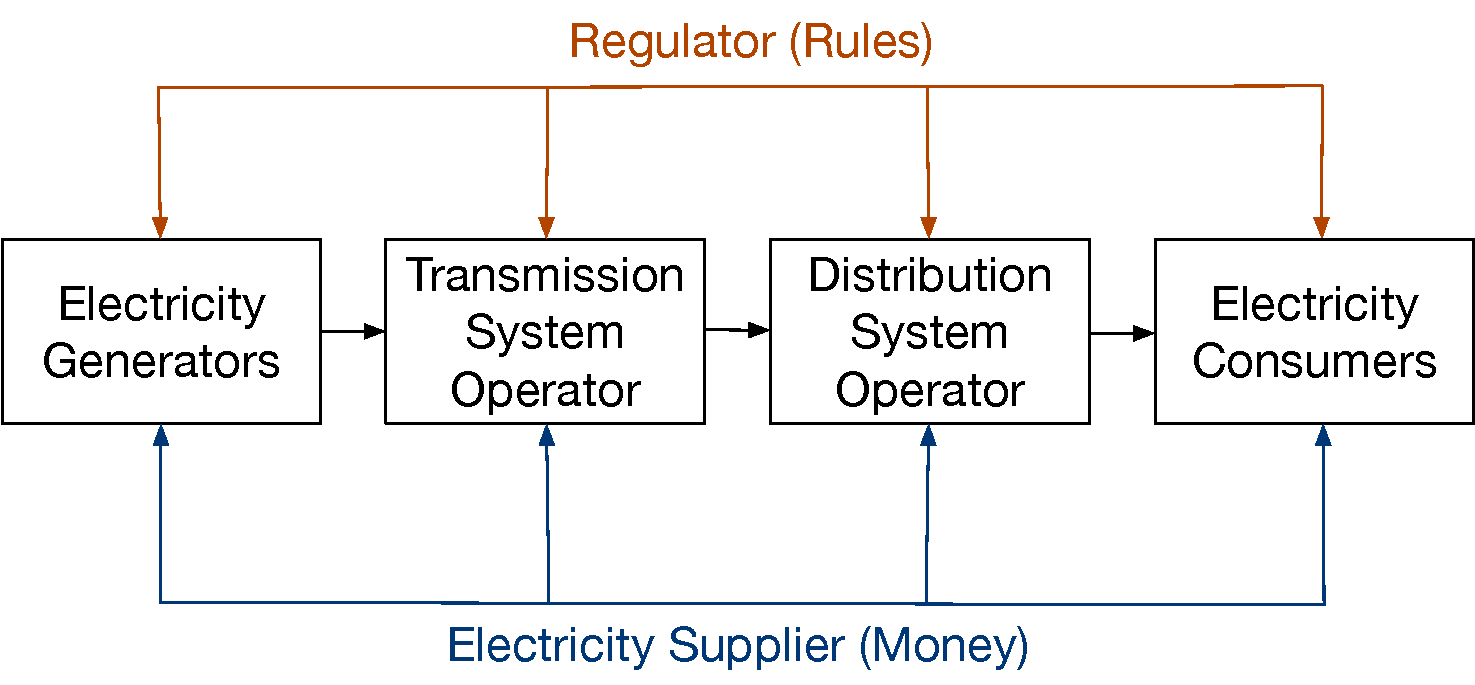
\includegraphics[width=0.9\linewidth]{figures/main_electricty_players}
% \caption{{\color{red}Schematic overview of the electricity system \cite{Erbach2016}.}}
% \label{fig:mainelectrictyplayers}
% \end{figure}

%%%%%%%%%%%%%%%%%%%%%%%%%%%%%%%%%%%%%%%%%%%%%%%%
%%%%%%%%%%%%%%%%%%%%%%%%      Paper 2    %%%%%%%%%%%%%%%%
%%%%%%%%%%%%%%%%%%%%%%%%%%%%%%%%%%%%%%%%%%%%%%%%

Optimization based solutions are the dominant approach for analysing energy policy \cite{Chappin2017}. However, the results of these models should be interpreted in a normative manner. For example, how investment and policy choices should be carried out, under certain assumptions and scenarios. The processes which emerge from an equilibrium model remain a black-box, making it difficult to fully understand the underlying dynamics of the model \cite{Chappin2017}. 



In addition to this, optimization models do not allow for  endogenous behaviour to emerge from typical market movements, such as investment cycles \cite{Chappin2017, Gross2007}. By modelling these naturally occurring behaviours, policy can be designed that is robust against movements away from the optimum/equilibrium. Thus, helping policy to become more effective in the real world. 

Agent-based models differ from optimization models by the fact that they are able to explore `\textit{what-if}' questions regarding how a sector could develop under different prospective policies, as opposed to determining optimal trajectories. \acrshort{abm}s are particularly pertinent in decentralised electricity markets, where a centralised actor does not dictate investments made within the electricity sector. \acrshort{abm}s have the ability to closely mimic the real world by, for example, modelling irrational agents, in this case Generation Companies (GenCos) with incomplete information in uncertain situations \cite{Ghorbani2014}. 


To further enhance the perfomance of ElecSim, we use representative days to model a year time period. Similarly to Nahmmacher \textit{et al.} we demonstrate how clustering of multiple relevant time series such as electricity demand, solar irradiance and wind speed can reduce computational time by selecting representative days ~\cite{Nahmmacher2016}. In this context, representative days are a subset of days that have been chosen due to their ability to approximate the weather and electricity demand in an entire year. Similarly to Nahmacher \textit{et al.} we use a Ward hierarchical clustering algorithm  \cite{doi:10.1080/01621459.1963.10500845}, However, we also try a $k$-means clustering approach \cite{forgy65}. We chose the $k$-means clustering approach due to previous success of this technique in clustering time series \cite{Kell2018a}. 



\subsection{Validation of long-term models}

There is a desire to validate the ability of energy-models to make long-term predictions. Validation increases confidence in the outputs of a model and leads to an increase in trust amongst the public and policy makers. Energy models, however, are frequently criticised for being insufficiently validated, with the performance of models rarely checked against historical outcomes \cite{Beckman2011}.

In answer to this, we postulate that \acrshort{abm}s can provide accurate information to decision makers in the context of electricity markets. We increase the temporal granularity of the work by Kell \textit{et al.} \cite{Kell} and use genetic algorithms to tune the model to observed data enabling us to perform validation. This enables us to understand the parameters required to observe certain phenomena, as well as use these fitted parameters to make inferences about the future. 


%- A short description of the solution


We use a genetic algorithm approach to find an optimal set of price curves predicted by generation companies (GenCos) that adequately model observed investment behaviour in the real-life electricity market in the United Kingdom. Similar techniques can be employed for other countries of various sizes \cite{Kell}. 

We measure the accuracy of projections for our improved \acrshort{abm} with those of the UK Government's Department for Business, Energy and Industrial Strategy (BEIS) for the UK electricity market between 2013 and 2018. In addition to this, we compare our projections from 2018 to 2035 to those made by BEIS in 2018 \cite{DBEIS2019}.




\subsection{Results}
\label{elecsim:sec:results}

Through this validation process, we are able to adequately model the transitional dynamics of the electricity mix in the United Kingdom between 2013 and 2018. During this time there was an ${\sim}88\%$ drop in coal use, ${\sim}44\%$ increase in Combined Cycle Gas Turbines (CCGT), ${\sim}111\% $ increase in wind energy and increase in solar from near zero to ${\sim}1250$MW. We are therefore able to test our model in a transition of sufficient magnitude.

%- What are the key take-home messages

We show in this Chapter, that agent-based models are able to mimic the behaviour of the UK electricity market under the same specific scenario conditions. Concretely, we show that under an observed carbon tax strategy, fuel price and electricity demand scenario, the model, ElecSim, closely matches the observed electricity mix between 2013 and 2018. We achieve this by determining an exogenous predicted price duration curve using a genetic algorithm to minimise error between observed and simulated electricity mix in 2018. The predicted price curve is an arrangement of all price levels in descending order of magnitude. The predicted price duration curve achieved is similar to that of the simulated price duration curve in 2018, increasing confidence in the underlying dynamics of our model. 

In addition, we compare our projections to those of the BEIS reference scenario from 2018 to 2035~\cite{DBEIS2019}. To achieve this, we use the same genetic algorithm optimisation technique as during our validation stage, optimising for predicted price duration curves. Our model demonstrates that we are able to closely match the projections of BEIS by finding a set of realistic price duration curves which are subject to investment cycles. Our model, however, exhibits a more realistic step change in nuclear output than that of BEIS. This is because, whilst BEIS projects a gradual increase in nuclear output, our model projects that nuclear output will grow instantaneously at a single point in time as a new nuclear power plant comes online. 

This allows us to verify the scenarios of other models, in this case BEIS' reference scenario, by ascertaining whether the optimal parameters required to achieve such scenarios are realistic. In addition to this, we are able to use these parameters to analyse `\textit{what-if}' questions with further accuracy.


\subsection{Contributions of this Chapter}
%- What are the key contributions

As part of this work we contribute a validated open-source agent-based model called ElecSim. Whilst we have used the United Kingdom as a use-case for this thesis, ElecSim is able to model decentralised markets of various sizes. 

To improve our results, we increased the temporal granularity of the model using a $k$-means clustering approach to select a subset of representative days for wind speed, solar irradiance and electricity demand. This subset of representative days enabled us to approximate an entire year and only required a fraction of the total time-steps that would be necessary to model each day of a year independently. This enabled us to decrease execution time. We show that we are able to provide an accurate framework, through this addition, to allow policy makers, decision makers and the public to explore the effects of policy on investment in electricity generators. 

We demonstrate that with a genetic algorithm approach we are able to optimise parameters to improve the accuracy of our model. Namely, we optimise the predicted electricity price, the uncertainty of this electricity price and nuclear subsidy. We validate our model using the observed electricity mix between 2013-2018.

A major contribution of this work is to demonstrate that it is possible for agent-based models to accurately model transitions in the UK electricity market. This was achieved by comparing our simulated electricity mix to the observed electricity mix between 2013 and 2018. In this time a transition from coal to natural gas was observed. We demonstrate that a high temporal granularity is required to accurately model fluctuations in wind and solar irradiance for intermittent renewable energy sources.


\clearpage
\section{Literature Review}
\label{elecsim:sec:litreview}

Whilst Chapter \ref{chapter:litreview} provided a review of the literature of models, this section covers the difficulties inherent in validating energy models and the approaches taken in the literature to validate these models..

\subsection{Limits of Validating Energy Models}

Beckman \textit{et al.} state that questions frequently arise as to how much faith one can put in energy model results. This is due to the fact that the performance of these models as a whole are rarely checked against historical outcomes~\cite{Beckman2011}.


Under the definition by Hodges \textit{et al.} \cite{Hodges} long-range energy forecasts are not validatable \cite{Craig2002}. Under this definition, validatable models must be observable, exhibit constancy of structure in time, exhibit constancy across variations in conditions not specified in the model and it must be possible to collect ample data \cite{Hodges}.


Whilst it is possible to collect data for energy models, the data covering important characteristics of energy markets are not always measured. Furthermore, the behaviour of the human population and innovation are neither constant nor entirely predictable. This leads to the fact that static models cannot keep pace with global long-term evolution. Assumptions made by the modeller may be challenged in the form of unpredictable events, such as the oil shock of 1973 \cite{Craig2002}.

This, however, does not mean that energy-modelling is not useful for providing advice in the present. A model may fail at predicting the long-term future because it has forecast an undesirable event, which led to a pre-emptive change in human behaviour. Thus avoiding the original scenario that was predicted. This could, therefore, be viewed as a success of the model.

Schurr \textit{et al.} argued against predicting too far ahead in energy modelling due to the uncertainties involved \cite{Schurr_1961}. However, they specify that long-term energy forecasting is useful to provide basic information on energy consumption and availability which is helpful in public debate and in guiding policy makers.


Ascher concurs with this view and states that the most significant factor in model accuracy is the time horizon of the forecast; the more distant the forecast target the less accurate the model. This can be due to unforeseen changes in society as a whole ~\cite{gillespie_1979}.

It is for these reasons that we focus on a shorter-term (5-year) horizon window when validating our model. This enables us to have an increased confidence that the dynamics of the model work without external shocks and can provide descriptive advice to stakeholders. However, it must be noted that the UK electricity market exhibited a fundamental transition from natural gas to coal electricity generation during this period, meaning that a simple data-driven modelling approach would not work.

In addition to this short-term cross-validation, we compare our long-term projections to those of BEIS from 2018 to 2035. It is possible that our projections and those of BEIS could be wrong, however, this allows us to thoroughly test a particular scenario with different modelling approaches, and allow for the possibility to identify potential flaws in the models.


\subsection{Validation Examples}

In this section we explore a variety of approaches used in the literature for energy model validation.

The model OSeMOSYS \cite{Howells2011} is validated against the similar model MARKAL\slash TIMES through the use of a case study named UTOPIA. UTOPIA is a simple test energy system bundled with ANSWER, a graphical user interface packaged with the MARKAL model generator \cite{Hunter2013, Noble2004}. Hunter \textit{et al.} use the same case study to validate their model Temoa \cite{Hunter2013}. In these cases, MARKAL\slash TIMES is seen as the "gold standard". In this paper, however, we argue that the ultimate gold standard should be real-world observations, as opposed to a hypothetical scenario.

The model PowerACE demonstrates that realistic prices are achieved by their modelling approach, however, they do not indicate success in modelling GenCo investment over a prolonged time period \cite{Ringler2012}.

Barazza \textit{et al}. validate their model, BRAIN-Energy, by comparing their results with a few years of historical data, however, they do not compare the simulated and observed electricity mix \cite{Barazza2020}.

Work by Koomey \textit{et al.} expresses the importance of conducting retrospective studies to help improve models \cite{Koomey2003}. In this case, a model can be rerun using historical data in order to determine how much of the error in the original forecast resulted from structural problems in the model itself, or how much of the error was due to incorrect specification of the fundamental drivers of the forecast \cite{Koomey2003}.

A retrospective study published in 2002 by Craig \textit{et al.} focused on the ability of forecasters to accurately predict electricity demand from the 1970s \cite{Craig2002}. They found that actual energy usage in 2000 was at the very lowest end of the forecasts, with only a single exception. They found that these forecasts underestimated unmodelled shocks such as the oil crises which led to an increase in energy efficiency.

Hoffman \textit{et al.} also developed a retrospective validation of a predecessor of the current MARKAL\slash TIMES model, named Reference Energy System \cite{Hoffman_1973}, and the Brookhaven Energy System Optimization Model \cite{ERDA_48}. These were studies applied in the 70s and 80s to develop projections to the year 2000. This study found that the models had the ability to be descriptive, but were not entirely accurate in terms of predictive ability. They found that emergent behaviours in response to policy had a strong impact on forecasting accuracy. The study concluded that forecasts must be expressed in highly conditioned terms \cite{Hoffman2011}. 




















\clearpage
\section{Architecture}
\label{elecsim:sec:architecture}

In this section we detail the architecture of how ElecSim has been designed.

ElecSim is made up of six parts: the agents, which are split up into demand and GenCos; power plants; a Power Exchange, which controls an electricity spot market; the time-steps ;and the data for parametrisation. A schematic of ElecSim is displayed in Figure \ref{fig:systemoverview}.

\begin{figure}
	\centering
	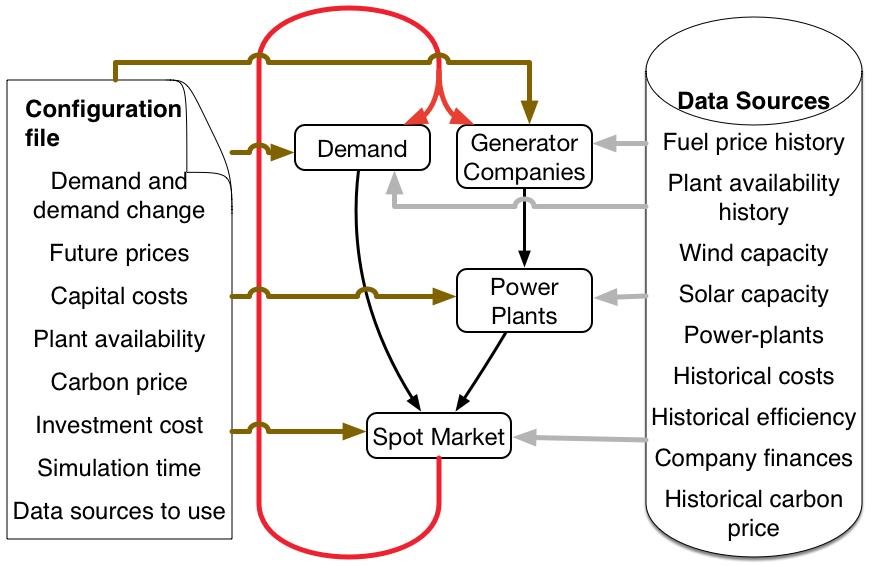
\includegraphics[width=0.85\linewidth]{Chapter4/figures/System_overview_large.png}
	\caption{High level overview.}
	\label{fig:systemoverview}
\end{figure}

\paragraph{Data parametrisation.} ElecSim contains a configuration file and a collection of data sources for parametrisation. These data sources contain information such as historical fuel prices, historical plant availability, wind and solar capacity.

The configuration file allows for rapid changes to test different hypothesis and scenarios, and points to the different data sources. The configuration file enables one to change the demand growth and shape, future fuel and carbon prices, capital costs, plant availability, investment costs and simulation time.

\paragraph{Demand Agent.} The demand agent is a simplified representation of aggregated demand in a country. The demand is represented as a load duration curve (LDC). An example load duration curve for a year is demonstrated in Figure \ref{fig:loaddurationcurve}. An LDC is an arrangement of all load levels in descending order of magnitude. where the lowest segment demand demonstrates baseload, and the highest segment represents peak demand. Each year, the demand agent changes each of the LDC segments proportionally.

 \begin{figure}
 	\centering
 	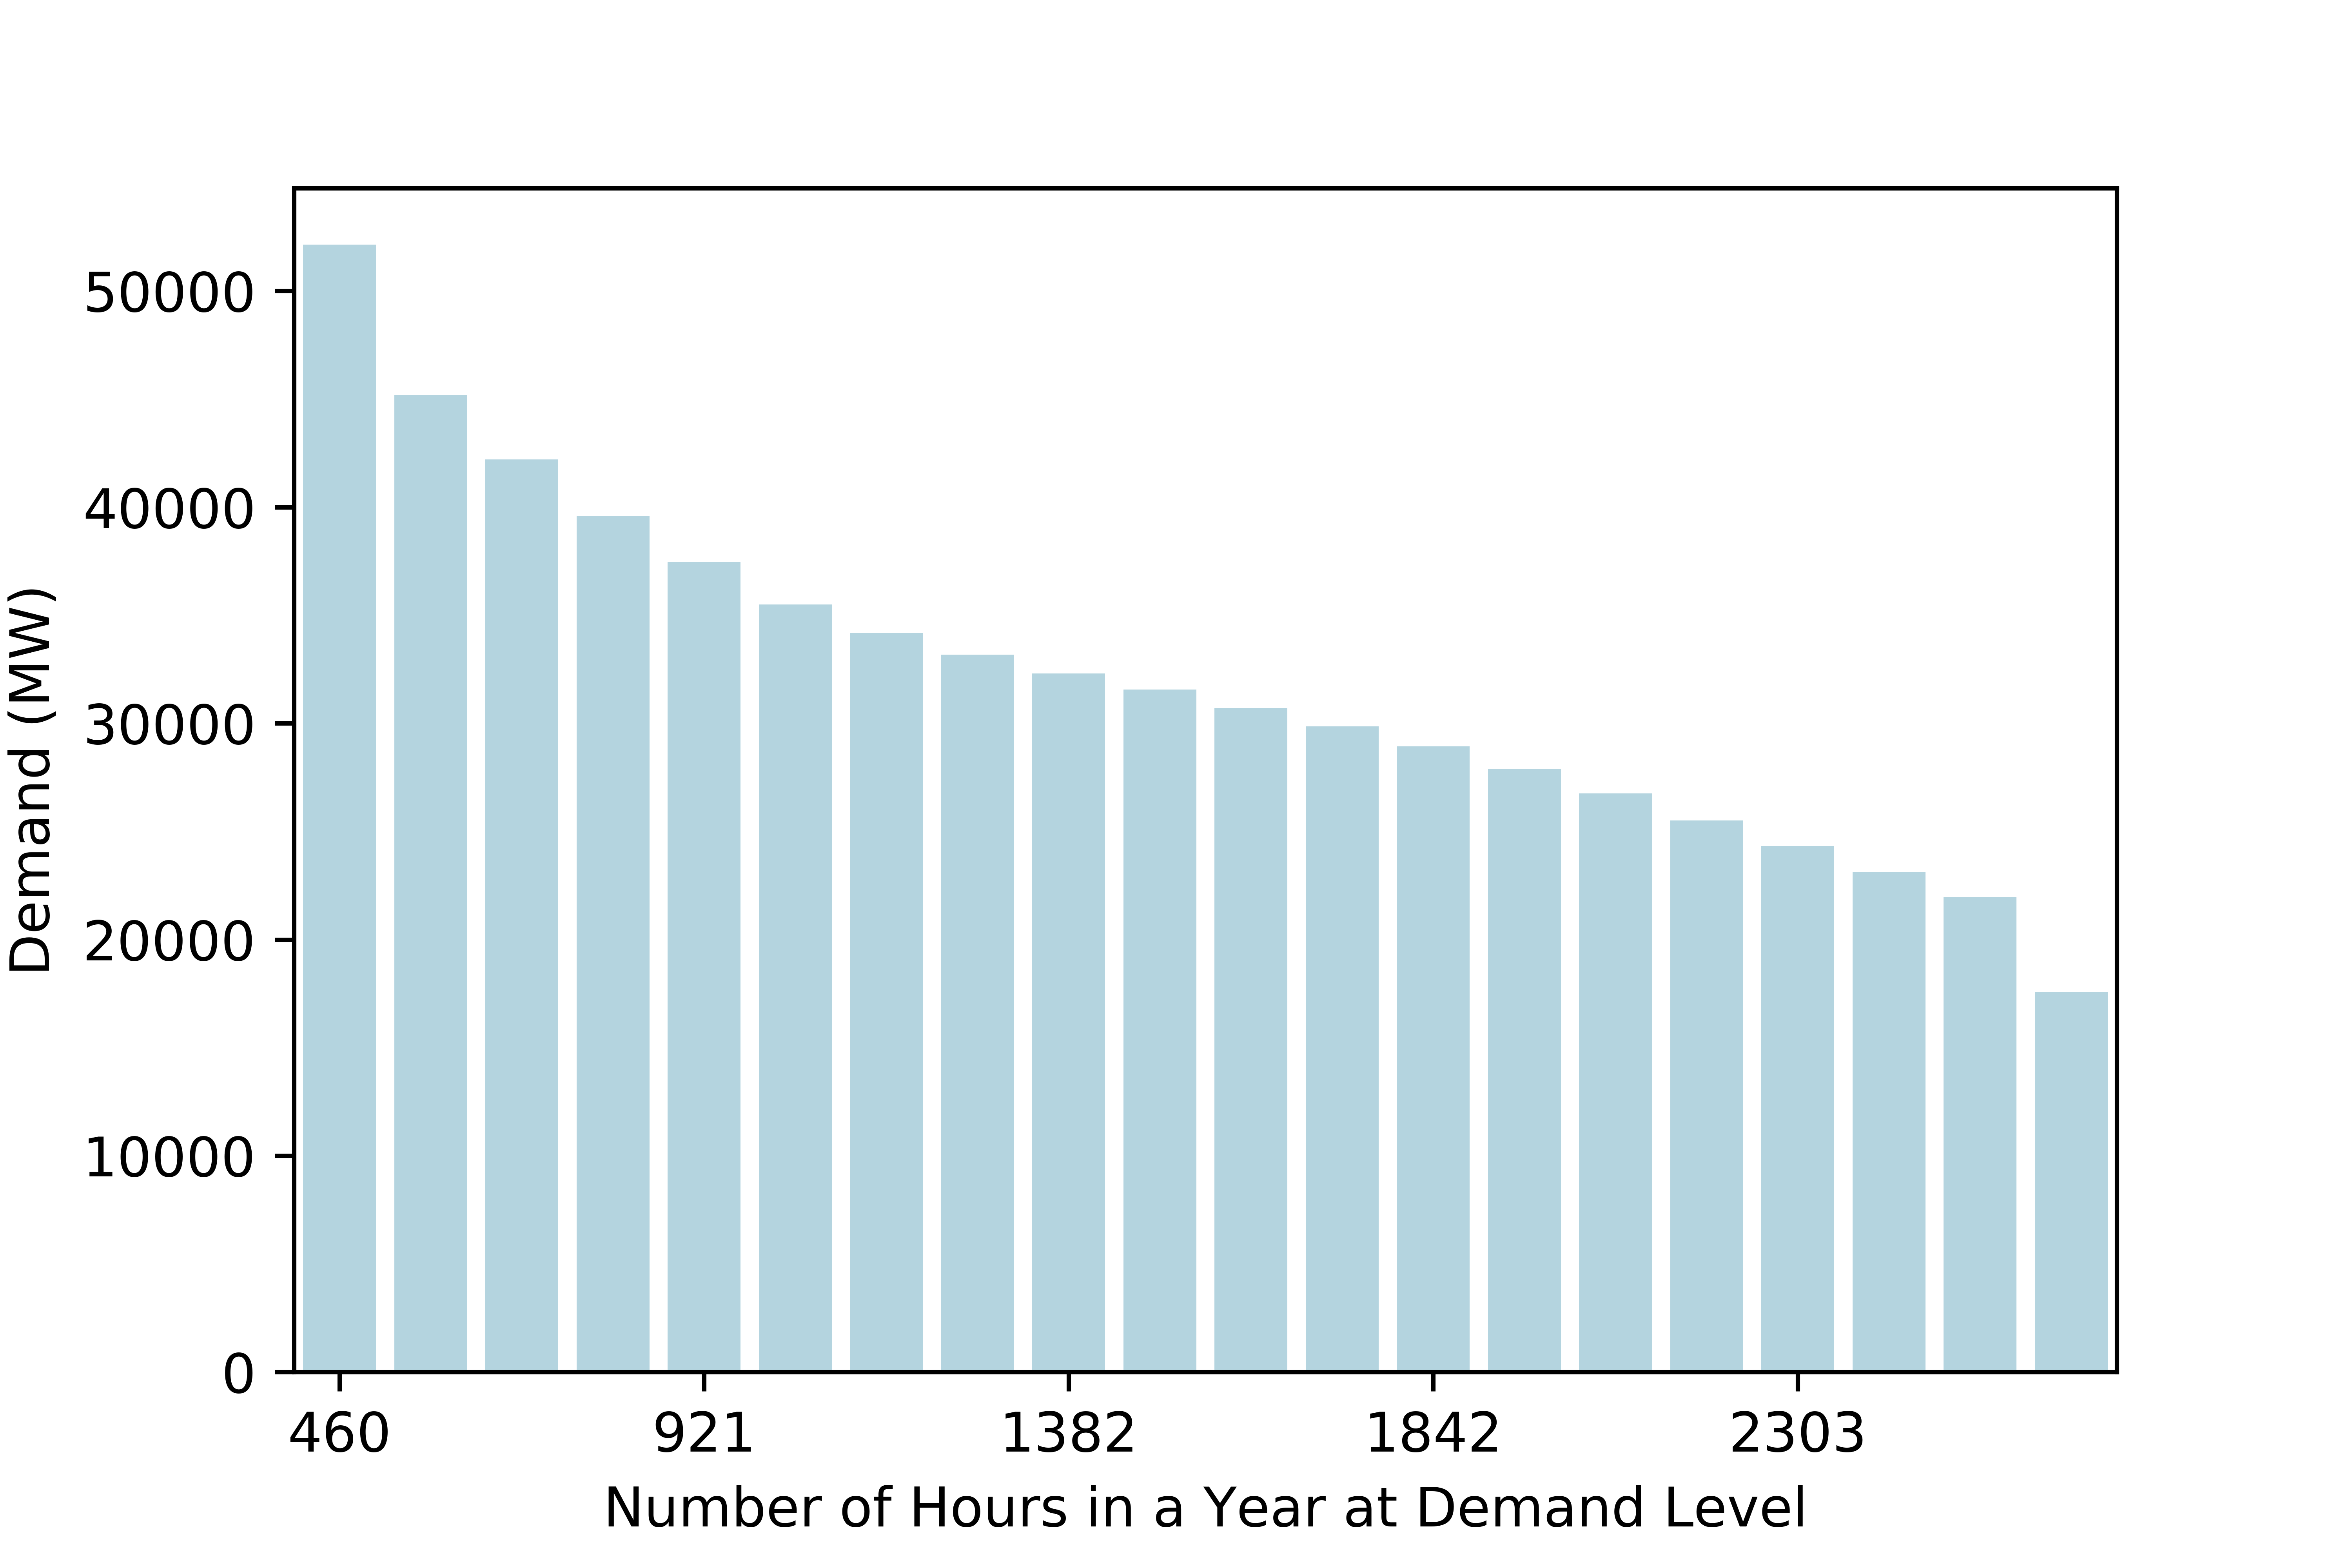
\includegraphics[width=0.95\linewidth]{Chapter4/figures/load_duration_curve}
 	\caption{Example load duration curve in a single year.}
  	\label{fig:loaddurationcurve}
 \end{figure}

%As per Chappin \textit{et al.} \cite{Chappin2017}, we modelled the LDC of electricity demand with twenty segments. Twenty segments enabled us to capture the variation in demand throughout the year to a high degree of accuracy, whilst reducing computational complexity. 


\paragraph{Generation Company Agents.} The GenCos have two main functions. Investing in power plants and making bids to sell their generation capacity. We will first focus on the buying and selling of electricity, and then cover the investment algorithm.

The power exchange runs every year, accepting the lowest bids until supply meets demand. Once this condition is met, the spot price or system marginal price (SMP) is paid to all generators regardless of their initial bid. Generators are motivated to bid their SRMC, to ensure that their generator is being utilised, and reduce the risk of overbidding.

\paragraph{Investment.} Investment in power plants is made based upon a net present value (NPV) calculation. NPV is a summation of the present value of a series of present and future cash flow. NPV provides a method for evaluating and comparing investments with cash flows spread over many years, making it suited for evaluating power plants which have a long lifetime.  \vphantom{\color{red}NPV is based upon the fact that current cash flow is worth more than future cash flow. This is due to the fact that money today can be invested and have a rate of return. This means that, for example \$50,000 today is worth more than \$50,000 in 10 years time. The value in which future cash flow is worth less than present cash flow is discounted by the discount rate.}

Equation \ref{architecture:eq:npv_eq} is the calculation of NPV, where $t$ is the year of the cash flow, $i$ is the discount rate, $N$ is total number of periods, or lifetime of power plant, and $R_t$ is the net cash flow at time $t$.
\begin{equation} \label{architecture:eq:npv_eq}
NPV(t, N) = \sum_{t=0}^{N}\frac{R_t}{(1+t)^t}
\end{equation}
A discount rate set by a GenCo's weighted average cost of capital (WACC) is often used \cite{KincheloeStephenC1990TWAC}. WACC is the rate that a company is expected to pay on average for its stock and debt. Therefore to achieve a positive NPV, an income larger than the WACC is required. However, a higher WACC is often selected to adjust for varying risk profiles, opportunity costs and rates of return. To account for these differences we sample from a Gaussian distribution, giving us sufficient variance whilst deviating from the expected price.

To calculate the NPV, future market conditions must be considered. For this, each GenCo forecasts $N$ years into the future, which we assume is representative of the lifetime of the plant. As in the real world, GenCos have imperfect information, and therefore must forecast expected demand, fuel prices, carbon price and electricity sale price. This is achieved by fitting functions to historical data. Each GenCo is different in that they will use differing historical time periods of data for forecasting.

Fuel and carbon price are forecast using linear regression. Demand, however, is forecast using an exponential function, which considers compounded growth. Linear regression is used if an exponential function is found to be sub-optimal.

The forecasted electricity price $N$ years ahead is difficult to ascertain accurately. We therefore use two methods for forecasting these. The first is to simulate a market $N$ years ahead. The second is to optimise for the predicted PDC using a genetic algorithm. We describe this optimisation in Section \ref{architecture:sec:validation}.

For the simulated market, the forecasted data is used to simulate a market $N$ years into the future using the electricity market algorithm. We simulate a market based on the expected bids -- based on SRMC -- that every operating power plant will make. This includes the removal of plants that will be past their operating period, and the introduction of plants that are in construction or pre-development stages. 

There may be scenarios where demand is forecast to grow significantly, and limited investments have yet been made to meet that demand. The expected price, would be that of lost load. Lost load is defined as the price customers would be willing to pay to avoid disruption in their electricity supply. To avoid GenCos from estimating large profits, and under the assumption that further power plant investments will be made, the lost load price is replaced with a predicted electricity price using linear regression based on prices at lower points of the demand curve. If zero segments of demand are met, then the  lost load price is used to encourage investment. 

Once this data has been forecasted, the NPV can be calculated. GenCos must typically provide a certain percentage of upfront capital, with the rest coming from investors in the form of stock and shares or debt (WACC). The percentage of upfront capital can be customised by the user in the configuration file. The GenCos then invest in the power plants with the highest NPV. 


\paragraph{Time-steps} For the time-steps, two approaches were taken. For the first approach, as per Chappin \textit{et al.} \cite{Chappin2017}, we modelled the LDC of electricity demand with twenty segments. Twenty segments enabled us to capture the variation in demand throughout the year to a high degree of accuracy, whilst reducing computational complexity. However, as we show later in Section \ref{elecsim:sec:scenarios}, this led to an overestimation of the supply of \acrshort{ires}. 

For the second approach, we used representative days to model a year. Representative days in this context are a subset of days which have characteristics, that when scaled proportionally can accurately model an entire year. To select these representative days we used a $k$-means approach. We describe this in full detail in Section \ref{elecsim:sec:representative}



\paragraph{Power Plant Parameters.}\label{elecsim:ssssec:powerplantparameters} Costs form an important element of markets and investment, and publicly available data for power plant costs for individual countries can be scarce. Thus, extrapolation and interpolation is required to estimate costs for power plants of differing sizes, types and years of construction.

Users are able to initialise costs relevant to their particular country by providing detailed cost parameters. They can also provide an average cost per MWh produced over the lifetime of a plant, known as levelised cost of electricity (LCOE).

The parameters used to initialise the power plants are detailed in this section. Periods have units of years and costs in \textsterling/MW unless otherwise stated: Efficiency ($\eta$) is defined as the percentage of energy from fuel that is converted into electrical energy (\%). Operating period ($OP$) is the total period in which a power plant is in operation. Pre-development period ($P_D$) and pre-development costs ($P_C$) include the time and costs for pre-licensing, technical and design, as well as costs incurred due to regulatory, licensing and public enquiry. The construction period ($C_D$) and construction costs ($C_C$) are incurred during the development of the plant, excluding network connections. The infrastructure costs ($I_C$) are the costs incurred by the developer in connecting the plant to the electricity or gas grid (\textsterling). Fixed operation \& maintenance costs ($F_C$) are costs incurred in operating the plant that do not vary based on output. Variable operation \& maintenance ($V_C$) costs are incurred in operating the plant that depend on generator output \cite{Ltd2016}.



%\begin{table}[h]
%	\centering
%	\csvautobooktabular{tables/notation_formated.csv}
%	\caption{Parameter notation. (Whilst the unit of currency displayed is \textsterling, this can be modified to other currencies eg. \$, \texteuro)}
%	\label{table:parameter_notation}
%\end{table}
%\addtolength{\textfloatsep}{-0.2in}

Precise data is not available for every plant size. Linear interpolation is used to estimate individual prices between known points. When the plant to be estimated falls outside of the range of known data points, the closest power plant is used. We experimented with extrapolation but this would often lead to unrealistic costs. %{\color{red}For example, the parameters of a 1,500MW combined cycle gas plant (CCGT) are estimated to be the same as a 1,200MW CCGT plant if the 1,200MW plant was the largest available data point. }

If specific parameters are not known, the LCOE can be used for parameter estimation, through the use of linear optimisation. Constraints can be set by the user, enabling, for example, varying operation and maintenance costs per country as a fraction of LCOE.

To fully parametrise power plants, availability and capacity factors are required. Availability is the percentage of time that a power plant can produce electricity. This can be reduced by forced or planned outages. We integrate historical data to model improvements in reliability over time.

The capacity factor is the actual electrical energy produced over a given time period divided by the maximum possible electrical energy it could have produced. The capacity factor can be impacted by regulatory constraints, market forces and resource availability. For example, higher capacity factors are common for photovoltaics in the summer, and lower in winter. 

To model the intermittency of wind and solar power we allow them to contribute only a certain percentage of their total capacity (nameplate capacity) for each load segment. This percentage is based upon empirical wind and solar capacity factors. In this calculation we consider the correlation between demand and renewable resources. 

When initialised, $V_C$ is selected from a uniform distribution, with the ability for the user to set maximum percentage increase or decrease. A uniform distribution was chosen to capture the large deviations that can occur in $V_C$, especially over a long time period. \vphantom{By doing this, the variance in costs between individual power plants for processes such as preventative and corrective maintenance, labour costs and skill, health and safety and chance are different per plant instant.}

Fuel price is controlled by the user, however, there is inherent volatility in fuel price. To take into account this variability, an ARIMA \cite{ARIMA} model was fit to historical gas and coal price data. The standard deviation of the residuals was used to model the variance in price that a GenCo will buy fuel in a given year. This considers differences in chance and hedging strategies.


%\vphantom{With historical power plants which have been refurbished, we sample their initialisation randomly between 15 years prior to the initialisation year and the initialisation year. This is done because there is rarely a comprehensive data set on when plants are refurbished. 15 years was chosen due to the fact that plants often have an operating period of 25 years, and therefore 15 years allowed for sufficient variance in results, whilst keeping plants in operation.}

Figure \ref{fig:lowlevelsystem} demonstrates the simulation and how it co-ordinates runs. The world contains data and brings together GenCos, the Power Exchange and demand. The investment decisions are based on future demand and costs, which in turn influence bids made.

\begin{landscape}
	\begin{figure*}
		\centering
		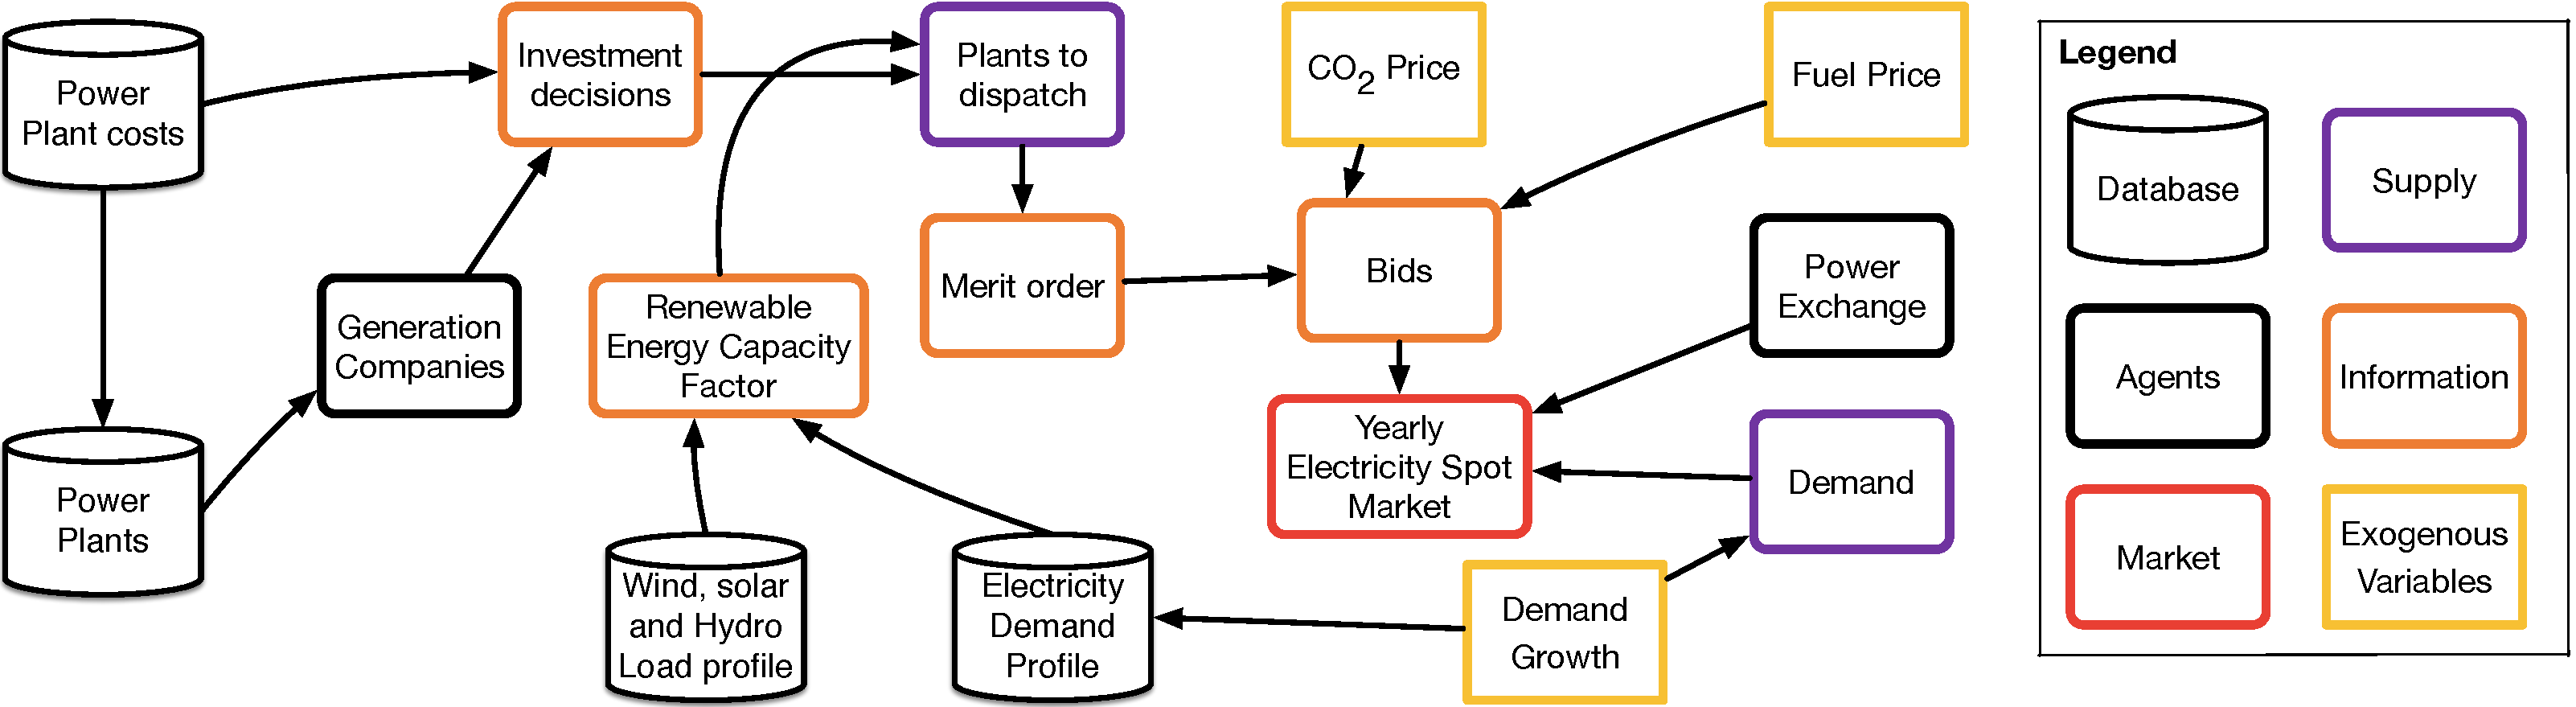
\includegraphics[width=\linewidth]{Chapter4/figures/low_level_system}
		\caption{ElecSim simulation overview}
		\label{fig:lowlevelsystem}
	\end{figure*}
\end{landscape}

Exogenous variables include fuel and \ce{CO2} prices as well as demand growth. Once the data is initialised, the world calls on the Power Exchange to operate the yearly electricity spot market. The world also settles the accounts of the GenCos, by paying bids, and removing operating and capital costs as well as loans and dividends.

%The world contains the functionality to dismantle old plants once they have reached the end of their lifetime. Power plants are taken out of service if they have not sold any electricity in the past 7 years, which is configurable in the configuration file. We decided upon this due to the fact that power generators have high, sunk capital costs, which often have high demolition costs. We assume, therefore, that generator companies are willing to wait circa $\frac{1}{4}$ of their lives to see if a pay-out occurs due to the breakdown of competing power plants, increasing demand, or governmental support in the form of a carbon tax increase or reduction.






%GenCos  invest in power plants based on the highest positive net present value (NPV). Bids are made for each power plant based on the power plants short run marginal cost. A Power Exchange operator matches these bids with demand in merit order. 



%\begin{figure}[h]
%	\begin{center}
%		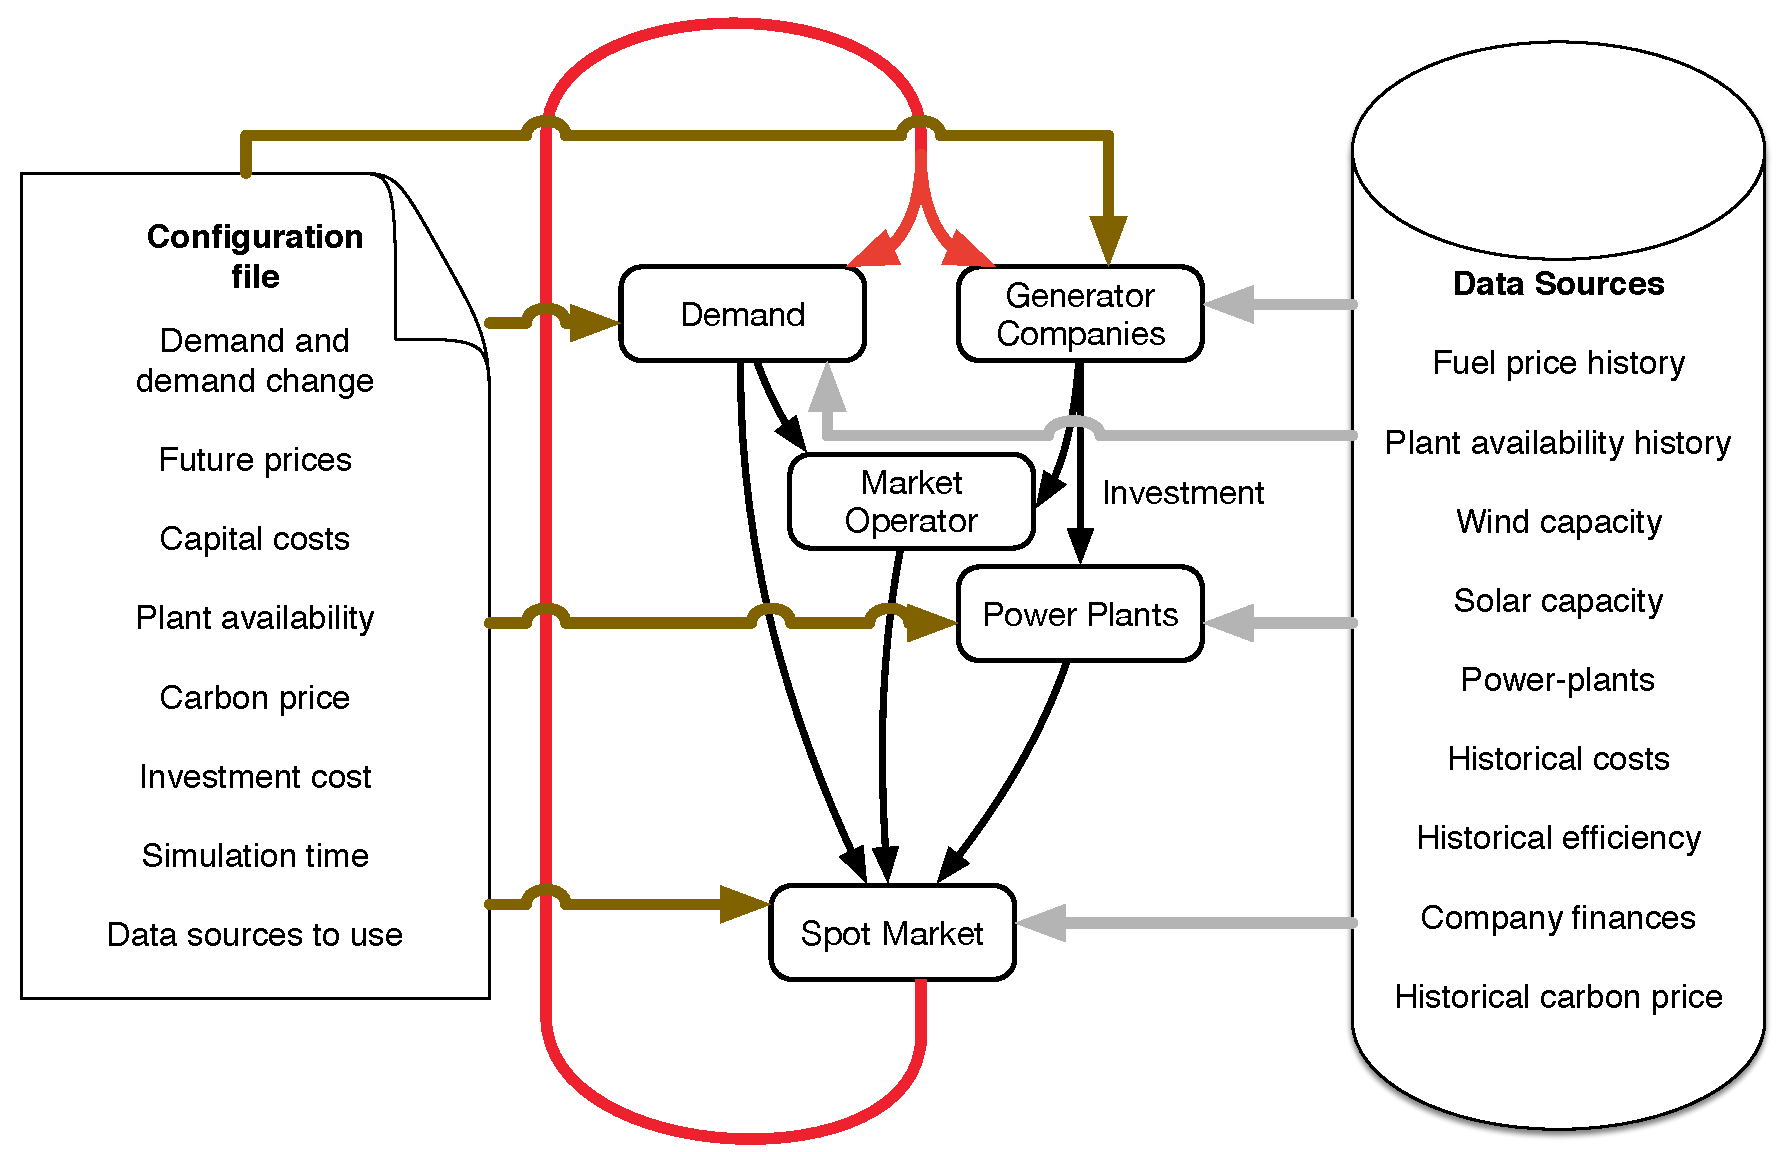
\includegraphics[width=0.5\textwidth]{figures/System_overview.pdf}
%		\caption{ElecSim simulation overview.}
%		\label{fig:system_overview}
%	\end{center}
%\end{figure}



% {\color{blue}
% \subsection{UK Case Study}

% Here we study a realisation of ElecSim, which we calibrated to the United Kingdom.

% \subsubsection{Exogenous Inputs}

% To model variance in gas and coal prices we used data from \cite{coalprices,gasprices}. Calibration of the load duration curve was taken from \cite{gbnationalgridstatus_2019}.

% Historical EU ETS carbon price was taken from \cite{jones_moore_macdonald_macdonald_buckley_macdonald_2019}. The EU ETS is the EU emissions trading scheme, which limits total carbon emissions within the EU area.

% \subsubsection{Power Plant Parameters}

% ElecSim's power generation costs are initialised using the UK government Department for Business, Energy and Industrial Strategy (BEIS) power plant generation report \cite{Department2016}. This contains information on power plants found in Table \ref{table:parameter_notation}.

% For historical power plants, we used historical costs of Levelised Cost of Energy (LCOE) \cite{Dale2013}, from the International Energy Agency and International Renewable Energy Agency energy cost reports, localised to the UK \cite{IEA2015,IRENA2018}. In this realisation, each parameter was scaled linearly going from the modern LCOE calculated from the BEIS report, to attain the relevant historical LCOE. Historical plant efficiency was taken into account for gas and coal power plants using data from the USA \cite{EIA2013}.

% Outages are modelled by using availability data of gas, coal, photovoltaic, offshore and onshore power generators \cite{Ltd2016, Hunt2015, carroll-j}. Historical availabilities are modelled for older gas, coal and hydro power plants \cite{AlbertaSystemElectricOperator2016}.

% Capacity factors were taken as an average of the UK for solar and wind \cite{Pfenninger2016, Staffell2016}.






% \subsubsection{Spot Market}

% The lost load is set to be \textsterling6000 to encourage investment as per the recommendations of the UK government \cite{DECC2013}.

% \subsubsection{Investment}

% As agents are modelled to have imperfect information, we model that they make predictions on future electricity and \ce{CO2} prices, as well as demand change. Each generation company has a different look-back period sampled uniformly from the previous 3 to 7 years.


% The cost of equity and debt is modelled as a weighted average cost of capital (WACC), with values of 5.9\% for non-nuclear power plants, and 10\% for nuclear power plants \cite{KPMG2017, Paper2012}. 

% }



%
%\begin{itemize}
%	\item Model can be modified through a single python scenario file which includes exogenous variables such as number of generation companies, power plants, power plant costs, tax and fuel prices, and demand.
%	\item Architectural framework:
%	\begin{itemize}
%		\item Agents are generation companies.
%		\item Generation companies initialized from government data. And randomized discount rate around a mean of 10\% for nuclear power plants and 5.9\% for other types of generators.
%		\item Costs of power plants taken from empirical data. 
%		\item Historical LCOE costs taken from data, with individual costs such as fixed operation and maintenance, construction and pre-development costs scaled linearly to match LCOE value. (This can be changed by user by specifying linear optimisation constraints).
%		\item Historical Gas turbine and Coal plant efficiency taken from epa data.
%		\item Variable operation and maintenance costs are stochastic to take into account differences in design types, preventative and corrective maintenance, labour costs and skill, asset and site management, health and safety and chance.
%		\item Electricity demand taken from historical data and split up into 19 load segments.
%		\item CO2 prices, fuel Prices, demand growth are exogenous
%		\item Fuel is bought by power producers each year at different prices, related to the standard deviation from historical data. This simulates different hedging strategies, luck and timing of fuel purchasing.
%		\item Outages are modelled by assuming a 93\% outage rate for fuel plants \cite{Ltd2016} and 97\% outage for renewables. \cite{carroll-j}
%		\item Generation companies bid their short run marginal costs.
%		\item Investments made on highest Net Present Value results. CO2 price, fuel price and demand are predicted 7 years ahead using linear regression. 
%		\item Estimated sale of electricity price calculated by simulating a market 7 years into the future with expected power plants that are running and have been taken out of service.
%		\item Investors will only invest if they have 25\% of the total upfront costs. (the rest taken on by debt and equity as assumed by WACC value.)
%		\item Intermittent power generators can only submit a certain percentage of their total capacity for each load segment. This percentage is matched with empirical data.
%		\item Bids accepted by a centralised Power Exchange based on merit order. Generation companies bid their short run marginal cost.
%	\end{itemize}
%	\item Assumptions: 
%	\begin{itemize}
%		\item Yearly time step
%		\item Renewables contribute to load curve of each demand segment matched with empirical data of typical wind and solar availability at each demand segment
%		\item Different discount rates per user (randomized)
%		\item Country initialized with full amount of power plants and generation companies in country and total demand data considered
%		\item No curtailment of renewables
%		\item Imperfect foresight - Prediction required for demand, co2 price, fuel cost, other investments.
%		\item Power plant construction and pre-development periods and costs modelled from UK Government BEIS data
%		\item Investments based on highest NPV using a single year 7 (can be changed in scenario file) time steps into the future to predict all years of power plant.
%		\item Agents predict next year's fuel, carbon and demand using linear regression and randomized look back period (between 3 and 6.)
%		\item Plants are dismantled after their lifetime, and only enter operation after pre-development/construction.
%		\item Legacy power plants are reinitialized to random starting year to account for refurbishment.
%		\end{itemize}
%\end{itemize}


%%%%%%%%%%%%%%%%%%%%%%%%%%%%%%%%%%%%%%%%%%%%%%%%
%%%%%%%%%%%%%%%%%%%%%%%%     Poster    %%%%%%%%%%%%%%%%
%%%%%%%%%%%%%%%%%%%%%%%%%%%%%%%%%%%%%%%%%%%%%%%%



We initialise the United Kingdom with our model with exemplar data from the UK. We model every single power plant in operation in the year 2018, which are owned by their respective generation companies. Individual historical power plant costs are estimated from levelized cost of electricity (LCOE) \cite{Dale2013, IEA2015,IRENA2018}, whereas future and present power plant costs are taken from the department of business and industrial strategy \cite{Department2016}. The variable operation and maintenance cost was defined stochastically to model the varying costs per project. A uniform distribution was chosen to provide sufficient variance between projects.

The demand agent is modelled as a single aggregated demand, split up into 20 segments of a yearly load duration curve (LDC), enabling us to increase speed of computation whilst maintaining accuracy. An LDC is defined as load sorted in order of magnitude. 

We model the influence of outages using availability data for gas, coal, photovoltaic, and wind power generators \cite{Ltd2016, Hunt2015, carroll-j}. Historical availabilities are modelled for old gas, coal and hydro power plants \cite{AlbertaSystemElectricOperator2016}. Capacity factors per geographical location were taken as an average of the UK for solar and wind \cite{Pfenninger2016, Staffell2016}. Where a capacity factor is defined as the ratio of electrical output over a given time period over the maximum possible electrical energy output. 

The generation companies make electricity bids each year for each of their power plants. The market operator then matches demand with supply in order of price, also known as merit-order dispatch. We model a uniform pricing market, where each of the companies are paid the highest accepted bid per load segment.

GenCos have the ability to invest every year in new power plants based on the expected net present value (NPV) of each type of power plant. NPV is a summation of the present value of a series of present and future cash flow. The NPV calculation is dependent on a stochastic representation of GenCos predictions of fuel, carbon and electricity price and demand.

Each GenCo has a separate weighted average cost of capital (WACC), which is the average rate that a company is expected to for its stock and debt. This is used as the discount rate in the NPV calculation \cite{KincheloeStephenC1990TWAC}. The WACC is modelled as a stochastic variable, with a Gaussian distribution, with a $\pm3\%$ standard deviation, with values of 5.9\% for non-nuclear power plants, and 10\% for nuclear power plants \cite{KPMG2017, Paper2012}. 

Stochasticity of fuel price within a year was also modelled, to take into account difference in hedging strategies and chance. An ARIMA model \cite{ARIMA} was fit to historic coal and natural gas prices.



%%%%%%%%%%%%%%%%%%%%%%%%%%%%%%%%%%%%%%%%%%%%%%%%
%%%%%%%%%%%%%%%%%%%%%%%%      Paper 2    %%%%%%%%%%%%%%%%
%%%%%%%%%%%%%%%%%%%%%%%%%%%%%%%%%%%%%%%%%%%%%%%%

\subsection{Representative days}
\label{elecsim:sec:representative}


In this subsection we describe how we decide the granularity of time-steps. Specifically, we use representative days. Representative days, in this context, are a subset of days which when scaled up to 365 days can adequately represent a year. 

In this paper, we initialised the model to a scenario of the United Kingdom as an example, however, the fundamental dynamics of the model remain the same for other decentralised electricity markets.


%\subsection{Representative Days}
%\label{ssec:representative_days}

%In previously published work, ElecSim modelled a single year as 20 time-steps for solar irradiance, onshore and offshore wind and electricity demand~\cite{Kell}. Similarly to findings of other authors, this relatively low number of time-steps led to an overestimation of the uptake of intermittent renewable energy resources (IRES) and an underestimation of flexible technologies~\cite{Ludig2011,Haydt2011}. This is due to the fact that the full intermittent nature of renewable energy could not be accurately modelled in such a small number of time-steps.



Similarly to findings of other authors, using a relatively low number of time-steps leads to an overestimation of the uptake of intermittent renewable energy resources (IRES) and an underestimation of flexible technologies~\cite{Ludig2011,Haydt2011}. This is due to the fact that the full intermittent nature of renewable energy could not be accurately modelled in such a small number of time-steps. 


To address this problem, whilst maintaining a tractable execution time, we approximated a single year as a subset of proportionally weighted, representative days. This enabled us to reduce computation time. Each representative day consisted of 24 equally separated time-steps, which model hours in a day. Hourly data was chosen, as this was the highest resolution of the dataset available for offshore and  onshore wind and solar irradiance \cite{Pfenninger2016}. A lower resolution would allow us to model more days, however, we would lose accuracy in terms of the variability of the renewable energy sources. 


Similarly to Nahmmacher \textit{et al.} we used a clustering technique to split similar days of weather and electricity demand into separate groups. We then selected the historic day that was closest to the centre of the cluster, known as the medoid, as well as the average of the centre, known as the centroid ~\cite{Nahmmacher2016}. Similarly to Nahmmacher, we used Ward's clustering algorithm and selected the centroid \cite{doi:10.1080/01621459.1963.10500845}. However, we also used the $k$-means clustering algorithm~\cite{forgy65}. This was due to the ability for the $k$-means algorithm to cluster time-series into relevant groups \cite{Kell2018}. These days were scaled proportionally to the number of days within their respective cluster to approximate a total of 365 days. The Ward's clustering algorithm is an extension of the work published in \cite{Kell2020}

Equation \ref{elecsim:eq:medoids_series} shows the series for a medoid or centroid, selected by the clustering algorithms:

\begin{equation}
\label{elecsim:eq:medoids_series}
P^{x,i}_{h}=\{P_1, P_2, \ldots, P_{24}\}
\end{equation}

\noindent where $P^{x,i}_{h}$ is the medoid for series $x$, where $x\in X$ refers to offshore wind capacity factor, onshore wind capacity factor, solar capacity factor and electricity demand, $h$ is the hour of the day and $i$ is the respective cluster. $\{P_1, P_2, \ldots , P_{24}\}$ refers to the capacity values at each hour of the representative day.

We then calculated the weight of each cluster. This gave us a method of assigning the relative importance of each representative day when scaling the representative days up to a year. The weight is calculated by the proportion of days in each cluster. This gives us a method of determining how many days within a year are similar to the selected medoid or centroid. The calculation for the weight of each cluster is shown by Equation \ref{elecsim:eq:cluster_weight}:

\begin{equation}
\label{elecsim:eq:cluster_weight}
w_i = \frac{n_i}{||N||} 
\end{equation} 

\noindent where $w_i$ is the weight of cluster $i$, $n_i$ is the number of days in cluster $i$, and $||N||$ is the total number of days that have been used for clustering. 


The next step was to scale up the representative days to represent the duration curve of a full year. We achieved this by using the weight of each cluster, $w_i$, to increase the number of hours that each capacity factor contributed in a full year. Equation \ref{elecsim:eq:scaled-medoid} details the scaling process to turn the medoid or centroid, shown in Equation \ref{elecsim:eq:medoids_series}, into a scaled day. Where $\widetilde{P}^{x,i}_{h}$ is the scaled day:

\begin{equation}
\label{elecsim:eq:scaled-medoid}
\widetilde{P}^{x,i}_{h} =  \{P_{1w_i}, P_{2w_i}, \ldots, P_{24w_i}\}
\end{equation} 

\noindent Equation \ref{elecsim:eq:scaled-medoid} effectively extends the length of the day proportional to the amount of days in the respective cluster.


%The total time series for series $x$ is shown by Equation \ref{eq:total_time_series}

Finally, each of the scaled representative days were concatenated to create the series used for the calculations which required the capacity factors and the respective number of hours that each capacity factor contributed to the year. Equation \ref{elecsim:eq:total_time_series} displays the total time series for series $x$, where each scaled medoid is concatenated to produce an approximated time series, $\widetilde{P}^x$:


\begin{equation}
\label{elecsim:eq:total_time_series}
\widetilde{P}^x=\left(\widetilde{P}^{x,1}_{h},\widetilde{P}^{x,2}_{h},\ldots, \widetilde{P}^{x,||N||}_{h}\right)
\end{equation}

\noindent the total number of hours in the approximated time series, $\widetilde{P}^x$, is equal to the number of hours in a day multiplied by the number of days in a year, which gives the total number of hours in a year ($24\times 365=8760$), as shown by Equation \ref{elecsim:eq:total_scale}:


\begin{equation}
\label{elecsim:total_scale}
\sum\limits_{w\in W}\sum\limits_{t=1}^{T=24}\left(w_i t\right)=24\times 365=8760
\end{equation}

\noindent where $w\in W$ is the set of clusters.

\subsection{Error Metrics}

To measure the validity of our approximation using representative days and also compare the optimum number of days, or clusters, we used a technique similar to Poncelet \textit{et al.} \cite{Dhaeseleer2015, Poncelet2017}. We trialled the number of clusters against three different metrics: correlation ($CE_{av}$), normalised root mean squared error ($nRMSE$) and relative energy error ($REE_{av}$). 

$REE_{av}$ is the average value over all the considered time series $\widetilde{P}^x{\in} \widetilde{P}$ compared to the observed average value of the set $P^x\in P$. Where $P^x\in P$ are the observed time series and $\widetilde{P}^x{\in} \widetilde{P}$ are the scaled, approximated time series using representative days. $REE_{av}$ is shown formally by Equation \ref{eq:ree_av}:


\begin{equation}
\label{eq:ree_av}
REE_{av}=\frac
{\sum\limits_{P^x{\in} P}\left(\left|
	\frac
	{\sum\limits_{t\in T}DC_{P^x_t}-\sum\limits_{t\in T}\widetilde{DC}_{\widetilde{P}^x_t}}
	{\sum\limits_{t\in T}DC_{P^x_t}}
	\right|\right)
}
{\left|\left|P\right|\right|}
\end{equation}

\noindent where $DC_{P^x_t}$ is the duration curve for $P^x$ and $DC_{\widetilde{P}^x_t}$ is the duration curve for $\widetilde{P}^x$. In this context, the duration curve can be constructed by sorting the capacity factor and electrical load data from high to low. The $x-$axis for the DC exhibits the proportion of time that each capacity factor represents. The approximation of the duration curve is represented in this text as $\widetilde{DC}_{\widetilde{p}^x}$.

$t\in T$ refers to a specific time step of the original time series. $\widetilde{DC}$ refers to the approximated duration curve for $\widetilde{P}^x$. Note that in this text $\left|\cdot\right|$ refers to the absolute value, and $\left|\left|\cdot\right|\right|$ refers to the cardinality of a set and $\left|\left|P\right|\right|$ refers to the total number of of considered time series.

Specifically, the sum of the observed values, $P^x$, and approximated values, $\widetilde P^x$, for all of the time series are summed. The proportional difference is found, which is summed for each of the different series, $x$, and divided by the number of series, to give $REE_{av}$.





%$nRMSE$ is measured as the normalised root mean squared error between the actual duration curve and representative duration curve, $DC$.  

%Another metric that we wanted to measure was that of the distribution of electricity demand and capacity factors to be similar to that of the actual time series. The distribution can be represented by a duration curve ($DC$) of the original time series. We therefore used the normalised root mean squared error between the actual duration curve and representative duration curve. 

Another requirement is for the distribution of load and capacity factors for the approximated series to correspond to the observed time series. It is crucial that we can account for both high and low levels of demand and capacity factor for IRES generation. This enables us to model for times where flexible generation capacity is required.

The distribution of values can be represented by the duration curve ($DC$) of the time series. Therefore, the average normalised root-mean-square error ($NRMSE_{av}$) between each $DC$ is used as an additional metric. The $NRMSE_{av}$ is shown formally by Equation \ref{eq:nrmse_av}:

\begin{equation}
\label{eq:nrmse_av}
NRMSE_{av}=\frac
{\sum\limits_{P^x{\in} P}\left(\frac
	{\sqrt{
			\frac{1}{\left|\left|T\right|\right|}
			\cdot
			\sum\limits_{t\in T}(DC_{P^x_t}-\widetilde{DC}_{\widetilde{P}^x_t})^2}
	}
	{max(DC_{P^x})-min(DC_{P^x})}
	\right)}
{\left|\left|P\right|\right|}.
\end{equation}

Specifically, the difference between the approximated and observed duration curves for each time-step $t$ is calculated. The average value is then taken of these differences. This average value is then normalised for the respective time series $P^x$. The average of these average normalised values for each time series are then taken to provide a single metric, $NRMSE_{av}$.



The final metric used is the correlation between the different time series. This is used due to the fact that wind and solar output influences the load within a single region, solar and wind output are correlated, as well as offshore and onshore wind levels within the UK. This is referred to as the average correlation error ($CE_{av}$) and shown formally by Equation \ref{eq:ce_av}:


\begin{equation}
\label{eq:ce_av}
CE_{av}=\frac{2}{\left|\left|P\right|\right|\cdot(\left|\left|P\right|\right|-1)}\cdot
\left(
\sum\limits_{p_i\in P}\sum\limits_{p_j\in P,j>i}
\left|
corr_{p_i,p_j}-\widetilde{corr}_{p_i,p_j}
\right|
\right)
\end{equation}

\noindent where $corr_{p1,p2}$ is the Pearson correlation coefficient between two time series $p_1,p_2\in P$, shown by Equation \ref{eq:corr}. Here, $V_{p1,t}$ represents the value of time series $p_1$ at time step t:

\begin{equation}
\label{eq:corr}
corr_{p1,p2}=\frac
{\sum\limits_{t\in T}\left(\left(V_{p1,t}-\overline{V}_{p1}\right)\cdot\left(V_{p2,t}-\overline{V}_{p2}\right)\right)}
{\sqrt{
		\sum\limits_{t\in T} \left(V_{p_1,t}-\overline{V}_{p1}\right)^2\cdot\sum\limits_{t\in T}\left(V_{p2,t}-\overline{V}_{p2}\right)^2
}}.
\end{equation}


%We found that for each of these metrics, the accuracy of the approximation did not significantly increase after 8 days. We therefore selected 8 days as a compromise between accuracy and tractability for the model.











%Firstly, the average capacity factor over the selected time series should preserve the annual electricity demand load factors. To evaluate the ability for the representative days, the average value over all the considered time series $p\in P$ compared to the actual average value is used as a metric. This is referred to as $REE_{av}$. Note that in this text $\left|\cdot\right|$ refers to the absolute value and $\left|\left|\cdot\right|\right|$ refers to the cardinality of a set. Below, the index $t\in T$ refers to a specific time step of the original time series (e.g. hourly interval).
%
%\begin{equation}
%	REE_{av}=\frac
%	{\sum\limits_{p\in P}\left(\left|
%	\frac
%	{\sum\limits_{t\in T}DC_{p,t}-\sum\limits_{t\in T}\widetilde{DC}_{p,t}}
%	{\sum\limits_{t\in T}DC_{p,t}}
%	\right|\right)
%	}
%	{\left|\left|P\right|\right|}
%\end{equation}
%
%Another metric that we wanted to measure was that of the distribution of electricity demand and capacity factors to be similar to that of the actual time series. The distribution can be represented by a duration curve ($DC$) of the original time series. We therefore used the normalised root mean squared error between the actual duration curve and representative duration curve. In this context, the duration curve can be constructed by sorting the capacity factor and electrical load data from high to low. The $x-$axis for the DC exhibits the proportion of time that each capacity factor represents. The approximation of the duration curve is represented in this text as $\widetilde{DC}_p$.
%
%%\begin{equation}
%%	NRMSE_{av}=\frac
%%	{\sum\limits_{p\in P}\left(
%%	\frac{\sqrt{\frac{1}{\left|\left|T\right|\right|}}\cdot \sum\limits_{t\in T}
%%	\left(
%%	DC_{p,t}-\widetilde{DC}_{p,t}
%%	\right)^2}{max(DC_p)-min(DC_p)}}
%%	\right
%%	}
%%	{\left|\left|P\right|\right|}
%%\end{equation}
%
%%\begin{equation}
%%	NRMSE_{av}=\frac
%%	{\sum\limits_{p\in P}\left(\frac
%%	{
%%	\sqrt{
%%	\frac{1}{\left|\left|T\right|\right|}
%%	\cdot
%%	\sum\limits_{t\in T}
%%	\left(
%%	DC_{p,t}-\widetilde{DC}_{p,t}
%%	\right)^2
%%	}
%%	}
%%	{max(DC_p)-min(DC_p)\right)}
%%	}{
%%	\left|\left|P\right|\right|
%%	}
%%\end{equation}
%
%\begin{equation}
%	NRMSE_{av}=\frac
%	{\sum\limits_{p\in P}\left(\frac
%	{\sqrt{
%	\frac{1}{\left|\left|T\right|\right|}
%	\cdot
%	\sum\limits_{t\in T}(DC_{p,t}-\widetilde{DC}_{p,t})^2}
%	}
%	{max(DC_p)-min(DC_p)}
%	\right)}
%	{\left|\left|P\right|\right|}
%\end{equation}
%
%
%The final metric used is the correlation between the different time series. This is used due to the fact that wind and solar output influences the load within a single region. This is referred to as the average correlation error ($CE_{av}$).
%
%\begin{equation}
%	CE_{av}=\frac{2}{\left|\left|P\right|\right|\cdot(\left|\left|P\right|\right|-1)}\cdot
%	\left(
%	\sum\limits_{p_i\in P}\sum\limits_{p_j\in P,j>i}
%	\left|
%	corr_{p_i,p_j}-\widetilde{corr}_{p_i,p_j}
%	\right|
%	\right)
%\end{equation}
%
%Where $corr_{p1,p2}$ is the Pearson correlation coefficient between two time series $p_1,p_2\in P$. Here, $V_{p1,t}$ represents the value of time series $p_1$ at time step t. 
%
%\begin{equation}
%	corr_{p1,p2}=\frac
%	{\sum\limits_{t\in T}\left(\left(V_{p1,t}-\overline{V}_{p1}\right)\cdot\left(V_{p2,t}-\overline{V}_{p2}\right)\right)}
%	{\sqrt{
%	\sum\limits_{t\in T} \left(V_{p_1,t}-\overline{V}_{p1}\right)^2\cdot\sum\limits_{t\in T}\left(V_{p2,t}-\overline{V}_{p2}\right)^2
%	}}
%\end{equation}
%
%Figure \ref{fig:clusters_compared} displays the number of clusters plot against each of the error metrics. For this experiment we chose eight clusters, due to eight being the smallest number with the best performing error metrics. After eight clusters $NRMSE_{av}$ and $CE_{av}$ do not improve significantly, whilst $REE_{av}$ deteriorates with number of clusters. Selecting less than eight clusters leads to a significant deterioration for both $CE_{av}$ and $NRMSE_{av}$.
%
%\begin{figure*}
%\centering
%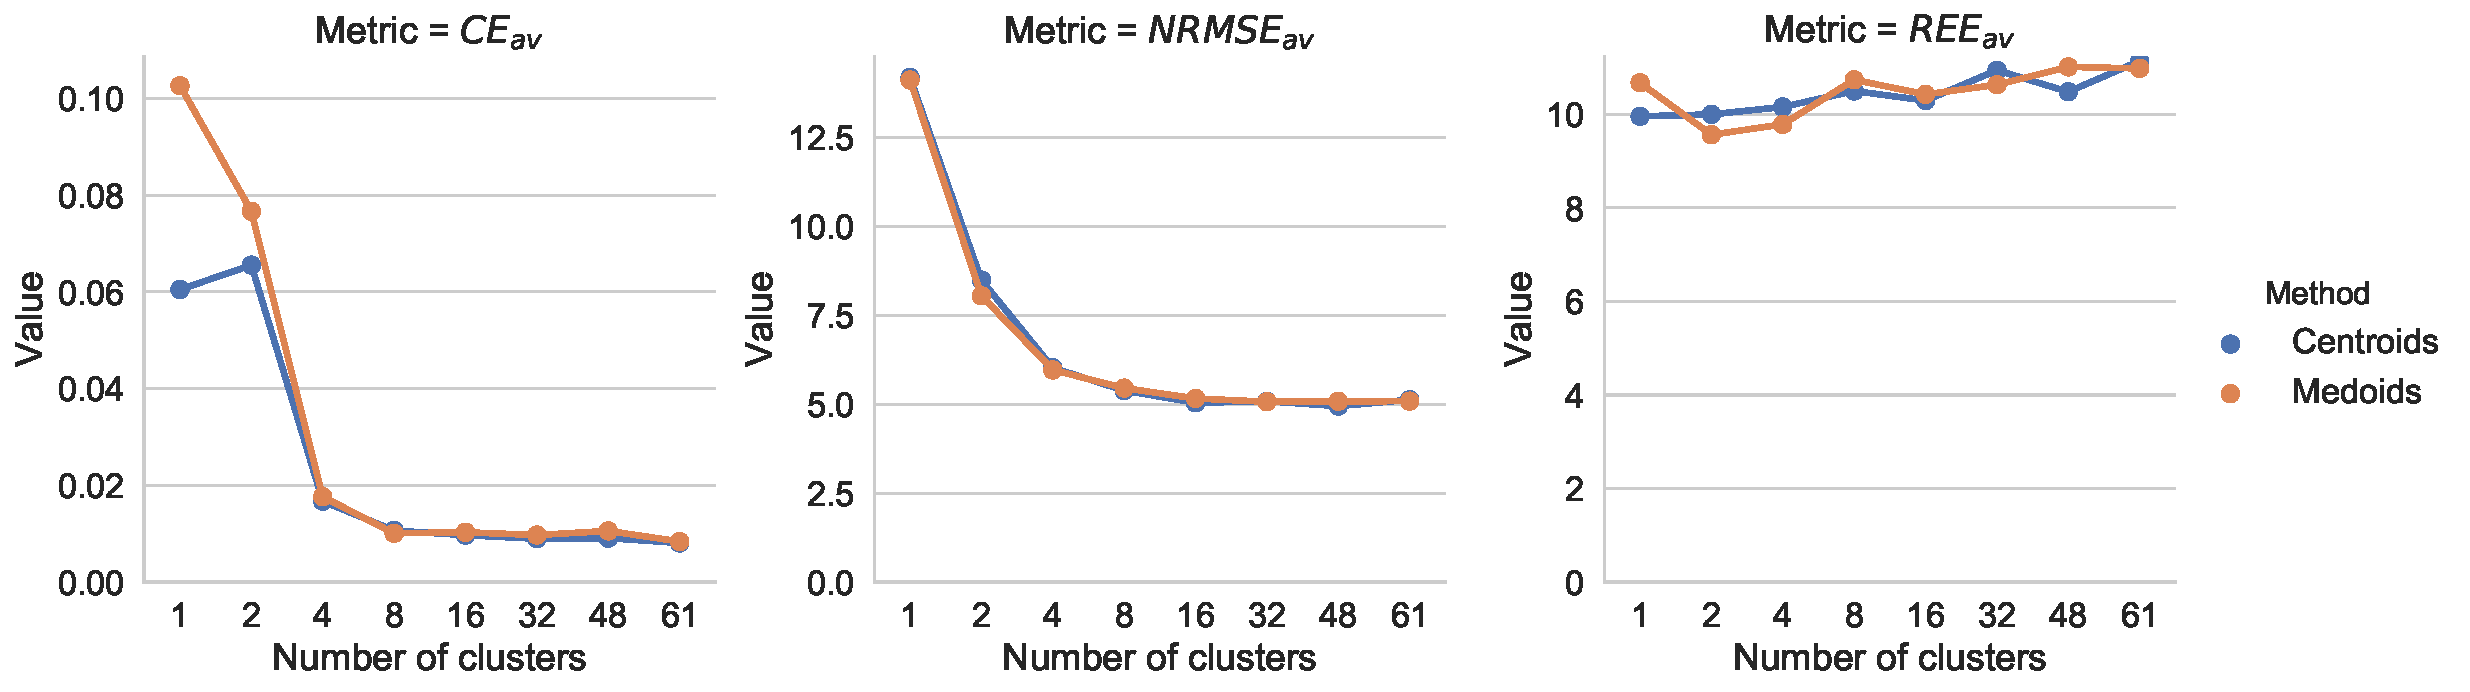
\includegraphics[width=\textwidth]{figures/methods_and_materials/clusters_compared.pdf}
%\caption{Comparison of number of clusters for accuracy.}
%\label{fig:clusters_compared}
%\end{figure*}
%
%The error metrics do not exhibit a significant difference between using either the centroids or medoids technique. However, we chose to use the medoids technique. This was done due to the fact that the extreme high and low values would not be lost due to averaging \cite{Hilbers2019}.
%
%Figure \ref{fig:clusters_compared_load} and Figure \ref{fig:clusters_compared_resources} display the resultant representative days that were used to represent an entire year in the simulation. A positive correlation between onshore and offshore wind speed can be seen in Figure \ref{fig:clusters_compared_resources}, which one would expect for the relatively small geography of the United Kingdom. Between the hours of 96 and 120 a negative correlation of solar irradiance and wind speed is exhibited, which may refer to a particularly sunny and windless day. Whereas between 72 and 96 a particularly windy and sunless day is exhibited.
%
%\begin{figure}
%\centering
%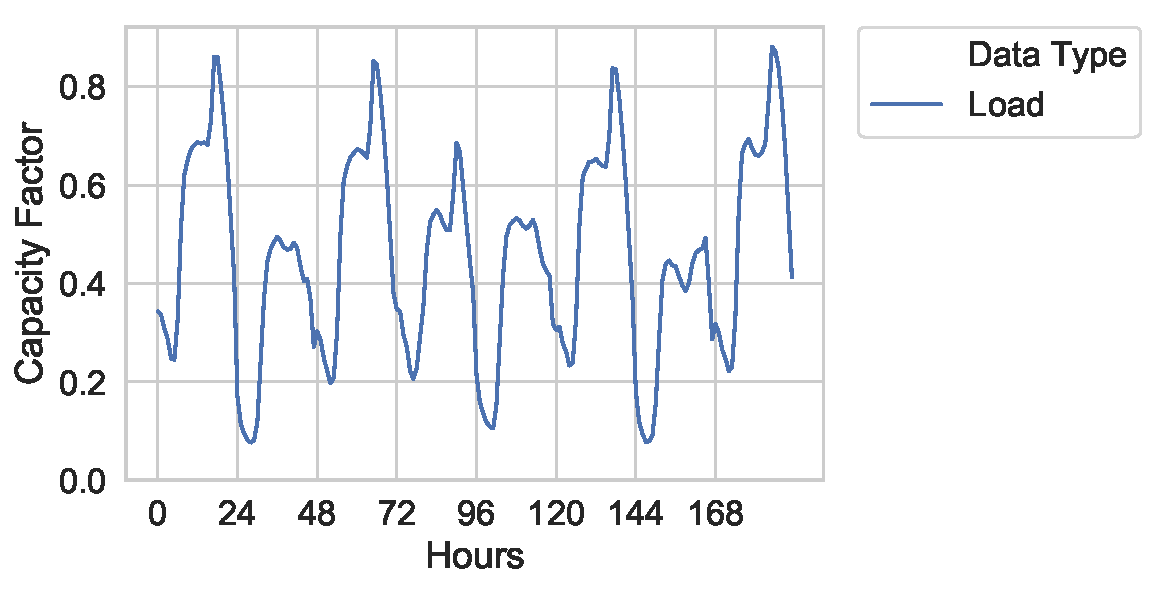
\includegraphics[width=0.49\textwidth]{figures/methods_and_materials/clusters_results_load.pdf}
%\caption{Representative days of electricity demand.}
%\label{fig:clusters_compared_load}
%\end{figure}
%
%Figure \ref{fig:clusters_compared_load} refers to the electrical load of the representative days. It should be noted that these representative days represent a quasi-temporal year and do not represent actual months.
%
%
%\begin{figure}
%\centering
%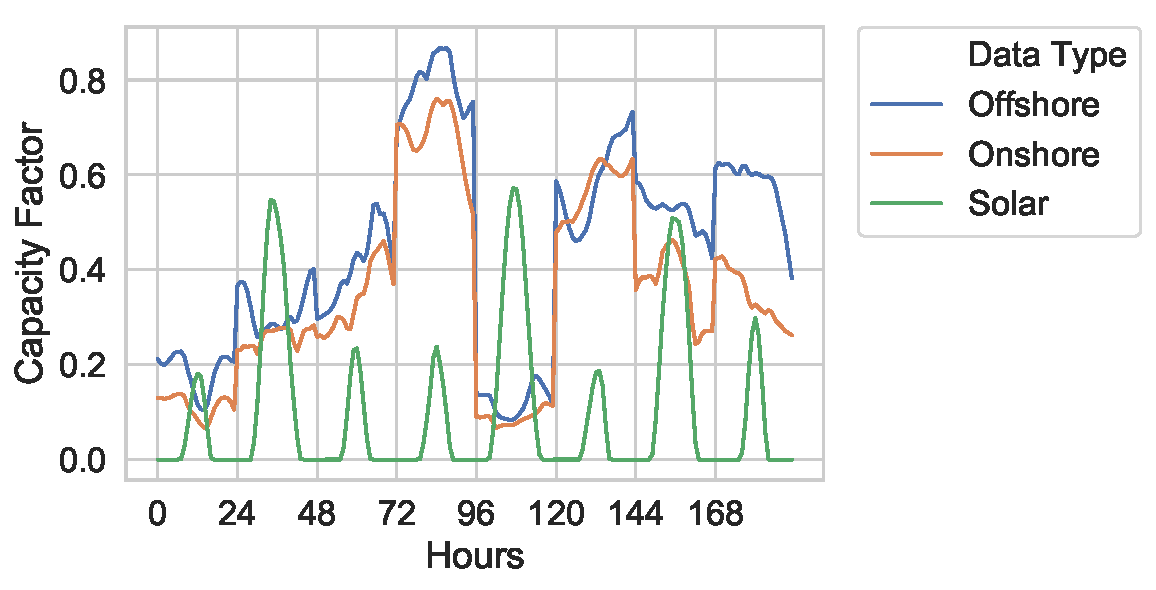
\includegraphics[width=0.49\textwidth]{figures/methods_and_materials/clusters_results_resources.pdf}
%\caption{Representative days of renewable resources.}
%\label{fig:clusters_compared_resources}
%\end{figure}


\subsubsection{Integrating higher temporal granularity}

To integrate the additional temporal granularity of the model, extra time-steps were taken per year. The higher temporal granularity of the model enabled us to accurately model the hourly fluctuations in solar and wind  which leads to more accurate expectations of the investment opportunities of these technologies ~\cite{Ludig2011,Haydt2011}.

GenCos make bids at the beginning of every time-step and the Power Exchange matches demand with supply in merit-order dispatch using a uniform pricing market. An example of electricity mix in a single representative day is shown in Figure \ref{fig:single_dispatched_day}. 

%
%\begin{equation}
%\label{eq:merit-order-dispatch}
%	\min_{b}
%	\sum\limits_{n=0}^{||b||}
%	\left(
%	b
%	\right)
%\end{equation}

Figure \ref{fig:single_dispatched_day} displays the high utilization of low marginal-cost generators such as nuclear, wind and photovoltaics. At hour 19, an increase in offshore wind leads to a direct decrease in CCGT. In contrast to this, a decrease in offshore and onshore between the hours of 8 and 12 lead to an increase in dispatch of coal and CCGT. One would expect this behaviour to prevent blackouts and meet demand at all times. This process has enabled us to more closely match fluctuations in IRES.

\begin{figure}
	\centering
	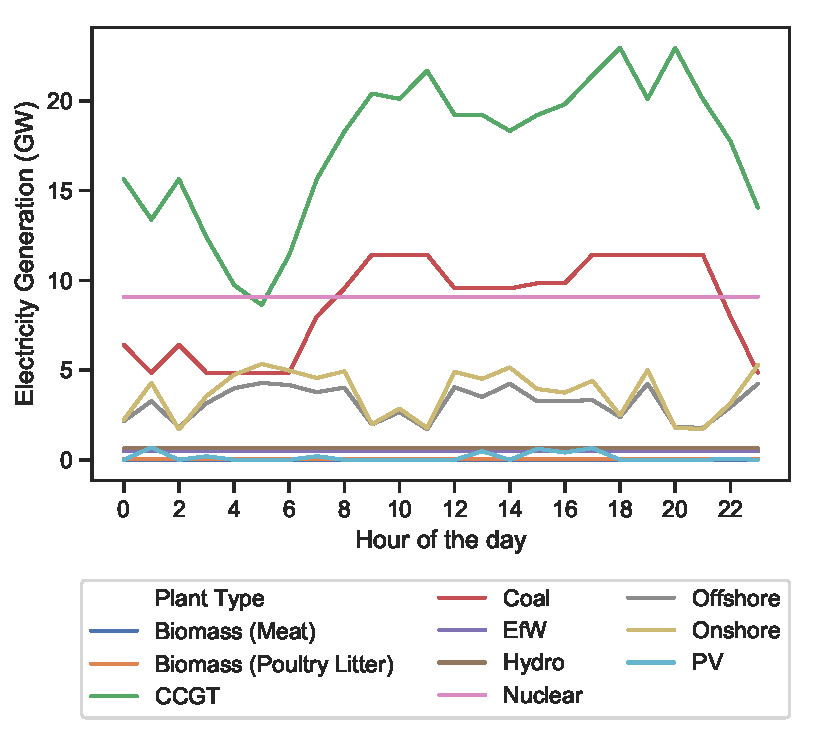
\includegraphics[width=0.7\textwidth]{Chapter4/figures/e-Energy-2020/methods_and_materials/clusters_results_single_day.pdf}
	\caption{Example of a single day of dispatched supply.}
	\label{fig:single_dispatched_day}
\end{figure}


\subsubsection{Evaluation of representative days}
\label{ssec:res_repr_days}

Figure \ref{fig:error_metrics_vs_cluster_number} displays the error metrics versus number of clusters. Both $CE_{av}$ and $NRMSE_{av}$ display similar behaviour for the $k$-means approach (centroids and medoids), namely the error improves significantly from a single cluster to eight clusters for both centroids and medoids. For the number of clusters greater than eight there are diminishing returns. For $REE_{av}$, however, the error metric is best at a single cluster, and gets worse with the number of clusters. The Wards approach, however, performs significantly worse for all metrics at every number of clusters. 



We chose eight clusters, for centroids and medoids, as a compromise between accuracy of the three error metrics and compute time of the simulation. This is because, eight was the largest number of clusters that gave us the lowest score for $CE_{av}$, $NRMSE_{av}$ and $REE_{av}$ without significantly increasing compute time. Whilst there was little significant difference between centroid and medoid, we chose to use the medoids due to the fact that the extreme high and low values would not be lost due to averaging \cite{Hilbers2019}.



%\begin{figure}
%	\centering
%	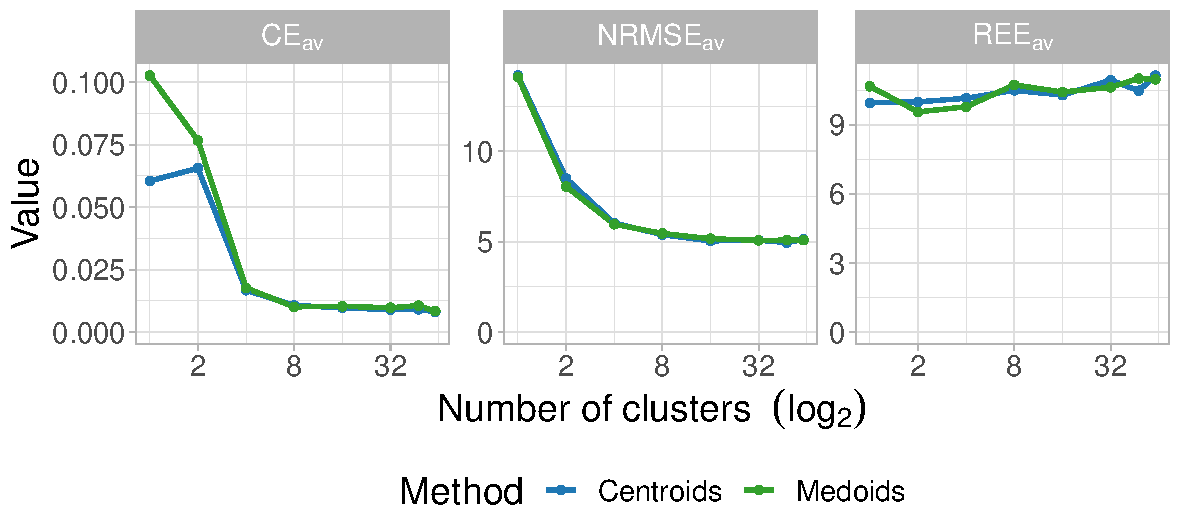
\includegraphics[width=0.8\textwidth]{Chapter4/figures/e-Energy-2020/methods_and_materials/clusters_compared_ggplot.pdf}
%	\caption{Number of clusters compared to error metrics.}
%	\label{fig:error_metrics_vs_cluster_number}
%\end{figure}


\begin{figure}
	\centering
	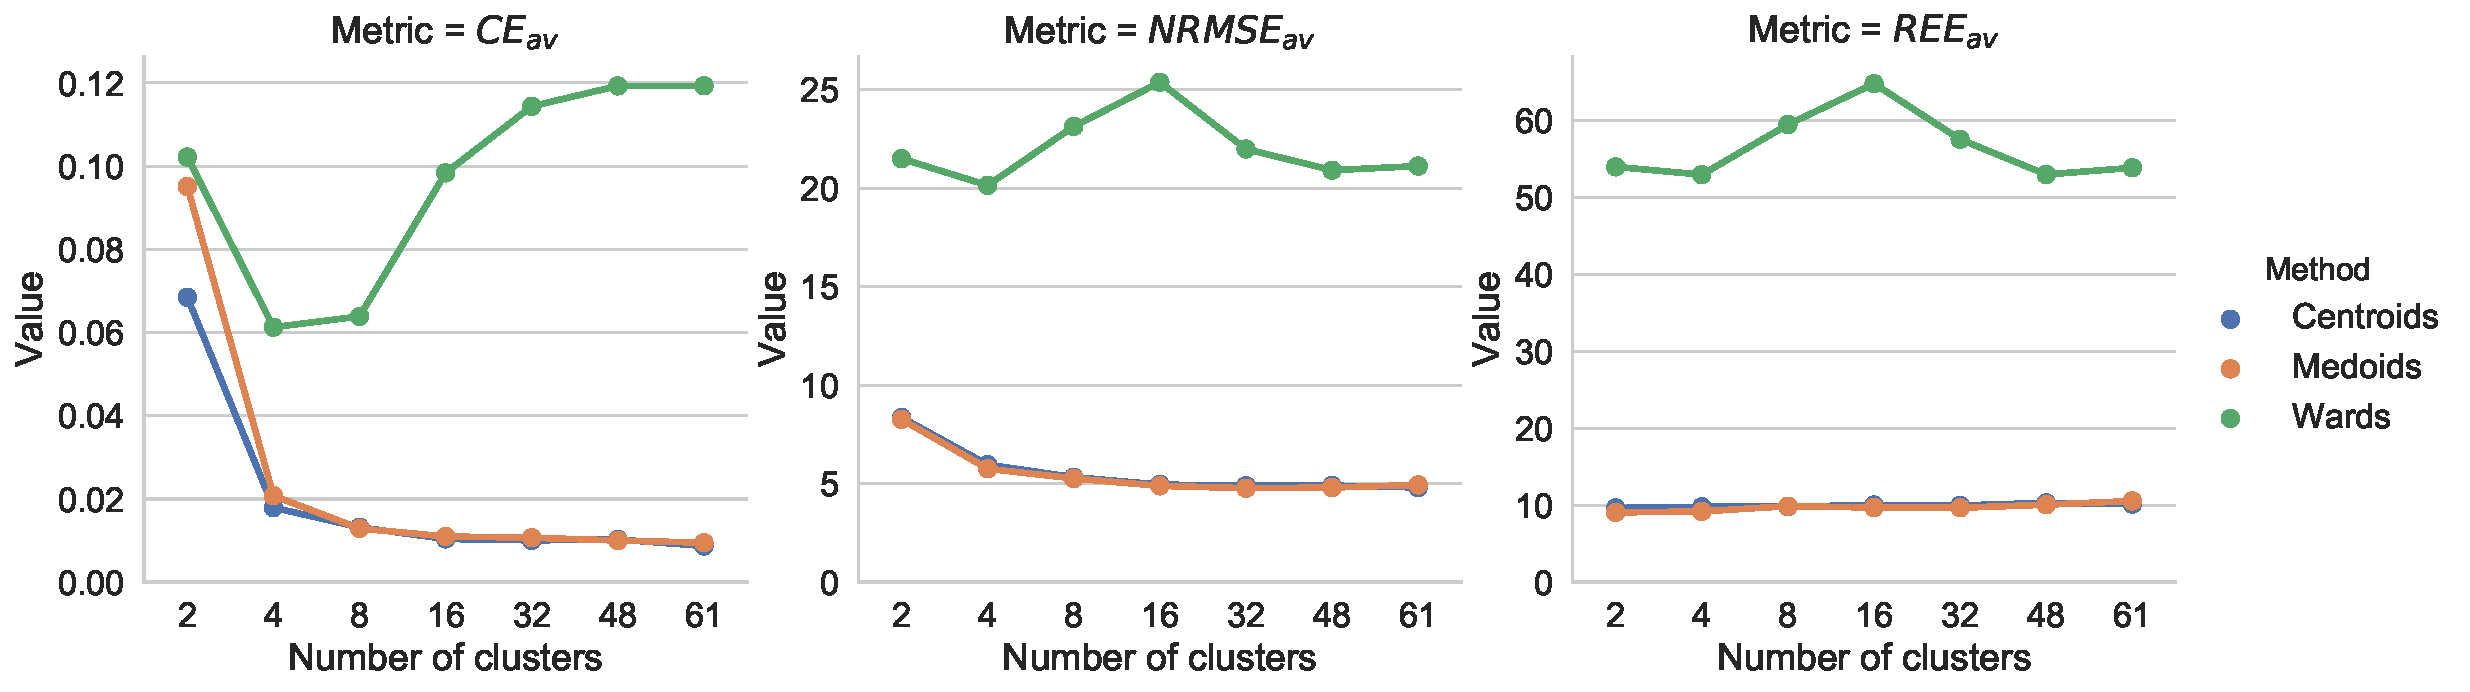
\includegraphics[width=0.9\textwidth]{Chapter4/figures/clusters_compared_wards.pdf}
	\caption{Number of clusters compared to error metrics.}
	\label{fig:error_metrics_vs_cluster_number}
\end{figure}





\section{Validation and performance}
\label{elecsim:sec:validation}

In this section we detail the validation approaches taken in our model. For this, we take two approaches. One is to compare the price duration curve of the actual vs. our simulated price duration curve in 2018 using the 20 time-steps per year approach. The other is to use cross-validation between the years 2013 and 2018, using our representative days approach.


\subsection{Price Duration Curve Validation}

Validation of models is important to ascertain that the output is accurate. However, it should be noted that these long-term simulations are not predictions of the future, rather possible outcomes based upon certain assumptions. Jager posits that a certain outcome or development path, captured by empirical data, might have developed in a completely different direction due to chance. However, the processes that emerge from a model should be realistic and in keeping with expected behaviour \cite{Jager2006a}.

We begin by comparing the price duration curve in the year 2018. Figure \ref{fig:price_duration_curve} shows the N2EX Day Ahead Auction Prices of the UK \cite{nordpool_2019}, the Monte-Carlo simulated electricity prices, and the non Monte-Carlo electricity price throughout the year 2018. Fuel prices varying throughout a year, as does $V_C$ and WACC. WACC is sampled from a Gaussian distribution with a standard deviation of $\pm3$\%. $V_C$ is sampled from a uniform distribution between 30\% and 200\% of the mean $V_C$ price, whilst fuel price is sampled from the residuals of an ARIMA model fit on historical data. The N2EX Day Ahead Market is a day ahead market run by Nord Pool AS. Nord Pool AS runs the largest market for electrical energy in Europe, measured in volume traded and in market share \cite{nordpool_2019}.



\begin{figure}
	\begin{center}
		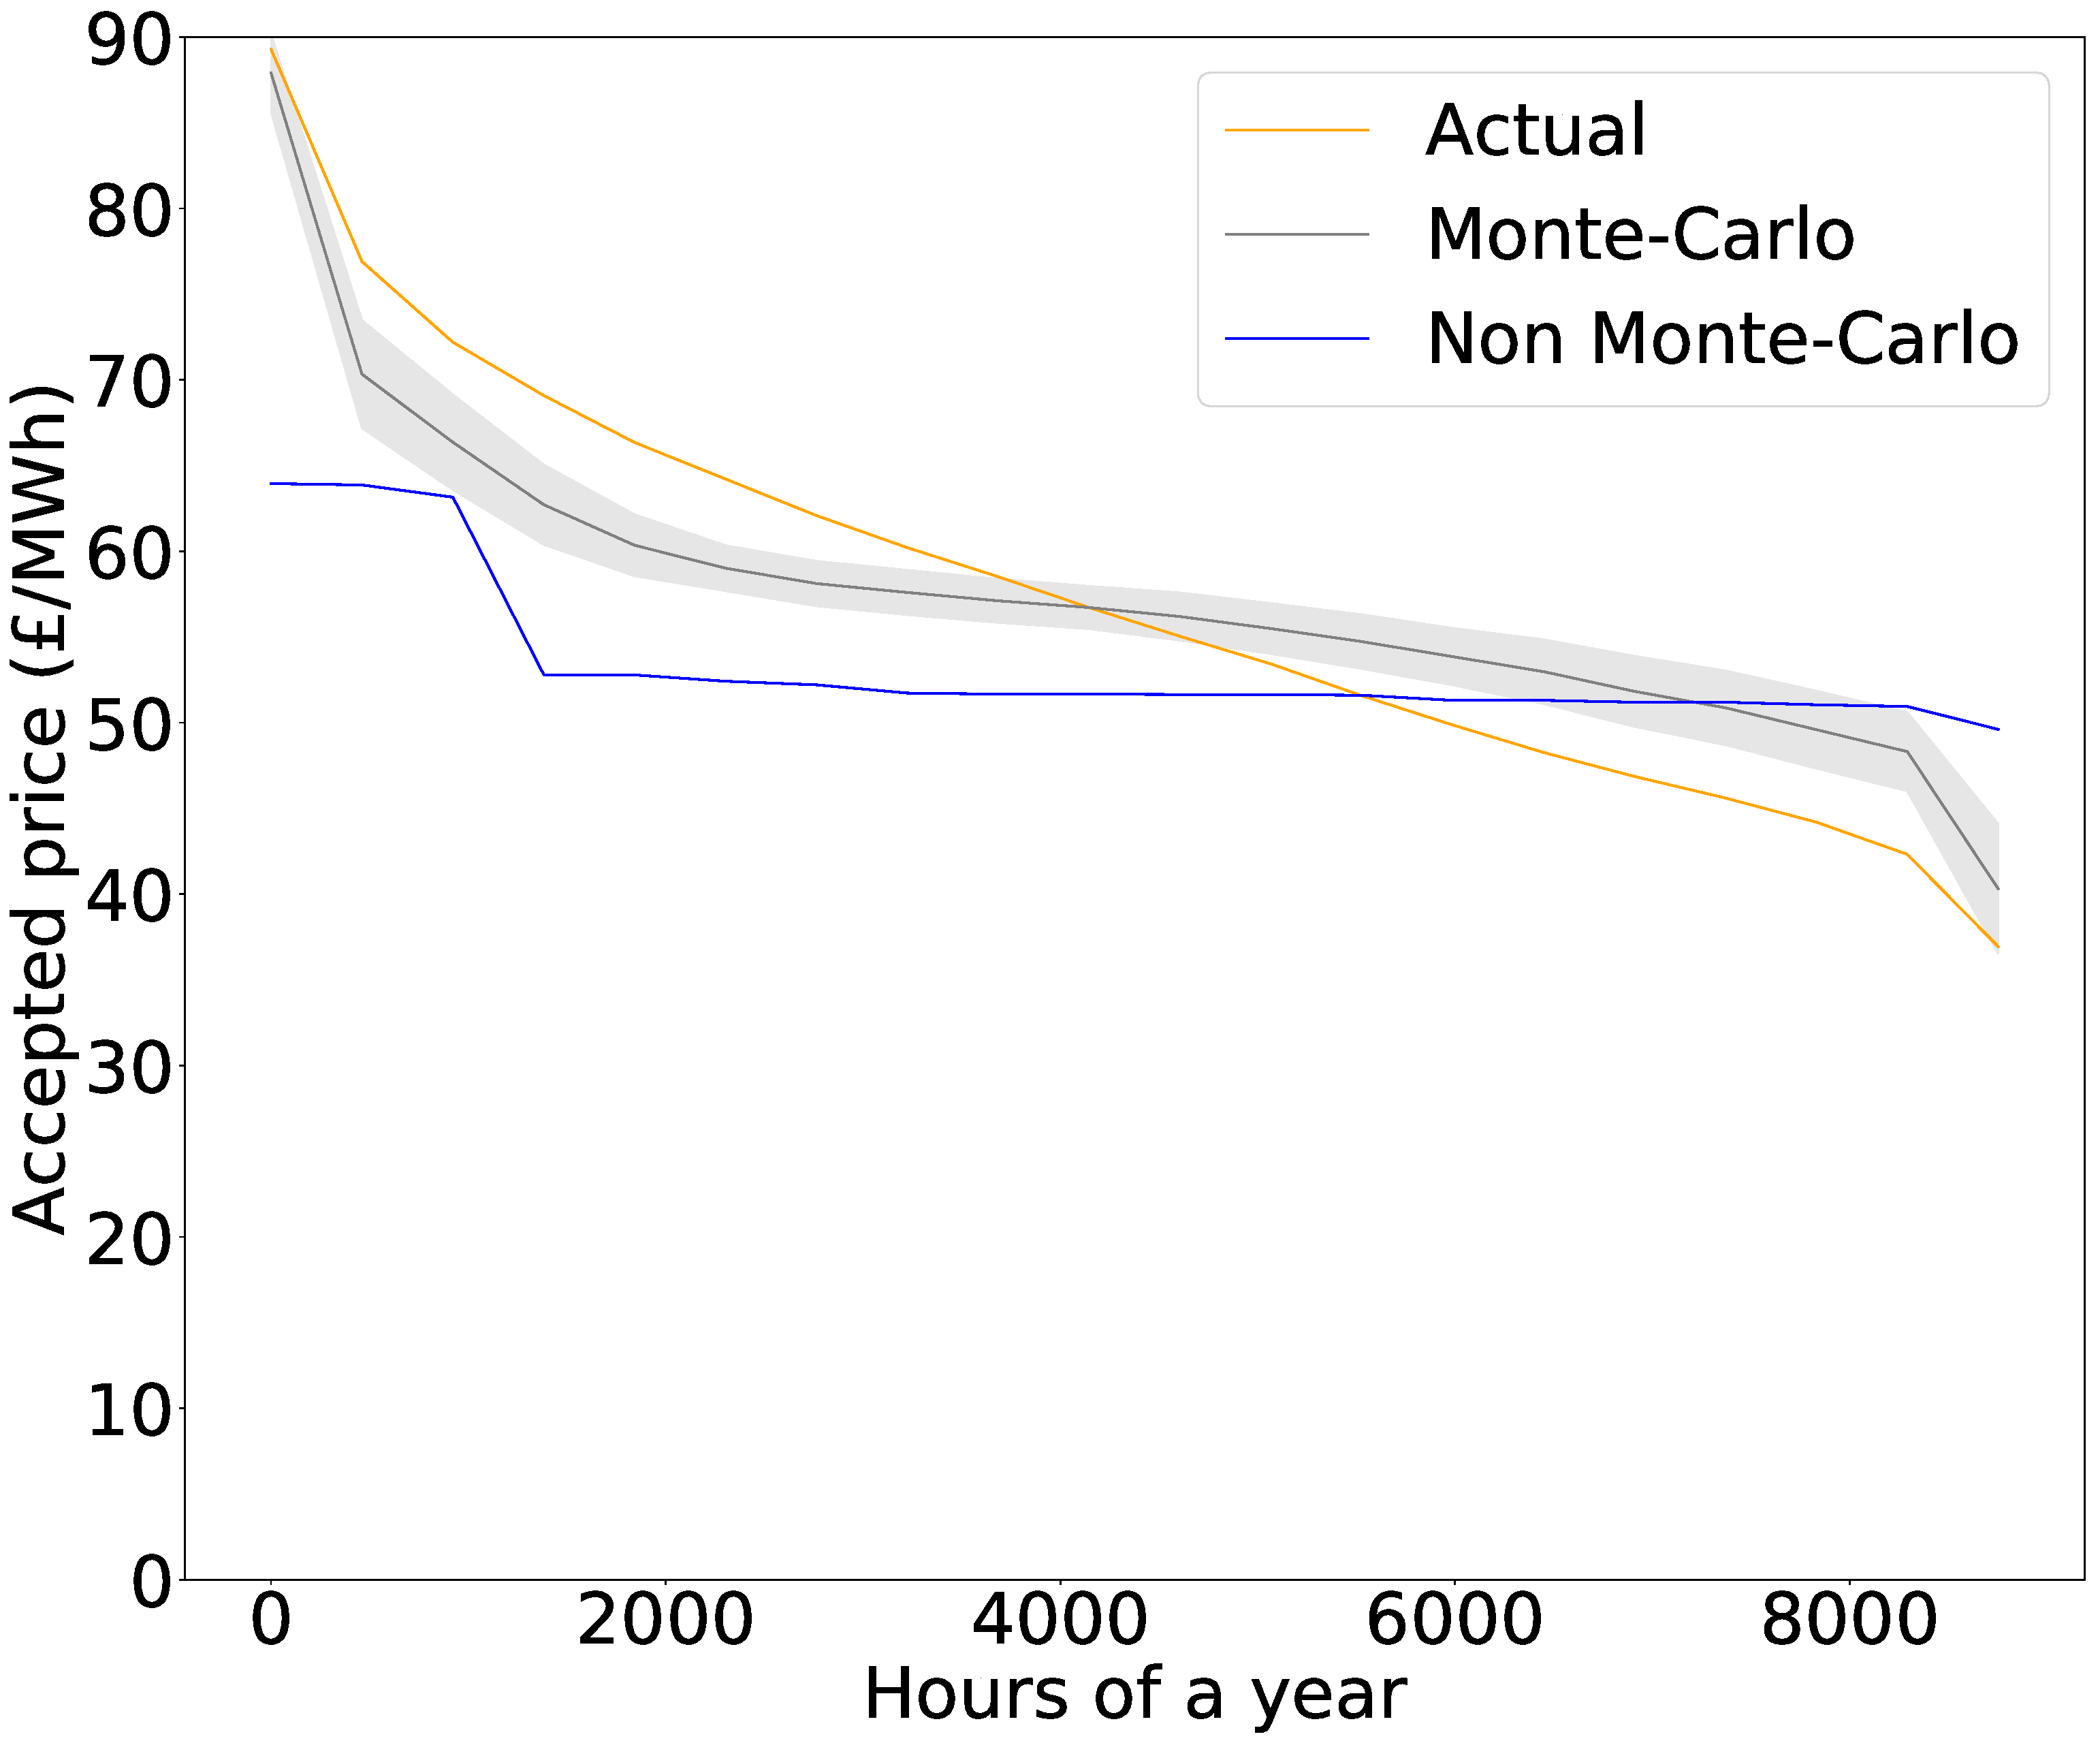
\includegraphics[width=0.6\textwidth]{Chapter4/figures/load_price_duration_curve_comparison-monte-carlo.pdf}
		\caption{Price duration curve which compares real electricity prices to those paid in ElecSim (2018).}
		\label{fig:price_duration_curve}
	\end{center}
\end{figure}

%\begin{table}
%	\centering
%	\csvautobooktabular{tables/validation/initialisation_run_validation.csv}
%	\caption{Validation performance metrics.}
%	\label{table:validation_metrics}
%\end{table}





We ran the initialisation of the model 40 times to capture the price variance. Outliers were removed as on a small number of occasions large jumps in prices at peak demand occurred which deviated from the mean. We did this, as although this does occur in real life, it occurs at a smaller fraction of the time than 5\% of the year (twenty time-steps per year), therefore the results would be unreasonably skewed for the highest demand segment. 

Figure \ref{fig:price_duration_curve} demonstrates very little variance in the non-stochastic case. This is due to the fact that combined cycle gas turbines (CCGTs) set the spot price. These CCGTs have little variance between one another as they were calibrated using the same dataset. By adding stochasticity of fuel prices and operation and maintenance prices, a curve that more closely resembles the actual data occurs. The stochastic curve, however, does not perfectly fit the real data, which may be due to higher variance in fuel prices and historical differences in operation and maintenance costs between power plants. One method of improving this would be fitting the data used to parametrise to the curve.

Table \ref{table:validation_metrics} shows performance metrics of the stochastic and non-stochastic runs versus the actual price duration curve . The stochastic implementation, improves the mean absolute error (MAE) of the non-stochastic case by $52.5\%$.

\begin{table}[]
	\begin{tabular}{p{4cm}p{4cm}p{2.5cm}p{3cm}}
		\hline
		Metric & N2EX Day Ahead & ElecSim & Non Monte-Carlo \\ \hline
		Avg. Price (\textsterling/MWh) & 57.49 & 57.52 & 53.39 \\
		Std. dev (\textsterling/MWh) & - & 9.64 & - \\
		MAE (\textsterling/MWh) & - & 3.97 & 8.35 \\
		RMSE (\textsterling/MWh) & - & 4.41 & 10.2 \\ \hline
	\end{tabular}
	\caption{Validation performance metrics.}
	\label{table:validation_metrics}
\end{table}

%By observing the processes that emerge from the long-term scenarios, we can see that carbon price and investment in renewable generation are positively correlated, as would be expected. The highest NPV calculations were for onshore wind and CCGT plants. This is realistic for the United Kingdom, where subsidies are required for other forms of generation such as coal and nuclear.



%%%%%%%%%%%%%%%%%%%%%%%%%%%%%%%%%%%%%%%%%%%%%%%%
%%%%%%%%%%%%%%%%%%%%%%%%      Paper 2    %%%%%%%%%%%%%%%%
%%%%%%%%%%%%%%%%%%%%%%%%%%%%%%%%%%%%%%%%%%%%%%%%


\subsection{Representative days validation}
\label{elecsim:ssec:representative_validation}

In this section we detail the approach taken in this paper to validate our model using representative days as time-steps. 

To achieve this, we use a genetic algorithm to find the predicted price duration curves which lead to the smallest error between our simulated electricity mix and the scenarios tested. The scenarios examined here are the observed electricity mix of the UK between 2013 and 2018 and the BEIS reference scenario projected in 2018 till 2035. When projecting the BEIS reference scenario we also optimise for nuclear subsidy and uncertainty in the price duration curves.


%For GenCos to adequately make investments, they must formulate an expectation of future electricity prices over the lifetime of a plant. For this paper, we use the net present value (NPV) metric to compare investments. 


%NPV provides a method for evaluating and comparing investments with cash flows spread over many years, making it suited for evaluating power plants which have a long lifetime.  

%Equation \ref{eq:npv_eq} is the calculation of NPV, where $t$ is the year of the cash flow, $i$ is the discount rate, $N$ is the total number of years, or lifetime of power plant, and $R_t$ is the net cash flow of the year $t$.
%\begin{equation} \label{eq:npv_eq}
%NPV(i, N) = \sum_{t=0}^{N}\frac{R_t}{(1+t)^t}
%\end{equation}

As mentioned in Section \ref{elecsim:sec:architecture}, GenCos make investments based upon the net present value. As shown in Equation \ref{architecture:eq:npv_eq}, an expectation of the net cash flow, $R_t$ is required. 

The net cash flow, $R_t$, is calculated by subtracting both the operational and capital costs from revenue over the expected lifetime of the prospective plant. The revenue gained by each prospective plant is the expected price they will gain per expected quantity of MWh sold over the expected lifetime of the plant. This is shown formally in Equation \ref{eq:revenue_total}:


\begin{equation}
\label{eq:revenue_total}
R_t = 
\sum\limits_{t=0}^T 
\sum\limits_{h=0}^H
\sum\limits_{m=0}^M \left(
m_{h,t}(PPDC_{h,t}
-
C_{var_{h,t}})\right)
- C_c
\end{equation}

\noindent where $m_{h,t}$ is the expected quantity of megawatts sold in hour $h$ of year $t$. $PPDC_{h,t}$ is the predicted price duration curve at year $t$ and hour $h$. $C_{var_{h,t}}$ is the variable cost of the power plant, which is dependent on expected megawatts of electricity produced, $C_c$ is the capital cost.

The predicted price duration curve ($PPDC_{h,t}$) is an expectation of future electricity prices over the lifetime of the plant. The $PPDC_{h,t}$ is a function of supply and demand. However, with renewable electricity generator costs falling, future prices are uncertain and largely dependent upon long-term scenarios of electricity generator costs, fuel prices, carbon taxes and investment decisions. \cite{IRENA2014}. Due to the uncertainty of future electricity prices over the horizon of the lifetime of a power plant we have set future electricity prices as an exogenous variable that can be set by the user in ElecSim. 


To gain an understanding of expected electricity prices that lead to particular scenarios we use a genetic algorithm optimisation approach. This enables us to understand the range of future electricity prices that lead to certain scenarios developing. In addition, it allows us to understand whether the parameters required for certain scenarios to develop are realistic. This enables us to check the assumptions of our model and the likelihood of scenarios. Further, using these optimised parameters, we are better able to further explore `\textit{what-if}' scenarios.















To verify the accuracy of the underlying dynamics of ElecSim, the model was initialised to data available in 2013 and allowed to develop until 2018. We used a genetic algorithm to find the optimum price duration curve predicted ($PPDC$) by the GenCos 10 years ahead of the year of the simulation. This $PPDC$ was used to model expected rate of return of prospective generation types, as shown in Equations \ref{eq:npv_eq} and \ref{eq:revenue_total}. 

The genetic algorithm's objective was to reduce the error of simulated and observed electricity mix in the year 2018 by finding a suitable $PPDC$ used by each of the GenCos for investment evaluation.

\subsubsection{Scenario}

For this experiment, we initialised ElecSim with parameters known in 2013 for the UK. ElecSim was initialised with every power plant and respective GenCo that was in operation in 2013 using the BEIS DUKES datatset \cite{dukes_511}. The funds available to each of the GenCos was taken from publicly released official company accounts at the end of 2012 \cite{companies_house}.

To ensure that the development of the electricity market from 2013 to 2018 was representative of the actual scenario between these years, we set the exogenous variables, such as carbon and fuel prices, to those that were observed during this time period. In other words, the scenario modelled equated to the observed scenario. 

The data for the observed EU Emission Trading Scheme (ETS) price between 2013 and 2018 was taken from \cite{eu-ets}. Fuel prices for each of the fuels were taken from \cite{beis_fuel_price}. The electricity load data was modelled using data from \cite{gbnationalgridstatus_2019}, offshore and onshore wind and solar irradiance data was taken from \cite{Pfenninger2016}. There were three known significant coal plant retirements in 2016. These were removed from the simulation at the beginning of 2016.



\subsubsection{Optimisation problem}
\label{ssec:optimisation-problem}

The price duration curve was modelled linearly in the form $y=mx+c$, where $y$ is the cost of electricity, $m$ is the gradient, $x$ is the demand of the price duration curve and $c$ is the intercept.

Equation \ref{eq:problem_formulation} details the optimisation problem formally:

\begin{equation}
\label{eq:problem_formulation}
\min_{m,c} \sum\limits_{o\in O}\left(
\frac{\left|A_o-f_o(m,c)\right|}
{\left|\left|O\right|\right|}
\right)
\end{equation}

\noindent where $o\in O$ refers to the average percentage electricity mix during 2018 for wind (both offshore and onshore generation), nuclear, solar, CCGT, and coal, where $O$ refers to the set of these values. $A_o$ refers to observed electricity mix percentage for the respective generation type in 2018. $f_o(m,c)$ refers to the simulated electricity mix percentage for the respective generation type, also in 2018. The input parameters to the simulation are $m$ and $c$ from the linear $PPDC$, previously discussed, ie. $y=mx+c$. $\left|\left|O\right|\right|$ refers to the cardinality of the set.



\subsection{Long-Term Scenario Analysis}
\label{sssec:scen-analysis}

In addition to verifying the ability for ElecSim to mimic observed investment behaviour over 5 years, we compared ElecSim's long-term behaviour to that of the UK Government's Department for Business, Energy and Industrial Strategy (BEIS) \cite{DBEIS2019}. This scenario shows the projections of generation by technology for all power producers from 2018 to 2035 for the BEIS reference scenario. This is the same scenario as discussed in the next section.

\subsubsection{Scenario}
\label{sssec:scenario-details}

We initialised the model to 2018 based on \cite{Kell}. The scenario for development of fuel prices and carbon prices were matched to that of the BEIS reference scenario \cite{DBEIS2019}.


\subsubsection{Optimisation problem} The optimisation approach taken was a similar process to that discussed in Sub-Section \ref{ssec:optimisation-problem}, namely using a genetic algorithm to find the optimum expected price duration curve. However, instead of using a single expected price duration curve for each of the agents for the entire simulation, we used a different expected price duration curve for each year, leading to 17 different curves. This enabled us to model the non-static dynamics of the electricity market over this extended time period. 

In addition to optimising for multiple expected price duration curves, we optimised for a nuclear subsidy, $S_n$. Further, we optimised for the uncertainty in the expected price parameters $m$ and $c$, named $\sigma_m$ and $\sigma_c$ respectively, where $\sigma$ is the standard deviation in a normal distribution. $m$ and $c$ are the parameters for the predicted price duration curve, as previously defined, of the form $y=mx+c$.  

This enabled us to model the different expectations of future price curves between the independent GenCos. The addition of a nuclear subsidy as a parameter is due to the likely requirement for Government to provide subsidies for new nuclear \cite{Suna2016}.

A modification was made to the reward algorithm for the long-term scenario case. Rather than using the discrepancy between observed and simulated electricity mix in the final year (2018) as the reward, a summation of the error metric for each simulated year was used. This is detailed formally in Equation \ref{eq:long-term-reward}:


\begin{equation}
\label{eq:long-term-reward}
\min_{m\in M,m\in C} 
\sum\limits_{y\in Y}
\sum\limits_{o\in O}\left(
\frac{\left|A_{y_o}-f_{y_o}(m_y,c_y)\right|}
{\left|\left|O\right|\right|}
\right)
\end{equation}

\noindent where $M$ and $C$ are the sets of the 17 parameters of $m_y$ and $c_y$ respectively for each year, $y$. $y\in Y$ refers to each year between 2018 and 2035. $m_y$ and $c_y$ refer to the parameters for the predicted price duration curve, of the form $y=mx+c$ for the year $y$. $A_{y_o}$ refers to the actual electricity mix percentage for the year $y$ and generation type $o$. Finally, $f_{y_o}(m_y,c_y)$ refers to the simulated electricity mix percentage with the input parameters to the simulation of $m$ and $c$ for the year $y$.












\subsection{Genetic Algorithms}
\label{elecsim:ssec:geneticalgorithm}

Genetic Algorithms (GAs) are a type of evolutionary algorithm which can be used for optimisation. We chose the genetic algorithm for this application due to its ability to find good solutions with a limited number of simulation runs, ability for parallel computation and its ability to find global optima. These characteristics are useful for our application, as a single simulation can take up to 36 hours. 

In this section we detail the genetic algorithm used in this paper. Initially, a population $P_{0}$ is generated for generation 0. This population of individuals is used for the parameters to the simulation. The output of the simulations for each of the individuals are then evaluated. A subset of these individuals $C_{t+1} \subset P_{t}$ are chosen for mating. This subset is selected proportional to their fitness. With `fitter' individuals having a higher change of reproducing to create the offspring group $C'_{t+1}$. $C'_{t+1}$ have characteristics dependent on the genetic operators: crossover and mutation. The genetic operators are an implementation decision \cite{FogelDavidB2009}. 

Once the new population has been created, the new population $P_{t+1}$ is created by merging individuals from $C'_{t+1}$ and $P_{t}$. See Algorithm \ref{genetic-algorithm} for detailed pseudocode.

We used the DEAP evolutionary computation framework to create our genetic algorithm \cite{Gagn2012}. This framework gave us sufficient flexibility when designing our genetic algorithm. Specifically, it enabled us to persist the data of each generation after every iteration to allow us to verify and analyse our results in real-time.

%
\begin{algorithm}[t]
	\begin{algorithmic}[1]
		\State $t=0$
		\State initialize $P_{t}$
		\State evaluate structures in $P_{t}$
		\While {termination condition not satisfied}
		\State $t=t+1$
		\State select reproduction $C_{t}$ from $P_{t-1}$
		\State recombine and mutate structures in $C_{t}$
		
		forming $C'_{t}$
		\State evaluate structures in $C'_{t}$
		\State select each individual for $P_{t}$ from $C'_{t}$ 
		
		or $P_{t-1}$
		\EndWhile
		\caption{Genetic algorithm \cite{FogelDavidB2009}}
		\label{genetic-algorithm}
	\end{algorithmic}
\end{algorithm}

\subsubsection{Parameters for Validation with Observed Data}
\label{ssec:ga_params_valid}

The parameters chosen for the problem explained in Section \ref{sssec:scen-analysis} was a population size of $120$, a crossover probability of $50\%$, a mutation probability of $20\%$ and the parameters, $m$ and $c$, as per Equation \ref{eq:problem_formulation}, were given the bounds of $[0.0, 0.004]$ and $[-30, 100]$ respectively. 

The bounds for $m$ and $c$ were calculated to ensure a positive price duration curve, with a maximum price of \textsterling300 for $50,000$MW. The population size was chosen to ensure a wide range of solutions could be explored, whilst limiting compute time to ${\sim}$1 day per generation to allow for sufficient verification of the results. The crossover and mutation probabilities were chosen due to suggestions from the DEAP evolutionary computation framework \cite{Gagn2012}.


\subsubsection{Parameters for Long-Term Scenario Analysis}

The parameters chosen for the genetic algorithm for the problem discussed in Section \ref{sssec:scen-analysis} are displayed here. The population size was $127$, a crossover probability of $50\%$, a mutation probability of $20\%$. The parameters $m_y$, $c_y$ were given the bounds $[0.0, 0.003]$ and $[-30, 50]$ respectively, whilst $\sigma_m$ and $\sigma_c$ were both given the bounds of $[0, 0.001]$.

The population size was slightly increased, and the bounds reduced when compared to the parameters for Section \ref{ssec:ga_params_valid}. This was to increase the likelihood of convergence to a global optima, which was more challenging to achieve due to the significantly higher number of parameters.


\subsection{Results}
\label{sec:results}

Here we present the results of the problem formulation of Section \ref{sssec:scen-analysis}. Specifically, we compare the ability of our model to that of BEIS in the context of a historical validation between 2013 and 2018 of the UK electricity market. We also compare our ability to generate scenarios up to 2035 with that of BEIS. 

\subsubsection{Validation with Observed Data}

Figure \ref{elecsim:fig:beis_elecsim_historic_comparison} displays the output of ElecSim under the validation scenario, BEIS' projections and the observed electricity mix between 2013 and 2018, as explained in Section \ref{elecsim:ssec:representative_validation}.

\begin{figure}
	\centering
	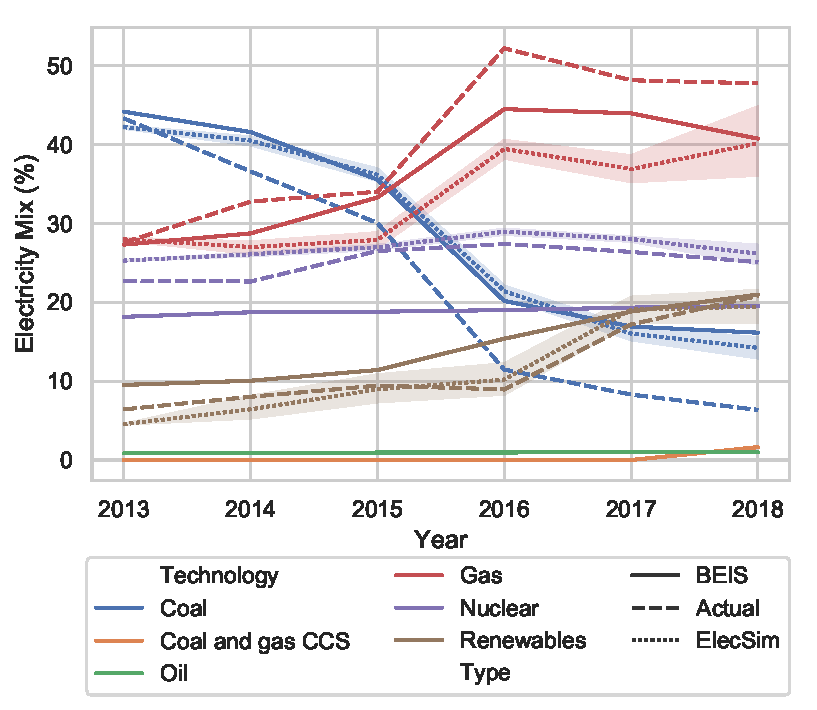
\includegraphics[width=0.7\columnwidth]{Chapter4/figures/e-Energy-2020/results/throughout_years_beis_elecsim_comparison_coal_dropout_leg_below.pdf}
	\caption{Comparison of actual electricity mix vs. ElecSim vs. BEIS projections and taking three coal power plants out of service.}
	\label{elecsim:fig:beis_elecsim_historic_comparison}
\end{figure}

The observed electricity mix changed significantly between 2013 and 2018. A continuous decrease of electricity production from coal throughout this period was observed. 2015 and 2016 saw a marked decrease of coal, which can be explained by the retirement of 3 major coal power plants. The decrease in coal between 2013 and 2016 was largely replaced by an increase in gas. After 2016, renewables play an increasingly large role in the electricity mix and displace gas.

Both ElecSim and BEIS were able to model the fundamental dynamics of this shift from coal to gas as well as the increase in renewables. Both models, however, underestimated the magnitude of the shift from coal to gas. This could be due to unmodelled behaviours such as consumer sentiment towards highly polluting coal plants, a prediction from industry that gas would become more economically attractive in the future or a reaction to The Energy Act 2013 which aimed to close a number of coal power stations over the following two decades \cite{uk_energy_act}.

%Both ElecSim and BEIS performed similarly in projecting the uptake in renewables. Whilst both models were able to accurately project the final renewable electricity mix in 2018, the observed uptake in renewables began to increase in 2015, as opposed to 2016. This could be explained by the increased wind speeds and rainfall observed during 2015 \cite{pa_2013_renewables}.

ElecSim was able to closely model the increase in renewables throughout the period in question, specifically predicting a dramatic increase in 2017. This is in contrast to BEIS who predicted that an increase in renewable energy would begin in 2016. However, both models were able to accurately predict the proportion of renewables in 2018. 

ElecSim was able to better model the observed fluctuation in nuclear power in 2016. BEIS, on the other hand, projected a more consistent nuclear energy output. This small increase in nuclear power is likely due to the decrease in coal during that year. BEIS consistently underestimated the share of nuclear power. 


%ElecSim and BEIS performed similarly with respect to the uptake in renewable energy  


%\subsection{Validation results and comparison}


%Figure \ref{fig:actual_vs_simulated_validation} shows the simulated electricity mix compared to the actual electricity mix between the years of 2013 to 2018 for the best price duration parameter set.


%\begin{figure}
%\centering
%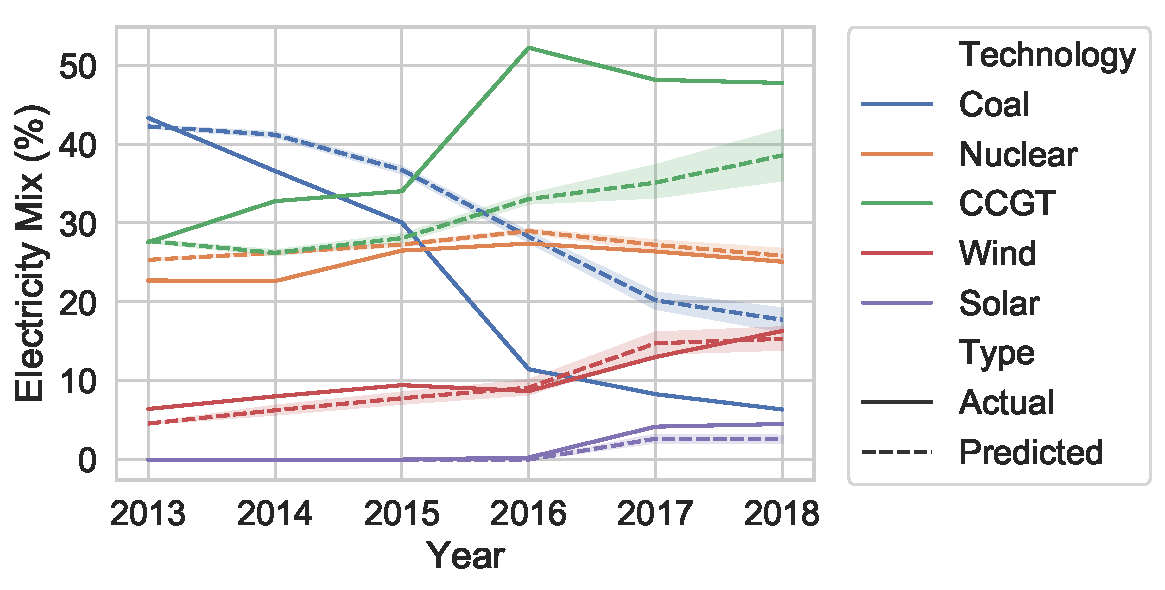
\includegraphics[width=0.49\textwidth]{figures/results/throughout_years.pdf}
%\caption{Electricity mix actual vs. simulated for validation scenario with eight representative days.}
%\label{fig:actual_vs_simulated_validation}
%\end{figure}

%


%Figure \ref{fig:actual_vs_simulated_validation} shows a rapid uptakes in solar and wind from the year of 2016, which closely matches the actual uptake. As well as this, the actual mix displays a rapid transition from coal to CCGT. Whilst ElecSim matches this trend, it is not matched precisely. 
%
%Figure \ref{fig:uk_validated_results_2018} compares the electricity mix in the year 2018 for actual and simulated by ElecSim for the optimal predicted price duration curve. 




%We compare our projections from 2013 to 2018 with the UK Governments (BEIS) projections made in 2013 in Figure \ref{fig:beis_elecsim_historic_comparison} \cite{UKDECC2013}. BEIS were also unable to precisley match the transition from coal to CCGT. However, they were able to model the large transition of coal to CCGT in the year 2016.
%
%However, the BEIS projection overestimates the uptake in renewables in the year 2016, which ElecSim does not.


%\begin{figure}
%\centering
%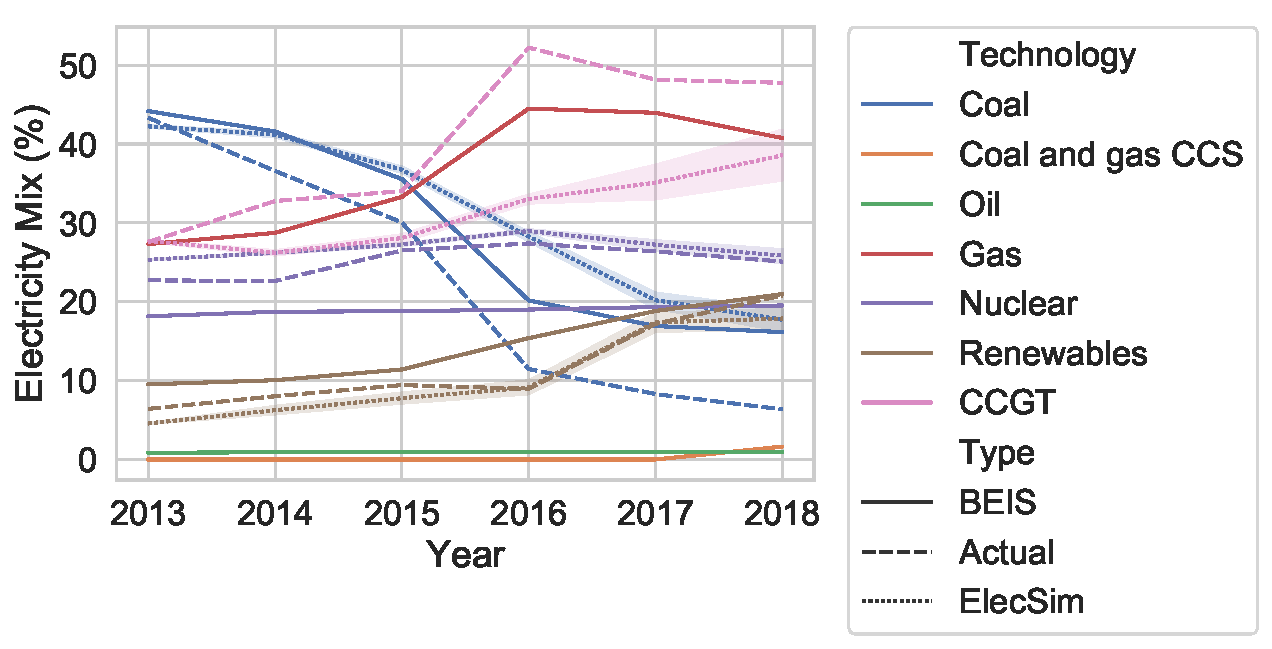
\includegraphics[width=0.49\textwidth]{figures/results/throughout_years_beis_elecsim_comparison.pdf}
%\caption{Comparison of actual electricity mix vs. ElecSim vs. BEIS projections.}
%\label{fig:beis_elecsim_historic_comparison}
%\end{figure}



%\begin{figure}
%\centering
%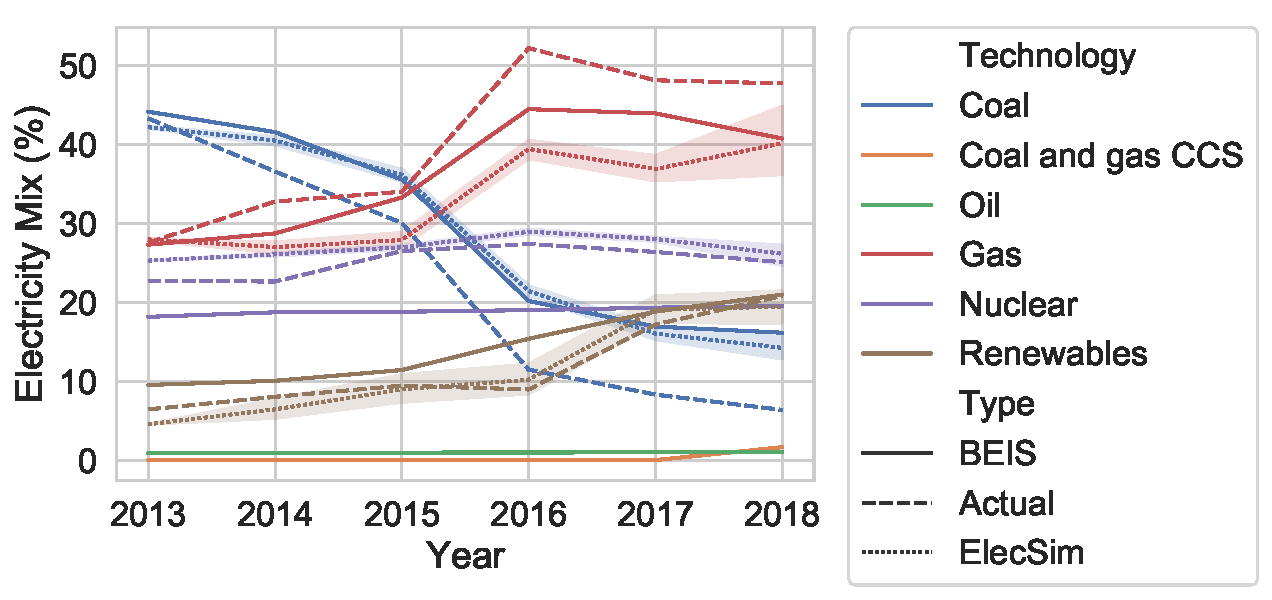
\includegraphics[width=0.49\textwidth]{figures/results/throughout_years_beis_elecsim_comparison_coal_dropout.pdf}
%\caption{Comparison of actual electricity mix vs. ElecSim vs. BEIS projections and taking three coal power plants out of service.}
%\label{fig:beis_elecsim_historic_comparison}
%\end{figure}






We display the error metrics to evaluate our models 5 year projections in Table \ref{table:metrics}. Where MAE is mean absolute squared error, MASE is mean absolute scaled error and RMSE is root mean squared error.

We are able to improve the projections for all generation types when compared to the naive forecasting approach using ElecSim, as shown by the MASE. Where the naive approach is simply predicting the next time-step by using the last known time-step. In this case the last known time-step is the electricity mix percentage for each generation type in 2013. 

\begin{table}[htb]
	\centering
	\csvautobooktabular{Chapter4/table_data/results/error_metrics.csv}
	\caption{Error metrics for time series forecast from 2013 to 2018.}
	\label{table:metrics}
\end{table}

Figure \ref{fig:best_price_curve} displays the optimal predicted price duration curve ($PPDC$) found by the genetic algorithm. This price curve was used by the GenCos to achieve the results shown in Figure \ref{fig:beis_elecsim_historic_comparison}. 


\begin{figure}
	\centering
	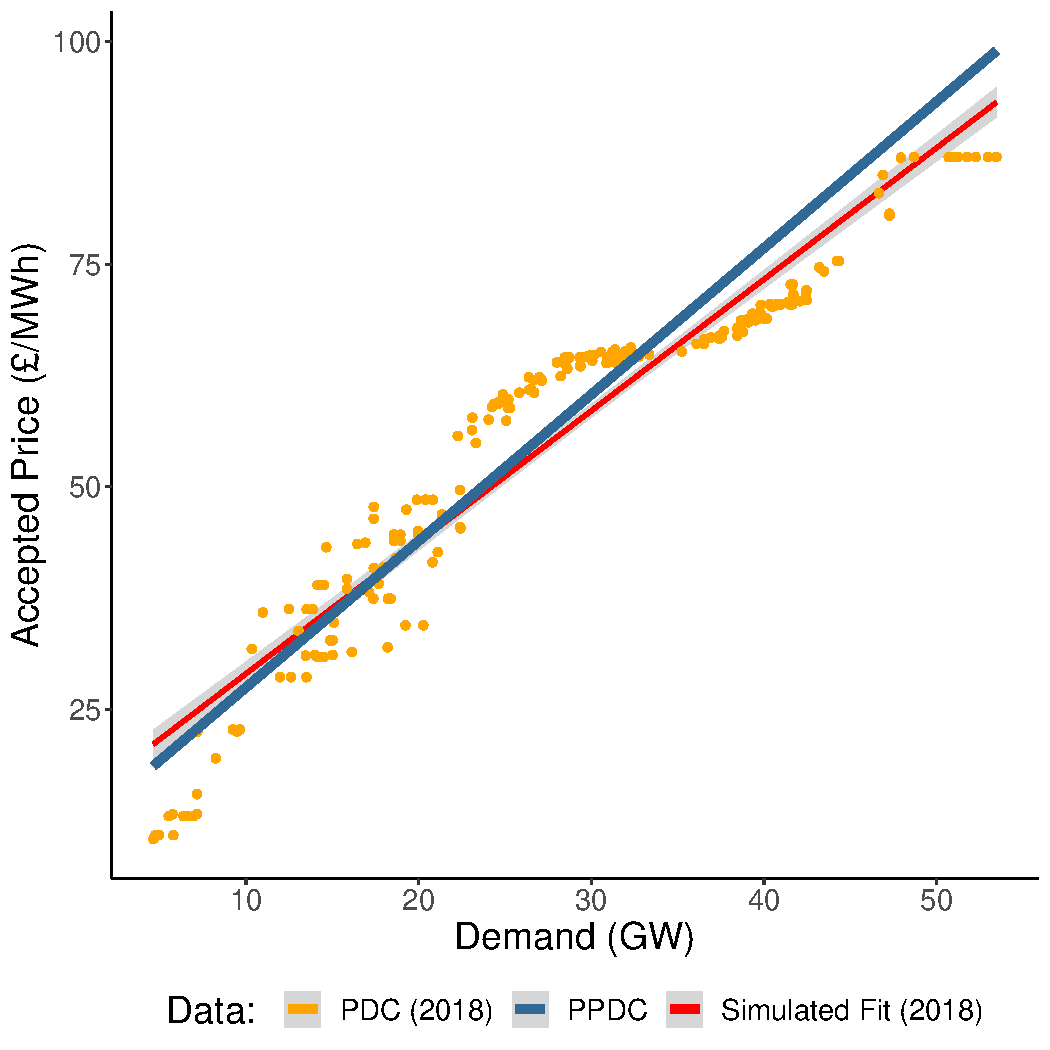
\includegraphics[width=0.65\textwidth]{Chapter4/figures/e-Energy-2020/results/best_run_price_dur_curve.pdf}
	\caption{Predicted price duration curve for investment for most accurate run against simulated run in 2018.}
	\label{fig:best_price_curve}
\end{figure}

The yellow points show the simulated price duration curve for the first year of the simulation (2018). The red line (Simulated Fit (2018)) is a linear regression that approximates the simulated price duration curve (PDC (2018)). The blue line shows the price duration curve predicted ($PPDC$) by the GenCos to be representative of the expected prices over the lifetime of the plant.

%The blue line is the price duration curve simulated in 2018, and the red line is the optimal predicted electricity mix. 

The optimal predicted price duration curve ($PPDC$) closely matches the simulated fit in 2018, shown by Figure \ref{fig:best_price_curve}. However, the $PPDC$ has a slightly higher peak price and lower baseload price. This could be due to the fact that there is a predicted increase in the number of renewables with a low SRMC. However, due to the intermittency of renewables such as solar and wind, higher peak prices are required to generate in times of low wind and solar irradiance at the earth's surface.






To generate Figure \ref{fig:uk_validated_results_2018}, we ran 40 scenarios with the $PPDC$ to observe the final, simulated electricity mix. The error bars are computed based on a Normal distribution 95\% confidence interval.

ElecSim was able to model the increase in renewables and stability of nuclear energy in this time. ElecSim was also able to model the transition from coal to gas, however, underestimated the magnitude of the transition. This was similar to the projections BEIS made in 2013 as previously discussed.

\begin{figure}
	\centering
	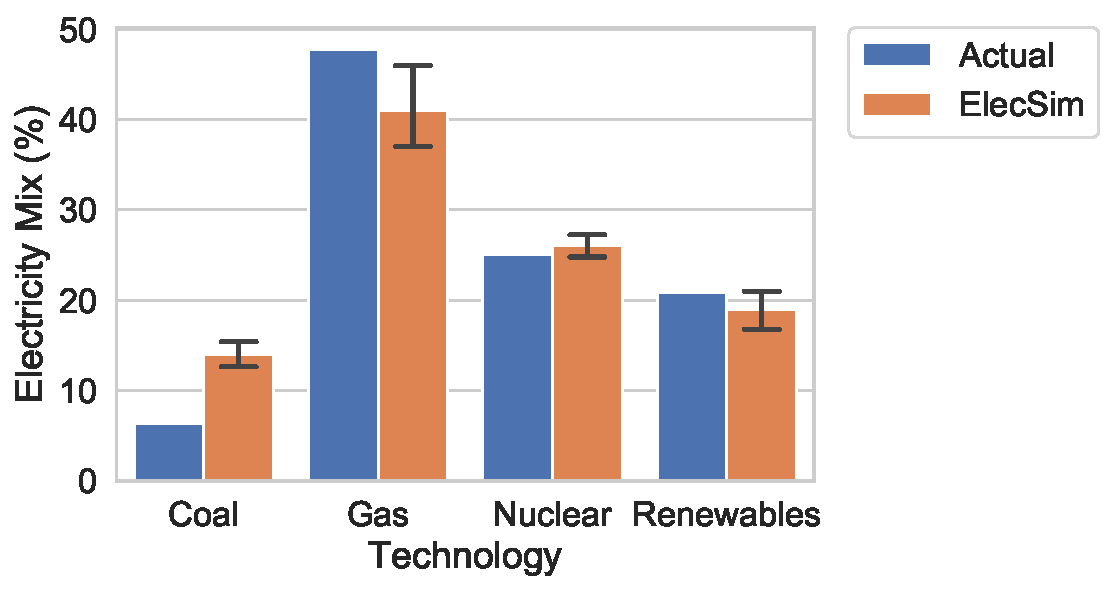
\includegraphics[width=0.65\textwidth]{Chapter4/figures/e-Energy-2020/results/best_run_coal_dropout_95_ci.pdf}
	\caption{Electricity generation mix simulated by ElecSim from 2013 to 2018 compared to observed electricity mix in 2018.}
	\label{fig:uk_validated_results_2018}
\end{figure}

%Figure \ref{fig:single_time_step_results} displays the results using the same scenario details such as fuel and carbon price, electricity generation costs and GenCos. As mentioned in Section \ref{ssec:representative_days}, we see an overestimation in the uptakes of IRES. In this case all electricity sources are replaced by wind which with current storage technologies is not possible.



%\begin{figure}
%\centering
%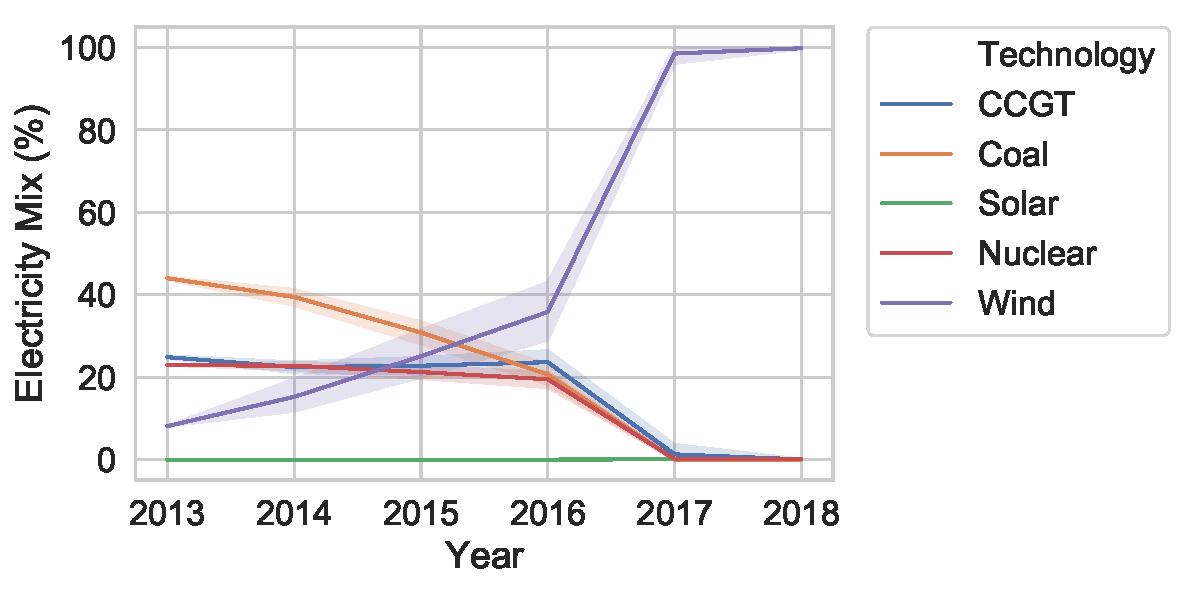
\includegraphics[width=0.49\textwidth]{figures/results/yearly_time_step_scenario.pdf}
%\caption{Electricity mix actual vs. simulated for validation scenario with a single representative day.}
%\label{fig:single_time_step_results}
%\end{figure}



\subsubsection{Long-Term Scenario Analysis}

In this section we discuss the results of the analysis of the BEIS reference scenario explained in Section \ref{sssec:scen-analysis}. Specifically, we created a scenario that mimicked that of BEIS in ElecSim and optimised a number of parameters using a genetic algorithm to match this scenario. Through this we are able to gain confidence in the underlying dynamics of ElecSim to simulate long-term behaviours. Further, this enables us to verify the likelihood of the scenario by analysing whether the parameters required to make such a scenario are realistic.

Figure \ref{fig:forward_scenario_beis_elecsim} displays the electricity mix projected by both ElecSim and BEIS. To generate this image we ran 60 scenarios under the optimal collection of predicted price duration curves, nuclear subsidy and uncertainty in predicted price duration curves. 

The optimal parameters were chosen by choosing the parameter set with the lowest mean error per electricity generation type and per year throughout the simulation, as shown by Equation \ref{eq:long-term-reward}.


Figure \ref{fig:forward_scenario_best_pdcs} displays the optimal predicted price duration curves ($PPDC$s) per year of the simulation, shown in blue. These are compared to the price duration curve simulated in 2018, as per Figure \ref{fig:best_price_curve}. The optimal nuclear subsidy, $S_n$, was found to be ${\sim}$\textsterling $120$, the optimal $\sigma_m$ and $\sigma_c$ were found to be $0$ and ${\sim}0.0006$ respectively.

The BEIS scenario demonstrates a progressive increase in nuclear energy from 2025 to 2035, a consistent decrease in electricity produced by natural gas, an increase in renewables and decrease to almost 0\% by 2026 of coal.

ElecSim is largely able to mimic the scenario by BEIS. A large increase in renewables is projected, followed by a decrease in natural gas. 

A significant difference, however, is the step-change in nuclear power in 2033. This led to an almost equal reduction in natural gas during the same year. In contrast, BEIS project a continuously increasing share of nuclear. 

We argue that the ElecSim projection of nuclear power is more realistic than that of BEIS due to the instantaneous nature of large nuclear power plants coming on-line.

Figure \ref{fig:forward_scenario_best_pdcs} exhibits the price curves required to generate the scenario show in Figure \ref{fig:forward_scenario_beis_elecsim}. The majority of the price curves are similar to the simulated price duration curve of 2018 (Simulated Fit (2018)). However, there are some price curves which are significantly higher and significantly lower than the predicted price curve of 2018. These cycles in predicted price duration curves may be explained by investment cycles typically exhibited in electricity markets \cite{Gross2007}. 

In this context, investment cycles reflect a boom and bust cycle over long timescales. When electricity supply becomes tight relative to demand, prices rise to create an incentive to invest in new capacity. Price behaviour in competitive markets can lead to periods of several years of low prices (close to short-run marginal cost) \cite{white2005concentrated}. 

As plants retire or demand increases, the market becomes tighter until average prices increase to a level above the threshold for investment in new power generators. At this point investors may race to bring new plants on-line to make the most out of the higher prices. Once adequate investments have been made, the market returns to a period of low prices and low investment until the next price spike \cite{Gross2007}. 


The nuclear subsidy, $S_n$, of ${\sim}$\textsterling $120$ in 2018 prices is high compared to similar subsidies, but this may reflect the difficulty of nuclear competing with renewable technology with a short-run marginal cost that tends to \textsterling $0$.

The low values of $\sigma_m$ and $\sigma_c$ demonstrates that the expectation of prices does not necessarily have to differ significantly between GenCos. This may be due to the fact that GenCos have access to the same market information.


\begin{figure}
	\centering
	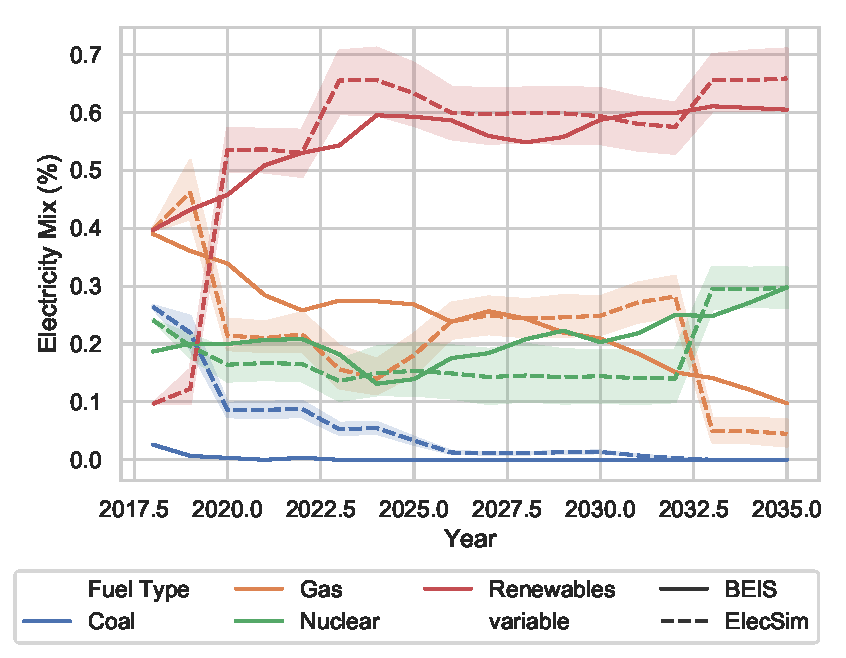
\includegraphics[width=0.60\textwidth]{Chapter4/figures/e-Energy-2020/results/scenario_analysis/best_forward_scenario_below_legend.pdf}
	\caption{Comparison of ElecSim and BEIS' reference scenario from 2018 to 2035.}
	\label{fig:forward_scenario_beis_elecsim}
\end{figure}



\begin{figure}
	\centering
	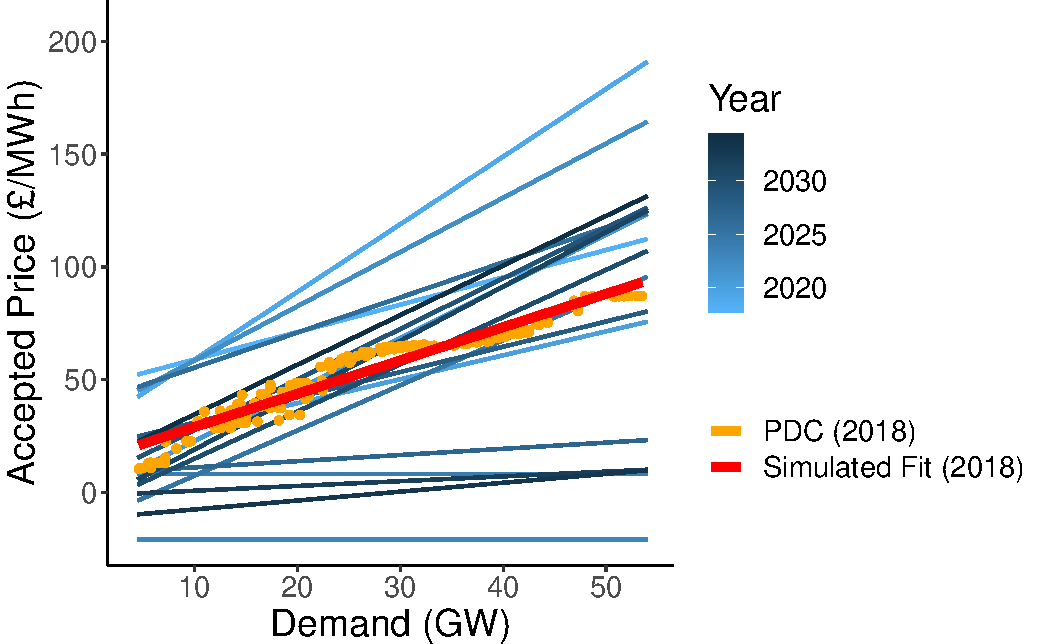
\includegraphics[width=0.6\textwidth, keepaspectratio]{Chapter4/figures/e-Energy-2020/results/scenario_analysis/optimal_pdc_prices.pdf}
	\caption{Comparison between optimal price duration curves and simulated price duration curve in 2018.}
	\label{fig:forward_scenario_best_pdcs}
\end{figure}


%\begin{figure}
%\centering
%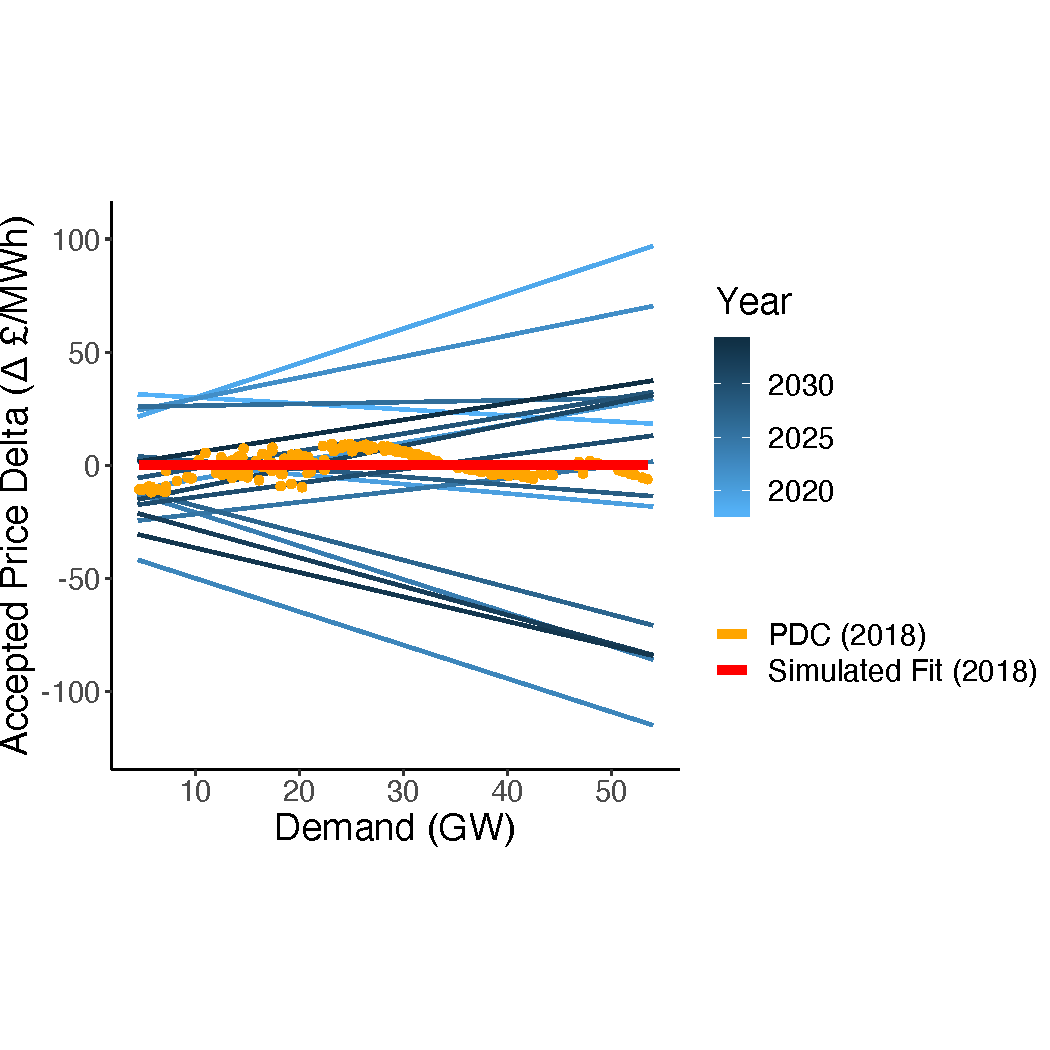
\includegraphics[width=0.49\textwidth, height=0.49\textwidth, keepaspectratio]{figures/results/scenario_analysis/optimal_pdc_prices_differences_delta.pdf}
%\caption{Comparison between optimal price duration curves and simulated price duration curve in 2018.}
%\label{fig:forward_scenario_best_pdcs}
%\end{figure}




\clearpage
\section{Scenario Testing}
\label{elecsim:sec:scenarios}

In this Section we display scenario runs of ElecSim using 20 time-steps per year and using representative days

\subsection{Scenarios for 20 time-steps}

In this section we present example scenario runs using ElecSim with 20 time-steps. We vary the carbon tax and grow or reduce total electricity demand. This enables us to observe the effects of carbon tax on investment. In this paper, we have presented scenarios where electricity demand decreases 1\% per year, due to the recent trend in the UK.

%ElecSim was built using python, this enabled us to lower barriers to entry and allow for users to integrate state-of-the-art machine learning and statistical packages in future work. We used project mesa as an open source agent based modelling framework for its ease of use \cite{Masad2015}.

% {\color{blue}
% We assume that carbon tax is set by the government, and not subject to market forces such as the EU Emissions Trading Scheme \cite{Council2016}.

% We run 16 different scenarios 8 times each, with demand increasing and decreasing by 1\% per year and  varying carbon prices. In this section we explore a decreasing demand of 1\% a year. We chose this due to the increasing efficiency of homes, industry and technology, and due to the recent trend in the UK. Demand, however, did not display a large effect on the optimum carbon price. We select a burn-in period of 6 years, due to the fact that the majority of power plants take 6 years to go from investment to operation.

% Table \ref{table:scenario_statistics}, in the appendix, displays the summary statistics of each run.

% It can be seen from Figure \ref{fig:demand99carbon10} that a carbon tax of \textsterling10 per year does little to influence investment in low-carbon, renewable technology. With traditional, fossil fuel based generation, providing the majority of supply in each year. However, there is an increase in renewable technology over the years, starting from mean 15.85\% market share in the year range 2019-2029, to 24.38\% in the year range 2039-2050. A similar increase of renewable energy with a carbon tax of \textsterling0 can be seen, albeit at a lower mean by the year range 2039-2050 (22.29\%).
% }

For the first scenario run displayed, we have approximated the predictions by the UK Government, where carbon tax increases linearly from \textsterling18 to \textsterling200 by 2050 \cite{Department2016}. Figure \ref{fig:demand99carbon18} demonstrates a significant increase in gas turbines in the first few years, followed by a decrease, with onshore wind increasing.

Figure \ref{fig:demand99carbon40} displays a run with a \textsterling40 carbon tax. This run demonstrates a higher share of onshore wind than in the previous scenario. 

We experimented with the following levels of carbon tax: \textsterling10 (\$13), \textsterling20 (\$26) and \textsterling70 (\$90) with demand decreasing 1\% per year. This was chosen due to the increasing efficiency of homes, industry and technology, and due to the recent trend in the UK. We run each scenario 8 times to capture the stochastic nature of the process. Via the observation of the emergent investment behaviour until 2050, an understanding of how real life investors may behave emerges.


Figure \ref{fig:demand99carbon10} shows that with a carbon tax of \textsterling10, whilst renewable technology does grow, gas power plants provide the majority of supply in each year. However, at a level of \textsterling20 the increase in wind turbines is enough to match gas turbines. A carbon tax of \textsterling70, however, shows a near 100\% uptake of wind turbines.

It is infeasible for the power supply to be provided solely by wind turbines today. This overestimation, however, is due to the low time granularity of the model \cite{Collins2017}. This scenario therefore assumes perfect storage capabilities.



These runs demonstrate that a consistent, but relatively low carbon tax can have a larger impact in the uptake of renewable energy than increasing carbon tax over a long time frame. We hypothesise that an early carbon tax affects the long-term dynamics of the market for many years. We, therefore, suggest early action on carbon tax to transition to a low-carbon energy supply


%The UK Government BEIS have predicted a carbon tax increasing from \textsterling18 to \textsterling200 by 2050, with carbon price increasingly linearly from 2030 to 2050 \cite{Department2016}. We have approximated these assumptions and modelled the results, shown by Figure \ref{fig:demand99carbon18}. The results show only a slight decrease in low-carbon supply over the \textsterling40 carbon tax energy mix. This demonstrates the importance of long-term modelling, and understanding the long-term impacts that can result. It is hypothesised that a lower carbon tax early on changes the market dynamics for years to come, due to certain price structures.
%
%Figure \ref{fig:demand99carbon40} shows that a carbon tax of \textsterling40 is sufficient in moving towards a low-carbon economy, with backup fossil fuel generators.

% {\color{blue}However, by referring to Figure \ref{fig:demand99carbon70} it can be seen that to have 100\% renewable, a carbon price of \textsterling70 is required.

% These results show the importance of making difficult decisions as soon as possible to have the biggest effect on the energy mix for years to come.}

% \begin{figure}
% \begin{center}
% 		\includegraphics[width=0.5\textwidth]{figures/scenarios/demand099-carbon70-datetime.png}
% 		\caption{{\color{blue}Demand decreasing by 1\% per year with a carbon tax of \textsterling70.}}
% 		\label{fig:demand99carbon70}
% 	\end{center}
% \end{figure}



% \begin{figure*}[h]
% 	\centering
% 	\begin{subfigure}[b]{0.475\textwidth}
% 		\centering
% 		\includegraphics[width=\textwidth]{figures/scenarios/demand099-carbon10-datetime.png}
% 		\caption[Network2]%
% 		{{{\color{blue}{\small \textsterling10 carbon tax.}}}}
% 		\label{fig:demand99carbon10}
% 	\end{subfigure}
% 	\hfill
% 	\begin{subfigure}[b]{0.475\textwidth}  
% 		\centering 
% 		\includegraphics[width=\textwidth]{figures/scenarios/demand099-carbon20-datetime.png}
% 		\caption[]%
% 		{{{\color{blue}\textsterling20 carbon tax.}}}
% 		\label{fig:demand99carbon20}
% 	\end{subfigure}
% 	\vskip\baselineskip

%
%	\begin{subfigure}[b]{0.475\textwidth}   
%		\centering 
%		\includegraphics[width=\textwidth]{figures/scenarios/demand099-carbon18-datetime.png}
%		\caption[]%
%		{{\textsterling26 to \textsterling150 linearly increasing carbon tax.}}    
%		\label{fig:demand99carbon18}
%	\end{subfigure}
%	\quad
%	\begin{subfigure}[b]{0.475\textwidth}   
%		\centering 
%		\includegraphics[width=\textwidth]{figures/scenarios/demand099-carbon40-datetime.png}
%		\caption[]%
%		{{\textsterling40 carbon tax.}}    
%		\label{fig:demand99carbon40}
%	\end{subfigure}
%	\caption[ Scenarios up to the year 2050 with varying carbon taxes and decreasing demand ]
%	{\small Scenarios up to the year 2050, with varying carbon taxes and electricity demand decreasing 1\% a year.} 
%	\label{fig:mean and std of nets}
%\end{figure*}
%\FloatBarrier

%\begin{figure}[b]{0.475\columnwidth}   
%	\centering 
%	\includegraphics{figures/scenarios/demand099-carbon18-datetime.png}
%	\caption[]%
%	{{\textsterling26 to \textsterling150 linearly increasing carbon tax.}}    
%	\label{fig:demand99carbon18}
%\end{figure}
%
%\begin{figure}[b]{0.475\columnwidth}   
%	\centering 
%	\includegraphics{figures/scenarios/demand099-carbon40-datetime.png}
%	\caption[]%
%	{{\textsterling40 carbon tax.}}    
%	\label{fig:demand99carbon40}
%\end{figure}

\begin{figure}
	\centering
	\begin{subfigure}{.7\linewidth}
		\includegraphics[width=0.6\linewidth]{Chapter4/figures/scenarios/demand099-carbon18-datetime.png}
		\caption{\textsterling26 to \textsterling150 linearly increasing carbon tax.}
		\label{fig:demand99carbon18}
	\end{subfigure}
	\begin{subfigure}{.7\linewidth}
		\includegraphics[width=0.6\linewidth]{Chapter4/figures/scenarios/demand099-carbon40-datetime.png}
		\caption{{\textsterling40 carbon tax}}
		\label{fig:demand99carbon40}
	\end{subfigure}
	\caption{Scenarios with varying carbon taxes and decreasing demand (-1\%/year)}
\end{figure}






%\begin{figure}[h]
%	\begin{center}
%		\includegraphics[width=0.5\textwidth]{figures/scenarios/demand099-carbon10-datetime.png}
%		\caption{Demand decreasing by 1\% per year and a carbon tax of \textsterling10}
%		\label{fig:demand99carbon10}
%	\end{center}
%\end{figure}
%
%\begin{figure}[h]
%	\begin{center}
%		\includegraphics[width=0.5\textwidth]{figures/scenarios/demand099-carbon20-datetime.png}
%		\caption{Demand decreasing by 1\% per year and a carbon tax of \textsterling20}
%		\label{fig:demand99carbon10}
%	\end{center}
%\end{figure}
%
%
%
%\begin{figure}[h]
%	\begin{center}
%		\includegraphics[width=0.5\textwidth]{figures/scenarios/demand099-carbon18-datetime.png}
%		\caption{Demand decreasing by 1\% per year and a carbon tax of \textsterling20}
%		\label{fig:demand99carbon10}
%	\end{center}
%\end{figure}
%
%
%
%\begin{figure}[h]
%	\begin{center}
%		\includegraphics[width=0.5\textwidth]{figures/scenarios/demand099-carbon40-datetime.png}
%		\caption{Demand decreasing by 1\% per year and a carbon tax of \textsterling20}
%		\label{fig:demand99carbon10}
%	\end{center}
%\end{figure}
%\begin{figure}
%	\centering
%	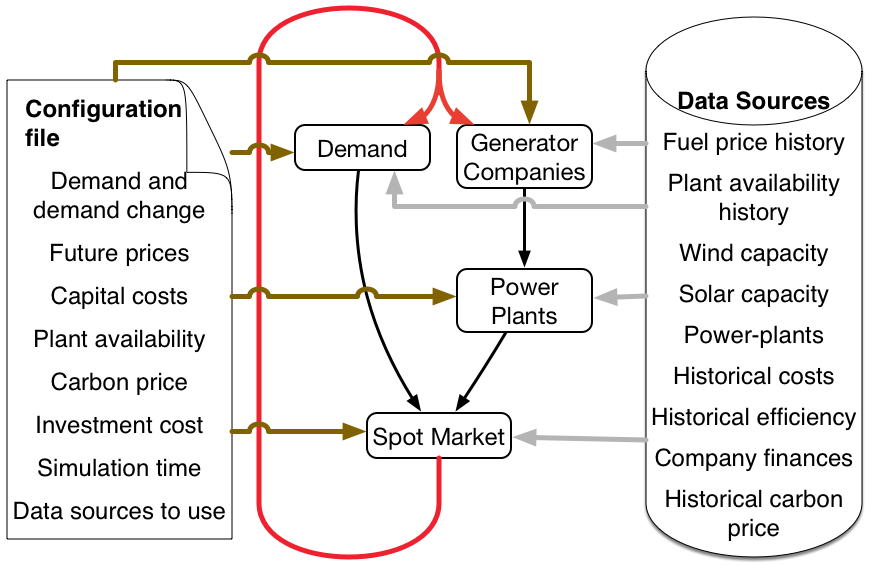
\includegraphics[width=0.85\linewidth]{Chapter4/figures/System_overview_large}
%	\caption{System overview of agent-based market model.}
%	\label{fig:systemoverview}
%	\vskip -6mm
%\end{figure}


\begin{figure}[h]
	\centering
	\begin{subfigure}[b]{0.6\textwidth}
		\centering
		\includegraphics[width=\textwidth]{Chapter4/figures/scenarios/demand099-carbon10-datetime.png}
		\caption[Network2]%
		{\small \textsterling10 carbon tax.}
		\label{fig:demand99carbon10}
	\end{subfigure}
	\hfill
	\begin{subfigure}[b]{0.6\textwidth}  
		\centering 
		\includegraphics[width=\textwidth]{Chapter4/figures/scenarios/demand099-carbon20-datetime.png}
		\caption[]%
		{\textsterling20 carbon tax.}
		\label{fig:demand99carbon20}
	\end{subfigure}
	\begin{subfigure}[b]{0.6\textwidth}
		\centering
		\includegraphics[width=\textwidth]{Chapter4/figures/scenarios/demand099-carbon70-datetime.png}
		\caption[Network2]%
		{\small \textsterling70 carbon tax.}
		\label{fig:demand99carbon70}
	\end{subfigure}
	\caption{Scenarios from 2020 to 2050 with varying carbon tax.}
\end{figure}









\subsection{Conclusion}


Agent-based models provide a method of simulating investor behaviour in an electricity market. We observed that an increase in carbon tax had a significant impact on investment. These findings enable policy makers to better understand the impact that their decisions may have. For a high uptake of renewable energy technology, rapid results can be seen after 10 years with a carbon tax of \textsterling70 (\$90).




\subsection{Scenarios for representative days}

In this section we discuss various scenarios under the model which uses representative days as time-steps. This work builds upon the work in Section \ref{architecture:sec:validation}; we used the same predicted price duration curves as modelled on BEIS' scenario. We selected an optimal carbon tax level which would reduce both electricity price and carbon emissions, as shown later in Chapter \ref{chapter:carbon}. The optimal carbon tax strategy found in Chapter \ref{chapter:carbon} is shown by Figure \ref{elecsim:fig:optimal_carbon_tax_strategy}. Each of the scenarios were run 10 times to display any variability in the results. We chose 10 runs to limit both computation time and cost.



\begin{figure}
	\centering
	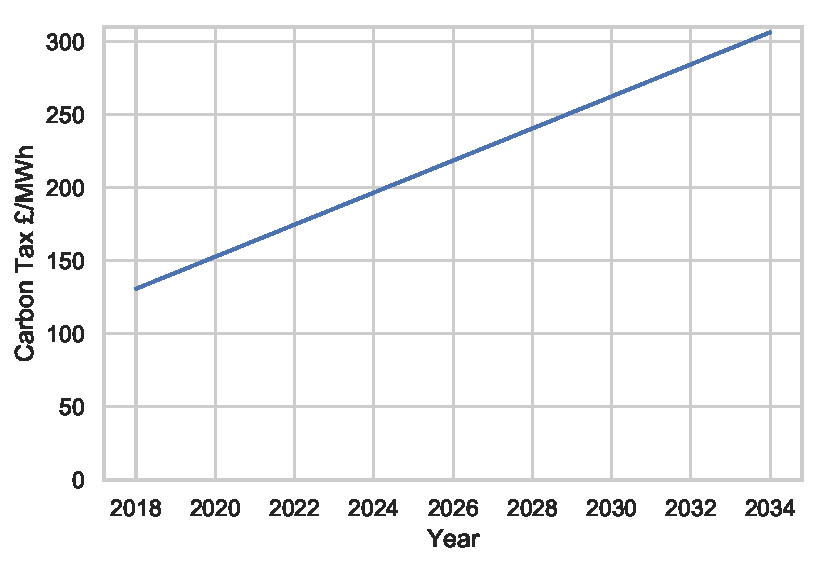
\includegraphics[width=0.7\textwidth, keepaspectratio]{Chapter4/figures/scenarios/representative-day-scenarios/optimal_carbon_strategy.pdf}
	\caption{Optimal carbon tax strategy to reduce both electricity cost and carbon emissions.}
	\label{elecsim:fig:optimal_carbon_tax_strategy}
\end{figure}

Figures \ref{elecsim:fig:increasing_demand} and \ref{elecsim:fig:decreasing_demand} show the electricity mixes of various demand scenarios. Figure \ref{elecsim:fig:increasing_demand} displays the scenarios in which demand either stays flat, or decreases by 1\% and 2\%. For these scenarios it can be seen that solar is the dominant electricity supply, supplying ${\sim}$50\%, with nuclear power in second supplying between 20\% and 30\%. With a decreasing demand scenario of 1\% per year, as shown by Figure \ref{fig:demand099}, nuclear provides a higher proportion by the year 2034, of ${\sim}$30\%, however before the year 2033, provides a similar proportion to the other scenarios as shown by Figures \ref{fig:demand10} and \ref{fig:demand098}.

For the scenarios shown in Figure \ref{elecsim:fig:increasing_demand}, CCGT, coal and onshore provide around ${\sim}$10\% each by 2034.  Coal and CCGT, however, progress towards 0\% whereas onshore wind increases. This is to be expected due to the high carbon price, as shown by Figure \ref{elecsim:fig:optimal_carbon_tax_strategy}. Offshore does not exhibit a high amount of investment. We believe this is the case as offshore wind is more expensive than onshore wind, and in our scenario subsidies other than for nuclear are not modelled.

\begin{figure}
	\centering
	\begin{subfigure}{0.6\textwidth}
		\centering
		
\includegraphics[width=\textwidth]{Chapter4/figures/scenarios/representative-day-scenarios/10_demand_mix.pdf}
		\caption{Demand does not increase or decrease.}
		\label{fig:demand10}
	\end{subfigure}
	\hfill
	\begin{subfigure}{0.6\textwidth}  
		\centering 
		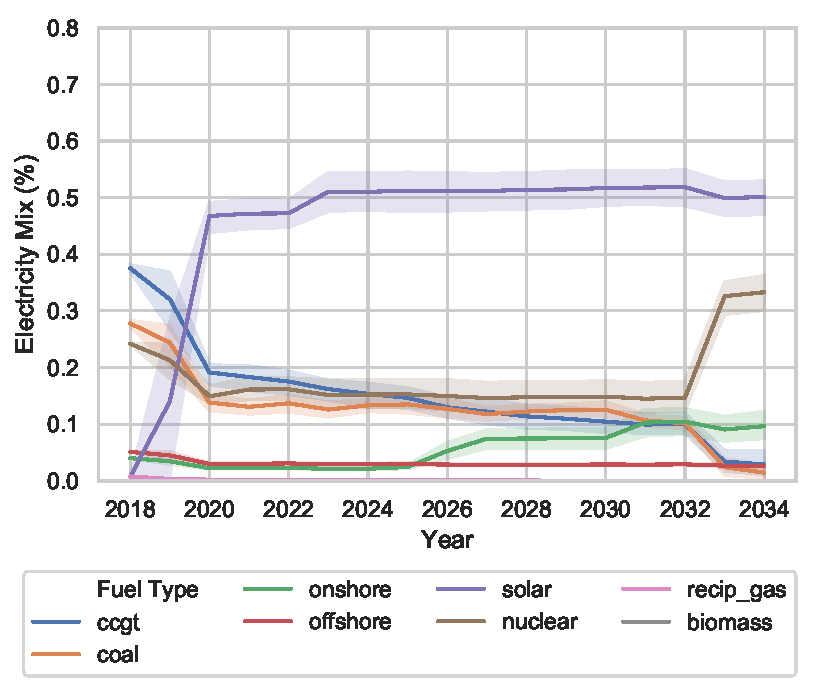
\includegraphics[width=\textwidth]{Chapter4/figures/scenarios/representative-day-scenarios/099_demand_mix.pdf}
		\caption{Demand reduces by 1\% per year.}
		\label{fig:demand099}
	\end{subfigure}
	\begin{subfigure}{0.6\textwidth}
		\centering
		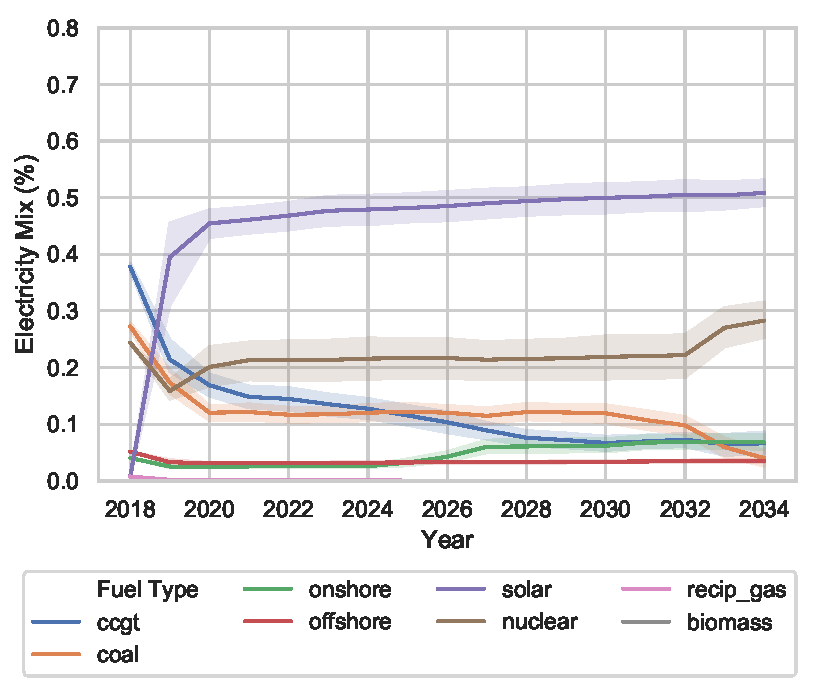
\includegraphics[width=\textwidth]{Chapter4/figures/scenarios/representative-day-scenarios/098_demand_mix.pdf}
		\caption{\small Demand reduces by 2\% per year}
		\label{fig:demand098}
	\end{subfigure}
	\caption{Scenarios from 2018 to 2035 with varying demand.}
	\label{elecsim:fig:increasing_demand}
\end{figure}


Figure \ref{elecsim:fig:decreasing_demand} shows scenarios where demand increases per year. Whilst electricity mix distribution is similar to the scenarios shown in Figure \ref{elecsim:fig:increasing_demand}, solar plays a significantly increased role than nuclear. This may be down to the large expense of nuclear, and the long time of deployment of this type of technology. Solar power, on the other hand, is able to be installed much more quickly to maintain the high demand. This is especially true for the scenarios shown in Figures \ref{fig:demand102} and \ref{fig:demand1025} where demand rises by 2\% and 2.5\% per year respectively. 



\begin{figure}
	\centering
	\begin{subfigure}{0.6\textwidth}
		\centering
		
\includegraphics[width=\textwidth]{Chapter4/figures/scenarios/representative-day-scenarios/101_demand_mix.pdf}
		\caption{\small Demand increases by 1\% per year.}
		\label{fig:demand101}
	\end{subfigure}
	\hfill
	\begin{subfigure}{0.6\textwidth}  
		\centering 
		
\includegraphics[width=\textwidth]{Chapter4/figures/scenarios/representative-day-scenarios/102_demand_mix.pdf}
		\caption{\small Demand increases by 2\% per year.}
		\label{fig:demand102}
	\end{subfigure}
	\begin{subfigure}{0.6\textwidth}
		\centering
		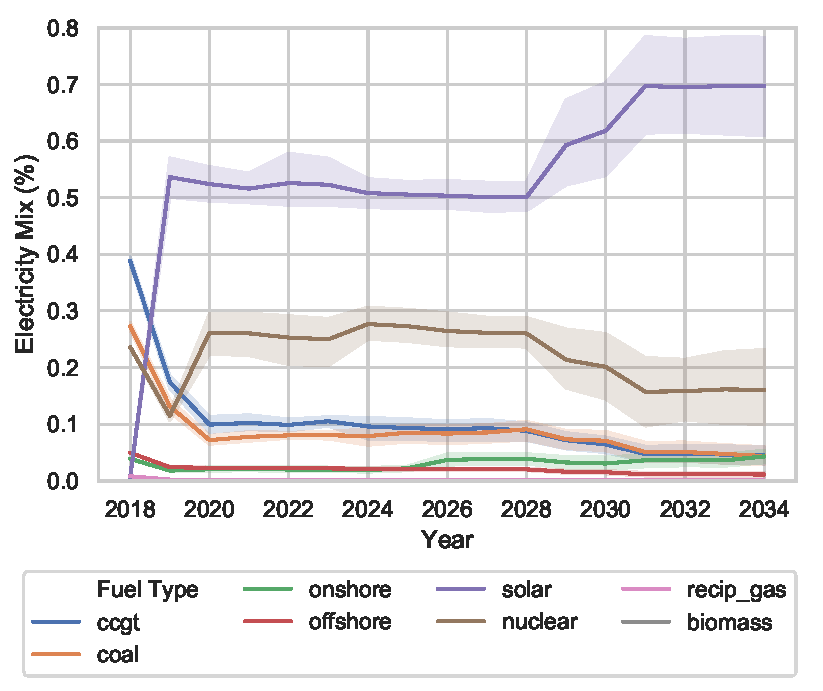
\includegraphics[width=\textwidth]{Chapter4/figures/scenarios/representative-day-scenarios/1025_demand_mix.pdf}
		\caption{\small Demand increases by 2.5\% per year}
		\label{fig:demand1025}
	\end{subfigure}
	\caption{Scenarios from 2018 to 2035 with varying demand.}
	\label{elecsim:fig:decreasing_demand}
\end{figure}























\subsection{Performance}


\begin{figure}
	\centering
	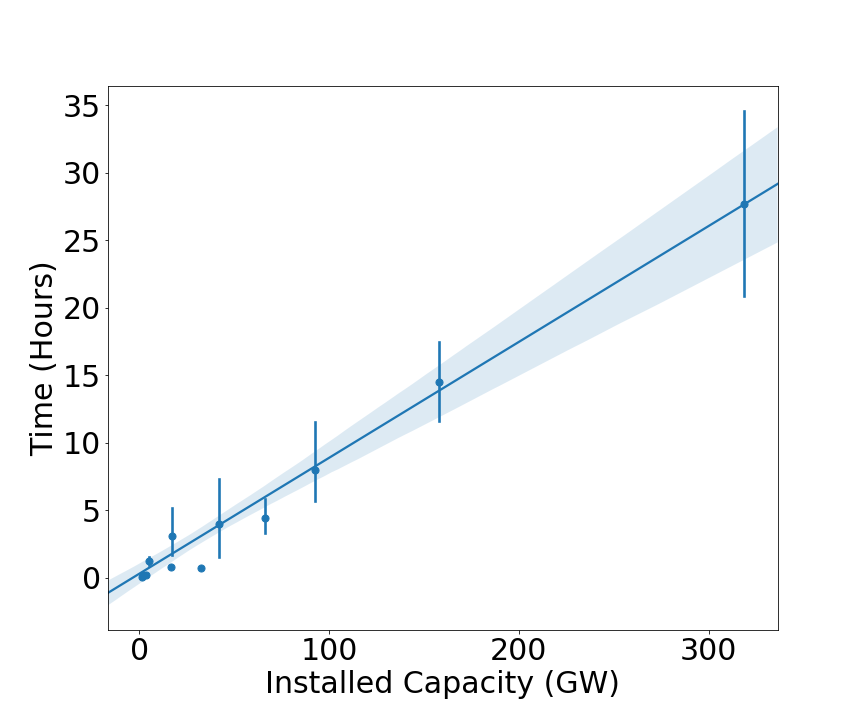
\includegraphics[width=0.6\linewidth]{Chapter4/figures/timing_plot.png}
	\caption{Run times of different sized countries.}
	\label{fig:timingplot}
	\vskip -0.5cm
\end{figure}


Figure \ref{fig:timingplot} shows the running time for ElecSim with varying installed capacity. We varied demand between 2GW and 320GW to see the effect of different sized countries on running time. The makeup of the electricity mix was achieve through stratified sampling of the UK electricity mix. The results show a linear time complexity. 


%\begin{itemize}
%	\item Validation of model 
%	\begin{itemize}
%		\item Compare price duration curve
%		\item Compare power plant costs and NPV calculations
%		\item Look number of steps ahead to compare electricity mix and compare to actual (cross-validation)
%	\end{itemize} 
%	\item Performance metrics - Comparison with EMLab, PowerACE (15 minute run time)
%	\begin{itemize}
%		\item Memory, disk size, runtime
%		\item Increase in time complexity with additional data.
%	\end{itemize}
%\end{itemize}



\clearpage
\section{Sensitivity Analysis}
\label{elecsim:sec:sensitivity}

In this section we investigate a sensitivity analysis of ElecSim, where we vary the weighted average cost of capital and the down payment required for investment. We used the reference scenario discussed in Section \ref{elecsim:sec:scenarios}, with the optimal carbon tax to reduce both emissions and electricity price. The work done in this Section is in addition to the work published in \cite{Kell2020}.

We ran ten iterations per weighted average cost of capital and down payment element. We did this due to the monte-carlo nature of the simulation. We chose ten runs to give us sufficient variance in results, but reduce compute power, to reduce both time and cost of calculation.

\subsection{Results}

Figure \ref{elecsim:fig:wacc_sensitivity} displays the results of the sensitivity analysis for the \Gls{WACC} for non-nuclear power generators. For this, we trialled nine different \acrfull{wacc} values, where a value of 5.9\% is the reference case \cite{KincheloeStephenC1990TWAC}. 

It can be seen that the \acrshort{wacc} has an effect on the total investment in solar, nuclear and CCGT. With a \acrshort{wacc} equal to or greater than 7.4\%, nuclear increases significantly, whilst solar decreases. Nuclear has a \acrshort{wacc} of 10\%, therefore 7.4\% may be the point where nuclear becomes more competitive than solar in an environment where a low-carbon electricity supply is elicited from an optimal carbon tax.

Offshore and coal do not change significantly over different levels of \acrshort{wacc}. This may be due to the fact that CCGT and onshore are more competitive than coal and offshore respectively, without external subsidies. 

Onshore seems to play a larger role at the lowest \acrshort{wacc}, 3.9\%. This may be due to onshore wind's high competitiveness when compared to nuclear.



\begin{figure}
	\centering
	\includegraphics[width=0.9\linewidth]{Chapter4/figures/sensitvity_analysis/wacc_sensitivity_analysis.pdf}
	\caption{Sensitivity analysis where \acrfull{wacc} was varied. Results compare electricity mix in 2035.}
	\label{elecsim:fig:wacc_sensitivity}
\end{figure}

Figure \ref{elecsim:fig:wacc_carbon_sensitivity} displays the relative carbon emissions in 2035. With a low \acrshort{wacc} of 3.9\%, the relative carbon emissions falls, on average, to zero. This seems to be due to the high levels of solar, onshore and nuclear.  

As \acrshort{wacc} increases, so does carbon emissions, until there is a \acrshort{wacc} of 0.5, where it reduces slightly. This is seemingly due to the higher levels of CCGT and coal, which is able to displace solar. However, it must be noted, that in this scenario with the optimal carbon tax, the relative carbon emissions remains low. 


\begin{figure}
	\centering
	\includegraphics[width=0.9\linewidth]{Chapter4/figures/sensitvity_analysis/wacc_carbon_sensitivity_analysis.pdf}
	\caption{Sensitivity analysis where weighted average cost of capital (WACC) was varied. Results compare relative carbon emissions in 2035.}
	\label{elecsim:fig:wacc_carbon_sensitivity}
\end{figure}

Figure \ref{elecsim:fig:downpayment_sensitivity} displays the sensitivity analysis results for different levels of down payment required for all investments. We varied the down payment required between the values of 10\% and 40\%.

As down payment required increases, so does nuclear and onshore, whilst solar decreases. CCGT also shows an increase with down payment required. The increase in down payment may help nuclear, due to the high costs of \acrshort{wacc}. With a higher down payment, the total costs of the project will fall when compared to other, cheaper, generators. It is likely that nuclear displaces solar in this case. CCGT increases up until a 35\% down payment required. This may be due to the increased use of onshore wind, where CCGT and coal is required to fill for times of low wind speeds.

 

\begin{figure}
	\centering
	\includegraphics[width=0.9\linewidth]{Chapter4/figures/sensitvity_analysis/downpayment_sensitivity_analysis.pdf}
	\caption{Sensitivity analysis where percentage of down payment was varied. Results compare electricity mix in 2035.}
	\label{elecsim:fig:downpayment_sensitivity}
\end{figure}

Figure \ref{elecsim:fig:downpayment_carbon_sensitivity} displays the relative carbon emissions versus down payment required for investors. As down payment increases, so does relative carbon emissions. This is down to the increasing role that CCGT and coal play in the electricity mix, and decreasing solar capacity. 

A down-payment of 10\% seems to have the lowest carbon emissions. This is due to the high investment in solar, and low investment in CCGT and coal. 

\begin{figure}
	\centering
	\includegraphics[width=0.9\linewidth]{Chapter4/figures/sensitvity_analysis/downpayment_carbon_sensitivity_analysis.pdf}
	\caption{Sensitivity analysis where percentage of down payment was varied. Results compare relative carbon emissions in 2035.}
	\label{elecsim:fig:downpayment_carbon_sensitivity}
\end{figure}


\section{Limitations}
\label{elecsim:sec:limitations}
% Requirement of exogeneous price prediction curve
% Inability to validate on a long-term basis
% Lack of detailed supply curves (such as maximum wind and solar irradiance)
% Comparing to other models may not be correct as all models are wrong
% Future may change dramatically
% Lack of contracts for difference modelling and other subsidies (apart from nuclear)



\clearpage
\section{Conclusions}
\label{elecsim:sec:conclusions}

%%%%%%%%%%%%%%%%%%%%%%%%%%%%%%%%%%%%%%%%%%%%%%%%
%%%%%%%%%%%%%%%%%%%%%%%%      Paper 1    %%%%%%%%%%%%%%%%
%%%%%%%%%%%%%%%%%%%%%%%%%%%%%%%%%%%%%%%%%%%%%%%%

Liberalised electricity markets with many heterogeneous players are suited to be modelled with ABMs. ABMs incorporate imperfect information as well as heterogeneous actors. ElecSim models imperfect information through forecasting of electricity demand and future fuel and electricity prices. This leads to agents taking risk on their investments, and model market conditions more realistically.

%We demonstrated that increasing carbon tax can lead to an increase in investment of low-carbon technologies. We showed that early decisions have a long-term impact on the energy mix. 

%Our future work includes comparing agent-learning techniques, using multi-agent reinforcement learning algorithms to allow agents to learn in a non-static environment. We propose the integration of a higher temporal and spatial resolution to model changes in daily demand, as well as capacity factors by region, and transmission effects. This will allow us to model that demand is met at all times and not just on average. 
%\begin{itemize}
%	\item Requirement for agent based models based on imperfect information, liberalised energy markets
%	\item Requirement for low barriers to entry open source model.
%	\item Discuss results
%	\item Future work:
%	\begin{itemize}
%		\item Embedding multi-agent intelligence such as Genetic Algorithms,  Q-learning and dynamic reinforcement learning
%		\item Raise spatial and temporal resolution.
%	\end{itemize}
%\end{itemize}



%%%%%%%%%%%%%%%%%%%%%%%%%%%%%%%%%%%%%%%%%%%%%%%%
%%%%%%%%%%%%%%%%%%%%%%%%      Poster    %%%%%%%%%%%%%%%%
%%%%%%%%%%%%%%%%%%%%%%%%%%%%%%%%%%%%%%%%%%%%%%%%





%%%%%%%%%%%%%%%%%%%%%%%%%%%%%%%%%%%%%%%%%%%%%%%%
%%%%%%%%%%%%%%%%%%%%%%%%      Paper 2    %%%%%%%%%%%%%%%%
%%%%%%%%%%%%%%%%%%%%%%%%%%%%%%%%%%%%%%%%%%%%%%%%




In this Chapter we have demonstrated that it is possible to use \acrshort{abm} to simulate liberalised electricity markets. Through validation, we are able to show that our model, ElecSim, is able to accurately mimic the observed, real-life scenario in the UK between 2013 and 2018. This provides confidence in the underlying dynamics of ElecSim, especially as we are able to model the fundamental transition between coal and natural gas observed between 2013 and 2018 in the UK.

In addition to this, we were able to compare our long-term scenario to that of the UK Government, Department for Business, Energy \& Industrial strategy. We show that we are able to mimic their reference scenario, however, demonstrate a more realistic increase in nuclear power. The parameters that were gained from optimisation show that the BEIS scenario is realistic, however a high nuclear subsidy may be required.

To improve the accuracy of our model, we used eight representative days of solar irradiance, offshore and onshore wind speed and demand to approximate an entire year. The particular days were chosen using a $k$-means clustering technique, and selecting the medoids. This enabled us to accurately model the daily fluctuations of demand and renewable energy resources. 

%We used a genetic algorithm to find the parameters that most closely matched the scenarios that we compared. The parameters found were realistic, providing confidence in the underlying dynamics of ElecSim.

%In future work we would like to evaluate further scenarios to provide advice to stakeholders, integrate multi-agent reinforcement learning techniques to better model agents in both investment and bidding strategies as well as model different countries. Further work could be to make predicted price duration curves endogenous to the model, however, this could require scenario analysis by each of the GenCos each time they wanted to make an investment.

In addition to this, a method of dealing with the non-validatable nature of electricity markets, as per the definition of Hodges \textit{et al.} is to vary input parameters over many simulations and look for general trends \cite{Hodges}. This could be achieved using ElecSim through the analysis of a reference case, and a limited set of scenarios which include the most important uncertainties in the model structure, parameters, and data, i.e. alternative scenarios which have both high plausibility and major impacts on the outcomes.

Additionally, we showed a number of scenarios, and shows that total demand has an effect on electricity mix. An increasing demand, year-on-year, can lead to an increase in solar to accommodate for this demand. However, if demand reduces, there is a higher investment in nuclear, which contributes to the electricity mix by 2034.

We ran a sensitivity analysis of \acrfull{wacc} and down payment required. We showed that these two variables have a large effect on total electricity mix by the year 2035, which in turn effects the total carbon emissions. We therefore show that the input assumptions have an effect on the simulation, which must be considered when analysing model outputs.



















%!TEX root = ../thesis.tex
%*******************************************************************************
%****************************** Fifth Chapter **********************************
%*******************************************************************************
\chapter{Electricity demand prediction}
\label{chapter:demand}
% **************************** Define Graphics Path **************************
\ifpdf
    \graphicspath{{Chapter3/Figs/Raster/}{Chapter3/Figs/PDF/}{Chapter3/Figs/}}
\else
    \graphicspath{{Chapter3/Figs/Vector/}{Chapter3/Figs/}}
\fi


\section{Prologue}

In this Chapter we use several different machine learning and statistical methods to predict electricity demand 30 minutes ahead as well as a day ahead. The 30 minutes ahead methodology is used in the work on day-ahead work. We utilise the errors from the day ahead predictions to see what the impact of such errors are on the the electricity market over the long-term. The work looks specifically at the difference in electricity mix with prediction error, as well as carbon emitted. The work on 30-minute ahead forecasting was published in \cite{Kell2018}. 

We introduce this work in Section \ref{forecast:sec:introduction}. Section \ref{forecast:sec:litreview} provides a literature review on the topic of demand forecasting. We introduce the methods used in Section \ref{forecast:sec:methods}. Sections \ref{forecast:sec:shortterm} and \ref{forecast:sec:longterm} look at 30-minute ahead predictions and day-ahead predictions respectively. Additionally, Section \ref{forecast:sec:longterm} integrates these day ahead projections into the ElecSim model. 

\section{Introduction}
\label{forecast:sec:introduction}

%%%%%%%%%%%%%%%%%%%%%%%%%%%%%%%%%%%%%%%%%%%%%%%%
%%%%%%%%%%%%%%%%%%%%%%%%      Actual Chapter      %%%%%%%%%%%
%%%%%%%%%%%%%%%%%%%%%%%%%%%%%%%%%%%%%%%%%%%%%%%%	


The need for accurate load forecasting is essential for control and planning of electricity generation in electrical grids due to the fact that supply must meet demand \cite{Lu1993}. Short-term electricity demand forecasting has become increasingly important due to the introduction of competitive energy markets. Accurate estimates of demand are required so that the correct amount of electricity is purchased on the wholesale market \cite{Dillon1991}. Electricity is unique to other commodities in that it must be either consumed the moment that it is generated or stored. The difficulties in storing electricity arise from high installation and maintenance costs, inefficiencies and low capacity \cite{Poonpun2008}. It is therefore important to match demand to supply, and thus regulate frequency. Failure to accurately forecast electricity demand can lead to financial loss and/or system-wide blackouts \cite{Hines2008}.


The integration of higher proportions of intermittent renewable energy sources (IRES) in the electricity grid will mean that the forecasting of electricity demand will become increasingly important and challenging. Examples of IRES are solar panels and wind turbines, which fluctuate in terms of power output based on localized wind speed and solar irradiance. However, as supply must meet demand at all times and the fact that IRES are less predictable than dispatchable energy sources such as coal and combined-cycle gas turbines (CCGTs). This means that extra attention must be made in predicting future demand if we wish to keep, or better reduce, the current frequency of blackouts \cite{Lu1993}. A dispatchable source is one that can be turned on and off by human control and therefore, able to adjust output just in time, at a moment convenient for the grid.



Typically, peaker plants, such as reciprocal gas engines, are used to fill fluctuations in demand that had not been previously planned for. Specifically, peaker plants meet the peaks in demand where other cheaper options are at full capacity. These peaker plants are typically expensive to run and have higher greenhouse gas emissions than their non-peaker counterparts \cite{Mahmood2014}. Whilst peaker plants are also dispatchable plants, not all dispatchable plants are peaker plants. For example coal, which is a dispatchable plant, is run as a base load plant, due to its inability to deal with the fluctuating conditions required of a peaker plant.


To reduce reliance on peaker plants, it is helpful to know how much electricity demand there will be in the future so that more efficient plants can be used to meet this expected demand. This is so that these more efficient plants can be brought up to speed at a time suitable to match the demand. Forecasting a day into the future is especially useful in decentralized electricity markets which have day-ahead markets. Decentralized electricity markets are ones where electricity is provided by multiple generation companies, as opposed to a centralized source, such as a government. To aid in this prediction, machine learning and statistical techniques have been used to accurately predict demand based on several different factors and data sources \cite{Kell2018a}, such as weather \cite{Hong2014}, day of the week \cite{Al-Musaylh2018} and holidays \cite{Vrablecova2017}. 


The introduction of smart meters in many countries (USA, Europe, Canada and South Korea) has led to an influx of high granularity electricity consumption data that can be used for load forecasting \cite{Depuru2011a}. Smart meters are digital devices that measure electricity consumption of individual households at regular intervals (intervals of an hour or less) and offer two-way communication between the meter and utility company. Smart meters aid customers to understand precisely how much electricity they consume at different time intervals, and enable dynamic pricing \cite{Abreu2012a}. Dynamic pricing allows utilities to charge varying prices at different times, for instance, charging a higher price when costly generation sources are used in times of peak demand, and lower prices at night time or weekends when demand is low \cite{Liu2016,Ito2013}. In this Chapter we forecast both 30-minutes ahead using smart meter data, as well as 24-hours ahead to simulate the process made for a day-ahead market. 


%%%%%%%%%%%%%% 30-minute ahead forecasting

Firstly, we explore short term load-forecasting at an interval of 30 minutes ahead and cluster similar users based on their electricity usage. A variety of different forecasting techniques were evaluated such as Random Forests \cite{TinKamHo}, Long-Short Term Memory neural networks (LSTM) \cite{lstm}, Multilayer Perceptron neural networks \cite{book:984557} and \acrfull{svr} \cite{Drucker1997}.

Random Forests are an ensemble based learning method for classification and regression, and are made up of many decision trees. LSTM networks are recurrent neural networks which remember values over arbitrary time intervals. Multilayer Perceptrons are a popular type of neural network which are made up of a minimum of three layers and can be used to make non-linear predictions. \acrshort{svr}s are supervised learning models which analyze data used for regression analysis.

To improve forecasting results, the clustering of smart meter data was evaluated. The technique used for this was \textit{k}-means clustering. An average 24-hour electricity load profile was calculated, and the result used for clustering. The clustered sub-system is then aggregated and separate models trained on this aggregate. The yearly, weekly and daily periodicity of electricity load is accounted for by input variables into the models. Once forecasts for each cluster are made using the individual models, the results are aggregated for the final predictions. These predictions are compared to the actual results and the accuracy measured using mean absolute percentage error (MAPE).






%%%%%%%%%%%%%% Scenario forecasting




Secondly, we introduce day-ahead forecasting and observe the impact errors have on the long-term dynamics of the market. Various studies have looked at predicting electricity demand at various horizons \cite{Singh2012,Huang2003,Andersen2013}. However, the impact of poor demand predictions on the long-term electricity mix has been studied to a lesser degree.

We compare several machine learning and statistical techniques to predict the energy demand for each hour over the next 24-hour horizon. We chose to predict over the next 24 hours to simulate a day-ahead market, which is often seen in decentralized electricity markets. However, our approach could be utilized for differing time horizons. In addition to this, we use our long-term agent-based model, ElecSim \cite{Kell, Kell2020}, to simulate the impact of different forecasting methods on long-term investments, power plant usage and carbon emissions for the years 2018 through 2035 in the United Kingdom. Our approach, however, is generalizable to any country through parametrization of the ElecSim model.


As part of our work, we utilize online learning methods to improve the accuracy of our predictions. Online learning methods can learn from novel data while maintaining what was learnt from previous data. Online learning is useful for non-stationary datasets and time-series data where recalculation of a model would take a prohibitive amount of time. Offline learning methods, however, must be retrained every time new data is added. Online approaches are constantly updated and do not require significant pauses while the offline training is being re-run. By training on data that has already been used for training, the computational load and time required increases.

We trial different algorithms and train different models for different times of the year. Specifically, we train different models for the different seasons. We also split weekdays and train both weekends and holidays together. This is due to the fact that holidays and weekend exhibit similar load profiles due to the reduction in industry electricity use and an increase in domestic. This enables a model to become good at a specific subset of the data which share similar patterns, as opposed to having to generalize to all of the data. Examples of the algorithms used are linear regression, lasso regression, random forests, support vector regression, multilayer perceptron neural network, box-cox transformation linear regression and the passive aggressive model. 

We expect a-priori that online algorithms will outperform the offline approach. This is due to the fact that the demand time-series is non-stationary, and thus changes sufficiently over time. In terms of the models, we presume that the machine learning algorithms, such as neural networks, support vector regression and random forests will outperform the statistical methods such as linear regression, lasso regression and box-cox transformation regression. We expect this due to the fact that machine learning has been shown to be able to learn more complex feature representations than statistical methods \cite{Singh2012}. % In addition, our previous work has shown that the random forest was able to outperform neural networks, support vector regression and long short term memory neural networks (LSTM) \cite{Kell2018}. 

However, it should be noted, that such a-priori intuiton, is no substitute for analytical evidence and can (and has) been shown to be wrong in the past, due to imperfect knowledge of the data and understanding of some of the black box models, such as neural networks.

Using online and offline methods, we take the error distributions, or residuals, and fit a variety of distributions to these residuals. We choose the distribution with the lowest sum of squared estimate of errors (SSE). SSE was chosen as the metric to ensure that both positive and negative errors were treated equally, as well as ensuring that large errors were penalized more than smaller errors. We fit over 80 different distributions, which include the Johnson Bounded distribution, the uniform distribution and the gamma distribution. The distribution that best fits the respective residuals is then used and sampled from to adjust the demand in the ElecSim model. We then observe the differences in carbon emissions, and which types of power plants were both invested in and utilized, with each of the different statistical and machine learning methods. To the best of our knowledge, this is the most comprehensive evaluation of online learning techniques to the application of day-ahead load forecasting as well as assessing the impacts of the errors that these models produce on the long-term electricity market dynamics.




%- What are the key take-home messages

We show that online learning has a significant impact on reducing the error for predicting electricity consumption a day ahead when compared to traditional offline learning techniques, such as multilayer artificial neural networks, linear regression, extra trees regression and support vector regression, which are models used in the literature \cite{Lu1993, Ahmad2017, Chen2004}. For a full list of algorithms used in this work see Table \ref{table:hyperparameter-tuning-offline}.

We show that the forecasting algorithm has a non-negligible impact on carbon emissions and use of coal, onshore, photovoltaics, reciprocal gas engines and CCGT. Specifically, the amount of coal, photovoltaics, and reciprocal gas used from 2018 to 2035 was proportional to the median absolute error, while both onshore and offshore wind are inversely proportional to the median absolute error.

Total investments in coal, offshore and photovoltaics are proportional to the median absolute error, while investments in CCGT, onshore and reciprocal gas engines are inversely proportional.


% Contributions of this work


The contributions of this work are:

\begin{enumerate}
	\item A methodology to forecast smart-meter using a \textit{k}-means clustering technique.
	\item The evaluation of different online and offline learning models to forecast the electricity demand profile 24 hours ahead.
	\item Evaluation of poor predictive ability on the long-term electricity market in the UK through the perturbation of demand in the ElecSim simulation.
\end{enumerate}
















\section{Literature review}
\label{forecast:sec:litreview}

In this section we carry out a literature review on 30-minute ahead forecasting, day-ahead forecasting and online forecasting methods. In addition, we cover literature on the impact of forecasting on electricity markets. 

\subsection{30-minute ahead forecasting}

The forecasting of aggregated and clustered electricity demand has been the focus of a considerable amount of research in recent years. The research can generally be classified into two classes, Artificial Intelligence (AI) methods \cite{Kim2000, Tiong2008,Quilumba2014} and classical time series approaches \cite{Huang2003,Nguyen2017}. We trial both approaches in this Chapter.

Singh \textit{et al.} \cite{Singh2012} produced a review of load forecasting techniques and methodologies and reported that hybrid methods, which combine two or more different techniques, are gaining traction, as well as soft computing approaches (AI) such as genetic algorithms. Our work presents a hybrid method which combines \textit{k}-means clustering with multiple different learning algorithms.

\subsubsection{Artificial Intelligence Methods}

Dillon \textit{et al.} presented a neural network for short term load forecasting. Their neural network consisted of three-layers and used adaptive learning for training \cite{Dillon1991}. They proposed the use of weather information to augment their electricity load data. They found better results with the adaptive neural network than with a linear model, or non-adaptive neural network. In contrast to Dillon our work focuses on a non-adaptive neural network and does not take into account weather information.

Chen \textit{et al.} used an \Gls{ANN} to predict electricity demand of three substations in Taiwan. They integrated temperature data and reported that the best results when forecasting residential and commercial substations were during the week due to the influence of weather \cite{Chen1996}. In contrast to the work done by Chen \textit{et al.}, we focus on client-side prediction using smart meter data as opposed to substation data. We were, therefore, able to cluster the data based on load profile, as opposed to geographical location.


\subsubsection{Time Series Methods}

Al-Musaylh \textit{et al.} proposed the use of \acrfull{svr}, an autoregressive integrated moving average (ARIMA) model and a multivariate adaptive regression spline (MARS) in their short term electricity demand forecasting system \cite{Al-Musaylh2018}. They found that for a half, and one-hour forecasting horizons, that the MARS model outperformed both the ARIMA and SVR.

Taylor evaluates different statistical methods including ARIMA, an adaptation of Holt-Winters' exponential smoothing \cite{Holt2004}, and an exponential smoothing method which focuses on the evolution of the intra-day cycle \cite{Taylor2008}. He found that the double seasonal adaptation of the Holt-Winters' exponential smoothing method was the most accurate method for short lead times between 10 and 30 minutes. 

In contrast to Taylor, Fard \textit{et al.} proposed a novel hybrid forecasting method based on both artificial intelligence and classical time series approaches. They utilised the wavelet transform, ARIMA and ANNs for short term load forecasting \cite{Fard2014}. The ARIMA model is created by finding the appropriate order using the Akaike information criterion \cite{Akaike1974}. The ARIMA model models the linear component of the load time series, and the residuals contain the non-linear components. These residuals are then decomposed by the discrete wavelet transform into its sub-frequencies. ANNs are then applied to these sub-frequencies and the outputs of both the ANN and ARIMA models are summed to make the final prediction. They found that this hybrid technique outperformed traditional methods. Our work does not integrate artificial intelligence and classical time series techniques.

\subsubsection{Clustering}

Multiple techniques have been proposed for the clustering of electricity load data prior to forecasting. Both Shu and Luonan, and Nagi \textit{et al.} propose a hybrid approach in which self-organizing maps are used to cluster the data, and Support Vector Regression is used to make predictions \cite{Shu2006,Tiong2008}. This technique proved robust for different data types, and was able to tackle the non-stationarity of the data. Shu showed that this hybrid approach out-performed a single SVR technique, whilst Nagi showed superior results to a traditional ANN system. In contrast to both Nagi \textit{et al.} and Shu and Luonan our work utilises \textit{k}-means as the clustering algorithm 

Quilumba \textit{et al.} also apply machine learning techniques to individual households' electricity consumption by aggregation \cite{Fard2014}. To achieve this aggregation, they use \textit{k}-means clustering to aggregate the households to improve their forecasting ability. The authors also use a neural network based model for forecasting, and show that the number of optimum clusters for forecasting is dependent on the data, with three clusters optimal for a particular dataset, and four for another.

Wijaya \textit{et al.} demonstrated that implementing clusters improved load-forecasting accuracy up to a certain level \cite{Wijaya2010}. Whilst, a study by Ili\'c \textit{et al.} showed that increasing the number of clusters did not improve accuracy \cite{Ilic2013}.

Humeau \textit{et al.} compare MLPs, SVRs and linear regression at predicting smart meter data \cite{Humeau2013}. They aggregate different households and observe which models work the best at each aggregate level. They find that linear regression outperforms both MLP and SVR when forecasting individual households. However, after aggregating over 32 households, SVR outperforms linear regression.


\subsection{Online learning}

Whilst multiple papers have looked at demand-side forecasting \cite{Singh2012}, to the best of our knowledge, the impact of online learning has been discussed with less frequency. In addition to this, our research models the impact of the performance of different algorithms on investments made, electricity sources dispatched and carbon emissions over a 17 year period. To model this, we use the model ElecSim. In our work, we trial a different set of algorithms to our problem. Due to time and compute constraints, we do not trial the additional techniques discussed in this literature review within our work. 

Johansson \textit{et al}. apply online machine learning algorithms for heat demand forecasting \cite{Johansson2017}. They find that their demand predictions display robust behaviour within acceptable error margins. They find that artificial neural networks (ANNs) provide the best forecasting ability of the standard algorithms and can handle data outside of the training set. Johansson \textit{et al.}, however, do not look at the long-term effects of different algorithms on their application.

Baram \textit{et al}. combine an ensemble of active learners by developing an active-learning master algorithm \cite{Baram2003}. To achieve this, they propose a simple maximum entropy criterion that provides effective estimates in realistic settings. Their active-learning master algorithm is empirically shown to, in some cases, outperform the best algorithm in the ensemble on a range of classification problems.

Schmitt \textit{et al}. also extends on existing algorithms through an extension of the FLORA algorithm in \cite{Schmitt2008, Widmer1996}. The FLORA algorithm generates a rule-based model, which has the ability to make binary decisions. Their FLORA-MC enhances the FLORA algorithm for multi-classification and numerical input values. They use this algorithm for an ambient computing application. Ambient computing is where computing and communication merges into everyday life. They find that their model outperforms traditional offline learners by orders of magnitude.

Similarly to us, Pindoriya \textit{et al}. trial several different machine learning methods such as adaptive wavelet neural network (AWNN). They find that AWNN has good prediction properties when compared to other forecasting techniques such as wavelet-ARIMA, multilayer perceptron (MLP) and radial basis function (RBF) neural networks as well as the fuzzy neural network (FNN).


Goncalves Da Silva \textit{et al}. show the effect of prediction accuracy on local electricity markets \cite{GoncalvesDaSilva2014}. To this end, they compare forecasting of groups of consumers in comparison to single individuals. They trial the use of the Seasonal-Naïve and Holt-Winters algorithms and look at the effect that the errors have on trading in an intra-day electricity market of consumers and prosumers. They found that with a photovoltaic penetration of 50\%, over 10\% of the total generation capacity was uncapitalized and roughly 10, 25 and 28\% of the total traded volume were unnecessary buys, demand imbalances and unnecessary sells respectively. This represents energy that the participant has no control. Uncapitalized generation capacity is where a participant could have produced energy, however, it was not sold on the market. Additionally, due to forecast errors, the participant might have sold less than it should have. Our work, however, focuses on a national electricity market, as opposed to a local market.




\section{Methods}
\label{forecast:sec:methods}

In this section, we explore the principles behind the methods used in this Chapter. 


%%%%%%%%%%%%%%%%%%%%%%%%%%%%%%%%%%%%%%%%%%%%%%%%
%%%%%%%%%%%%%%%%%%%%%%%%      Paper 1    %%%%%%%%%%%%%%%%
%%%%%%%%%%%%%%%%%%%%%%%%%%%%%%%%%%%%%%%%%%%%%%%%	


%\subsection{Decision Tree}
%
%A decision tree is a statistical model used for either classification or regression \cite{breiman1984classification}. Load forecasting is a regression problem, and therefore regression trees are used in this paper. 
%
%Decision trees recursively partition data into nodes with different labels until the termination criteria is met. This is typically initiated when it is not possible to have children nodes with different output labels. The terminal nodes are known as leaves and they represent the different outputs.
%
%\subsection{Random Forest}
%
%A Random Forest is an ensemble method that combines the predictions of many decision trees \cite{Breiman2001}. Each decision tree is fit by a random sample, with replacement, of the training data. The final decision of the Random Forest is decided by a majority case wins vote on each of the decision trees.

\subsection{Error Metrics}

\subsubsection{Mean Absolute Percentage Error}

The mean absolute percentage error (MAPE) is a measure of prediction accuracy which is used in this thesis. It can be defined as follows:

\begin{equation}
MAPE=\frac{1}{n}\sum_{i=1}^n\left|\frac{y_i-\hat{y}_i}{y_i}\right|\times 100\%
\end{equation}

\noindent where $y_i$ is the actual value, $\hat{y}_i$ is the forecast value and $n$ is the number of points forecast \cite{Li2016}.

\subsubsection{Root Mean Squared Error}

The root mean squared error (RMSE) is a measure between the values predicted by a model and the observed values. The RMSE is the sample standard deviation of the differences between the predicted and observed values.

The RMSE is defined as follows:
\begin{equation}
RMSE = \sqrt[]{\frac{\sum_{t=1}^n(\hat{y}_i-y_i)^2)}{n}}
\end{equation}

\noindent where $\hat{y}_i$ are the predicted values, $y_i$ are the observed values, and $n$ is the number of observations.


\subsubsection{Mean Absolute Scaled Error}

The mean absolute scaled error (MASE) is a measure of accuracy of forecasts \cite{Hyndman2006}. It is defined as the mean absolute error of the forecast values, divided by the mean absolute error of the in-sample one-step naive forecast. MASE can be scaled across difference scales, has symmetry for both positive and negative errors, is interpretable and has predictable behaviour for a value of 0. 

MASE can be defined as follows:

\begin{equation}
MASE = mean\left(\frac{|e_j|}{\frac{1}{T-1}\sum_{t=2}^T|Y_t-Y_{t-1}|}\right)=\frac{\frac{1}{J}\sum_j|e_j|}{\frac{1}{T-1}\sum_{t=2}^{T}|Y_t-Y_{t-1}|}
\end{equation}

\noindent where $e_j$ is the forecast error for a given period, $J$ is the number of forecasts. Where $e_j$ is defined as the actual value ($Y_j$) minus the forecast value ($F_j$) for that period. The denominator is the mean absolute error of the one-step naive forecast method on the training set. This naive forecast is the actual value from the prior period, or $F_t=Y_{t-1}$. $T$ is the total number of forecasts.




















%%%%%%%%%%%%%%%%%%%%%%%%%%%%%%%%%%%%%%%%%%%%%%%%
%%%%%%%%%%%%%%%%%%%%%%%%      Paper 2    %%%%%%%%%%%%%%%%
%%%%%%%%%%%%%%%%%%%%%%%%%%%%%%%%%%%%%%%%%%%%%%%%	












\subsection{Machine learning}

Machine learning is a methodology for finding and describing structural patterns in data \cite{Witten2011}. Offline learning models are trained with the data availalable at a single point in time. With non-stationary data where underlying distributions change, the model must be retrained at periodic intervals, determined by how quickly the model goes out of step with the true data. With online learning, the model is able to retrain every time a new data point becomes available, without having to retrain the entire model. This makes these models good for time-series data which exhibit moderate to significant non-stationary properties, such as electricity demand profiles.





\subsection{Online learning}

%Online machine learning is a type of machine learning algorithm that can be used on dynamic datasets, such as time-series data. In traditional machine learning algorithms, when new data is obtained, the historical and new data must be used to retrain the entire model with a new model. This can be costly both in terms of time and in computation power \cite{Li2016}. Online algorithms, therefore, avoids the repeated retraining of data and improves the learning efficiency \cite{Rong2009}. Online training can also adapt to situations where the underlying system you are predicting on is changing over time, or non-stationary.



Examples of online learning algorithms are Passive Aggressive (PA) Regressor \cite{Gzik2014}, Linear Regression, Box-Cox Regressor \cite{Box1964}, K-Neighbors Regressor \cite{forgy65} and Multilayer perceptron regressor \cite{Hinton1989}. For our work, we trial the stated algorithms, in addition to a host of offline learning techniques. The offline techniques trialled were Lasso regression \cite{Tibshirani1996a}, ridge regression \cite{GeladiPaul1994Mrac},  Elastic Net \cite{Geostatistics2010}, Least Angle Regression \cite{Fike1988}, Extra Trees Regressor \cite{Fike1988}, Random Forest Regressor \cite{Breiman2001}, AdaBoost Regressor \cite{Freund1997}, Gradient Boosting Regressor \cite{316} and Support vector regression \cite{Cortes1995}. We chose the boosting and random forest techniques due to our previous successes of these algorithms when applied to electricity demand forecasting \cite{Kell2018}. We trialled the additional algorithms due to availability of these algorithms using the scikit-learn package and online learning package, Creme \cite{scikit-learn,creme}. %, and online versions of Multilayer perceptron regressor, K-Neighbors regressor, linear regression.

%We trial the previously mentioned statistical and machine learning algorithms and vary the parameters using grid search and cross-validation using scikit-learn \cite{scikit-learn}.

\subsection{Linear regression models}


Linear regression is a linear approach to modelling the relationship between a dependent variable and one or more independent variables. Linear regressions can be used for both online and offline learning. In this work, we used them for both online and offline learning. Linear regression models are often fitted using the least squares approach. The least squares approach minimizes the sum of the squares of the residuals. 

Other methods for fitting linear regressions are by minimizing a penalized version of the least squares cost function, such as in ridge and lasso regression \cite{Tibshirani1996a, GeladiPaul1994Mrac}. Ridge regression is a useful approach for mitigating the problem of multicollinearity in linear regression. Multicollinearity is where one predictor variable can be linearly predicted from the others with a high degree of accuracy. This phenomenon often occurs in models with a large number of parameters. 

In ridge regression, the OLS loss function is augmented so that we not only minimize the sum of squared residuals but also penalized the size of parameter estimates, in order to shrink them towards zero:
\begin{equation}
L_{ridge}(\hat{\beta})=\sum^n_{i=1}(y_i-x'_i\hat{\beta})^2+\lambda\sum^m_{j=1}\hat{\beta^2_j}=||y-X\hat{\beta}||^2+\lambda||\hat{\beta}||^2.
\end{equation}

Where $\lambda$ is the regularization penalty which can be chosen through cross-validation, or the value that minimizes the cross-validated sum of squared residuals, for instance. $n$ is the number of observations of the response variable, $Y$, with a linear combination of $m$ predictor variables, $X$, and we solve for $\hat{\beta}$, where $\hat{\beta}$ are the OLS parameter estimates.



Lasso is a linear regression technique which performs both variable selection and regularization. It is a type of regression that uses shrinkage. Shrinkage is where data values are shrunk towards a central point, such as the mean. The lasso model encourages models with fewer parameters. This enables the selection of models with fewer numbers of parameters, or automate the process of variable selection.

Under Lasso the loss is defined as:

\begin{equation}
L_{lasso}(\hat{\beta})=\sum^n_{i=1}(y_i-x'_i\hat{\beta})^2+\lambda\sum^m_{j=1}|\hat{\beta}_j|.
\end{equation}

The only difference between lasso and ridge regression is the penalty term.

Elastic net is a regularization regression that linearly combines the penalties of the lasso and ridge methods. Specifically, Elastic Net aims to minimize the following loss function:
\begin{equation}
L_{enet}(\hat{\beta})=\frac{\sum^n_{i=1}(y_i-x'_i\hat{\beta})^2}{2n}+\lambda(\frac{1-\alpha}{2}\sum^m_{j=1}\hat{\beta}^2_j+\alpha\sum^m_{j=1}|\hat{\beta_j}|),
\end{equation}
where $\alpha$ is the mixing parameter between ridge ($\alpha=0$) and lasso ($\alpha=1$). The two parameters $\lambda$ and $\alpha$ can be tuned.


Least Angle Regression (LARS) provides a mean of producing an estimate of which variables to include in a linear regression, as well as their coefficients.


%\subsubsection{Boosting methods}
%
%%AdaBoost Regressor, Gradient Boosting Regressor



\subsection{Decision tree-based algorithms}

The decision tree is a model which goes from observations to output using simple decision rules inferred from data features \cite{Quinlan}. To build a regression tree, recursive binary splitting is used on the training data. Recursive binary splitting is a greedy top-down algorithm used to minimize the residual sum of squares. The RSS, in the case of a partitioned feature space with $M$ partitions, is given by:

\begin{equation}
RSS=\sum^M_{m=1}\sum_{i\in R_m}(y-\hat{y}_{R_m})^2.
\end{equation}

\noindent Where $y$ is the value to be predicted, $\hat{y}$ is the predicted value for partition $R_m$.



Beginning at the top of the tree, a split is made into two branches. This split is carried out multiple times and the split is chosen that minimizes the current RSS. To obtain the best sequence of subtrees cost complexity, pruning is used as a function of $\alpha$. $\alpha$ is a tuning parameter that balances the depth of the tree and the fit to the training data. This parameter can be tuned using cross-validation.


The AdaBoost training process selects only the features of a model known to improve the predictive power of the model \cite{Freund1997}. By doing this, the dimensionality of the model is reduced and can improve compute time. This can be used in conjunction with multiple different models. In our work, we utilized the decision tree based algorithm with AdaBoost.


Random Forests are an ensemble learning method for classification and regression \cite{Breiman2001}. Ensemble learning methods use multiple learning algorithms to obtain better predictive performance. They work by constructing multiple decision trees at training time, and outputting the predicted value that is the mode of the predictions of the individual trees.

To ensure that the individual decision trees within a Random Forest are not correlated, bagging is used to sample from the data. Bagging is the process of randomly sampling with replacement of the training set and fitting the trees. This has the benefit of reducing the variance of the model without increasing the bias. 

Random Forests differ in one way from this bagging procedure. Namely, using a modified tree learning algorithm that selects, at each candidate split in the learning process, a random subset of the features, known as feature bagging. Feature bagging is undertaken due to the fact that some predictors with a high predictive ability may be selected many times by the individual trees, leading to a highly correlated Random Forest.

ExtraTrees adds one further step of randomization \cite{Fike1988}. ExtraTrees stands for extremely randomized trees. There are two main differences between ExtraTrees and Random Forests. Namely, each tree is trained using the whole learning sample (And not a bootstrap sample), and the top-down splitting in the tree learner is randomized. That is, instead of computing an optimal cut-point for each feature, a random cut-point is selected from a uniform distribution. The split that yields the highest score is then chosen to split the node. 


\subsection{Gradient Boosting}

Gradient boosting is also an ensemble model \cite{316}. Gradient boosting optimizes a cost-function over function space by iteratively choosing a function that points in the negative gradient descent direction, known as a gradient descent method.

\subsection{Support vector regression}





%%%%%%%%%%%%%%%%%%%%%%%%%%%%%%%%%%%%%%%%%%%%%%%%
%%%%%%%%%%%%%%%%%%%%%%%%      Paper 1    %%%%%%%%%%%%%%%%
%%%%%%%%%%%%%%%%%%%%%%%%%%%%%%%%%%%%%%%%%%%%%%%%	


%A Support Vector Regression model maps input data, $x$, into a higher-dimensional feature space non-linearly. Given the input data:
%
%\begin{equation}
%(x_1,y_1), \ldots,(x_i,y_i),\ldots,(x_n,y_n) 
%\end{equation}
%
%\noindent where $x_i$ is the input, and $y_i$ is the output value of $x_i$. Support Vector Regression solves an optimization problem \cite{Shu2006,Chen2004}
%
%\begin{equation}
%\min_{\omega,b,\xi,\xi^{*}}\frac{1}{2}\omega^T\omega+C\sum_{i=1}^{n}(\xi_i+\xi_i^*)
%\end{equation}
%
%\noindent subject to
%\begin{align}
%\begin{multlined}
%\label{svr:constrains}
%y_i-(\omega^T\phi(x_i)+b)\leq\varepsilon+\xi_i^{*},\\
%(\omega^T\phi(x_i)+b)-y_i\leq\varepsilon+\xi_i,\\
%\xi_i,\xi^*_i\geq0,i=1,\ldots,n
%\end{multlined}
%\end{align}
%
%
%\noindent $x_i$ is mapped to a higher dimensional space using the function $\phi$. The $\varepsilon$-insensitive tube $(\omega^T\phi(x_i)+b)-y_i\leq\varepsilon$ is a range shown in Figure \ref{fig:insensitive} in which errors are permitted. $\xi_i$ and $\xi^*_i$ are slack variables which allow errors for data points which fall outside of $\varepsilon$. This enables the optimisation to take into account the fact that data does not always fall within the $\varepsilon$ range \cite{Smola2004}.
%
%The constant $C>0$ determines the trade-off between the flatness of the support vector function. $\omega$ is the model fit by the SVR. The parameters which control regression quality are the cost of error $C$, the width of the tube $\varepsilon$, and the mapping function $\phi$ \cite{Shu2006,Chen2004}. 
%
%Figure \ref{fig:insensitive} demonstrates this principle, where only data points which fall outside of the $\varepsilon$-insensitive tube are penalised in the cost function
%
%\begin{figure}[b]
%	\includegraphics[width=0.8\textwidth]{Chapter5/figures/short-term-forecasting/Kell_eEnergy_Fig2.pdf}
%	\caption{$\varepsilon$-insensitive band for SVR \cite{Shu2006}.}
%	\label{fig:insensitive}
%\end{figure}
%
%The constraints shown in \eqref{svr:constrains} imply that most of the data $x_i$ falls within the tube $\varepsilon$. By minimizing the training error $C\sum_{i=1}^n(\xi_i+\xi_i^*)$, and the regularisation term $\frac{1}{2}\omega^T\omega$, under-fitting and over-fitting are avoided. 
%
%Due to the fact that $\phi$ maps $x_i$ to a high or infinite dimensional space, $\omega$ can be solved, subject to the constraints in \eqref{svr:constrains}, by Lagrangian optimisation. Thus the dual problem is solved \cite{Shu2006,Chen2004,Smola2004}:
%
%\begin{align}
%\min_{\alpha\alpha^*}\frac{1}{2}(\alpha-\alpha^*)^TQ(\alpha-\alpha^*)+\varepsilon\sum^n_{i=1}(\alpha_i+\alpha_i^*)+\sum_{i=1}^ny_i(\alpha_i-\alpha_i^*)
%\end{align}
%
%\noindent subject to 
%\begin{align}
%\begin{multlined}
%\sum_{i=1}^n(\alpha_i-\alpha_i^*)=0,\\
%0\leq\alpha_i,\alpha^*_i\leq C,i=1,\ldots,n
%\end{multlined}
%\end{align}
%
%\noindent where $Q_{ij}=\phi(x_i)^T\phi(x_j)$, $a_i$ and $a_i^*$ are Lagrange multipliers. However due to the large number of elements in $\phi(x)$ we apply a "kernel trick" to do the mapping implicitly. Now, the optimisation can be calculated using solely dot products. An example of the linear function kernel is listed below, which is used in this paper:
%\begin{equation}
%K(x,y)=x^Ty.
%\end{equation}
%
%








%%%%%%%%%%%%%%%%%%%%%%%%%%%%%%%%%%%%%%%%%%%%%%%%
%%%%%%%%%%%%%%%%%%%%%%%%      Paper 2    %%%%%%%%%%%%%%%%
%%%%%%%%%%%%%%%%%%%%%%%%%%%%%%%%%%%%%%%%%%%%%%%%	



Support vector regression is an algorithm which finds a hyperplane and decision boundary to map an input domain to an output \cite{Cortes1995}. The hyperplane is chosen by minimizing the error within a certain tolerance.

Suppose we have the training set: $(x_1,y_1), \ldots,(x_i,y_i),\ldots,(x_n,y_n)$, where $x_i$ is the input, and $y_i$ is the output value of $x_i$. Support Vector Regression solves an optimization problem \cite{Shu2006,Chen2004}, under given parameters $C>0$ and $\varepsilon >0$, the form of support vector regression is \cite{Drucker1997}: 

\begin{equation}
\min_{\omega,b,\xi,\xi^{*}}\frac{1}{2}\omega^T\omega+C\sum_{i=1}^{n}(\xi_i+\xi_i^*)
\end{equation}

\noindent subject to
\begin{align}
\begin{multlined}
\label{svr:constrains}
y_i-(\omega^T\phi(x_i)+b)\leq\varepsilon+\xi_i^{*},\\
(\omega^T\phi(x_i)+b)-y_i\leq\varepsilon+\xi_i,\\
\xi_i,\xi^*_i\geq0,i=1,\ldots,n
\end{multlined}
\end{align}

\noindent $x_i$ is mapped to a higher dimensional space using the function $\phi$. The $\varepsilon$-insensitive tube $(\omega^T\phi(x_i)+b)-y_i\leq\varepsilon$ is a range in which errors are permitted. $\xi_i$ and $\xi^*_i$ are slack variables which allow errors for data points which fall outside of $\varepsilon$. This enables the optimization to take into account the fact that data does not always fall within the $\varepsilon$ range \cite{Smola2004}.

The constant $C>0$ determines the trade-off between the flatness of the support vector function. $\omega$ is the model fit by the SVR. The parameters which control regression quality are the cost of error $C$, the width of the tube $\varepsilon$, and the mapping function $\phi$ \cite{Shu2006,Chen2004}. 


\subsection{K-Neighbors Regressor}

K-Neighbors regression is a non-parametric method used for regression \cite{forgy65}. The input consists of a new data point, and the algorithm finds the \textit{k} closest training examples in the feature space. The output is the average value of the \textit{k} nearest neighbours.



%\subsection{Multilayer perceptron}




%%%%%%%%%%%%%%%%%%%%%%%%%%%%%%%%%%%%%%%%%%%%%%%%
%%%%%%%%%%%%%%%%%%%%%%%%      Paper 1    %%%%%%%%%%%%%%%%
%%%%%%%%%%%%%%%%%%%%%%%%%%%%%%%%%%%%%%%%%%%%%%%%	


%\subsection{Artificial Neural Network}
%
%
%\begin{figure}
%	\includegraphics[width=0.8\textwidth]{Chapter5/figures/short-term-forecasting/Kell_eEnergy_Fig2.pdf}
%	\caption{A three layer feed forward neural network.}
%	\label{fig:mlp}
%\end{figure}
%
%
%Artificial Neural Networks are a type of model which allow for non-linear relationships to be modeled between the input and output data \cite{Akaike1974}. A popular neural network is a feed forward multilayer network. Fig. \ref{fig:mlp} shows a three layer feed forward neural network with a single output unit, \textit{k} hidden units, $n$ input units. $w_{ij}$ is the connection weight from the $i$th input unit to the $j$th hidden unit,  and $T_j$ is the connecting weight from the $j$th hidden unit to the output unit \cite{Pao2007}. These weights transform the input variables in the first layer to the output variable in the final layer based upon the training data. 
%
%Typically, a dataset is split into three sections, the test set, training set and validation set. The training set is used to find the connection weights of the network, whilst the test set is used to determine the accuracy of the models. The validation set allows for an unbiased evaluation of the model whilst tuning the hyperparameters, and can avoid overfitting by stopping training if the error begins to increase.
%
%For a univariate time series forecasting problem, suppose we have N observations $y_1, y_2, \ldots, y_N$ in the training set, 
%\begin{equation}
%y_{N+1}, y_{N+2}, \ldots, y_{N+m}
%\end{equation}
%\noindent in the test set and we are required to predict \textit{m} periods ahead \cite{Pao2007}. 
%
%The training patterns are as follows:
%\begin{align}
%y_{p+m} & =f(y_p, y_{p-1},\ldots,y_1)\\
%y_{p+m+1} & =f(y_{p+1}, y_{p},\ldots,y_2)\\
%&\vdotswithin  \notag \\
%y_{N} & =f(y_{N-m},y_{N-m-1},\ldots,y_{N-m-p+1})
%\end{align}
%
%\noindent where $f$ is the function made up of weights and activation functions in the trained neural network.
%
%The $m$ testing patterns are 
%
%\begin{align}
%y_{N+1} & =f(y_{N+1-m}, y_{N-m},\ldots,y_{N-m-p+2})\\
%y_{N+2} & =f(y_{N+2-m}, y_{N-m+1},\ldots,y_{N-m-p+3})\\
%&\vdotswithin  \notag \\
%y_{N+m} & =f(y_{N},y_{N-1},\ldots,y_{N-p+1})
%\end{align}
%
%The training objective is to minimize the overall predictive error means (SSE) by adjusting the connection weights. For this network structure the SSE can be written as:
%\begin{equation}
%SSE = \sum_{i=p+m}^N(y_i-\hat{y}_i)
%\end{equation}
%
%\noindent where $\hat{y}_i$ is the output from the network. The number of input nodes corresponds to the number of lagged observations. Having too few or too many input nodes can affect the predictive ability of the neural network \cite{Pao2007}.







%%%%%%%%%%%%%%%%%%%%%%%%%%%%%%%%%%%%%%%%%%%%%%%%
%%%%%%%%%%%%%%%%%%%%%%%%      Paper 2    %%%%%%%%%%%%%%%%
%%%%%%%%%%%%%%%%%%%%%%%%%%%%%%%%%%%%%%%%%%%%%%%%	








\begin{figure}
	\centering
	\includegraphics[width=0.4\textwidth]{Chapter5/figures/market-forecasting/methods/Kell_eEnergy_Fig1.eps}
	\caption{A three-layer feed forward neural network.}
	\label{fig:mlp}
\end{figure}

A neural network can be used in both offline and online cases. In this work, we used them for both online and offline.

Artificial Neural Networks are a model which can model non-linear relationships between input and output data \cite{Akaike1974}. A popular neural network is a feed-forward multilayer perceptron. Fig. \ref{fig:mlp} shows a three-layer feed-forward neural network with a single output unit, \textit{k} hidden units, $n$ input units. $w_{ij}$ is the connection weight from the $i^{th}$ input unit to the $j^{th}$ hidden unit,  and $T_j$ is the connecting weight from the $j^{th}$ hidden unit to the output unit \cite{Pao2007}. These weights transform the input variables in the first layer to the output variable in the final layer using the training data. 

%Typically, a dataset is split into three sections, the test set, training set and validation set. The training set is used to find the connection weights of the network, whilst the test set is used to determine the accuracy of the models. The validation set allows for an unbiased evaluation of the model whilst tuning the hyperparameters, and can avoid overfitting by stopping training if the error begins to increase.

For a univariate time series forecasting problem, suppose we have N observations $y_1, y_2, \ldots, y_N$ in the training set, and $m$ observations in the test set, $y_{N+1}, y_{N+2}, \ldots, y_{N+m}$. In the test set and we are required to predict \textit{m} periods ahead \cite{Pao2007}. 

The training patterns are as follows:
\begin{align}
y_{p+m} & =f_{W}(y_p, y_{p-1},\ldots,y_1)\\
y_{p+m+1} & =f_{W}(y_{p+1}, y_{p},\ldots,y_2)\\
&\vdotswithin  \notag \\
y_{N} & =f_{W}(y_{N-m},y_{N-m-1},\ldots,y_{N-m-p+1})
\end{align}

\noindent where $f_{W}(\cdot)$ represents the MLP network and $W$ are the weights. For brevity we omit $W$. The training patterns use previous time-series points, for example, $y_p, y_{p-1},\ldots,y_1$ as the time series is univariate. That is, we only have the time series in which we can draw inferences from. In addition, these time series points are correlated, and therefore provide information that can be used to predict the next time point.

The $m$ testing patterns are 

\begin{align}
y_{N+1} & =f_{W}(y_{N+1-m}, y_{N-m},\ldots,y_{N-m-p+2})\\
y_{N+2} & =f_{W}(y_{N+2-m}, y_{N-m+1},\ldots,y_{N-m-p+3})\\
&\vdotswithin  \notag \\
y_{N+m} & =f_{W}(y_{N},y_{N-1},\ldots,y_{N-p+1}).
\end{align}

The training objective is to minimize the overall predictive mean sum of squared estimate of errors (SSE) by adjusting the connection weights. For this network structure the SSE can be written as:
\begin{equation}
SSE = \sum_{i=p+m}^N(y_i-\hat{y}_i)
\end{equation}

\noindent where $\hat{y}_i$ is the prediction from the network. The number of input nodes corresponds to the number of lagged observations. Having too few or too many input nodes can affect the predictive ability of the neural network \cite{Pao2007}.

It is also possible to vary the hyperparameter, the number of input units. Typically, various different configurations of units are trialled, with the best configuration being used in production. The weights $W$ in $f_W$ are trained using a process called backpropagation, which uses labelled data and gradient descent to update and optimize the weights.

\subsection{Online Algorithms}

In this Section we discuss the algorithms which were used exclusively for online learning in this work.

\subsection{Box-Cox regressor}

In this subsection, we discuss the Box-Cox regressor. Ordinary least square is a method for estimating the unknown parameters in a linear regression model. It estimates these unknown parameters by the principle of least squares. Specifically, it minimizes the sum of the squares of the differences between the observed variables and those predicted by the linear function.

The ordinary least squares regression assumes a normal distribution of residuals. However, when this is not the case, the Box-Cox Regression may be useful \cite{Box1964}. It transforms the dependent variable using the Box-Cox Transformation function and employs maximum likelihood estimation to determine the optimal level of the power parameter lambda. The Box-Cox Regression requires that no dependent variable has any negative values.

Variable selection and ordinary least squares output dialogues are identical to that of linear regression. 

The Box-Cox regression will transform the dependent variable as follows:

\begin{equation}
    y^{(\lambda)} = \frac{y^{\lambda}-1}{\lambda}\:if\:\lambda\neq0
\end{equation}
\begin{equation}
    y^{(\lambda)} = Ln(y)\; if\: \lambda=0
\end{equation}

\noindent Where $\lambda$ is the power parameter, and the data vectors are $yi=(y_1,\ldots,y_n)$. The optimal value of ($\lambda$) is determined by maximising the following log-likelihood function:

\begin{equation}
    L^{(\lambda)}=-\frac{n}{2}Ln(\hat{\sigma}^2_{(\lambda)}+(\lambda - 1)\sum_{i=1}^nLn(y_i)
\end{equation}

\noindent where $\hat{\sigma}^2_{(\lambda)}$ is the estimate of the least squares variance using the transformed y variable. 

\subsection{Passive-Aggressive regressor}

The goal of the Passive-Aggressive (PA) algorithm is to change itself as little as possible to correct for any mistakes and low-confidence predictions it encounters \cite{Gzik2014}. Specifically, with each example PA solves the following optimisation \cite{Ma2009}:

\begin{align}
\boldsymbol{w}_{t+1}\leftarrow argmin \frac{1}{2}\left|\left|{\boldsymbol{w}_t-\boldsymbol{w}}\right|\right|^2 \\
s.t. \; \; y_i(\boldsymbol{w}\cdot \boldsymbol{x}_t)\geq1.
\end{align}

\noindent Where $x_t$ is the input data and $y_i$ the output data, and $w_t$ are the weights for the PA algorithm. Updates occur when the inner product does not exceed a fixed confidence margin - i.e., $y_i(\boldsymbol{w}\cdot \boldsymbol{x}_t)\geq1$. The closed-form update for all examples is as follows:
\begin{equation}
\boldsymbol{w}_{t+1}\leftarrow \boldsymbol{w}_{t} + \alpha_t y_t \boldsymbol{x}_t
\end{equation}

\noindent where 

\begin{equation}
\alpha_t=max\left\{\frac{1-y_t(\boldsymbol{w}_t\cdot\boldsymbol{x}_t)}{\left|\left|\boldsymbol{x}_t\right|\right|^2},0\right\}. 	
\end{equation}

\noindent $a_t$ is derived from a derivation process which uses the Lagrange multiplier. For full details of the derivation see \cite{Gzik2014}.














\section{Short-term demand forecasting}
\label{forecast:sec:shortterm}


In this section we present the work undertaken for short-term demand forecasting. We forecast 30-minutes ahead using smart meter data. 

\subsection{Methodology}
\subsubsection{Data Collection}


Smart meter data obtained from the Irish Social Science Data Archive (ISSDA) on the 28th of September 2017 was used in this study \cite{cer_2012}. The Commission for Energy Regulation released a public dataset of anonymised smart meter data from the "\textit{Electricity Smart Metering Customer Behaviour Trials}" \cite{setis}. This dataset is made up of over 5000 Irish homes and businesses and is sampled at 30-minute intervals.

The data was recorded between the 14th July 2009 and 31st December 2010, providing 17 months worth of data. For the purposes of cross-validation the data was split into two partitions, the training set and the testing set. The training set made up the first 11 months of data and was used to parametrise the models, whereas the test set is made up of the remaining 6 months of data. This split was chosen to balance the amount of training data with the test data and to give the models a chance to learn the periodicity inherent in a one year period of electricity load. The test set was used for evaluation of the models proposed. Due to the long training times for these algorithms, we worked with a sub-sample of 709 individual Irish homes from the whole dataset. However, we believe that our results would hold over the full dataset.

\begin{figure}
	\centering
	\includegraphics[width=0.6\textwidth]{Chapter5/figures/short-term-forecasting/Rplot01.png}
	\caption{Daily load profiles of a single customer over a week between 20th July 2009 and 27th July 2009. }
	\label{fig:single_user}
\end{figure}

Figure \ref{fig:single_user} demonstrates the electricity consumption profile of a single week for a single user. Whilst it can be seen that electricity usage changes significantly between days, a pattern of behaviour is exhibited. There is a large peak displayed each day in the evening, as well as a peak earlier during the day. It can, therefore, be assumed that this customer has some form of habitual behavioural pattern. 

Figure \ref{fig:multiple_users} shows eight different residential customer load profiles on the 22nd June 2009. It can be seen that the daily load profile changes between each customer. The consumers use varying quantities of electricity and at different times. 




\begin{figure}
		\centering
	\includegraphics[width=0.6\textwidth]{Chapter5/figures/short-term-forecasting/Rplot02.png}
	\caption{Daily load profiles of different customers over a single day on the 22nd June 2009.}
	\label{fig:multiple_users}
\end{figure}

These figures display that electricity consumption changes per person, per day. To capture this variability between customer types these customers are clustered and then aggregated. Each of the different aggregated electricity consumptions should provide a less stochastic load profile, and therefore increase the accuracy of the models.

\subsubsection{Clustering}

We propose that clustering similar customer load profiles and aggregating each cluster's electricity consumption improves the accuracy of the models. 

Figure \ref{fig:similar_customers} displays four different customers with similar load profiles. Each of the users display a strong peak in electricity consumption during the evening and less consumption during the day. These customers may potentially be clustered together by the \textit{k}-means clustering algorithm.

\begin{figure}
	\centering
	\includegraphics[width=0.6\textwidth]{Chapter5/figures/short-term-forecasting/similar_cust.png}
	\caption{Figure showing similar load profiles for four different customers on the 22nd July 2009.}
	\label{fig:similar_customers}
\end{figure}

To cluster the load profiles different options were considered. Hierarchical clustering using metrics such as Euclidean and wavelet distance metrics were evaluated \cite{BIMJ:BIMJ4710240520}, as was \textit{k}-means \cite{Forgy65}.\textit{ K}-means demonstrated to be the most robust and best-performing clustering algorithm, and thus was chosen for use in this work.

To select the optimum number of clusters (\textit{k}) cross-validation was explored. This allowed us to compare the results of each of the models and select \textit{k} with the highest MAPE accuracy.

The cross-validation method proposed, worked by trying a different number of clusters per model, and testing for the resulting MAPE. The optimum number of clusters with a low MAPE is then chosen. In this work we varied \textit{k} between 1 and 7, this range was chosen due to the fact that the error did not vary greatly past seven clusters. We fit multiple models per cluster and predicted 6 months of electricity consumption.

With \textit{k}-means clustering, it is possible that with the same initialization number of clusters, different clusters are formed. This is due to the algorithm converging at a local minima. To overcome local minima the \textit{k}-means algorithm is run multiple times and the partition with the smallest squared error is chosen \cite{Jain2010}. In our case, the \textit{k}-means clustering algorithm is run 1000 times to reduce the chance of finding a local minima. 

The clustering technique utilised in our work was a scaled input approach. The daily load profile was averaged for each customer based on each day of the training data. The data was then scaled so that households of different sizes, but with similar usage profiles were clustered together. This data, which is made up of a \textit{m-by-n} matrix, where \textit{m} is equal to the total number of meters and \textit{n} is equal to 48 (two readings for each hour in the day).

To find the optimum number of clusters it is recommended that the user selects a value of $k$ that is high enough that distinct average load profiles are displayed, however, not so high that well-clustered customers are split. By doing this, the stochasticity of the load profiles in each of the clusters will be reduced, and thus lead to the best results.


\subsubsection{Aggregating Demand}

Once each customer is assigned to their respective cluster, the total electricity consumed per cluster is aggregated. This is achieved by summing the electricity consumed at each time interval per cluster. This creates a partial system load. A different model is trained on each of the different partial system loads, and the resultant forecasts are aggregated to generate the total system load forecast. The total system load forecast is then used to evaluate the accuracy of each of the different models using MAPE. 

Random Forests, Support Vector Regression, Multilayer Perceptron neural networks and Long-Short Term Memory neural networks were evaluated, and a comparison between the different models were made. 

These models were chosen due to their ability to model multivariate non-linear relationships. They are data-driven methods and therefore suited to this type of problem.

\subsubsection{Feature Selection}

Each component of the training data is known as a feature. Features encode information from the data that may be useful in predicting electricity consumption. 

\subsubsection{Calendar Attributes}

Due to the daily, weekly and annual periodicity of the electricity consumption daily calendar attributes may be useful to model the problem. The calendar attributes included are as follows:

\begin{itemize}
	\item Hour of day
	\item Day of the month
	\item Day of the week
	\item Month
	\item Public holidays
\end{itemize}

These attributes enable the daily, weekly and annual periodicity to be taken into account by the model.

It is noted that electricity consumption changes on a public holiday such as Christmas or New Year's Eve. It is therefore proposed that public holidays in Ireland are input into the model as features. 

For testing purposes, two sets of models for Random Forests, Multilayer Perceptrons and Support Vector Regression were fit. One set omitted these calendar attributes whilst the other didn't. This is done to evaluate the importance of periodicity in electricity consumption prediction.

\subsubsection{Time Series Data}

As well as the calendar attributes it is important to consider the historical load demand. This allows the time-series element to be modelled.  

To do this, a lagged input of the previous 3 hours, the equivalent three hours from the previous day, and the equivalent 3 hours from the previous week were used. For example, to predict the electricity consumed on the 21st December 2010 at 12:00 pm the electricity between 9:00 pm and 11:30 pm on the 21st of December are used as inputs, as are the times between 9:00 pm and 12:00 pm on the 20th and 14th of December.

Long-Short Term Memory neural networks remember values over arbitrary time intervals. They can remember short-term memory over a long period of time, for this reason, 5 lagged inputs of the previous two and a half hours were used as features to the Long-Short Term Memory network.

\subsubsection{Data Representation}

Once useful information is selected we must encode the data for input into the models. To encode the day of the week seven binaries are utilised. Six of the binaries are for Monday through to Saturday. When all six binaries are equal to zero Sunday is encoded. A single binary for public holidays is included. Eleven binaries are used for month of the year, with the first eleven representing January to November, with December represented by all zeros in the calendar binaries. The current hour and date are input using a numerical attribute. The lagged data inputs, such as previous hour's electricity usage are also input using a numerical attribute for each entry, totaling 20 attributes (six half hourly entries for each 3 hour period multiplied by three days plus 2 entries for the time to be predicted on the previous day and week). Table \ref{tab:feature} displays these features.


\begin{table}
	\caption{List of Input Data for Models}
	\label{tab:feature}
	\begin{tabular}{p{3cm}p{3cm}p{8cm}}
		\toprule
		Input & Variable      & Detail description \\
		\midrule
		1     & Hour          & Single numeric input representing hour of the day                                                                                              \\
		2     & Day of month  & Single numeric input representing day of the month                                                                                             \\
		3-9   & Day of week   & Six binary digits representing calendar information regarding day of the week                                                                                            \\
		10-21 & Month         & Eleven binary digits representing calendar information regarding month                                                                                         \\
		22-42 & Lagged inputs & Twenty numeric inputs representing lagged inputs of previous 3 hours, previous 3 hours of previous day including hour to be predicted, and previous 3 hours of previous week including hour to be predicted \\
		43    & Holiday       & One binary digit representing whether the day was a public holiday  \\     \bottomrule                                                           
	\end{tabular}
\end{table}


\subsection{Experiments}

This section explores the different methods used to select the model parameters, and the tests to evaluate our models. Once the parameters were chosen the models were trained on the different clusters of residential customers. Each model was run five times to explore the variance of the results.  

\subsubsection{Support Vector Regression}

To implement a Support Vector Regression model a variety of parameters must be chosen. These parameters influence the performance of the model. The parameters were evaluated using cross-validation. To do this, the data was split 75\% into training data, and the remaining 25\% into test data. This split was chosen to balance the trade-off between having enough training data so that the model can accurately learn the underlying form of the data, but also to have enough data to test each model.

To choose the optimum support vector machine kernel cross-validation was also used. Again, with 75\% acting as the training data and 25\% as the test. The kernels compared were polynomial, radial basis function (RBF) and the linear kernel \cite{Chang2010, theodoridis2009pattern}. These were chosen due to their popularity, support and relative speed of computation.

The parameter values selected are shown in Table \ref{tab:kernel}. These parameter values were chosen from the results of cross-validation for each of the different kernels.  From the cross-validation, the linear kernel was found to be the best performing. For this reason, the linear kernel was utilised for prediction of electricity consumption in this work.

\begin{table}
	\centering
	\label{tab:kernel}
	\begin{tabular}{ccl}
		\toprule
		Kernel Type& Kernel Parameters & RMSE\\
		\midrule
		Linear & No values & 0.02103\\
		RBF & C=2, $\gamma=0.016$ & 0.0245\\
		Polynomial & C=2, $d=2, r=2$ & 0.0315 \\
		\bottomrule
	\end{tabular}
	\caption{Prediction Accuracy Based on Type of Kernel}
\end{table}


\subsubsection{Random Forest}

\begin{figure}
	\centering
	\includegraphics[width=0.6\textwidth]{Chapter5/figures/short-term-forecasting/rforest_parameter_tuning}
	\caption{RMSE vs Number of variables randomly sampled as candidates at each split in the Random Forest model.}
	\label{fig:rf_param_tune}
\end{figure}

To initialize the Random Forest algorithm with the number of variables randomly sampled as candidates at each split, cross-validation was used. Once again, 75\% of the data was used for training and the remaining 25\% for testing due to the trade-off between training and testing.

Figure \ref{fig:rf_param_tune} shows the results of tuning the parameter of the number of variables randomly sampled as candidates at each split. The optimum number was found to be 23. Either side of this value the RMSE increases. Therefore the value 23 was selected to be the number of variables randomly sampled as candidates at each split in the Random Forest model. It is proposed that the value 23 was found to be optimum due to the 20 lagged inputs, as this data is crucial for the Random Forest to learn the underlying nature of electricity load.


\subsubsection{Multilayer Perceptron}

A feed-forward Multilayer Perceptron is a common neural network architecture used for the prediction of time series data, which has comparable, and occasionally better results than statistical models \cite{Hill1994}. 

The first step when designing a Multilayer Perceptron neural network is to design the architecture. For this case, the number of input neurons is set to 41 (see Table \ref{tab:feature}). Once an input for each neuron is entered, the output layer must be designed. Due to the fact that we are forecasting only one time step ahead (30 minutes ahead) one output neuron is required.

The next step is to design the architecture of the hidden layers. To accomplish this, cross-validation is utilised as per the previous models. A maximum of 3 hidden layers were tested and the results analysed. A similar method to Fan \textit{et al.} was evaluated to choose the number of neurons and hidden layers, a technique known as the Levenberg-Marquardt technique \cite{Fan2009}. The Levenberg-Marquardt is a technique suitable for training medium-sized Artificial Neural Networks with a low mean-squared error. 

The fundamental rule is to select the minimum number of neurons in the hidden layer so as to capture the complexity of the model, but not too many as to introduce over-fitting, which results in a loss in generalization of the algorithm.

The method begins by choosing a small number of neurons and gradually increasing the number each time the model is trained and the forecast error obtained. The forecast error is monitored until an optimum value is found, to which no further improvement is noted. Once the optimum number of neurons in the layer is obtained an additional layer is added, and the same technique is used.

Using this technique an optimal architecture with three layers is obtained. The first layer contained two neurons, the second contained five, and the third contained four.



\subsubsection{LSTM}

To initialize the LSTM, cross-validation was used to select the number of stacked layers and memory units. Similarly to the technique used for the Multilayer Perceptron, the Levenberg-Marquardt was used. The optimum number of layers was found to be 2, with a total of 50 memory units. Different combinations of layers and memory units displayed worse results.



\subsection{Results}


\begin{figure}
	\centering
	\includegraphics[width=0.6\textwidth]{Chapter5/figures/short-term-forecasting/results.png}
	\caption{Comparison of accuracy of models forecasting electricity with varying number of clusters.}
	\label{fig:results}
\end{figure}

\begin{figure}
	\centering
	\includegraphics[width=0.6\textwidth]{Chapter5/figures/short-term-forecasting/Cluster_Centres.png}
	\caption{Average load profile for each cluster.}
	\label{fig:clustercentre}
\end{figure}

To test the accuracy of the trained model the data was split into a training and test set. The data between the 14th of July 2009 and the 15th of June 2010 was used as the training data, whilst the data between the 15th of June 2010 and 31st of December 2010 was used for testing purposes. The test set is separate from the training set and not used during training. 

28 independent forecasting models are constructed for each of the Random Forests, Support Vector Regression, LSTMs and Multilayer Perceptron neural networks for each of the groups with \textit{k} varying from 1 to 7. This was done to determine the optimal number of clusters.  Each of the 28 models are trained independently, five times each so that the standard deviation results of MAPE for each cluster could be displayed. We evaluated the MAPE of the overall prediction. 

Figure \ref{fig:results} displays the accuracy of the models trained at different numbers of clusters (\textit{k}). The results demonstrate that introducing clusters to group similar customers improve results in all cases. The optimum value for \textit{k} for Random Forests, Support Vector Regression and neural networks was shown to be four for our dataset. After this, the accuracy diminishes slightly. The error bars shown in Figure \ref{fig:results} show a small variance in MAPE in \acrshort{svr}s, ANNs and Random Forests. However, the MAPE of the LSTMs seem to vary by up to 11\% in the five models run. 

Figure \ref{fig:calendar_attr} demonstrates the impact of using calendar attributes such as month, day of the month, and day of the week on prediction accuracy. The results show an increase in prediction accuracy of 6\% for neural networks, 4\% for Random Forests and 1\% for support vector regression when taking into account these variables. It is proposed that the ability for the models to take into account the cyclic yearly, monthly and weekly behaviour improves the results.

\begin{figure}
	\centering
	\includegraphics[width=0.6\textwidth]{Chapter5/figures/short-term-forecasting/calendar_attr.png}
	\caption{Comparison of accuracy of models with or without calendar attributes.}
	\label{fig:calendar_attr}
\end{figure}



Figure \ref{fig:clustercentre} shows the average load profiles of different clusters when $k=4$. It is proposed that the optimum number of clusters is four due to the distinct load profiles that can be seen in Figure \ref{fig:clustercentre}. The four different distinct patterns seen are high night time use in cluster 1, a typical residential load profile is shown in cluster 2, a spread of usage in cluster 3, and high daytime usage in cluster 4. At $k=3$ these distinct patterns are not adequately clustered, and at $k=5$ one of the distinct clusters are split, leading to an increase in stochasticity.

It is true that the optimum number of clusters will vary for different datasets. Whilst residential smart meter datasets may be similar, it is entirely possible that different geographies display different usage characteristics based on factors such as culture, temperature and economical reasons. It is therefore important to choose an optimal number of clusters for each dataset.

The results demonstrate that SVR, Random Forests and the Multilayer Perceptrons have a similar overall accuracy. The LSTM shows a similar pattern in increasing accuracy with number of clusters. However, the Random Forest seems to outperform each of the models at every point. This may be due, in part, to the internal operation of the Random Forest which undertakes its own cross-validation using out-of-bag samples and only having a few tuning parameters. 

It has been shown that neural networks, SVR and Random Forests all perform within an adequate range of predicting electricity consumption. Whilst LSTMs perform poorly. This may be due to the features given to the LSTM which only had previous two and a half hours of data as input. 

However, it is well known that the best machine learning technique for predicting energy consumption cannot be chosen \textit{a priori}. Therefore it is necessary to compare different techniques to find the best solution to a particular regression problem \cite{Ahmad2017}.

For this work, the training time was tested by timing how long the models would be fit to create one cluster (single model trained on the training set). The Support Vector Regression took much less time than all of the other methods, whereas the LSTM took the longest. The Artificial Neural Network required 9 minutes and 5 seconds to run. The Support Vector Regression model required 3 minutes and 32 seconds to run. The Random Forest, on the same data, required 9 minutes and 44 seconds to run, whilst the LSTM took 12 minutes 55 seconds. 


\subsection{Conclusion}

The availability of high granularity data produced by the smart grid enables network operators to gain greater insights into their customer behaviour and electricity usage. This enables them to improve customer experience, utility operations and power management. We demonstrated that implementing the \textit{k}-means clustering algorithm to group similar customers improved the accuracy of every one of the different models tested. Distinct models were trained for each of the clusters and the individual forecasts aggregated for the total aggregated forecast. It was found that Random Forests outperformed  the other models at all levels of clustering and that the optimum number of clusters was 4. Whilst the dataset used focused on residential data it is expected that applying a similar clustering technique on commercial properties would have a similar effect.

In future work, we will look into the features that best aid in the forecasting of electricity consumption, try a wider variety of models in an ensemble manner and try different clustering techniques such as self-organizing maps (SOM) to obtain better accuracy measures. We will also compare different prediction error measures.

To utilize more of the data and increase the number of models trained these results could be run in parallel and on the cloud in future.


\section{Day-ahead forecasting}
\label{forecast:sec:longterm}

In this section we expand on the work undertaken in Section \ref{forecast:sec:shortterm} by utilising further time-series prediction algorithms, including online machine learning methods. We take the error distributions and perturb the exogenous electricity demand of ElecSim, and observe the long-term impacts of poor error forecasts on the UK electricity market. It should be noted that this could work for any decentralised electricity market. 


\subsection{Methods}
\label{sec:methods}

%In this Section, we present the methodology for the approach taken in this paper. The work here was run on a MacBook Pro with a 2.3GHz 8-Core Intel Core i9 processor, with 32GB 2667 MHz DDR4 RAM.

\subsubsection{Data preparation}

Similarly to our previous work in Chapter \ref{chapter:elecsim} \cite{Kell2018a}, we selected a number of calendar attributes and demand data from the GB National Grid Status dataset provided by the electricity market settlement company Elexon, and the University of Sheffield \cite{gbnationalgridstatus_2019}. This dataset contained data between the years 2011-2018 for the United Kingdom. The calendar attributes used as predictors to the models were hour, month, day of the week, day of the month and year. These attributes allow us to account for the periodicity of the data within each day, month and year.

It is also the case that electricity demand on a public holiday which falls on a weekday is dissimilar to load behaviours of ordinary weekdays \cite{Kim2000}. We, therefore, marked each holiday day to allow the model to account for this.

As demand data is highly correlated with historical demand, we lagged the input demand data. In this context, the lagged data is where we provide data of previous time steps at the input. For example, for predicting $t+1$, we use $n$ inputs: {$t,t-1,t-2,\ldots,t-n$}. This enabled us to take into account correlations on previous days, weeks and the previous month. Specifically, we used the previous 28 hours before the time step to be predicted for the previous 1st, 2nd, 7th and 30th day. We chose this as we believe that the previous two days were the most relevant to the day to be predicted, as well as the weekday of the previous week and the previous month. We chose the previous 28 hours to account for a full day, plus an additional 4 hours to account for the previous day's correlation with the day to be predicted. We could have increased the number of days provided to the algorithm. However, due to time and computational constraints, we used our previously described intuition for lagged data selection. The number of lagged inputs to trial increases exponentially with each additional day added, therefore making the problem intractable when also trialling such a high number of algorithms and hyperparameters. 

In addition to this, we marked each of the days with their respective seven seasons. These seasons were defined by the National Grid Short Term Operating Reserve (STOR) Market Information Report \cite{ESO2019}. These differ from the traditional four seasons by splitting autumn into two further seasons, and winter into three seasons. Finally, to predict a full 24-hours ahead, we used 24 different models, 1 for each hour of the day. 


The data is standardized and normalized using min-max scaling between -1 and 1 before training and predicting with the model. This is due to the fact that the inputs such as day of the week, hour of day are significantly smaller than that of demand. Therefore, the demand will influence the result more due to its larger value. However, this does not necessarily mean that demand has greater predictive power.

\subsubsection{Algorithm Tuning}

To find the optimum hyperparameters, cross-validation is used. As this time-series data was correlated in the time-domain, we took the first six years of data (2011-2017) for training and tested on the remaining year of data (2017-2018).

Each machine learning algorithm has a different set of parameters to tune. To tune the parameters in this work, we used a grid search method. Grid search is a brute force approach that trials each combination of parameters at our choosing; however, for our search space this was small enough to make other approaches not worth the additional effort.

Tables \ref{table:hyperparameter-tuning-offline} and \ref{table:hyperparameter-tuning-online} display each of the models and respective parameters that were used in the grid search. Table \ref{table:hyperparameter-tuning-offline} shows the offline machine learning methods, whereas Table \ref{table:hyperparameter-tuning-online} displays the online machine learning methods. Each of the parameters within the columns ``Values'' are trialled with every other parameter.

Whilst there is room to increase the total number of parameters, due to the exponential nature of grid-search, we chose a smaller subset of hyperparameters, and a larger number of regressor types. Specifically, with neural networks, there is a possibility to extend the number of layers as well as the number of neurons, to use a technique called deep learning. Deep learning is a class of neural networks that use multiple layers to extract higher levels of features from the input. For this work, however, we decided to trial a large number of different models, instead of a large number of different configurations for neural networks.



%\begin{landscape}
\begin{sidewaystable*}[p]
	\centering
	%\begin{adjustbox}{angle=90}
	\begin{tabular}{@{}lllllll@{}}
		\toprule
		\textbf{Regressor Type} & \textbf{Parameters} & \textbf{Values}   & \textbf{Parameters} & \textbf{Values} & \textbf{Parameters} & \textbf{Values}       \\ \midrule
		Linear                  & N/A                 & N/A               &                     &                 &                     &                       \\
		Lasso                   & N/A                 & N/A               &                     &                 &                     &                       \\
		Elastic Net             & N/A                 & N/A               &                     &                 &                     &                       \\
		Least-Angle             & N/A                 & N/A               &                     &                 &                     &                       \\
		Extra Trees             & \# Estimators       & {[}16, 32{]}      &                     &                 &                     &                       \\
		Random Forest           & \# Estimators       & {[}16, 32{]}      &                     &                 &                     &                       \\
		AdaBoost                & \# Estimators       & {[}16, 32{]}      &                     &                 &                     &                       \\
		Gradient Boosting       & \# Estimators       & {[}16, 32{]}      & learning rate       & {[}0.8, 1.0{]}  &                     &                       \\
		Support Vector          & Kernel              & {[}linear, rbf{]} & C                   & {[}1, 10{]}     & Gamma               & {[}0.001, 0.0001{]}   \\
		Multilayer Perceptron   & Activation function & {[}tanh, relu{]}  & hidden layer sizes  & {[}1, 50{]}     & Alpha               & {[}0.00005, 0.0005{]} \\
		K-Neighbours            & \# Neighbours       & {[}5, 20, 50{]}   &                     &                 &                     &                       \\ \bottomrule
	\end{tabular}%
	%\end{adjustbox}
	\caption{Hyperparameters for offline machine learning regression algorithms}
	\label{table:hyperparameter-tuning-offline}
	
	%\end{sidewaystable}%
	
	%\quad
	\qquad
	\qquad
	\qquad
	\qquad
	\qquad
	\qquad
	\qquad
	\qquad
	\qquad
	
	%\begin{sidewaystable}
	\centering
	%\begin{adjustbox}{angle=90}
	\begin{tabular}{@{}llp{2.5cm}lllp{1.6cm}@{}}
		\toprule
		\textbf{Regressor Type} & \textbf{Parameters} & \textbf{Values}                                  & \textbf{Parameters} & \textbf{Values}   & \textbf{Parameters} & \textbf{Values}        \\ \midrule
		Linear                  & N/A                 & N/A                                              &                     &                   &                     &                        \\
		Box-Cox                 & Power               & {[}0.1, 0.05, 0.01{]}                            &                     &                   &                     &                        \\
		Multilayer Perceptron   & Hidden layer sizes  & {[}(10, 50, 100), (10),  (20), (50), (10, 50){]} & 
		&                   &                     &                        \\ 
		Passive Aggressive      & C                   & {[}0.1, 1, 2{]}                                  & Fit intercept?      & {[}True, False{]} & Max iterations      & {[}1, 10, 100, 1000{]} \\
		\bottomrule
	\end{tabular}%
	%\end{adjustbox}
	\caption{Hyperparameters for online machine learning regression algorithms}
	\label{table:hyperparameter-tuning-online}
\end{sidewaystable*}%
%\end{landscape}


\subsubsection{Prediction Residuals in ElecSim}

Each of the previously mentioned models trialled will have a certain degree of error. Prediction residuals are the difference between the estimated and actual values. We collect the prediction residuals to form a distribution for each of the models. We then trial 80 different closed-form distributions to see which of the distributions best fits the residuals from each of the models. These 80 distributions were chosen due to their implementation in scikit-learn \cite{scikit-learn}.

Once each of the prediction residual distributions are fit with a sensible closed-form distribution, we sample from this new distribution and perturb the demand for the electricity market at each time step within ElecSim.

By perturbing the market by the residuals, we can observe what the effects are of incorrect predictions of demand in an electricity market using the long-term electricity market model, ElecSim. We are able to understand the differences that prediction residuals have on long-term investment decisions as well as generators utilized.




\subsection{Results}
\label{sec:results}

In this Section, we detail the accuracy of the algorithms and statistical models to predict 24 hours ahead for the day-ahead market. In addition to this, we display the impact of the errors on electricity generation investment and electricity mix from the years 2018 to 2035 using the agent-based model ElecSim.



\subsubsection{Offline Machine Learning}

To generate these results, we use a training set to train the data, and a test set to see how well each algorithm performs on the testing data. That is, how well the algorithm can predict data it is yet to see. In our case, the training data was from 2011 to 2017, and the testing data was from 2017 to 2018.

Figure \ref{fig:beis_elecsim_historic_comparison} displays the mean absolute error of each of the offline statistical and machine learning models on a log scale. It can be seen that the different models have varying degrees of success. The least accurate models were linear regression, the multilayer perceptron (MLP) model and the Least Angle Regression (LARS). These all have mean absolute errors over 10,000MWh. This error would be prohibitively high in practice; the max tendered national grid reserve is 6,000MWh, while the average tendered national grid reserve is 2,000MWh \cite{ESO2019}.

A number of models perform well, with a low mean absolute error. These include the Lasso, gradient Boosting Regressor and K-neighbours regressor. The best model, similar to \cite{Kell2018a}, was the decision tree-based model, Extra Trees Regressor, with a mean absolute error of $1,604$MWh. This level is well within the average national grid reserve of 2,000MWh.



\begin{figure}
	\centering
	\includegraphics[width=0.65\columnwidth]{Chapter5/figures/market-forecasting/results/offline_model_mae.eps}
	\caption{Offline models mean absolute error comparison, with 95\% confidence interval for 5 runs of each model.}
	\label{fig:beis_elecsim_historic_comparison}
\end{figure}


%\begin{figure}
%\centering
%\includegraphics[width=\columnwidth]{Chapter5/figures/market-forecasting/results/offline_rf_actual_predicted.eps}
%\caption{Best offline machine learning learning algorithm (Extra Trees Regressor) predictions versus actuals for a week in June 2018.}
%\label{fig:best_offline_learning_day_simulation}
%\end{figure}

Figure \ref{fig:best_offline_learning_day_distribution} displays the distribution of the best offline machine result (Extra Trees Regressor). It can be seen that the max tendered national grid reserve falls well above the 5\% and 95\% percentiles. However, there are occasions where the errors are greater than the maximum tendered national grid reserve. In addition, the majority of the time, the model's predictions fall within the average available tendered national grid reserve.

\begin{figure}
	\centering
	\includegraphics[width=0.65\columnwidth]{Chapter5/figures/market-forecasting/results/ExtraTreesRegressor_distribution_plot.eps}
	\caption{Best offline machine learning algorithm (Extra Trees Regressor) distribution.}
	\label{fig:best_offline_learning_day_distribution}
\end{figure}


%Figure \ref{fig:offline_fit_time_vs_mae} displays the amount of time it takes to train each of the models with respect to the mean absolute error. The error bars display the standard deviation between cross-validation runs. It can be seen that the models that take the longest to train are the machine learning methods, whereas the statistical methods take less time to train.


%\begin{figure}
%\centering
%\includegraphics[width=\columnwidth,natwidth=500,natheight=500]{Chapter5/figures/market-forecasting/results/offline_fit_time_vs_mae.eps}
%\caption{Time taken to train the offline models versus mean absolute error. Error bars display standard deviation between points.}
%\label{fig:offline_fit_time_vs_mae}
%\end{figure}
%
%
%\begin{figure}
%\centering
%\includegraphics[width=\columnwidth,natwidth=500,natheight=500]{Chapter5/figures/market-forecasting/results/offline_score_time_vs_mae.eps}
%\caption{Time taken to score the offline models versus mean absolute error. Error bars display standard deviation between points.}
%\label{fig:offline_score_time_vs_mae}
%\end{figure}


Figures \ref{fig:offline_fit_time_vs_mae} and \ref{fig:offline_score_time_vs_mae} display the time taken to train the model and time taken to sample from the model versus the absolute error respectively for the offline algorithms. Multiple fits are trialled for each parameter type for each model. The error bars indicate the results of multiple cross-validations.

It can be seen from Figure \ref{fig:offline_fit_time_vs_mae} that the time to fit varies significantly between algorithms and parameter choices. The multilayer perceptron consistently takes a long time to fit, when compared to the other algorithms and performs relatively poorly in terms of MAE. There are many models, such as the random forest regressor, and extra trees regressors which perform well, however, take a long time to fit, especially when compared to the K-Nearest neighbours.

For a small deterioration in MAE it is possible to decrease the time it takes to train the model significantly. For example, by using the K-Nearest neighbours or support vector regression (SVR).

%\begin{figure}[h]
%\centering
%\includegraphics[width=\columnwidth,natwidth=500,natheight=500]{Chapter5/figures/market-forecasting/results/offline_fit_time_vs_mae_all_results.eps}
%\caption{Time taken to train the offline models versus mean absolute error. Error bars display standard deviation between points.}
%\label{fig:offline_fit_time_vs_mae}
%\end{figure}

\begin{figure}[H]
	\centering
	\includegraphics[width=0.65\columnwidth]{Chapter5/figures/market-forecasting/results/offline_fit_time_vs_mae_all_results_opaque.eps}
	\caption{Time taken to train the offline models versus mean absolute error. Error bars display standard deviation between points.}
	\label{fig:offline_fit_time_vs_mae}
\end{figure}


The scoring time, displayed in Figure \ref{fig:offline_score_time_vs_mae}, also displays a large variation between model types. For instance, the MLP regressor takes a shorter time to sample predictions when compared to the K-Neighbors algorithm and support vector regression. It is possible to have a cluster of algorithms with low sample times and low mean absolute errors. However, often a trade-off is required, with a fast prediction time requiring a longer training time and vice-versa. 



\begin{figure}[H]
	\centering
	\includegraphics[width=0.65\columnwidth]{Chapter5/figures/market-forecasting/results/offline_score_time_vs_mae_all_results_opaque.eps}
	\caption{Time taken to score the offline models versus mean absolute error. Error bars display standard deviation between points.}
	\label{fig:offline_score_time_vs_mae}
\end{figure}









\subsubsection{Online Machine Learning}

\begin{figure}
	\centering
	\includegraphics[width=0.65\columnwidth]{Chapter5/figures/market-forecasting/results/online_model_mae_barplot.eps}
	\caption{Comparison of mean absolute errors (MAE) for different online regressor models. MLP results for all parameters are shown in a single barchart due to the very similar MAEs for the differing hyperparameters.}
	\label{fig:online_model_mae_barplot}
\end{figure}



To see if we can improve on the predictions, we utilize an online machine learning approach. If we are successful, we should be able to reduce the national grid reserves, reducing cost and emissions.


Figure \ref{fig:online_model_mae_barplot} displays the comparison of mean absolute errors for the different trialled online regressor models. To produce this graph, we showed various hyperparameter trials. Where the hyperparameters had the same results, we removed them. For the multilayer perceptron (MLP), we aggregated all hyperparameters, due to the similar nature of the predictions.

It can be seen that the best performing model was the Box-Cox regressor, with an MAE of 1100. This is an improvement of over 30\% on the best offline model. The other models perform less well. However, it can be seen that the linear regression model improves significantly for the online case when compared to the offline case. The passive aggressive (PA) model improve significantly with the varying parameters, and the MLP performs poorly in all cases.



Figure \ref{fig:best_online_learning_day_distribution} displays the best online model. We can see a significant improvement over the best online model distribution, shown in Figure \ref{fig:best_offline_learning_day_distribution}. We remain within the max tendered national grid reserve for 98.9\% of the time, and the average available tendered national grid reserve is close to the 5\% and 95\% percentiles.



\begin{figure}
	\centering
	\includegraphics[width=0.6\columnwidth]{Chapter5/figures/market-forecasting/results/online_learning_dists-power-0.1.eps}
	\caption{Best online model (Box-Cox Regressor) distribution.}
	\label{fig:best_online_learning_day_distribution}
\end{figure}

Figure \ref{fig:bad_online_learning_day_distribution} displays the residuals for a model with poor predictive ability, the passive aggressive regressor. It displays a large period of time of prediction errors at -20,000MWh, and often falls outside of the national grid reserve. These results demonstrate the importance of trying a multitude of different models and parameters to improve prediction accuracy.

\begin{figure}
	\centering
	\includegraphics[width=0.6\columnwidth]{Chapter5/figures/market-forecasting/results/online_learning_dists-C-0.1-fit_intercept-true-max_iter-1000-shuffle-false-tol-001.eps}
	\caption{Online machine learning algorithm distribution. (Passive Aggressive Regressor (C=0.1, fit intercept = true, maximum iterations = 1000, shuffle = false, tolerance = 0.001), chosen as it was the worst result for the passive aggressive model.}
	\label{fig:bad_online_learning_day_distribution}
\end{figure}


Figure \ref{fig:both_actual_predicted} displays a comparison between the actual electricity consumption compared to the predictions. It can be seen that the Box-Cox model better predicts the actual electricity demand in most cases when compared to the best offline model, the Extra Trees regressor. The Extra Trees regressor often overestimates the demand, particularly during weekdays. Whilst the Box-Cox regressor more closely matches the actual results. During the weekend (between the hours of 120 and 168), the Extra Trees regressor performs better, particularly on the Saturday (between hours of 144 and 168). 


\begin{figure}
	\centering
	\includegraphics[width=0.6\columnwidth]{Chapter5/figures/market-forecasting/results/both_actual_predicted.eps}
	\caption{Best offline model compared to the best online model over a one week period.}
	\label{fig:both_actual_predicted}
\end{figure}

Figures \ref{fig:online_test_vs_mae} and \ref{fig:online_train_vs_mae} display the mean absolute error versus test and training time respectively. In these graphs, a selection of models and parameter combinations are chosen. 

Clear clusters can be seen between different types of models and parameter types. With the passive aggressive (PA) model performing the slowest for both training and testing. Different parameter combinations show different results in terms of mean absolute error.

The best performing model is the Box-Cox model, which is also the fastest to both train and test. The linear regression, which performs worse in terms of predictive performance, is as quick to train and test as the Box-Cox model. Additionally, the multilayer perceptron (MLP) is relatively quick to train and test when compared to the PA models. 

It is noted that when compared to the offline models, the training time is a good indicator to the testing time. In other words, models that are fast to train are also fast to test and vice-versa.




\begin{figure}
	\centering
	\includegraphics[width=0.6\columnwidth]{Chapter5/figures/market-forecasting/results/online_testing_time_vs_mae_all_results_opaque.eps}
	\caption{Time taken to test the online models versus mean absolute error.}
	\label{fig:online_test_vs_mae}
\end{figure}

\begin{figure}
	\centering
	\includegraphics[width=0.6\columnwidth]{Chapter5/figures/market-forecasting/results/online_training_time_vs_mae_all_results_opaque.eps}
	\caption{Time taken to train the online models versus mean absolute error.}
	\label{fig:online_train_vs_mae}
\end{figure}








\subsection{Scenario Comparison}

In this Section we explore the effect of these residuals on investments made and the electricity generation mix.  To generate these graphs, we perturbed the exogenous demand in ElecSim by sampling from the best-fitting distributions for the respective residuals of each of the online methods. We did this for all of the online learning algorithms displayed in Figure \ref{fig:online_model_mae_barplot}. We let the simulation run for 17 years from 2018 to 2035. 

Running this simulation enabled us to see the effect on carbon emissions on the electricity grid over a long time period. For instance, does underestimating electricity demand mean that peaker power plants, such as reciprocal gas engines, are over utilized when other, less polluting power plants could be used?



\subsubsection{Mean Contributed Energy Generation}


\begin{figure*}
	\centering
	\begin{subfigure}{0.3\textwidth}
		%\centering
		\includegraphics[width=\columnwidth]{Chapter5/figures/market-forecasting/results/elecsim_results/results_2/contributed_PV_mean_output}
		\caption{Photovoltaic output.}
		\label{fig:contributed_PV_mean_output}
	\end{subfigure}
	\hfil
	\begin{subfigure}{0.3\textwidth}  
		%\centering
		\includegraphics[width=\columnwidth]{Chapter5/figures/market-forecasting/results/elecsim_results/results_2/contributed_Coal_mean_output.eps}
		\caption{Coal output.}
		\label{fig:contributed_Coal_mean_output}
	\end{subfigure}
	\hfil
	%\vskip\baselineskip
	\begin{subfigure}{0.3\textwidth}   
		%\centering
		\includegraphics[width=\columnwidth]{Chapter5/figures/market-forecasting/results/elecsim_results/results_2/contributed_Nuclear_mean_output.eps}
		\caption{Nuclear output.}
		\label{fig:contributed_Nuclear_mean_output}
	\end{subfigure}
	%\quad
	\medskip
	\begin{subfigure}{0.3\textwidth}   
		%\centering
		\includegraphics[width=\columnwidth]{Chapter5/figures/market-forecasting/results/elecsim_results/results_2/contributed_Offshore_mean_output.eps}
		\caption{Offshore output.}
		\label{fig:contributed_Offshore_mean_output.eps}
	\end{subfigure}
	\hfil
	\begin{subfigure}{0.3\textwidth}   
		%\centering
		\includegraphics[width=1\columnwidth]{Chapter5/figures/market-forecasting/results/elecsim_results/results_2/contributed_Recip_gas_mean_output.eps}
		\caption{Reciprocal gas engine output.}
		\label{fig:contributed_Recip_gas_mean_output}
	\end{subfigure}
	\label{fig:pv_coal_nuclear_offshore_outputs}
	\caption{Mean outputs of various technologies vs. mean absolute error from 2018 to 2035 in ElecSim.}
\end{figure*}

In this Section we display the mean electricity mix contributed by different electricity sources over the years 2018 to 2035. 

Figure \ref{fig:contributed_PV_mean_output} displays the mean photovoltaic (PV) contributed between 2018 and 2035 vs. mean absolute error of the various online regressor models displayed in Figure \ref{fig:online_model_mae_barplot}. A positive correlation can be seen with PV contributed and mean absolute error. This is similar for coal and nuclear output, shown in Figures \ref{fig:contributed_Coal_mean_output} and \ref{fig:contributed_Nuclear_mean_output} respectively. However, as shown by Figure \ref{fig:contributed_Offshore_mean_output.eps}, offshore wind reduces with mean absolute error. Figure \ref{fig:contributed_Recip_gas_mean_output} displays the mean reciprocal gas engine output vs mean absolute error between the same time period. Output for the reciprocal gas engine also increases with mean absolute error.

The reciprocal gas engine was expected to increase with times of high error. This is because, traditionally, reciprocal gas engines are peaker power plants. Peaker power plants provide power at times of peak demand, which cannot be covered by other plants due to them being at their maximum capacity level or out of service. It may also be the case, that with higher proportions of intermittent technologies, there is a larger need for these peaker power plants to fill in for times where there is a deficit in wind speed and solar irradiance.

It is hypothesized that coal and nuclear output increase to cover the predicted increased demands of the service. As these generation types are dispatchable, meaning operators can choose when they generate electricity, they are more likely to be used in times of higher predicted demand.

Photovoltaics may be used more with higher errors due to the times at which the errors were greatest. For example, during the day, where demand is higher, as is solar irradiance.





%\begin{subfigure}
%%\centering
%\includegraphics[width=0.3\textwidth]{Chapter5/figures/market-forecasting/results/elecsim_results/contributed_Recip_gas_mean_output.eps}
%\caption{Mean reciprocal gas engine output vs. mean absolute error from 2018 to 2035 in ElecSim.}
%\label{fig:contributed_Recip_gas_mean_output}
%\end{subfigure}

%
%
%\begin{figure}
%\centering
%\includegraphics[width=\columnwidth]{Chapter5/figures/market-forecasting/results/elecsim_results/contributed_Coal_mean_output.eps}
%\caption{Mean coal output vs. mean absolute error from 2018 to 2035 in ElecSim.}
%\label{fig:contributed_Coal_mean_output}
%\end{figure}
%
%
%\begin{figure}
%\centering
%\includegraphics[width=\columnwidth]{Chapter5/figures/market-forecasting/results/elecsim_results/contributed_Nuclear_mean_output.eps}
%\caption{Mean nuclear output vs. mean absolute error from 2018 to 2035 in ElecSim.}
%\label{fig:contributed_Nuclear_mean_output}
%\end{figure}
%
%
%\begin{figure}
%\centering
%\includegraphics[width=\columnwidth]{Chapter5/figures/market-forecasting/results/elecsim_results/contributed_Offshore_mean_output.eps}
%\caption{Mean offshore output vs. mean absolute error from 2018 to 2035 in ElecSim.}
%\label{fig:contributed_Offshore_mean_output.eps}
%\end{figure}

%\begin{figure}
%\centering
%\includegraphics[width=\columnwidth]{Chapter5/figures/market-forecasting/results/elecsim_results/contributed_Onshore_mean_output.eps}
%\caption{Mean onshore output vs. mean absolute error from 2018 to 2035 in ElecSim.}
%\label{fig:contributed_Onshore_mean_output.eps}
%\end{figure}


%\begin{figure}
%\centering
%\includegraphics[width=\columnwidth]{Chapter5/figures/market-forecasting/results/elecsim_results/contributed_PV_mean_output}
%\caption{Mean photovoltaic output vs. mean absolute error from 2018 to 2035 in ElecSim.}
%\label{fig:contributed_PV_mean_output}
%\end{figure}








\subsubsection{Total Energy Generation}



In this Section, we detail the difference in total technologies invested in over the time period between 2018 to 2035, as predicted by ElecSim.

CCGT, onshore, and reciprocal gas engines are invested in less over the time period, as shown by Figures \ref{fig:total_CCGT_mean_output}, \ref{fig:total_Offshore_mean_output}, \ref{fig:total_Recip_gas_mean_output.eps} respectively. While coal, offshore, nuclear and photovoltaics all exhibit increasing investments.

It is hypothesized that coal and nuclear increase in investment due to their dispatchable nature. While onshore, non-dispatchable by nature, become a less attractive investment when compared to the other technologies.

CCGT and reciprocal gas engines may have decreased in capacity over this time, due to the increase in coal. This could be because of the large consistent errors in prediction accuracy that meant that reciprocal gas engines were perceived to be less valuable.


\begin{figure*}
	\centering
	\begin{subfigure}{0.3\textwidth}
		%\centering
		\includegraphics[width=\columnwidth]{Chapter5/figures/market-forecasting/results/elecsim_results/results_2/total_CCGT_mean_output.eps}
		\caption{Total CCGT.}
		\label{fig:total_CCGT_mean_output}
	\end{subfigure}
	\hfil
	\begin{subfigure}{0.3\textwidth}  
		%\centering
		\includegraphics[width=\columnwidth]{Chapter5/figures/market-forecasting/results/elecsim_results/results_2/total_Coal_mean_output.eps}
		\caption{Total Coal.}
		\label{fig:total_Coal_mean_output}
	\end{subfigure}
	\hfil
	%\vskip\baselineskip
	\begin{subfigure}{0.3\textwidth}   
		\includegraphics[width=\columnwidth]{Chapter5/figures/market-forecasting/results/elecsim_results/results_2/total_Onshore_mean_output.eps}
		\caption{Total Onshore.}
		\label{fig:total_Onshore_mean_output}
	\end{subfigure}
	%\quad
	\medskip
	\begin{subfigure}{0.3\textwidth}   
		%\centering
		\includegraphics[width=\columnwidth]{Chapter5/figures/market-forecasting/results/elecsim_results/results_2/total_Offshore_mean_output.eps}
		\caption{Total Offshore.}
		\label{fig:total_Offshore_mean_output}
	\end{subfigure}
	\hfil
	\begin{subfigure}{0.3\textwidth}
		\includegraphics[width=\columnwidth]{Chapter5/figures/market-forecasting/results/elecsim_results/results_2/total_Nuclear_mean_output.eps}
		\caption{Total nuclear.}
		\label{fig:total_nuclear_mean_output}
	\end{subfigure}
	\hfil
	\begin{subfigure}{0.3\textwidth}  
		%\centering
		%\centering
		\includegraphics[width=\columnwidth]{Chapter5/figures/market-forecasting/results/elecsim_results/results_2/total_PV_mean_output.eps}
		\caption{Total photovoltaics.}
		\label{fig:total_PV_mean_output}
	\end{subfigure}
	\label{fig:ccgt_coal_onshore_offshore_totals}
	\caption{Total technologies invested in vs. mean absolute error from 2018 to 2035 in ElecSim.}
\end{figure*}




Figure \ref{fig:Carbon_emitted_mean_output} shows an increase in relative mean carbon emitted with mean absolute error of the predictions residuals. The reason for an increase in relative carbon emitted could be due to the increased output of utility of the reciprocal gas engine, coal, and decrease in offshore output. Reciprocal gas engines are peaker plants and, along with coal, can be dispatched. By being dispatched, the errors in predictions of demand can be filled. It is therefore recommended that by improving the demand prediction algorithms, significant gains can be made in reducing carbon emissions.



\begin{figure}
	\centering
	%\vskip\baselineskip
	\begin{subfigure}{0.33\textwidth}   
		\includegraphics[width=\columnwidth]{Chapter5/figures/market-forecasting/results/elecsim_results/results_2/total_Recip_gas_mean_output.eps}
		\caption{Total Reciprocal gas engine.}
		\label{fig:total_Recip_gas_mean_output.eps}
	\end{subfigure}
	%\quad
	%\medskip
	\hfil
	\begin{subfigure}{0.33\textwidth}   
		\includegraphics[width=\columnwidth]{Chapter5/figures/market-forecasting/results/elecsim_results/results_2/Carbon_emitted_mean_output.eps}
		\caption{Mean carbon emitted.}
		\label{fig:Carbon_emitted_mean_output}
	\end{subfigure}
	\label{fig:nuclear_pv_carbon_totals}
	\caption{a) Investments in reciprocal gas engine technologies vs. mean absolute error from 2018 to 2035 in ElecSim and d) mean carbon emissions between 2018 and 2035.}
\end{figure}






%\begin{figure}
%\centering
%\includegraphics[width=\columnwidth]{Chapter5/figures/market-forecasting/results/elecsim_results/total_CCGT_mean_output.eps}
%\caption{Total CCGT invested in vs. mean absolute error from 2018 to 2035 in ElecSim.}
%\label{fig:total_CCGT_mean_output}
%\end{figure}
%
%
%\begin{figure}
%\centering
%\includegraphics[width=\columnwidth]{Chapter5/figures/market-forecasting/results/elecsim_results/total_Coal_mean_output.eps}
%\caption{Total Coal invested in vs. mean absolute error from 2018 to 2035 in ElecSim.}
%\label{fig:total_Coal_mean_output}
%\end{figure}
%
%
%
%\begin{figure}
%\centering
%\includegraphics[width=\columnwidth]{Chapter5/figures/market-forecasting/results/elecsim_results/total_Offshore_mean_output.eps}
%\caption{Total Offshore invested in vs. mean absolute error from 2018 to 2035 in ElecSim.}
%\label{fig:total_Offshore_mean_output}
%\end{figure}





%\begin{figure}
%\centering
%\includegraphics[width=\columnwidth]{Chapter5/figures/market-forecasting/results/elecsim_results/total_Onshore_mean_output.eps}
%\caption{Total Onshore invested in vs. mean absolute error from 2018 to 2035 in ElecSim.}
%\label{fig:total_Onshore_mean_output}
%\end{figure}


%\begin{figure}
%\centering
%\includegraphics[width=\columnwidth]{Chapter5/figures/market-forecasting/results/elecsim_results/total_PV_mean_output.eps}
%\caption{Total photovoltaics invested in vs. mean absolute error from 2018 to 2035 in ElecSim.}
%\label{fig:total_PV_mean_output}
%\end{figure}

%\begin{figure}
%\centering
%\includegraphics[width=\columnwidth]{Chapter5/figures/market-forecasting/results/elecsim_results/total_Recip_gas_mean_output.eps}
%\caption{Total Reciprocal gas engine invested in vs. mean absolute error from 2018 to 2035 in ElecSim.}
%\label{fig:total_Recip_gas_mean_output.eps}
%\end{figure}


%- Include residuals and MAE,MAPE,MASE etc\\


\subsection{Discussion}
\label{sec:discussion}

%- Discuss the impact of this on the electricity market and the global economy. Make suggestions.

From our results, it can be seen that different algorithms yield differing prediction accuracies. Online models can result in a decrease in 30\% of prediction error on the best offline models. We calculated this by comparing the MAE for Extra Trees to the MAE for the Box-Cox regressor. We, therefore, recommend the use of online machine learning for predicting electricity demand in a day-ahead market.

Similar to our assumptions, the online learning algorithms were able to outperform the offline models. This is due to the non-stationary nature of the data. An online method is able to use the most up-to-date knowledge of the complex system of energy demand. For instance, a certain year may have a particularly warm winter when compared to previous years, reducing the amount of electricity used for heating.

However, contrary to our assumptions, the online linear regression techniques outperformed the online machine learning techniques. This may be due to their simpler nature and ability to learn from a smaller subset of new data as opposed to relying on a large historic subset. For the offline models, the best performing algorithms were the decision tree approaches such as extra trees and random forests. This is a similar outcome to our previous work, which showed that the best performing method for demand forecasting were random forests \cite{Kell2018}. Contrary to our assumptions, however, the lasso and ridge regression outperformed the machine learning techniques support vector regression and multilayer perceptron. This may be due to the ability of feature selection by lasso and ridge regression, which only uses the most important features.

To the best of our knowledge, more work has been done using offline learning to predict electricity demand. This may be due to the additional complexity of running online algorithms, and a smaller number of available models to run in an online fashion.

In terms of computing power, finding the optimal input parameters, hyperparameters and models to use can be a large undertaking. This is due to the exponential growth of the number of choices that can be made. This can be an issue where accuracy is of importance, especially when the data changes over time, meaning it may be necessary to retest previous results. However, due to the financial and sustainability implications, we believe the trade-off between compute time and accuracy is balanced towards compute time. There are also large implications if the model were to break at a certain point in time. We, therefore, recommend the reliance on multiple well-performing models, as opposed to solely the best performing model at any one time. 

For training time and prediction time, there is often a trade-off between training and predicting. For instance, the k-nearest neighbours is fast to train, but slow to sample from. Therefore stakeholders must make a decision based upon accuracy, speed of training and sampling. 

Additionally, the impact on the broader electricity market has been shown to be significant. Principally, the investment behaviours of generation companies change as well as the dispatched electricity mix. The relative mean carbon emitted over this time period increases, due to an increase in the utilization of coal and reciprocal gas engines, at the expense of offshore wind.


\subsection{Conclusion}
\label{sec:conclusion}

In this work, we evaluated 16 different machine learning and statistical models to predict electricity demand in the UK for the day-ahead market. Specifically, we used both online and offline algorithms to predict electricity demand 24 hours ahead. We compared the ability for the offline models: lasso regression, random forests, support vector regression, for both online and offline learning: linear regression, multilayer perceptron and for just online learning: the Box-Cox transformation and the passive aggressive regressor, amongst others. The Box-Cox, as well as the passive aggressive regressors, were used as online learning algorithms, the multilayer perceptron and linear regression were used as both, whereas the rest were used as offline learning algorithms.

We measured the errors and compared these to each model as well as the national grid reserve. We found that through the use of an online learning approach, we were able to significantly reduce error by 30\% on the best offline algorithm.  We were also able to reduce our errors to significantly below the national grid's mean and maximum tendered reserve, thus significantly reducing the chances of blackouts.

In addition to this, we took these errors, or residuals, and perturbed the electricity market of the agent-based model ElecSim. This enabled us to see the impact of different error distributions on the long-term electricity market, both in terms of investment and in terms of the electricity mix.

We observed that with an increase in prediction errors, we get a higher proportion of electricity generated by coal, offshore, nuclear, reciprocal gas engines and photovoltaics. This could be due to the fact that more peaker and dispatchable plants are required to fill in for unexpected demand. In addition, a higher proportion of intermittent renewable energy sources leads to a higher use of peaker power plants to fill in the gaps of intermittency of wind and solar irradiance. However, by reducing the mean absolute error, we are able to significantly reduce the amount of reciprocal gas engines and coal usage.

In future work, we would like to trial a different selection of algorithms and statistical models and trial different inputs to the models, for instance, by providing the model with two months worth of historical data as dependent variables. Additionally, we would like to see the impact of predicting wind speed and solar irradiance to see how these impact the overall investment patterns and electricity mix. 



%\section{Conclusion}
%\label{forecast:sec:conclusion}














%\section{Full paper}
%
%\begin{abstract}
%	
%	Short term load forecasting is utilised in real-time scheduling of electricity as well as load-frequency control. This paper aims to improve the accuracy of load-forecasting by using different machine learning techniques to predict 30 minutes ahead using smart meter data. We utilised a \textit{k}-means clustering algorithm to cluster similar individual consumers and fit distinct models for each cluster. Public holidays were taken into consideration to account for changing customer behaviour on these days. We implemented random forests, neural networks, long short-term memory neural networks and support vector regression models and compared their accuracy using mean absolute percentage error (MAPE). The model with the highest accuracy was a random forest, and we found that clustering similar consumers and aggregating their predictions outperformed a single model in each case.
%\end{abstract}









%\section{Note paper}
%
%\section{Introduction}
%
%The energy markets have undergone significant changes in recent years. The liberalisation of the energy industry, technological advancements and policy changes have had numerous effects \cite{Viegas2016}. These include a rise in both competition and data \cite{sioshansi_2009, Clastres2011}. %, as well as a requirement to integrate large amounts of intermittent renewable resources \cite{Haben2013a,Kamgarpour2013,Curves2014}.
%
%Accurate load forecasting is essential for control and planning of electricity generation in electrical grids as supply must meet demand \cite{Lu1993}. Accurate estimates of demand are required so that the correct amount of electricity is purchased on the wholesale market \cite{Dillon1991}. Failure to accurately forecast electricity demand can lead to financial loss or system-wide blackouts \cite{Hines2008}.
%
%The introduction of smart meters in many countries (USA, Europe and South Korea) has led to an influx of high granularity electricity consumption data that can be used for load forecasting \cite{Depuru2011a}. 800 million smart meters are projected to be installed worldwide by 2020 \cite{Telefonica2014}. 
%
%This paper explores short-term load-forecasting at an interval of 30 minutes ahead and clusters similar users based on their electricity consumption. A variety of different forecasting techniques were evaluated such as Random Forests \cite{TinKamHo}, Long Short-Term Memory Neural Networks (LSTM) \cite{lstm}, Artificial Neural Networks \cite{book:984557} (ANN) and Support Vector Regression (SVR) \cite{Drucker1997}. 
%
%Random Forests are an ensemble-based learning method for classification and regression, and are made up of many decision trees. LSTMs are recurrent Neural Networks which remember values over arbitrary time intervals. Multilayer Perceptrons are a popular type of neural network which consist of a minimum of three layers and can be used to make non-linear predictions. \acrshort{svr}s are supervised learning models which analyse data for regression analysis.
%
%To improve forecasting results, \textit{k}-means clustering of smart meter data was evaluated. An average 24-hour electricity load profile per customer was calculated, and the result used for clustering. The clustered sub-system is then aggregated and separate models trained on these aggregates. The yearly, weekly and daily periodicity of electricity load is accounted for by feature vectors. Once forecasts for each cluster are made using the individual models, the results are aggregated for the final predictions. These predictions are compared to the actual results and the accuracy measured using mean absolute percentage error (MAPE) and mean absolute scaled error (MASE).
%
%This paper provides researchers and utilities with methods to maximise forecasting accuracy through the selection of machine learning and clustering algorithms.
%
%This paper is structured as follows. In Section 2 we explore related work of load forecasting. The experiments and their evaluation are discussed in Section 3. The results are discussed in Section 4. In Section 5 we conclude and consider future directions for this work.
%
%\section{Related Work}
%
%The forecasting of aggregated and clustered electricity demand has been the focus of a considerable amount of research in recent years. The research can generally be classified into two classes, Artificial Intelligence (AI) techniques \cite{Kim2000, Tiong2008,Quilumba2014} and classical time series approaches \cite{Nazarko2005ARIMAApproach,Huang2003,Nguyen2017}. For the purposes of our paper we have reviewed artificial intelligence techniques. Please refer to appendix \ref{appendix:time_series} to explore the literature related to classical time series approaches.
%
%Singh \textit{et al.} produced a review of load forecasting techniques and methodologies and reported that hybrid methods, which combine two or more different techniques, are gaining traction, as well as soft computing approaches (AI) such as genetic algorithms \cite{Singh2012}.
%
%\subsection{Artificial Intelligence Techniques}
%
%Dillon \textit{et al.} presented a Neural Network for short-term load forecasting. Their Neural Network consisted of three-layers and used adaptive learning for training \cite{Dillon1991}. They proposed the use of weather information to augment their electricity load data. They found better results with the Adaptive Neural Network than with a linear model, or Non-Adaptive Neural Network. In contrast to Dillon our paper focuses on a Non-Adaptive Neural Network and does not take into account weather information.
%
%Chen \textit{et al.} used an Artificial Neural Network to predict electricity demand of three substations in Taiwan. They integrated temperature data into the model, and showed a higher degree of accuracy when forecasting demand in residential and commercial substations as opposed to industrial. This was due to the ability to model the high usage of air-conditioners in residential and commercial substations using temperature data \cite{Chen1996}. In contrast to the work by Chen \textit{et al.}, we focus on client-side prediction using smart meter data. We were, therefore, able to cluster the data based on load profile, as opposed to grouping based on geographical location.
%
%
%\subsection{Clustering}
%
%Multiple techniques have been proposed for the clustering of electricity load data prior to forecasting. Shu \textit{et al.} and Nagi \textit{et al.} propose a hybrid approach in which self-organizing maps are used to cluster the data, and Support Vector Regression is used for prediction \cite{Shu2006, Tiong2008}. This technique proved robust for different data types. Shu showed that this hybrid approach out-performed a single SVR technique, whilst Nagi showed superior results to a traditional ANN system. In contrast to both Nagi \textit{et al.} and Shu \textit{et al.} our paper utilises \textit{k}-means as the clustering algorithm.
%
%Wijaya \textit{et al.} demonstrated that implementing  a certain number of clusters improved load-forecasting accuracy \cite{Wijaya2010}. However, a study by Ili\'c \textit{et al.}, showed that increasing the number of clusters did not improve accuracy \cite{Ilic2013}.
%
%\section{Methodology}
%
%The work in this paper was run on a MacBook Pro with a quad-core 3.1GHz Intel Core i7 processor with 16 GB 1867 MHz DDR3 of RAM and a 500GB solid state drive (SSD).
%
%\subsection{Data Collection}
%
%Smart meter data obtained from the Irish Social Science Data Archive (ISSDA) was used in this study \cite{cer_2012}. The Commission for Energy Regulation released a public dataset of anonymised smart meter data from the "\textit{Electricity Smart Metering Customer Behaviour Trials}" \cite{setis}. This dataset is made up of over 5000 Irish homes and businesses and is sampled at 30-minute intervals.
%
%The data was recorded between the 14th July 2009 and 31st December 2010. For the purposes of cross-validation this data was split into a training, validation, and testing set. The training set consisted of the first 9 months of data and used to train the models, the validation set consisted of the following 2 months of data and used to tune the hyperparameters, and the test set included the remaining 6 months and used for measuring error. These splits were chosen to balance the training data with the test data and give the models a chance to learn the periodicity inherent in a one year period. Due to the long training times for these algorithms, we worked with a sample of 709 individual Irish homes. However, due to the infrequent requirement to train these models, we believe our technique would be suited for the real life application.
%
%Figure \ref{fig:similar_customers} displays four residential customer daily load profiles. It can be seen that whilst Customer 1 and Customer 2 have similar load profiles, Customer 3 and Customer 4 have significantly different load profiles.  This demonstrates that, whilst electricity consumption changes per-person, it is possible to cluster similar customers by their load profiles.
%\begin{figure}[b]
%	\includegraphics[width=0.8\textwidth]{Chapter5/figures/short-term-forecasting/Webp_net-resizeimage.png}
%	\caption{Figure showing daily load profiles for four different customers on the 22nd July 2009.}
%	\label{fig:similar_customers}
%\end{figure}
%\subsection{Clustering}
%
%We propose that clustering similar customer load profiles and aggregating each cluster's electricity consumption improves the accuracy of the models. This is due to the fact that aggregated clustered loads decrease the stochasticity of the demand of the system, and therefore increase the predictive ability of the models.
%
%The Euclidean distance and wavelet metrics were evaluated using hierarchical clustering~\cite{BIMJ:BIMJ4710240520}. However, \textit{k}-means demonstrated to be the most robust and best-performing algorithm, and thus was chosen for use in this paper \cite{Forgy65}.
%
%To cluster the data, each user's nine month electricity consumption in the training set was reduced to a single averaged 24 hour load profile (48 data points per customer). This was achieved by taking the average electricity consumed for each half hourly point of the day (eg. taking the mean of every 12-12:30pm point in the training set). We did not take into account the difference between weekend and weekdays for clustering. The data was then scaled so that different sized households, but with similar usage profiles were clustered together.
%
%To select the optimum number of clusters (\textit{k}) the test set was used for cross-validation. This allowed us to compare the results of each of the models and select \textit{k} with the highest accuracy exhibited by mean absolute percentage error (MAPE) and mean absolute scaled error (MASE). In this paper \textit{k} was varied between 1 and 7, which was chosen due to the fact that the error did not vary greatly past seven clusters. Multiple models were fit per cluster and used to predict the testing data.
%
%To overcome local minima the \textit{k}-means algorithm was run 1000 times and the most accurate partition chosen \cite{Jain2010}.
%
%\subsection{Aggregating Demand}
%
%Once each customer is assigned to their respective cluster, the total electricity consumed by each cluster is calculated. This is achieved by summing the electricity consumed at every time interval per cluster. This creates a partial system load. A model is trained on each of the different partial system loads, and the resultant forecasts are aggregated to generate the total load forecast. This forecast is then evaluated by calculating the MAPE and MASE for each model. 
%
%\subsection{Feature Selection}
%
%\subsubsection{Calendar Attributes}
%
%Due to the daily, weekly and annual periodicity of the electricity consumption, daily calendar attributes were deemed important to accurately model the problem. The calendar attributes included are: hour of the day, day of the month, day of the week, month, and public holidays.
%
%Public holidays were used as features for the model due to the change in electricity consumption exhibited on these days.
%
%We evaluate the increase in performance due to the modelling of calendar attributes in the results section.
%
%\subsubsection{Time Series Data}
%
%The time-series element was modelled using lagged data inputs. This was achieved using the previous 3 hours, the equivalent 3 hours from the previous day, and the equivalent 3 hours from the previous week.
%
%Long Short-Term Memory neural networks remember values over arbitrary time intervals. And thus can remember short-term memory over a long period of time, for this reason, 5 lagged inputs of the previous two and a half hours were used as features to the Long Short-Term Memory network.
%
%\subsubsection{Data Representation}
%
%Numerical representations were used for the lagged data input. A single binary was used for public holidays. One hot encoding is a method which allows categorical variables to be distinguished from ordinal data. One hot encoding was used to encode day of the week and month of the year. Table \ref{appendix:feature} displays the input data for SVR, Neural Network and Random Forest. 
%
%
%
%\begin{table}
%	\label{appendix:feature}
%	\begin{tabular}{p{1cm}p{3cm}p{8cm}}
%		\toprule
%		Input & Variable      & Detail description \\
%		\midrule
%		1     & Hour          & Single numeric input representing hour of the day                                                                                              \\
%		2     & Day of month  & Single numeric input representing day of the month                                                                                             \\
%		3-9   & Day of week   & Seven binary digits representing calendar information regarding day of the week                                                                                            \\
%		10-21 & Month         & Twelve binary digits representing calendar information regarding month                                                                                         \\
%		22-42 & Lagged inputs & Twenty one numeric inputs representing lagged inputs of previous 3 hours, previous 3 hours of previous day including hour to be predicted, and previous 3 hours of previous week including hour to be predicted \\
%		43    & Holiday       & Single binary digit representing whether the day was a public holiday  \\     \bottomrule                                                           
%	\end{tabular}
%	\caption{List of Input Data for Models}
%\end{table}
%
%\subsection{Experiments}
%
%This section explores the experiments made to design the models. Cross-validation was used on the validation set of each of the models to tune the hyperparameters. Each of the models were then created five times per cluster to explore the variance of the results.
%
%\subsubsection{Support Vector Regression}
%
%The validation set was used to tune the hyperparameters and select the kernel of the SVR model.
%
%The kernels compared were polynomial, radial basis function (RBF) and the linear kernel \cite{Chang2010, theodoridis2009pattern}. They were chosen due to their popularity, support and speed of computation.
%
%The parameter values are shown in Table \ref{tab:kernel}. The linear kernel produced the best results, and therefore chosen as the final model.
%\begin{table}
%\centering
%	\label{tab:kernel}
%	\begin{tabular}{ccl}
%		\toprule
%		Kernel Type& Kernel Parameters & RMSE\\
%		\midrule
%		Linear & No values & 0.02102779\\
%		RBF & C=2, $\gamma=0.016$ & 0.02444950\\
%		Polynomial & C=2, $d=2, r=2$ & 0.03145719 \\
%		\bottomrule
%	\end{tabular}
%\caption{Prediction Accuracy Based on Type of Kernel}
%\end{table}
%\subsubsection{Random Forest}
%The number of variables sampled as candidates at each split was tuned using the validation set.
%
%The optimum number for this was 23. It is proposed that the value 23 was found to be optimum due to the 21 lagged inputs, which are crucial to learn the underlying nature of the time series.
%
%
%\subsubsection{Artificial Neural Network}
%
%The first step when creating an Artificial Neural Network is to design the architecture. In our case, the number of input neurons is set to 43 (see Table \ref{appendix:feature}). Only one output neuron is required, due to the fact that we are only forecasting one step (30 minutes) ahead.
%
%To design the number of hidden layers the Levenberg-Marquardt technique was used. An optimal architecture with three hidden layers was obtained. The first layer contained two neurons, the second contained five, and the third contained four.
%
%\subsubsection{LSTM}
%
%The Levenberg-Marquardt techniques was once again used to select number of layers and number of memory units. Using this technique, the optimum number of layers was found to be 2 with 50 memory units each.
%
%\section{Results}
%\begin{figure}
%	\includegraphics[width=0.8\textwidth]{Chapter5/figures/short-term-forecasting/results.png}
%	\caption{Comparison of accuracy of models forecasting electricity with varying number of clusters.}
%	\label{fig:results}
%\end{figure}
%To determine the optimal number of clusters a range of values for $k$ were explored, thus, $k$ was varied between one and seven. 28 forecasting models were therefore constructed per type of model. The models were fit five times to explore the variation in the output. The model accuracy was evaluated using both MAPE and MASE.
%
%The results are shown in figure \ref{fig:results}. These show that clustering similar users improves accuracy. The optimum value for \textit{k} for every model was shown to be four. After this, the accuracy diminishes slightly. The error bars shown in Figure \ref{fig:results} display a slight variance in MAPE for \acrshort{svr}s, ANNs and Random Forests. However, the MAPE of the LSTMs seem to vary by up to 11\%. 
%
%The MASE metric also demonstrated that four clusters were optimal for SVR, Neural Networks and Random Forests.
%
%\begin{figure}
%	\centering
%	\includegraphics[width=0.8\textwidth]{Chapter5/figures/short-term-forecasting/actual_vs_predicted_enlarged.png}
%	\caption{Real electricity consumption versus predicted electricity consumption between June 16th and June 18th 2010.}
%	\label{fig:act_vs_pred}
%\end{figure}
%
%The impact of using calendar attributes improves prediction accuracy by 6\% for neural networks, 4\% for Random Forests and 1\% for SVR. For these results please see figure \ref{appendix:calendar_attr} in appendix \ref{appendix:results}.
%
%It is proposed that the optimum value for \textit{k} cluster centres was four due to the distinct patterns observed in each of the clusters. At $k=5$ one of the distinct clusters is split, and leads to an increase in stochasticity. At $k=3$ the stochasticity is also increased by the aggregation of load profiles which are dissimilar. % To see a breakdown of the average clusters please refer to figure \ref{appendix:clustercentre} in appendix \ref{appendix:results}.
%
%However, the optimum number of clusters will vary for different datasets. Differing geographies may display varying usage characteristics due to culture, weather or social norms.
%
%The results demonstrate that SVR, Random Forests and the ANN have similar accuracy, and adequately predict electricity consumption. The LSTM shows a similar pattern in increasing accuracy with number of clusters, but performs worse than the other models. The Random Forest seems to outperform each of the other models. This may be due to the internal operation of the Random Forest which undertakes its own cross-validation using out-of-bag samples. 
%
%Figure \ref{fig:act_vs_pred} displays actual electricity consumption versus predicted results. It shows that the LSTM model predicts a similar value in the next time step as the previous time step, which would explain its inferior results to the other models.  
%
%The training times were tested by timing how long the models took to fit for four clusters. The Support Vector Regression took less time than all of the other methods, whereas the LSTM took the longest. The Support Vector Regression model required 3 minutes and 18 seconds to run. The Random Forest required 14 minutes and 58 seconds. The Artificial Neural Network required 17 minutes and 48 seconds, whilst the LSTM took 21 minutes 11 seconds to run.
%
%The time to make a single prediction was recorded at sub microseconds and therefore deemed negligible for our use-case.
%
%\section{Conclusion}
%
%The availability of data produced by smart meters enables network operators to gain greater insights into their customer behaviour and electricity usage. We demonstrated that implementing the \textit{k}-means clustering algorithm to group similar customers improved the accuracy of the models tested. Distinct models were trained for each cluster and the individual forecasts aggregated for the total aggregated forecast. It was found that Random Forests outperformed all other models at each level of clustering. The optimum number of clusters was found to be four. Whilst the dataset used focused on residential data it is expected that applying a similar clustering technique on commercial properties would have a similar effect.
%
%It is considered that monthly retraining of the models would be required to ensure continued accuracy. However, this is not expected to be a problem due to the short time time required for model training. Once trained, the prediction times are negligible.
%
%In future work, we will look into the features that best aid in the forecasting of electricity consumption, try a wider variety of models in an ensemble manner and try different clustering techniques such as self-organizing maps (SOM) to obtain better accuracy results. We will also compare a greater variety of forecasting metrics.
%
%% To utilize more of the data and increase the number of models trained these results could be run in parallel in future.






%%%%%%%%%%%%%%%%%%%%%%%%%%%%%%%%%%%%%%%%%%%%%%%%
%%%%%%%%%%%%%%%%%%%%%%%%      Paper 2    %%%%%%%%%%%%%%%%
%%%%%%%%%%%%%%%%%%%%%%%%%%%%%%%%%%%%%%%%%%%%%%%%	








%\section{The impact of online machine-learning methods on long-term investment decisions and generator utilization in electricity markets}


%\begin{abstract}
%
%% Background
%
%Electricity supply must be matched with demand at all times. This helps reduce the chances of problems with load frequency control and the chances of electricity blackouts. To gain a better understanding of the load that is likely to be required over the next 24 hours, estimations under uncertainty are needed. This is especially difficult in a decentralized electricity market with many micro-producers who are not under central control. 
%
%% Methodology
%
%In this paper, we investigate the impact of 11 offline learning and five online learning algorithms to predict the electricity demand profile over the next 24 hours. We achieve this through integration within the long-term agent-based model, ElecSim. These algorithms include multilayer perceptron neural networks, support vector regression and linear regression. By predicting the electricity demand profile over the next 24 hours, we can simulate the predictions made for a day-ahead market. Once we have made these predictions, we sample from the residual distributions and perturb the electricity market demand using the simulation, ElecSim. This enables us to understand the impact of errors on the long-term dynamics of a decentralized electricity market.
% 
%
%% Results  
%
%Our results show that we are able to reduce the mean absolute error by 30\% using an online algorithm when compared to the best offline model, whilst reducing the required tendered national grid reserve required. Such a reduction allows for a smaller required tendered grid reserve, saving costs and emissions. We also show that large errors in prediction accuracy have a disproportionate error on investments made over a 17-year time frame, as well as electricity mix.
%
%
%\end{abstract}



%
%%%Graphical abstract
%\begin{graphicalabstract}
%\includegraphics{grabs}
%Hello test
%\end{graphicalabstract}
%
%%%Research highlights
%\begin{highlights}
%\item Validating a model
%\item Optimisation
%\item Scenario modelling
%\end{highlights}
%
%Chapter5/figures/
%% \linenumbers

%% main text






%!TEX root = ../thesis.tex
%*******************************************************************************
%****************************** Sixth Chapter **********************************
%*******************************************************************************
\chapter{Carbon optimization}
\label{chapter:carbon}
% **************************** Define Graphics Path **************************
\ifpdf
    \graphicspath{{Chapter3/Figs/Raster/}{Chapter3/Figs/PDF/}{Chapter3/Figs/}}
\else
    \graphicspath{{Chapter3/Figs/Vector/}{Chapter3/Figs/}}
\fi



\section*{Prologue}

Test

\section{Introduction}

Test

\section{Literature review}

Test

\section{Carbon optimisation}

Test

\section{Conclusion}


Test







\begin{abstract}
	
	%Background
	%Aims
	%Methodology
	%Results
	%Conclusions.
	
	Averting the effects of anthropogenic climate change requires a transition from fossil fuels to low-carbon technology. A way to achieve this is to decarbonize the electricity grid. However, further efforts must be made in other fields such as transport and heating for full decarbonization. This would reduce carbon emissions due to electricity generation, and also help to decarbonize other sources such as automotive and heating by enabling a low-carbon alternative. Carbon taxes have been shown to be an efficient way to aid in this transition.
	
	In this paper, we demonstrate how to to find optimal carbon tax policies through a genetic algorithm approach, using the electricity market agent-based model ElecSim. To achieve this, we use the NSGA-II genetic algorithm to minimize average electricity price and relative carbon intensity of the electricity mix. We demonstrate that it is possible to find a range of carbon taxes to suit differing objectives. 
	
	Our results show that we are able to minimize electricity cost to below \textsterling10/MWh as well as carbon intensity to zero in every case. In terms of the optimal carbon tax strategy, we found that an increasing strategy between 2020 and 2035 was preferable. Each of the Pareto-front optimal tax strategies are at least above \textsterling81/tCO2 for every year. The mean carbon tax strategy was \textsterling240/tCO2.
	
	
\end{abstract}



\section{Introduction}


% Computer simulation - why it is required

Computer simulation allows practitioners to model real-world systems using software. These simulations allow for `\textit{what-if} ' analyses which can provide an indication as to how a system may behave under specific policies, environments and assumptions. These simulations become particularly important in real systems which have high costs, impacts or risks associated with them. A `digital twin' is a concept which has emerged in recent years. This is defined as a simulation of a specific instance of a system. This digital twin can then be used to learn of optimization techniques that can be applied to the real system. This foregoes the necessity of experimenting with the real system, avoiding potential adverse side effects.

% Electricity markets

An electricity market is an example of a complex system which can be modelled using a digital twin. Disruptions to electricity supply, a substantial increase in the cost of electricity or unrestrained carbon emissions have the potential to destabilize economies~\cite{Kaseke2013,Masson-Delmotte2018}. It is for reasons such as these that electricity market models are used to test hypotheses, develop strategies and gain an understanding of underlying dynamics to prevent undesirable consequences \cite{Jebaraj2006}. 

In this paper, we use the electricity market agent-based model ElecSim to find an optimum carbon tax policy \cite{Kell}. Specifically, we use a genetic algorithm to find a carbon tax policy to reduce both average electricity price and the relative carbon density by 2035 for the UK electricity market. 

Carbon taxes have been shown to quickly lower emissions and lower the costs to the public \cite{Wittneben2009}. Carbon taxes are able to send clear price signals, as opposed to a cap-and-trade scheme, such as the EU Emissions Trading System, which has shown to be unstable~\cite{Wittneben2009}.

In this paper, we use the reference scenario projected by the UK Government's Department for Business \& Industrial Strategy (BEIS) with model parameters calibrated by Kell \textit{et al.} \cite{DBEIS2019,Kell2020}. This reference scenario projects energy and emissions until 2035. We undertake various carbon tax policy interventions to see how we could reduce relative carbon density whilst at the same time, reduce the average electricity price.


The parameter space we optimize over is the carbon tax price over a 17 year period from 2018 to 2035. The carbon price is used to influence the objectives of average electricity price and relative carbon intensity in 2035. Grid and random search are approaches which trial parameters at evenly distributed spaces and random spaces respectively. These approaches are often inefficient, however, and require an increased number of simulations due to their static nature. Genetic Algorithms, in contrast, use an evolutionary computing approach to find global optimal solutions faster.

%In contrast to grid or random search, genetic algorithms have the ability to converge on an optimal solution by running less simulations \cite{Bergstra2012}.  Grid search is the trialling of parameters at evenly distributed spaces, and random search is where parameters are chosen at random. This is of particular importance in cases with a large number of parameters or in simulations which require a long compute time, which is the case for ElecSim.

In order to optimize over two potentially competing objectives, i.e. average electricity price and relative carbon intensity, we use the Non-Dominated Sorting Genetic Algorithm II (NSGA-II) \cite{Valkanas2014}. The NSGA-II algorithm can approximate a Pareto frontier ~\cite{Pareto1927, Stadler1979}. A Pareto frontier is a curve in which there is no solution which is better than another along the curve for different sets of parameters. In this context, better means that a solution is closer to the optimal for a particular combination of objectives.

We find that the rewards of average electricity price and relative carbon intensity are not mutually exclusive. That is, it is possible to have both a lower average electricity price and a lower relative carbon price. This is due to the low short-run marginal cost of renewable technology, which has been shown to lower electricity prices \cite{OMahoney2011}.

The main contribution of this paper is to explore carbon tax strategies using genetic algorithms for multi-objective optimization. 

The following sections are set out as follows. Section \ref{sec:lit_review} covers examples of optimisations using genetic algorithms and different carbon strategies. Section \ref{sec:optimization_methods} details the optimization techniques applied. Section \ref{sec:sim_environment} explores the electricity market model used. We present our results in Section \ref{sec:results}, and conclude in Section \ref{sec:conclusion}.



% Digital twin

% Identify optimal parameters

% Multi-objective and global optima

% Use of NSGA II and GA

% Example of ElecSim

% What we do

% Paper layout


\section{Literature Review}
\label{sec:lit_review}

Multi-objective optimization problems are commonplace. In this section, we review multiple applications that have used multi-objective optimization, as well as explore the literature which focus on finding optimal carbon tax strategies.

\subsection{Examples of Optimization}
% Optimisation literature

Similar to our work, Ascione  \textit{et al}. use the NSGA-II algorithm to generate a Pareto front to optimize for two objectives: operating cost for space conditioning and thermal comfort \cite{Ascione2016}. The aim of their paper is to optimize the hourly set point temperatures with a day-ahead planning horizon. A Pareto front is generated, which allows a user to select a solution according to their comfort needs and economic constraints. This work showed a reduction in operating costs by up to 56\% as well as improved thermal comfort.

Gorza\l{}czany \textit{et al}. also apply the NSGA-II algorithm. However, they apply it to the credit classification problem \cite{Gorzaczany2016}. The objectives optimized over were accuracy and interpretability when making financial decisions such as credit scoring and bankruptcy prediction. This technique was able to significantly outperform the alternative methods in terms of interpretability while remaining competitive or superior in terms of the accuracy and speed of decision making in comparison with the existing classification methods.

%Ma \textit{et al}. use the multi-objective artificial immune optimization algorithm for land use allocation (MOAIM-LUA model) \cite{Ma2015}. They balance land use supply and demand based on the future dynamic demands from different land-use stakeholders in the region at the macro-level in Anlu County, China. The objectives to optimize were economic and ecological benefits. They found that for this application, they were able to obtain better solution sets than the NSGA-II algorithm.


\subsection{Carbon Tax Strategies}
% Carbon tax optimisation related literature

In this section, we explore different strategies employed in the literature to analyze the benefits and consequences of a carbon tax. To the best of our knowledge, we are the first to employ a multi-objective optimization algorithm to minimize average electricity price and relative carbon density.

Levin \textit{et al}. use an optimization model to analyze market and investment impacts of several incentive mechanisms to support investment in renewable energy and carbon emission reductions~\cite{Levin2019}. Carbon tax was found to be the most cost-efficient method of reducing emissions.

Zhou \textit{et al.} construct a social welfare model based on a Stackelberg game~\cite{Zhou2019}. The differences and similarities between a flat carbon tax and an increasing block tariff carbon tax are analyzed using a numerical simulation. This work shows that an increasing block tariff carbon tax policy can significantly reduce tax burdens for manufacturers and encourage low-carbon production. In contrast to Zhou \textit{et al}. we trial multiple different carbon tax strategies using a machine learning approach. 

Li \textit{et al}. use a hierarchical carbon market scheduling model to reduce carbon emissions \cite{Li2017}. Multi-objective optimization was applied to discover optimal behaviours for policymakers, customers and generators to minimize the costs incurred by these actors. Our work, however, focuses on the different strategies of carbon tax as opposed to optimal actor behaviour.



\section{Optimization methods}
\label{sec:optimization_methods}

Multi-objective optimization allows practitioners to overcome the problems with optimizing multiple objectives with classical optimization techniques. Multi-objective optimization algorithms are able to generate Pareto-optimal solutions as opposed to converting the multiple objectives into a single-objective problem. A single-objective problem assumes that there is only a single optimum, and that other combinations are inferior. This may not be the case, as different solutions are superior for a different set of circumstances. A Pareto frontier is made up of many Pareto-optimal solutions which can be displayed graphically. A user is then able to choose between various solutions and trade-offs according to their wishes.

The NSGA-II algorithm, a multi-objective genetic optimization algorithm, is able to generate a Pareto frontier in a single optimization run. 

In the following sub-sections, we detail the standard genetic algorithm followed by the NSGA-II algorithm.

\subsection{Genetic Algorithms}

Genetic Algorithms (GAs) ~\cite{Holland1975} are a class of evolutionary algorithm which can be used for optimization. 

As shown by Algorithm \ref{genetic-algorithm}, initially, a population of parameters $P_{0}$ are generated to be trialled in the simulation. $P_{0}$ is then evaluated for fitness, by running an instance of the simulation with the respective parameters as inputs. Where fitness in this case is the reward that is to be optimised. Next, a subset of individuals from $P_{0}$ are chosen for mating, $C_{t+1} \subset P_{t}$. This subset of individuals are selected proportional to their fitness. For mating with the subset $C_{t+1}$, the `fitter' individuals have a higher chance of reproducing to create the offspring group $C'_{t+1}$. The individuals of $C'_{t+1}$ have characteristics dependent on the genetic operators, crossover and mutation \cite{mitchell1998introduction}. These genetic operators are an implementation decision \cite{FogelDavidB2009}. The new population $P_{t+1}$ is then created by merging individuals from $C'_{t+1}$ and $P_{t}$. See Algorithm \ref{genetic-algorithm} for detailed pseudocode.
%
\begin{algorithm}[t]
	\begin{algorithmic}[1]
		\State $t=0$
		\State initialize $P_{t}$
		\State evaluate structures in $P_{t}$
		\While {termination condition not satisfied}
		\State $t=t+1$
		\State select reproduction $C_{t}$ from $P_{t-1}$
		\State recombine and mutate structures in $C_{t}$
		
		forming $C'_{t}$
		\State evaluate structures in $C'_{t}$
		\State select each individual for $P_{t}$ from $C'_{t}$ 
		
		or $P_{t-1}$
		\EndWhile
		\caption{Genetic algorithm \cite{FogelDavidB2009}}
		\label{genetic-algorithm}
	\end{algorithmic}
\end{algorithm}

%%%%%%


\subsection{NSGA-II}


NSGA-II is efficient for multi-objective optimization on a number of benchmark problems and finds a better spread of solutions than Pareto Archived Evolution Strategy (PAES)~\cite{Knowles1999} and Strength Pareto EA (SPEA)~\cite{Zitzler2006} when approximating the true Pareto-optimal front \cite{Valkanas2014}.

The majority of multi-objective optimization algorithms use the concept of \emph{domination} during population selection \cite{Burke2014}. A non-dominated algorithm, however, seeks to achieve the Pareto-optimal solution. This is where no single solution should dominate another. An individual solution $\mathbf{x}^{1}$ is said to dominate another $\mathbf{x}^{2}$, if and only if there is no objective of $\mathbf{x}^{1}$ that is worse than objective of $\mathbf{x}^{2}$ and at least one objective of $\mathbf{x}^{1}$ is better than the same objective of $\mathbf{x}^{2}$ \cite{Bao2017}. 


Non-domination sorting is the process of finding a set of solutions which do not dominate each other and make up the Pareto front. See Figure \ref{fig:pareto-layering}a for a visual representation, where $f_1$ and $f_2$ are two objectives to minimize and L1, L2 and L3 are dominated layers.


In this section, we define the processes used by the NSGA-II algorithm to determine which solutions to keep:
\subsubsection{Non-dominated sorting}
%The concept of domination is discussed in this section. 
We assume that there are $M$ objective functions to minimise, and that ${\bf x^{1}} = \{x_j^{1}\}$ and $\bf x^{2}$ are two solutions. $x_j^{1}<x_j^{2}$ implies solution $\bf x^{1}$ is better than solution $\bf x^{2}$ on objective $j$. A solution $\mathbf{x}^{1}$ is said to dominate the solution $\mathbf{x}^{2}$ if the following conditions are true:
\begin{enumerate}
	\item The solution $\mathbf{x}^{1}$ is no worse than $\mathbf{x}^{2}$ in every objective. I.e. $x^{1}_j \leq x^{2}_j \;\;  \forall j \in\{1,2,\ldots,M\}$.
	\item The solution $\mathbf{x}^{1}$ is better than $\mathbf{x}^{2}$ in at least one objective. I.e. $\exists\  {j}\in \{ 1,2,\ldots,M\} \;\; s.t. \;\;x^{1}_j < x^{2}_j$.
\end{enumerate}



\begin{figure}[t] 
	\vskip -10pt
	\center
	\includegraphics[width=0.2\textwidth]{Chapter6/figures/carbon_optimiser/paretofrontier/paretofrontier}
	\includegraphics[width=0.270\textwidth]{Chapter6/figures/carbon_optimiser/algsketch/sketch2}
	\vskip -8pt
	\caption{a) Schematic of non-dominated sorting with solution layering b) Schematic of the NSGA-II procedure}
	\label{fig:pareto-layering}
	\vskip -15pt
\end{figure}


Next, each of the solutions are ranked according to their level of non-domination. An example of this ranking is shown in Figure \ref{fig:pareto-layering}a. Here, $f_1$ and $f_2$ are the objectives to be minimised. The Pareto front is the first front. All of the solutions in the Pareto front are not dominated by any other solution. The solutions in layer 1, L1, are dominated only by those in the Pareto front, and are non-dominated by those in L2 and L3.

The solutions are then ranked according to their layer. For example, the solutions in the Pareto front are given a fitness rank ($i_{rank}$) of 1, solutions in L1 have an $i_{rank}$ of 2.

\subsubsection{Density Estimation}
($i_{distance}$) is calculated for each solution. This is the average distance between the two closest points to the solution in question. 


\subsubsection{Crowded comparison operator}
($\prec_n$) is used to ensure that the final frontier is an evenly spread out Pareto-optimal front. This is achieved by using the two attributes: $(i_{rank})$ and$(i_{distance})$. 
%\begin{enumerate}
%  \item Non-domination rank $(i_{rank})$
%  \item Local crowding distance $(i_{distance})$
%\end{enumerate}
The partial order is then defined as:\\    
$i\prec_nj$ if $(i_{rank}<j_{rank})$ or $((i_{rank}=j_{rank})$ and  $(i_{distance}>j_{distance}))$ \cite{Valkanas2014}.

This order prefers solutions with a lower rank $i_{rank}$. For solutions with the same rank, the solution in the less dense area is preferred.

\subsubsection{Main loop}

Similarly to the standard GA, a population $P_{0}$ is created with random parameters. The solutions of $P_0$ are then sorted according to non-domination. The child population $C'_{1}$ of size $N$ is then created by binary tournament selection, recombination and mutation operators. In this case, tournament selection is the process of evaluating and comparing the fitness of various individuals within a population. In binary tournament selection, two individuals are chosen at random, the fitnesses are evaluated, and the individual with the better solution is selected~\cite{AbdRahman2016}. 



\begin{algorithm}[b]
	\begin{algorithmic}[1]
		\State $R_t=P_t \cup C'_t$ combine parent and child population
		\State $\mathcal{F} = $ fast-non-dominated-sort $(R_t)$ 
		
		where $\mathcal{F}=(\mathcal{F}_1, \mathcal{F}_2,\ldots)$
		\State $P_{t+1}=\emptyset$
		\While $\left|P_{t+1}<N\right|$
		\State Calculate the crowding distance of $(\mathcal{F}_i)$)
		\State $P_{t+1}=P_{t+1}\cup \mathcal{F}_i$
		\EndWhile
		\State Sort($P_{t+1}, \prec_n$) sort in descending order using $\prec_n$
		\State $P_{t+1} = P_{t+1}[0:N]$ select the first $N$ elements of $P_{t+1}$
		\State $Q_{t+1} = $ make-new-population$(P_{t+1})$ using 
		
		selection, crossover and mutation to create 
		
		the new population $Q_{t+1}$
		\State $t=t+1$
		\caption{NSGA-II main loop \cite{Valkanas2014}}
		\label{algo:nsga2}
	\end{algorithmic}
\end{algorithm}


Next, a new combined population is formed $R_{t}=P_{t} \cup C'_{t}$. $R_t$ has a size of $2N$. $R_t$ is then sorted according to non-domination. A new population is then formed $P_{t+1}$. Solutions are added from the sorted $R_t$ in order of non-domination. Solutions are added until the size of $P_{t+1}$ exceeds $N$. The solutions from the last layer are prioritised based on having the largest crowding distance~\cite{Valkanas2014}.

This process is shown in Figure \ref{fig:pareto-layering}b, which is repeated until the termination condition is met. A termination condition could be:  no significant improvement over $X$ iterations or a specified number of iterations have been performed. The full procedure is detailed formally by Algorithm \ref{algo:nsga2}.


\subsection{Carbon Optimization Application}

In this section, we describe how the genetic algorithm is applied in our carbon optimization case. We use multi-objective optimization to find a solution which has both a low carbon emission and low average electricity price. The parameters that we adjust is the carbon tax between the years 2018 and 2035.

The mating steps work by, initially, taking the sets of carbon prices over the 17 year period (2018 to 2035) which have the best rewards (lowest relative carbon emissions and average electricity price). These carbon prices are then mated with a probability of 90\%, creating child carbon prices. The children are mutated with a probability of 5\%. Therefore, 5\% of children have a carbon price which is not inherited from the parents. Over time, the mutations and inherited properties tend to a population with more desirable rewards.


\section{Experimental Setup}
\label{sec:sim_environment}


\subsection{Simulation Environment}
In order to evaluate the different carbon strategies, we used the model developed by Kell \textit{et al}., ElecSim \cite{Kell,Kell2020}. ElecSim is an agent-based model which mimics the behaviour of decentralized electricity markets. For this paper, we parametrized the model to data for the UK in 2018 to act as a digital twin of the UK electricity market. This includes the power plants in operation in 2018, and the funds available to their respective companies \cite{dukes_511, companies_house}. ElecSim is validated by being instantiated by data from 2013 and projected forward to 2018, with a mean absolute scaled error (MASE) below or equal to 0.701 for all generator types \cite{Kell2020}. 

Six fundamental sections make up ElecSim: 1) power plant data; 2) scenario data; 3) the time-steps of the algorithm; 4) the power exchange; 5) the investment algorithm and 6) the generation companies (GenCos) as agents. ElecSim uses a subset of representative days of electricity demand, solar irradiance and wind speed to approximate a full year. In this context, representative days are a subset of days which, when scaled up, can adequately represent a year. Figure \ref{fig:model_details} details how these components interact. 

Specifically, the configuration file details the scenario which can be set by the user. This includes electricity demand, carbon price and fuel prices. The data sources parametrize the digital twin to a particular country, including information such as wind capacity and power plants in operation. Generation Companies own and invest in power plants. These power plants are then matched to electricity demand using a spot market.

\begin{figure}
	\centering
	\includegraphics[width=0.44\textwidth]{Chapter6/figures/setup/System_overview_large.png}
	\caption{System overview of ElecSim \cite{Kell}.}
	\label{fig:model_details}
\end{figure}

The market runs in merit-order dispatch and bids are made by the power plant's short-run marginal cost (SRMC). Investment in power plants are based upon a net present value (NPV) calculation. Decisions are made every year, where new generators enter the market. NPV is able to evaluate and compare investments with cash flows spread over many years. This is shown formally in Equation \ref{eq:npv_eq}, where $t$ is the year of the cash flow, $i$ is the discount rate, $N$ is the total number of years, or lifetime of the power plant, and $R_t$ is the net cash flow of the year $t$:
\begin{equation} \label{eq:npv_eq}
NPV(t, N) = \sum_{t=0}^{N}\frac{R_t}{(1+t)^t}.
\end{equation}

$R_t$ takes into account the expected carbon price ten years into the future. Generator companies use a linear regression based on historical data to project the carbon price. With an increasing carbon price, the $R_t$ reduces for high carbon-emitting power plants, therefore making low carbon options more desirable. As demand in ElecSim is exogenous, demand does not change with respect to price and is assumed to be perfectly price inelastic. 

The yearly income for each power plant is estimated for each generation company by running a merit-order dispatch electricity market ten years into the future. However, the expected cost of electricity ten years into the future is uncertain. We, therefore, use the reference scenario projected by BEIS and use the predicted costs of electricity calibrated by Kell \textit{et al} \cite{DBEIS2019, Kell2020}. The agents predict the future carbon price by using a linear regression model.




\subsection{Optimization}

In this section, we detail the optimization approach taken. We modify the carbon tax each year, as we believe this is the most likely process taken by governments, giving generator companies and consumers the ability to understand market conditions during each year.

\label{ssec:optimization}
\subsubsection{Non-parametric carbon policy}
\label{sssec:non_parametric_strategy}
The optimization approach has two stages. First, we initialize the population of the NSGA-II algorithm $P_0$ with 18 attributes. These correspond to a separate carbon tax for each year, shown by Equation \ref{eq:eighteen_degrees_freedom}:
\begin{equation}
\label{eq:eighteen_degrees_freedom}
P_0=\{a_1,a_2,\ldots,a_{18}\}, 0\leq a_y\leq 250,
\end{equation} 

\noindent where $P_0$ is the first population, $a_y$ is the attribute or carbon price in year $y$ and $a_1$ is the carbon price in year 1, $a_2$ the carbon price in year two and so forth. The constraints of the algorithm are that each of the carbon prices are bound between the values of \textsterling$0$ and \textsterling$250$. This provides the optimization algorithm with the highest degree of freedom. The value \textsterling$250$ was chosen due to the relative costs of electricity, where \textsterling$250$ would be the upper bound for the cost of electricity. This high degree of freedom enables a high number of strategies to be trialled due to its non-parametric nature. This, however, comes with a large search space requiring a large number of iterations. 


\subsubsection{Linear carbon policy}
\label{sssec:linear_carbon_strategy}
To reduce the search space for the carbon strategy, we also trial a linear carbon strategy, of the form:
\begin{equation}
p_c=a_1y_t+a_2, -14 \leq a_1\leq 14, 0 \leq a_2\leq 250,
\end{equation}
% \begin{equation*}
%     -14 \leq a_1\leq 14
% \end{equation*}
%  \begin{equation*}
%     0 \leq a_2\leq 250
% \end{equation*}
\noindent where $p_c$ is the carbon price, $y_t$ is the year, $a_1$ is the gradient or first attribute and $a_2$ is the intercept or second attribute. The constraints of the optimisation problem are that $a_1$ is bound by $-14$ and $14$, and $a_2$ by 0 and 250. These bounds are chosen to ensure that the carbon price does not exceed ${\sim}$\textsterling500 in the year 18 (2035) and is greater than about -\textsterling250, as well as ensuring that the carbon tax in the first year is greater than \textsterling0 but smaller than \textsterling250. The bounds for $a_1$ was chosen to make the mathematics simpler, whilst remaining in range.

\section{results}
\label{sec:results}

In this section, we explore the results of the optimizations, the optimum carbon strategies and the resultant electricity mixes.

\subsection{Non-parametric carbon policy}
\label{sssec:result_non_parametric_strategy}

Figure \ref{fig:free_points_ga_development} displays the development of the genetic algorithm against the rewards, relative carbon density and average electricity price. Darker colours display higher generation numbers. The first generation shows a widespread in relative carbon density and average electricity price. However, over successive generations, the solutions converge to a relative carbon density of 0 and an average electricity price under \textsterling10MW/h. 

Strikingly, the rewards of relative carbon density and average electricity price are not mutually destructive. This could be due to the low short-run marginal cost of renewable energy which reduces both electricity prices and carbon emissions~\cite{OMahoney2011}.





To understand the optimum carbon strategies, we visualized the parameters that produced the lowest average electricity prices in Figure \ref{fig:heatmap_of_free_points}. Specifically, we filtered for electricity prices under \textsterling5/MWh and displayed the results using a heat map. The darker colours represent a higher density of points. 

Figure \ref{fig:heatmap_of_free_points} displays a general trend, where carbon tax starts at ${\sim}$\textsterling100 until the year 2030, where it increases to ${\sim}$\textsterling200 by 2035. This may be due to the fact that a lower initial carbon tax of ${\sim}$\textsterling100 encourages investment in low-carbon technologies before the higher rate of ${\sim}$\textsterling200 comes into force. This higher rate of carbon tax would allow GenCos to outcompete higher carbon-emitting generators over the lifetime of the plants.





%\begin{figure}
%\begin{subfigure}[h]{0.49\linewidth}
%\includegraphics[width=\linewidth]{/Users/b1017579/Documents/PhD/Papers/6-carbon-optimiser/acmart-master/samples/figures/results/free_points_ga_development}
%\caption{Development of genetic algorithm rewards.}
%\label{fig:free_points_ga_development}
%\end{subfigure}%
%\hfill
%\begin{subfigure}[h]{0.5\linewidth}
%\includegraphics[width=\linewidth]{/Users/b1017579/Documents/PhD/Papers/6-carbon-optimiser/acmart-master/samples/figures/results/best_heatmap_no_marginals}
%\caption{Density plot of points with an average electricity price <\textsterling5/MWh.}
%\label{fig:heatmap_of_free_points}
%\end{subfigure}
%\caption{Non-parametric carbon tax policy results in 2035.}
%\end{figure}

\begin{figure}
	\centering
	\includegraphics[width=0.72\linewidth]{Chapter6/figures/results/free_points_ga_development}
	\caption{Development of genetic algorithm rewards for non-parametric carbon tax policy results in 2035.}
	\label{fig:free_points_ga_development}
	%\end{figure}
	%
	%\begin{figure}
	%\centering
	\includegraphics[width=0.71\linewidth]{Chapter6/figures/results/best_heatmap_no_marginals}
	\caption{Density plot of points with an average electricity price <\textsterling5/MWh for non-parametric carbon tax policy results in 2035.}
	\label{fig:heatmap_of_free_points}
\end{figure}



\subsection{Linear carbon policy}
\label{sssec:result_linear_carbon_strategy}

Figure \ref{fig:linear_ga_development} displays the development of the genetic algorithm against the rewards: relative carbon density and average electricity price. Similarly to the non-parametric carbon policy shown in Figure \ref{fig:free_points_ga_development}, the first generation shows a wide spread of results. However, the spread is smaller than that of the linear carbon policy. This may be due to the fact that it is easier for the GenCos to predict the carbon policy, which increases confidence in the NPV calculations. The linear carbon policy also converges to a relative carbon density of 0, and an average electricity price smaller than \textsterling10MW/h.

Figure \ref{fig:comparison_of_distributions} compares the distributions of average electricity price for both techniques. Both methods show improvements as the number of generations of the genetic algorithm increase.  The linear policy, however, is able to more quickly converge to a low average electricity price, with a mode of ${\sim}$\textsterling5.4MW/h. The non-parametric policy has a number of poorer performing parameters, and Generation Number 4 has a bimodal distribution, with a mode of ${\sim}$\textsterling6.3MW/h.

\begin{figure}
	\centering
	\includegraphics[width=0.70\linewidth]{Chapter6/figures/results/linear_ga_development.pdf}
	\caption{Development of genetic algorithm rewards in 2035 for linear carbon strategy.}
	\label{fig:linear_ga_development}
\end{figure}


%\begin{figure}
%\centering
%\includegraphics[width=0.49\textwidth,]{/Users/b1017579/Documents/PhD/Papers/6-carbon-optimiser/acmart-master/samples/figures/results/linear_ga_development_distribution_avg_elec_price}
%\caption{Density plot of average electricity price in 2035 over generation number of genetic algorithm.}
%\label{fig:forward_scenario_best_pdcs}
%\end{figure}



\begin{figure}
	\centering
	\includegraphics[width=0.49\textwidth,]{Chapter6/figures/results/linear_and_free_ga_development_distribution_avg_elec_price.pdf}
	\caption{Density plot of average electricity price in 2035 over generation number of genetic algorithm for both linear and non-parametric policy.}
	\label{fig:comparison_of_distributions}
\end{figure}

Figure \ref{fig:linear_actual_pdcs} displays the linear carbon policies which had an average electricity price under \textsterling4.5MW/h. There is no single `optimum' carbon policy; a range of policies are able to achieve low carbon and a low average electricity price.


We explore the electricity mix generated of three different strategies shown in Figure \ref{fig:highlighted_linear_actual_strategies}. We selected the highest, lowest, and the lowest flat carbon strategy to show a range of possible strategies.

%\begin{figure}
%\centering
%\includegraphics[width=0.4\textwidth]{/Users/b1017579/Documents/PhD/Papers/6-carbon-optimiser/acmart-master/samples/figures/results/linear_actual_lines}
%\caption{Linear carbon policies under \textsterling4.5MW/h visualised.}
%\label{fig:linear_actual_pdcs}
%\end{figure}
%
%\begin{figure}
%\centering
%\includegraphics[width=0.3\textwidth]{/Users/b1017579/Documents/PhD/Papers/6-carbon-optimiser/acmart-master/samples/figures/results/highlighted_linear_actual_lines}
%\caption{Highlighted linear carbon policies under \textsterling4.5MW/h.}
%\label{fig:highlighted_linear_actual_strategies}
%\end{figure}





\begin{figure}
	\begin{subfigure}[h]{0.6\linewidth}
		\includegraphics[width=\linewidth]{Chapter6/figures/results/linear_actual_lines}
		\caption{All carbon policies.}
		\label{fig:linear_actual_pdcs}
	\end{subfigure}
	\hfill
	\begin{subfigure}[h]{0.39\linewidth}
		\includegraphics[width=\linewidth]{Chapter6/figures/results/highlighted_linear_actual_lines}
		\caption{Highlighted policies.}
		\label{fig:highlighted_linear_actual_strategies}
	\end{subfigure}%
	\caption{Linear carbon policies under \textsterling4.5MW/h visualised.}
\end{figure}



Figure \ref{fig:best_electricity_mixes_facet} displays the generated electricity mixes for each of the selected strategies. To generate these images, we ran 80 scenarios to capture the variability between scenarios. 

Whilst there does not seem to be a significant difference between scenarios, with solar providing ${\sim}60\%$ of the electricity mix by 2035, there is an observable difference with the other generator types.

The `highest' carbon strategy exhibits a higher uptake in nuclear, possibly due to the fact that nuclear becomes more competitive when compared to coal or gas. The `lowest' carbon strategy shows a higher uptake in Combined Cycle Gas Turbines (CCGT) during the years of 2026 to 2031 as it outcompetes nuclear. The `flat' carbon policy shows a higher percentage of solar energy than any of the other scenarios, albeit with a lower percentage of nuclear. Onshore wind is shown to be consistent for these scenarios.

\begin{figure}
	\centering
	\includegraphics[width=0.50\textwidth]{Chapter6/figures/results/best_electricity_mixes_facet}
	\caption{Electricity mixes under selected linear carbon policies.}
	\label{fig:best_electricity_mixes_facet}
\end{figure}



%lowest_data_mix.pdf
%flat_data_mix
%highest_data_mix



\section{Conclusion}
\label{sec:conclusion}

In this paper, we have demonstrated that it is possible to use the genetic algorithm technique NSGA-II to optimize carbon tax policy using an electricity market agent-based model. 

We trialled a non-parametric carbon policy by allowing the genetic algorithm to optimize a carbon price for each year. These results showed us that a linear carbon tax might be appropriate. We then used a linear model as a carbon tax policy to reduce the total number of parameters for the genetic algorithm to optimize.  

We were able to show that a range of linear carbon taxes were able to achieve both low average electricity price and a relative carbon intensity of zero in 2035. By exploring three different carbon tax policies, we saw that ${\sim}$60\% of electricity consumption in the UK would be provided by solar. The difference between these `optimal' carbon tax policies was largely shown by competition between CCGT, coal and nuclear.

This was largely due to the low short-run marginal cost of solar and nuclear energy, which means that they are often dispatched ahead of the fossil-fuel based generators. CCGT and coal, however, are useful for filling demand when there is low solar irradiance.

In future work, we would like to try additional scenarios with varying future generation costs and calculate a sensitivity analysis to carbon taxes. In addition to this, we would like to model the uncertain reactions by consumers and generation companies with regards to carbon taxes. The linear carbon tax approach is an introductory approach which can be expanded upon.
%\section{Acknowledgments}


%!TEX root = ../thesis.tex
%*******************************************************************************
%****************************** Seventh Chapter **********************************
%*******************************************************************************
\chapter{Reinforcement Learning in Electricity Markets}
\label{chapter:reinforcement}
% **************************** Define Graphics Path **************************
\ifpdf
    \graphicspath{{Chapter3/Figs/Raster/}{Chapter3/Figs/PDF/}{Chapter3/Figs/}}
\else
    \graphicspath{{Chapter3/Figs/Vector/}{Chapter3/Figs/}}
\fi


\section*{Prologue}

Test

\section{Introduction}

Test

\section{Literature review}

Test

\section{Carbon optimisation}

Test

\section{Conclusion}

Test








\begin{abstract}
	
	% Background
	
	Decentralized electricity markets are often dominated by a small set of generator companies who control the majority of the capacity. In this paper, we explore the effect of the total controlled electricity capacity by any single or group of generator companies on the average electricity price. We demonstrate this through ElecSim, a simulation of a country-wide energy market. We develop an agent, representing a power generator which uses a deep deterministic policy reinforcement learning algorithm to bid in a uniform pricing electricity market strategically. A uniform pricing market is one where all players are paid the highest accepted price. ElecSim is parameterized to the United Kingdom for the year 2018. This work can help inform policy on how to best regulate a market to ensure that the price of electricity remains competitive.
	
	We find that capacity has an impact on the average electricity price in a single year. If any single generator company, or a collaborating group of generator companies, control more than ${\sim}$11$\%$ of generation capacity, prices begin to increase by ${\sim}$25$\%$. The value of ${\sim}$25\% and ${\sim}$11\% may vary between market structures and countries. For instance, different load profiles may favour a particular type of generator or a different distribution of generation capacity. Once the capacity controlled by a generator company is higher than ${\sim}$35\% of the total capacity, prices increase exponentially. The use of a market cap of approximately double the average market price has the effect of significantly decreasing this effect and maintaining a competitive market.
	% A fair and competitive electricity market provides value to consumers and enables a more competitive economy through the utilisation of electricity by both industry and consumers.
	
	% Methodology
	
	% Results
	
	
	
	
\end{abstract}


\section{Introduction}
\label{sec:introduction}

In this paper, we use a monte-carlo simulation to model a decentralized electricity market. Decentralized electricity markets have a number of different market structures: day-ahead, balancing market and reserve markets. The day-ahead market settles payments for electricity for the following day. The balancing market is designed to regulate the frequency of the market through matching supply and demand. Whereas, reserve markets provide capacity in case there are fluctuations in supply and demand, and electricity demand can't be matched with supply. Our model simulates a day-ahead market over a single year time period to explore the effects of market power on electricity prices.

Under perfectly competitive electricity markets, generator companies (GenCos) tend to bid their short-run marginal costs (SRMC) when bidding into the day-ahead electricity market. SRMC is the cost to produce a single MWh of electricity and excludes capital costs. However, electricity markets are often oligopolistic, where a small subset of GenCos provide the majority of the capacity to the market. Under these conditions, it is possible that the assumption that GenCos are price-takers does not hold. That is, large GenCos artificially increase the price of electricity to gain an increased profit using their market power. If they were price-takers, they would have to accept the competitive price set by the market.

Reduced competition within electricity markets can lead to higher prices to consumers, with no societal benefit. It is, therefore, within the interests of the consumer and that of government to maintain a competitive market. Low energy costs enable innovation in other industries reliant on electricity, and in turn, make for a more productive economy. % Competition within electricity markets can be increased by only allowing single entities to have control over a small amount of electricity generation capacity.

In this paper, we explore the effect of total control over capacity on electricity prices. Specifically, we model different sizes of GenCos and groups of colluding GenCos, to bid strategically to maximize their profit using a reinforcement learning algorithm. This is in contrast to the strategy of bidding using the SRMC of their respective power plants, which would occur under perfect market conditions. To model this we use deep reinforcement learning (RL) to calculate a bidding strategy for GenCos in a day-ahead market. These GenCos are modelled as agents within the agent-based model, ElecSim \cite{Kell, Kell2020}. We use the UK electricity market instantiated on 2018 as a case study, similar to our work in \cite{Kell2019a}. That is, we model each GenCo with their respective power plants in the year 2018 to 2019. In total, we model 60 GenCos with 1085 power plants. It is possible, however, to generalise this approach and model to any other decentralized electricity market. 

We use the deep deterministic policy gradient (DDPG) deep RL algorithm, which allows for a continuous action space \cite{Hunt2016a}. Conventional RL methods require discretization of state or action spaces and therefore suffer from the curse of dimensionality \cite{Ye2020a}. As the number of discrete states and actions increases, the computational cost grows exponentially. However, too small a number of discrete states and actions will reduce the information available to the GenCos, leading to sub-optimal bidding strategies. Additionally, by using a continuous approach, we allow for GenCos to consider increasingly complex bidding strategies. 

Other works have considered a simplified model of an electricity market by modelling a small number of GenCos or plants \cite{EsmaeiliAliabadi2017,Tellidou2007}. We, however, model each GenCo as per the UK electricity market with their respective power plants in a day-ahead market. In addition, further work focuses on a bidding strategy to maximize profit for a GenCo. However, in our work, we focus on the impact that large GenCos, or colluding groups of GenCos, can have on electricity price.


Our approach does not require GenCos to formulate any knowledge of the data which informs the market-clearing algorithm or rival GenCo bidding strategies, unlike in game-theoretic approaches \cite{Wang2011}. This enables a more realistic simulation where the strategy of rival GenCos are unknown.

In Section \ref{sec:lit-review} we review the literature, and explore other uses of RL in electricity markets. In Section \ref{sec:material} we introduce the agent-based model used and the DDPG algorithm. Section \ref{sec:methodology} explores the methodology taken for our case study. The results are presented in Section \ref{sec:results}. We discuss and conclude our work in Sections \ref{sec:discussion} and \ref{sec:conclusion} respectively. 




%- Why the current approaches / systems don't solve the problem

%- What is the innovation in this work

%- A short description of the solution

%- What are the key take-home messages

% Contributions of this work

%- Look at market power of individual or groups of agents

%- Outline of the rest of the work




\section{Literature Review}
\label{sec:lit-review}

Intelligent bidding strategies for day-ahead electricity markets can be divided into two broad categories: game-theoretic models and simulation. Agent-based models (ABMs) allow for the simulation of heterogenous irrational actors with imperfect information. Additionally, ABMs allow for learning and adaption within a dynamic environment \cite{EsmaeiliAliabadi2017}. Game-theoretic approaches may struggle in complex electricity markets where Nash equilibriums do not exist \cite{Wang2011}.

\subsection{Game-theoretic approaches}

Here, we explore game-theoretic approaches. Kumar \textit{et al.} propose a Shuffled Frog Leaping Algorithm (SFLA) \cite{VijayaKumar2014} to find bidding strategies for GenCos in electricity markets. SFLA is a meta-heuristic that is based on the evolution of memes carried by active individuals, as well as a global exchange of information among the frog population. They test the effectiveness of the SFLA algorithm on an IEEE 30-bus system and a practical 75-bus Indian system. A bus in a power system is a vertical line which several components are connected in a power system. For example, generators, loads, and feeders can all be connected to a bus. Kumar \textit{et al.} find superior results when compared to particle swarm optimization and the genetic algorithm with respect to total profit and convergence with CPU time. They assume that each GenCo bids a linear supply function, and model the expectation of bids from rivals as a joint normal distribution. In contrast to their work, we do not require an estimation of the rivals bids.

Wang \textit{et al.} propose an evolutionary imperfect information game approach to analyzing bidding strategies with price-elastic demand \cite{Wang2011}. Their evolutionary approach allows for GenCos to adapt and update their beliefs about an opponents' bidding strategy during the simulation. They model a 2-bus system with three GenCos. Our work, however, models a simulation with 60 GenCos across the entire UK, which would require a 28-bus system model \cite{Bell2010}. 

\subsection{Reinforcement learning to model intelligence}

Next, we explore reinforcement learning approaches used to make intelligent bidding decisions in electricity markets. RL is a suitable method for analyzing the dynamic behaviour of complex systems with uncertainties. RL can, therefore be used to identify optimal bidding strategies in energy markets \cite{Yang2020}. Simulations are often used to provide an environment for the reinforcement learning algorithm. In the following papers simulations are used as the environment.


Aliabadi \textit{et al.} utilize an ABM and the Q-learning algorithm to study the impact of learning and risk aversion on GenCos in an oligopolistic electricity market with five GenCos \cite{EsmaeiliAliabadi2017}. They find that some level of risk aversion is beneficial, however excessive risk degrades profits by causing an intense price competition. Our paper focuses on the impact of the interaction of many GenCos within the UK electricity market. In addition, we extend the Q-learning algorithm to use the DDPG algorithm, which uses a continuous action space.

Bertrand \textit{et al.} use RL in an intraday market \cite{Bertrand2019}. Specifically, they use the REINFORCE algorithm to optimize the choice of price thresholds. The REINFORCE algorithm is a gradient-based method. They demonstrate an ability to outperform the traditionally used method, the rolling intrinsic method, by increasing profit per day by 4.2\%. The rolling intrinsic method accepts any trade, which gives a positive profit if the contracted quantity remains in the bounds of capacity. In our paper, we model a day-ahead market and use a continuous action for price bids.

Ye \textit{et al.} propose a novel deep RL based methodology which combines the DDPG algorithm with a prioritized experience replay (PER) strategy \cite{Ye2020a}. The PER samples from previous experience, but samples from the ``important'' ones more often \cite{Schaul2016}. The PER is a modification of the often used experience buffer, which is a buffer which stores previous transitions and samples uniformly. This helps to reduce the correlations between recent experiences. They use a day-ahead market with hourly resolution and show that they are able to achieve approximately 41\%, 20\% and 11\% higher profit for the GenCo than the MPEC, Q-learning and DQN methods, respectively. In our paper, we instead look at how to prevent GenCos (or sets of colluding GenCos) from forcing higher prices above market rates.



Zhao \textit{et al.} propose a modified RL method, known as the gradient descent continuous Actor-Critic (GDCAC) algorithm \cite{Zhao2016}. This algorithm is used in a double-sided day-ahead electricity market simulation. Where in this case, a double-sided day-ahead market refers to GenCos selling their supply to distribution companies, retailers or large consumers. Their approach performs better in terms of participant's profit or social welfare compared with traditional table-based RL methods, such as Q-Learning. Our work also looks at improving on table-based methods by using function approximators.





\section{Methodology}
\label{sec:material}

In this section, we describe the RL methodology used for the intelligent bidding process as well as the simulation model used as the environment.

\subsection{Reinforcement Learning background}

%\subsubsection{RL Background}

In RL an agent interacts with an environment to maximize its cumulative reward. RL can be described as a Markov Decision Process (MDP). An MDP includes a state-space $\mathcal{S}$, action space $\mathcal{A}$, a transition dynamics distribution $p(s_{t+1}|s_t,a_t)$ and a reward function, where $r:S\times \mathcal{A} \rightarrow \mathbb{R}$. At each time step an agent receives an observation of the current state which is used to modify the agent's behaviour.

An agent's behaviour is defined by a policy, $\pi$. $\pi$ maps states to a probability distribution over the actions $\pi:\mathcal{S}\rightarrow \mathcal{P}(\mathcal{A})$. The return from a state is defined as the sum of discounted future reward $R_t=\sum_{i=t}^T\gamma^{(i-t)}r(s_i,a_i)$. Where $\gamma$ is a discounting factor $\gamma \in [0,1]$. The return is dependent on the action chosen, which is dependent on the policy $\pi$. The goal in reinforcement learning is to learn a policy that maximizes the expected return from the start distribution $J=\mathbb{E}_{r_i,s_i \sim E,a_i \sim \pi}[R_1]$. 

The expected return after taking an action $a_t$ in state $s_t$ after following policy $\pi$ can be found by the action-value function. The action-value function is used in many reinforcement learning algorithms and is defined in Equation \ref{eq:action-value}.
\begin{equation}
\label{eq:action-value}
Q^{\pi}(s_t,a_t)=\mathbb{E}_{r_{i\geq t},s_{i>t}\sim \mathcal{E},a_{i>t}\sim\pi}[R_t|s_t,a_t].
\end{equation}
\noindent The action-value function defines the expected reward at time $t$, given a state $s_t$ and action $a_t$ when under the policy $\pi$.

\subsection{Q-Learning}

An optimal policy can be derived from the optimal $Q$-values $Q_*(s_t,a_t)=\max_\pi Q_\pi(s_t,a_t)$ by selecting the action corresponding to the highest Q-value in each state.

Many approaches in reinforcement learning use the recursive relationship known as the Bellman equation, as defined in Equation \ref{eq:bellman}:
\begin{dmath}
	\label{eq:bellman}
	Q^\pi(s_t,a_t)=\mathbb{E}_{{r_t},s_{t+1}\sim E} [r(s_t,a_t)+
	\gamma\mathbb{E}_{a_{t+1}\sim \pi}[Q_\pi(s_{t+1},\pi(s_{t+1}))]].
\end{dmath}
\noindent The Bellman equation is equal to the action which maximizes the reward plus the discount factor multiplied by the next state's value, by taking the action after following the policy in state $s_{t+1}$ or $\pi(s_{t+1})$.

The Q-value can therefore be improved by bootstrapping. This is where the current value of the estimate of $Q_\pi$ is used to improve its future estimate, using the known $r(s_t,a_t)$ value. This is the foundation of Q-learning \cite{Gay2007}, a form of \textit{temporal difference} (TD) learning \cite{Sutton2015}, where the update of the Q-value after taking action $a_t$ in state $s_t$ and observing reward $r_t$, which results in state $s_{t+1}$ is:
\begin{equation}
Q(s_t,a_t)\leftarrow Q(s_t,a_t)+\alpha\delta_t
\end{equation}
\noindent where,
\begin{equation}
\delta_t=r_t+\gamma\max_{a_{t+1}}Q(s_{t+1},a_{t+1})-Q(s_{t},a_t)
\end{equation}
\noindent $\alpha\in [0,1]$ is the step size, $\delta_t$ represents the correction for the estimation of the Q-value function and $r_t+\gamma\max_{a_{t+1}}Q(s_{t+1},a_{t+1})$ represents the target Q-value at time step $t$.	


It has been proven that if the Q-value for each state action pair is visited infinitely often, the learning rate $\alpha$ decreases over time step $t$, then as $t\rightarrow \infty$, $Q(s,a)$ converges to the optimal $Q_*(s,a)$ for every state-action pair \cite{Gay2007}.

However, it is often the case that Q-learning suffers from the curse of dimensionality. This is because Q-learning stores the Q-value function in a look-up table. This therefore requires the action and state spaces to be discretized. As the number of discretized states and actions increases, the computational cost increases exponentially, making the problem intractable. Many problems are naturally discretized which are well suited to a Q-learning approach, however this is not always the case. 

\subsection{Deep Deterministic Gradient Policy}


It is not straightforward to apply Q-learning to continuous action spaces. This is because in continuous spaces, finding the greedy policy requires an optimization of $a_t$ at every time step. Optimizing for $a_t$ at every time step would be too slow to be practical with large, unconstrained function approximators and nontrivial action spaces \cite{hunt2016a}. To solve this, an actor-critic approach based on the deterministic policy gradient (DPG) algorithm is used \cite{Silver2014}.


The DPG algorithm maintains a parameterized actor function $\mu(s|\theta^\mu)$ which specifies the current policy by deterministically mapping states to a specific action. The critic $Q(s,a)$ is learned using the Bellman equation as in Q-learning. The actor is updated by applying the chain rule to the expected return from the start distribution $J$ with respect to the actor parameters:
\begin{align}
\begin{split}
\triangledown_{\theta^\mu}J\approx\mathbb{E}_{s_t\sim\rho^\beta}[\triangledown_{\theta^\mu}Q(s,a|\theta^Q)|_{s=s_t,a=\mu(s_t|\theta^\mu)}] \\
= \mathbb{E}_{s_t\sim\rho^\beta}[\triangledown_aQ(s,a|\theta^Q)|_{s=s_t,a=\mu(s_t)}\triangledown_{\theta_\mu}\mu(s|\theta^\mu)|_{s=s_t}]
\end{split}
\end{align}

This is the policy gradient. The policy gradient is the gradient of the policy's performance. The policy gradient method optimizes the policy directly by updating the weights, $\theta$, in such a way that an optimal policy is found within finite time. This is achieved by performing gradient ascent on the policy and its parameters $\pi^\theta$.

Introducing non-linear function approximators, however, means that convergence is no longer guaranteed. Although these function approximators are required in order to learn and generalize on large state spaces. The Deep Deterministic Gradient Policy (DDPG) modifies the DPG algorithm by using neural network function approximators to learn large state and action spaces online.

A replay buffer is utilized in the DDPG algorithm to address the issue of ensuring that samples are independently and identically distributed. The replay buffer is a finite-sized cache, $\mathcal{R}$. Transitions are sampled from the environment through the use of the exploration policy, and the tuple $(s_t,a_t,r_t,s_{t+1})$ is stored within this replay buffer. $\mathcal{R}$ discards older experiences as the replay buffer becomes full. The actor and critic are trained by sampling from $\mathcal{R}$ uniformly. 

A copy is made of the actor and critic networks, $Q'(s,a|\theta^{Q'})$ and $\mu'(s|\theta^{\mu'})$ respectively. These are used for calculating the target values. To ensure stability, the weights of these target networks are updated by slowly tracking the learned networks. Pseudo-code of the DDPG algorithm is presented in Algorithm \ref{alg:ddpg}.

\begin{algorithm}
	\caption{DDPG Algorithm \cite{Hunt2016a}}
	\begin{algorithmic}[1]
		\footnotesize
		\State Initialize critic network $Q(s,a|\theta^Q)$ and actor $\mu(s|\theta^\mu)$ with random weights $\theta^Q$ and $\theta^\mu$
		\State Initialize target network $Q'$ and $\mu'$ with weights $\theta^{Q'}\leftarrow\theta^Q,\theta^{\mu'}\leftarrow \theta^{\mu}$
		\State Initialize replay buffer $R$
		\For{\texttt{episode=1,M}}
		\State Initialize a random process $\mathcal{N}$ for action exploration
		\State Receive initial observation state $s_1$
		\For{\texttt{t=1,T}}
		\State Select action $a_t=\mu(s_t|\theta^{\mu})+\mathcal{N}_t$ according to the policy and exploration noise, $\mathcal{N}_t$
		\State Execute action $a_t$ and observe reward $r_t$ and new state $s_{t+1}$
		\State Store transition $(s_t, a_t, r_t, s_{t+1})$ in $R$
		\State Sample a random minibatch of $N$ transitions $(s_i, a_i, r_i, s_{i+1})$ from $R$
		\State Set $y_i=r_i+\gamma Q'(s_{i+1},\mu'(s_{i+1},\mu'(s_{i+1}|\theta^{\mu'})|\theta^{Q'})$
		\State Update critic by minimizing the loss: $$L=\frac{1}{N}\sum_i(y_i-Q(s_i,a_i|\theta^Q))^2$$
		\State Update the actor policy using the sampled policy gradient: $$\triangledown_{\theta^\mu}J\approx \frac{1}{N}\sum_i\triangledown_a Q(s,a|\theta^Q)|_{s=s_i,a=\mu(s_i)}\triangledown_{\theta^\mu}\mu(s|\theta^\mu)|_{s_i}$$
		\State Update the target networks:
		$$\theta^{Q'}\leftarrow\tau\theta^Q+(1-\tau)\theta^{Q'}$$
		$$\theta^{\mu'}\leftarrow\tau\theta^\mu+(1-\tau)\theta^{\mu'}$$
		\EndFor
		\EndFor
	\end{algorithmic}
	\label{alg:ddpg}
\end{algorithm}

\subsection{Simulation}

We utilized the long-term electricity market agent-based model, ElecSim \cite{Kell,Kell2020}. The model was run using a short term approach by only iterating through a single year (2018), composed of eight representative days, each of 24 time steps.

ElecSim is made up of six components: 1) power plant data; 2) scenario data; 3) the time steps of the algorithm; 4) the power exchange; 5) the investment algorithm and 6) the generation companies (GenCos) as agents. For this paper, we ignore the investment algorithm, due to investments happening only once a year, and not in the first year of operation. 

ElecSim uses a subset of representative days of electricity demand, solar irradiance and wind speed to approximate a full year. Representative days, in this context, are a subset of days which can closely approximate an entire year's electricity demand and weather patterns. By using a subset, we are able to reduce the computational time to run, whilst maintaining accuracy of modelling the real electricity market \cite{Kell2020}.

Figure \ref{fig:model_details} shows how the six components interact. The electricity demand is matched with the supply of the power plants, owned by the generator companies (GenCos). We have configured ElecSim to model the UK electricity market, using the configuration file. Specifically, we model the actual GenCos with their respective power plants that were in operation in 2018.



\begin{figure}
	\includegraphics[width=0.49\textwidth]{Chapter7/Figures/methedology/system-overview-v2}
	\caption{System overview of ElecSim \cite{Kell}.}
	\label{fig:model_details}
\end{figure}

The market has a uniform pricing bidding mechanism. A uniform pricing mechanism is one where a single price is paid for all electrical capacity, irrespective of the bid. The bid that is paid is that of the highest accepted price. This incentivizes GenCos to bid their SRMC. SRMC is the price that it takes to generate a single MWh of electricity, excluding capital costs. 

In this work we explore whether large GenCos, or group of GenCos, can manipulate the price of the electricity market through virtue of their size. We achieve this by allowing a subset of GenCos to bid away from their SRMC and allow them to learn an optimal bidding strategy for maximizing their income. The GenCo agents adopt a DDPG RL algorithm to select their bids. This is to explore whether large GenCos, or a group of GenCos can manipulate the price of the electricity market through market power. The remaining GenCos, which fall outside of this group, maintain a bidding strategy based upon their SRMC.

For the purpose of this work, we do not consider flow constraints within the electricity mix. This is because we model the entire UK with 1000+ generators, and many nodes and buses. This would make the optimization problem intractable for the purpose of our simulation, especially when considering the many episodes required for training. It takes ${\sim}125$ seconds to run a single year in the simulation, or episode with our current setup. By increasing the simulation time further, we would make the compute time intractable due to the many episodes required for reinforcement learning to learn an effective policy. Additionally, we must train several reinforcement learning policies to account for each GenCo and market cap. Therefore a simulation that takes ${\sim}$2 minutes to run, run 1000 times takes ${\sim}$33 hours to run, multiplied by 12 different GenCos takes ${\sim}$16 days, and with two market cap scenarios it would take ${\sim}$1 month.



%- Market Structure of ElecSim (yearly outlook) \\
%- Real life structure of the UK\\

%- We change the price of the bid (from SRMC to Bid cap in the market)\\

%- Do not consider flow constraints due to the large nature of the simulation\\
%- Amount of time taken to run 1 episode is...\\ 




\section{Experimental Setup}
\label{sec:methodology}


To parameterize the simulation, we use data from the United Kingdom in 2018. This included 1085 electricity generators and power plants with their respective GenCos. The data for this was taken from the BEIS DUKES dataset \cite{dukes_511}. The electricity load data was modelled using data from \cite{gridwatch}; offshore and onshore wind and solar irradiance data from \cite{Pfenninger2016}. It would be possible to adopt this approach to other decentralized markets in other countries.

By modelling bidding decisions as a RL algorithm, we hoped to observe the ability for RL to find the point at which market power artificially inflates electricity prices. To achieve this, we chose the six largest GenCos in the UK, as well as a smaller GenCo as a control. Groups of GenCos are modelled as a single GenCo with a single RL strategy for the purpose of this paper. Table \ref{table:genco_table} displays the groups of GenCos, as well as individual GenCos, with their respective capacity and number of plants.





\begin{table*}
	\footnotesize
	\renewcommand{\arraystretch}{1.25}
	\centering
	%\begin{tabular}{p{4.3cm}lllp{1.5cm}}
	\begin{tabular}{llllll}
		\toprule
		GenCo Groups                                                                                                                  & Capacity (MW) & Num. of Plants \\ \midrule
		Orsted                                                                                                                       & 2738.7   & 11               \\
		Drax Power Ltd                                                                                                               & 4035.0   & 3                \\
		Scottish power                                                                                                               & 4471.5   & 49               \\
		Uniper UK Limited                                                                                                            & 6605.0   & 9                \\
		SSE                                                                                                                          & 8390.7   & 130              \\
		RWE Generation SE                                                                                                            & 8664.0   & 11               \\
		EDF Energy                                                                                                                   & 14763.0  & 14               \\
		\{EDF Energy, RWE Generation SE\}                                                                                              & 23427.0  & 25               \\
		\{EDF Energy, RWE Generation SE, SSE\}                                          & 31817.7  & 155              \\
		\{EDF Energy, RWE Generation SE, SSE, Uniper UK Ltd\}                              & 38422.7  & 164              \\
		\{EDF Energy, RWE Generation SE, SSE, Uniper UK Ltd, Scottish Power\}              & 42894.2  & 213              \\
		\{EDF Energy, RWE Generation SE, SSE, Uniper UK Ltd, Scottish Power, Drax Power Ltd\} & 46929.2  & 216              \\ 
		\bottomrule
	\end{tabular}
	%\bigskip
	\caption{Groups of GenCos that used bidding strategies, number of plants and total electricity generating capacity.}
	\label{table:genco_table}
\end{table*}


For the reinforcement learning problem we have the following tuple: $(s_t,a_t,r_t,s_{t+1})$, where $(s_t, s_{t+1})$ is the state at time $t$ and $t+1$ respectively, $a_t$ is the action at time $t$ and $r_t$ is the reward at time $t$. For our problem the state space is given by the tuple shown in Equation \ref{eq:observation_tuple}:
\begin{equation}
\label{eq:observation_tuple}
s_t=(H_i,D_i,p_{C02},p_{gas},p_{coal},p_{c})
\end{equation}
\noindent where $H_i$ is the segment hour to bid into at timestep $i$, $D_i$ is the demand of the segment hour at timestep $t$, $p_{gas}$ is the price of gas, $p_{coal}$ the price of coal, $p_{C02}$ is the carbon tax price, and $p_{c}$ is the clearing price. We set the reward, $r_t$ to be the average electricity price of that time step, $p_{avg}$.

For the action space, $a_t$, we modelled two scenarios. Where there was a price cap of \textsterling$150$/MWh and \textsterling$600$/MWh. Only these two values were chosen to reduce computational load. We chose \textsterling$150$/MWh as a reasonable price cap that may be introduced by a Government. This was roughly double the average accepted price in 2018, therefore allowed for higher prices in times of high demand or low supply. The $\textsterling 600$/MWh was chosen to simulate an unbounded price cap. This enabled us to see the price that an equilibrium is reached within a market with agents with market power. 

For this work, we assume that the action space $a_t$ only bids price, and not how much capacity to bid on the market. We assume this to reduce the dimensionality of $a_t$, and simplify the training process.

In this work, we assume that the GenCo groups have no information about the generation capacity, marginal cost, bid prices or profits of other GenCos \cite{EsmaeiliAliabadi2017}. They learn the maximum profit that can be made through experience within a particular market. We assume this because in real-life GenCo groups have little information on their competitors sensitive bidding data. If they were to have perfect information on all their competitors they would be able to devise a perfect strategy which would always maximise their profit.

%- Grouping agents based upon size and seeing results\\
%- Observation and action space \\
%- Allowing them to bid maximum of \textsterling600 and a market cap of \textsterling150
%- Assumed that all capacity is bid\\
%- Explore our parameters of DDPG

%- The GenCo has no information about the generation capacity, marginal cost, bid prices or profits of other GenCos, or the total number of GenCos in the system. \cite{EsmaeiliAliabadi2017}\\



%-Note that in the model, the GenCo does not take any strategic action, that is, the GenCo does not consider the actions of other GenCos explicitly in its decision process. In fact, it does not have information on other GenCos. The GenCo is modelled as a simple agent that learns only from its own experience. GenCos' collective behaviour, however, may lead to strategic outcomes.\cite{EsmaeiliAliabadi2017}\\




\section{Results}
\label{sec:results}

In this section, we detail the results of the RL algorithm, and the effect that capacity has on average electricity price within the UK. Our approach could be generalised to any other decentralised electricity market in other countries. 

Figures \ref{fig:unbounded_timesteps} and \ref{fig:bounded_timesteps} show the rewards over a number of time steps for the unbounded and bounded cases respectively. Figure \ref{fig:unbounded_timesteps} shows a clear difference between agents which use the DDPG RL strategy and have a large capacity (green and yellow) compared to those which have a smaller capacity (dark purple). The axis in Figure \ref{fig:unbounded_timesteps} are much larger than those of \ref{fig:bounded_timesteps}, highlighting the effect of market power on an unbounded market.


\begin{figure}
	\centering
	\includegraphics[width=0.90\textwidth]{Chapter7/Figures/results/unbounded_results.pdf}
	\caption{Reward over time for different groups of GenCos, max bid = \textsterling $600$/MWh.}
	\label{fig:unbounded_timesteps}
\end{figure}

\begin{figure}
	\centering
	\includegraphics[width=0.90\textwidth]{Chapter7/Figures/results/bounded_results.pdf}
	\caption{Reward over time for different groups of GenCos, max bid = \textsterling $150$/MWh.}
	\label{fig:bounded_timesteps}
\end{figure}



The average electricity price for a capacity below 30,000MW, or ${\sim35\%}$ of total capacity, remains stable between \textsterling70/MWh and \textsterling100/MWh. This range may be due to the stochasticity in calculating the weights for the DDPG algorithm. The average electricity price does not change over the time steps or training. We, therefore, hypothesize that there is no market power as long as an individual GenCo owns below ${\sim}35\%$ of total electrical capacity. 

On the other hand, once the capacity of a GenCo or groups of GenCos is above 30,000MW, there is a significant increase in the average price for capacity. The average electricity price for capacity falls between the range of  \textsterling$170$/MWh and \textsterling$220$/MWh. 

Figure \ref{fig:unbounded_results_scatter} displays the capacity controlled by the agents that use the RL strategy versus the average electricity price for the unbounded case. The color displays the number of steps. The step-change, as shown in Figure \ref{fig:unbounded_timesteps} can be seen clearly here, with agents with a capacity larger than ${\sim}$25,000MW causing a step change in electricity price. Electricity prices seems to cluster below ${\sim}$10,000MW. However, after this point, the average electricity price begins to increase.



\begin{figure}[]
	\centering
	\includegraphics[width=0.90\textwidth]{Chapter7/Figures/results/unbounded_results_scatter.pdf}
	\caption{Capacity of agents using RL vs. average electricity price accepted, for unbounded agents.}
	\label{fig:unbounded_results_scatter}
\end{figure}


Figure \ref{fig:bounded_timesteps} shows a cluster between ${\sim}$\textsterling$60$/MWh and ${\sim}$\textsterling$80$/MWh irrespective of the capacity of the agents. This is verified by Figure \ref{fig:bounded_results_scatter}. This seems to suggest that setting a lower market cap reduces the ability for generators, irrespective of size, from influencing the electricity price.






\begin{figure}
	\centering
	\includegraphics[width=0.90\textwidth]{Chapter7/Figures/results/bounded_results_scatter.pdf}
	\caption{Capacity of agents using RL vs. average electricity price accepted, for bounded agents.}
	\label{fig:bounded_results_scatter}
\end{figure}



Figures \ref{fig:capped_600_bids} and \ref{fig:capped_150_bids} display the actual bids made at the end of training within the electricity market for all of their power plants. The number of bids made by each GenCo changes dependent on the number of plants that they own, with the Orsted GenCo only making eleven bids per segment, and the largest group making 216 bids per segment. Figure \ref{fig:capped_600_bids} displays the uncapped scenario (\textsterling 600/MWh) and \ref{fig:capped_150_bids} displays the capped scenario (\textsterling 150/MWh).

Figure \ref{fig:large_company_capped_600_bids} shows the bids made by the largest group of GenCos as shown in Table \ref{table:genco_table}. A bimodal distribution can be seen, where the group of GenCos tend to bid either the maximum or the minimum bid. We hypothesize that they bid the maximum amount as this ensures that the market price is artificially raised, and that they are able to utilize their market power. The minimum price is bid the rest of the time to ensure that generators bids are always accepted, regardless of whether the market price has been artificially raised or not in each respective clearing segment.

Figure \ref{fig:small_company_capped_600_bids} displays the bids of the small company with a market cap of \textsterling 600/MWh. The small company also seems to have a bimodal distribution; however, bids the higher price more often. This may be due to the fact that it is able to influence the price at certain market segments, and the reward of the higher accepted reward outweighs the times in which it is not accepted on the market segments. Again, bidding low seems to be the strategy in which to take if the GenCo does not believe it will be able to influence the final price. As the market simulated is a uniform pricing market, having a \textsterling0 bid accepted does not mean that the GenCo will be paid \textsterling0. Rather, the GenCo will be paid the market clearing segment, which is set by the most expensive power plant accepted onto that market segment.



Figures \ref{fig:large_company_capped_150_bids} shows the bids made by the largest group of GenCos in each market segment. It seems to take a similar strategy to that of the large company in the uncapped scenario, as shown in Figure \ref{fig:large_company_capped_600_bids}. We believe, as similar in the uncapped scenario, that this is due to the market power that this group possesses. Being able to influence the market price enables the GenCo group to inflate the prices. It also takes a conservative strategy to bid the minimum price allowed, to ensure that the bid is accepted regardless of price.

Figure \ref{fig:small_company_capped_150_bids} displays the strategy of the smallest company in the capped scenario. Here, it seems that the GenCo is unable to influence the price at all, and therefore bids \textsterling0/MWh for the majority of the time. This is similar to the expected strategy of GenCos, who tend to bid their short-run marginal cost to ensure that they do not miss out on potential profit. The short-run marginal cost can often change based upon fuel, carbon and generator type. However, for renewable energy it is near \textsterling0 and for fossil-fuel based plants it is near the cost of fuel and carbon at that point in time.


\begin{figure}
	\centering
	%\vskip\baselineskip
	\begin{subfigure}[b]{0.90\textwidth}   
		\includegraphics[width=\columnwidth]{Chapter7/Figures/results/large_company_capped_600_bids.png}
		\caption{Largest group of GenCos with a total controlled capacity of 46929.2MW with a market cap of \textsterling600/MWh.}
		\label{fig:large_company_capped_600_bids}
	\end{subfigure}
	%\quad
	%\medskip
	\hfil
	\begin{subfigure}[b]{0.90\textwidth}   
		\includegraphics[width=\columnwidth]{Chapter7/Figures/results/small_company_capped_600_bids.png}
		\caption{Smallest company with a total controlled capacity of 2738.7MW with a market cap of \textsterling600/MWh.}
		\label{fig:small_company_capped_600_bids}
	\end{subfigure}
	\caption{Bids made by generator companies with a market cap of \textsterling600/MWh.}
	\label{fig:capped_600_bids}
\end{figure}




\begin{figure}
	\centering
	%\vskip\baselineskip
	\begin{subfigure}[b]{0.4\textwidth}   
		\includegraphics[width=\columnwidth]{Chapter7/Figures/results/large_company_capped_150_bids.png}
		\caption{Largest group of GenCos with a total controlled capacity of 46929.2MW with a market cap of \textsterling150/MWh.}
		\label{fig:large_company_capped_150_bids}
	\end{subfigure}
	%\quad
	%\medskip
	\hfil
	\begin{subfigure}[b]{0.4\textwidth}   
		\includegraphics[width=\columnwidth]{Chapter7/Figures/results/small_company_capped_150_bids.png}
		\caption{Smallest company with a total controlled capacity of 2738.7MW with a market cap of \textsterling150/MWh.}
		\label{fig:small_company_capped_150_bids}
	\end{subfigure}
	\caption{Bids made by generator companies with a market cap of \textsterling150/MWh.}
	\label{fig:capped_150_bids}
\end{figure}

We ran a sensitivity analysis to observe the effects of the market cap on final average accepted bid price. The largest GenCo group used a strategy for this sensitivity analysis. Figure \ref{fig:sensitivity_analysis} displays the results. It seems that whilst the average accepted bid price increased with the capped bid level; there is a significant increase after a market cap of \textsterling190/MWh. This may be due to the case that the GenCos begin to outbid the SRMC bidding GenCos at this price point.
\begin{figure}
	\includegraphics[width=0.48\textwidth]{Chapter7/Figures/results/sensitivity_analysis.png}
	\caption{Capacity of agents using RL vs. average electricity price accepted, for bounded agents.}
	\label{fig:sensitivity_analysis}
\end{figure}





%- Show time steps vs. reward for both scenarios \\
%- Show the step change in reward after a certain amount of controlled capacity

\section{Discussion}
\label{sec:discussion}

Our results demonstrate the ability for GenCos to artificially increase the electricity price through market power in an uncapped market. Our results have shown that in an uncapped market, any single agent or groups of agents who make bids using the same strategy and information, should have less than ${\sim}$10,000MW. This defines the optimal capacity by any single GenCo to have a fair level of competition. After this, the electricity price begins to rise with the same outcome and welfare. It is also worth nothing that when the market is capped, the average accepted price does not simply become the capped price.

However, if there is an electricity market with a few large or colluding players, it is possible to remove their advantage through the introduction of a price cap. Our results show that whilst average accepted bids increase with market cap level, the value does not increase significantly until \textsterling$200$ is reached.

%We ran a sensitivity analysis of the market cap and found that a market cap below \textsterling190 was required to maintain a competitive market. After this, the average electricity price increases significantly. 

This information and approach can help to inform government policy to ensure fair competition within electricity markets, as well as run the model for their own scenario. It is hypothesized that the findings in this paper are generalizable to other decentralized electricity markets in other geographies due to their similar market structures. Whilst the figures presented here may not be the same; we hypothesize that the region of interest will be similar.


%- Make suggestions based upon optimal level of competition \\
%- Importance of understanding market power and having a regulator otherwise prices can significantly increase

\section{Conclusion}
\label{sec:conclusion}

In this work, we used the deep deterministic policy gradient (DDPG) reinforcement learning method to make strategic bids within an electricity market. We utilized the agent-based model ElecSim to model the UK electricity market. We utilized the DDPG algorithm only for a certain subset of agents, from small individual generation companies (GenCos) to large groups of GenCos. 

This enabled us to explore the ability for GenCos with a large capacity to artificially increase the price in the electricity market within the UK if they are in control of a sufficiently large generation capacity. Our results show that the optimum level of control of any single GenCo or groups of GenCo is below ${\sim}$10,000MW or ${\sim}$11\% of the total capacity. Above this, prices begin to increase with no real additional benefit to the consumer. After ${\sim}$25,000MW, or ${\sim}$35\% of the total capacity, the prices begin to increase substantially, to ${\sim}$\textsterling200, over triple the original cost without this market power. The introduction of a market cap of \textsterling$150$ reduces all market power and maintains electricity price at a reasonable level.

We found through a sensitivity analysis, that the average electricity price in the market over a year remains low with a price cap smaller than \textsterling 190. However, after this level, the average electricity price begins to increase.

%The bidding strategies of the GenCos which used the reinforcement learning algorithm was to bid both the maximum and minimum price possible. 

Our work has shown the ability for reinforcement learning to learn an optimal bidding strategy to maximize a GenCo's profit within an electricity market. The ability for GenCos to use their market power is also highlighted, and is dependent on electricity generation capacity of the respective GenCo.

In future work, we would like to enable GenCos to withhold the capacity on offer to the electricity market. This would enable further market power by reducing competition further.  Additionally, we would like to assess the market power in different countries with different market structures and total electricity supply.

%- Future work (withold capacity)

%!TEX root = ../thesis.tex
%*******************************************************************************
%****************************** Eighth Chapter **********************************
%*******************************************************************************
\chapter{Conclusion}
\label{chapter:conclusion}
% **************************** Define Graphics Path **************************
\ifpdf
    \graphicspath{{Chapter3/Figs/Raster/}{Chapter3/Figs/PDF/}{Chapter3/Figs/}}
\else
    \graphicspath{{Chapter3/Figs/Vector/}{Chapter3/Figs/}}
\fi


\section{Thesis summary}

In this thesis, we presented an open-sourced, long-term agent-based model for electricity markets. We were able to validate the model through two methods: cross-validation using historic data from 2013 and projecting forward, and comparing our scenario to that of the UK Government to 2035. We found positive results in both: we were able to accurately model the transition from coal to gas between 2013 and 2018, and closely match the scenario of the UK Government. 

For this validation, we used optimisation to find realistic parameters that would generate the desired scenarios. The primary parameter that was optimised was the predicted price duration curve. We found a predicted price duration curve which closely matched the price found in 2018 for the cross-validation using historic data. For the UK government forward scenario, we found a variety of predicted price duration curves, with a few boom and bust cycles in the price of electricity. 

In addition to designing and developing ElecSim, we used the forward scenario generated to optimise a carbon tax strategy. That is, to reduce both carbon emissions and electricity price from 2018 to 2035. To achieve this we used a multi-objective genetic algorithm. We found that we were able to reduce both electricity price and carbon emissions through a combined use of solar, nuclear and onshore energy.

Further, we predicted electricity demand consumption on two time scales: 30-minutes ahead and a day-ahead. We found that we were able to predict electricity demand at these time scales well. Through the use of an online learning method, we were able to reduce the required reserve capacity of the national grid in the UK. We also looked at the long-term impact of poor forecasting errors on the long-term market, and found that poor forecasts led to a high carbon density of electricity grid over the long-term.

Our final chapter focuses on the use of deep reinforcement learning to model a bidding strategy of a single generation company or group of generation company. The rest of the generation companies bid based upon the respective generator's short run marginal cost. We found that after a capacity controlled by a generation company of 10,000MW, the generation company with the reinforcement learning bidding strategy was able to influence electricity prices in their favour; effectively demonstrating market power within the electricity market. After a controlled capacity of 30,000MW the average electricity price triples from the equilibrium price. 

We utilised agent-based models in this work for several reasons:
\begin{enumerate}
	\item Ability to model scenarios in a way that emerges from the generator companies.
	\item The process which emerge a not a black box, unlike in equilibrium models.
	\item Optimisation based methods should be interpreted in a normative manner, for example, how policy choices should be carried out. Whereas agent-based models make no assumption on outcomes of scenarios.
	\item Ability to model decentralised agents with different desires.
	\item Ability to model outcomes which are not in equilibrium, for example boom and bust cycles.
\end{enumerate}

An additional reason was for the limited availability of an open-sourced agent-based model, and to ensure that this model is available to the community. Open-sourced models allow for transparency, and to garner greater acceptance and understanding within the wider community. 


\section{Future research direction}

There remains significant future research that can be undertaken as part of this work that we would like to carry out in the future. A major aspect of intermittent renewable energy sources such as wind and solar is their distributed nature. On a geographic scale as large as the UK, weather conditions change. Therefore, at any one time, capacity factors may change across the country. It would, therefore, be beneficial to model this, by integrating a higher temporal resolution into the model. This would increase the complexity of the model, and therefore compute time, however, the optimal placement of intermittent renewable energy sources could be modelled to ensure the maximum supply at times when it was required from such sources. Work could be done to find simplifications that could be made to other aspects of the model to maintain tractability. 

Additionally, the integration of a larger amount of countries could be carried out. For instance, coupling the UK market with that of Ireland, or with the EU. Whilst this would increase the compute time, the results would be more inclusive of other markets and enable for a larger temporal resolution still. Another area of interest is predicting the price of electricity in the future. Scenarios could be run to predict this price and integrate it into the model. Whilst increasing compute time, this would allow us to explore a wider range of scenarios. 

Another aspect is the comparison to further models. The traditional approach of optimisation models offer a variety of ``gold-standard'' scenarios that we could explore. These comparisons could be undertaken to find weaknesses in both our model as well as other models. 

An interesting area of research is the area of investment using optimisation or control algorithms such as reinforcement learning. Reinforcement learning suffers from a requirement to have multiple training epochs, and therefore we found this a difficult task to achieve in this work. However, through either speed improvements or use of another algorithm, this could be integrated into our work. 

Finally, the integration of fuel supply-demand curves could help us in better modelling electricity markets on both a local and global scale. Firstly, land is a limited resource, especially in the United Kingdom, and therefore limits to the amount of solar or wind that can be produced a real. Secondly, on a global scale, as demand for gas or coal reduces there are large effects on price. Firstly this may reduce due to the supply and demand relationship. However, if demand reduces sufficiently, the price may increase, due to the expense of extraction. This may turn out to be a large inflection point, where gas and coal are used much less. 


%%!TEX root = ../thesis.tex
%*******************************************************************************
%****************************** Third Chapter **********************************
%*******************************************************************************
\chapter{My third chapter}

% **************************** Define Graphics Path **************************
\ifpdf
    \graphicspath{{Chapter3/Figs/Raster/}{Chapter3/Figs/PDF/}{Chapter3/Figs/}}
\else
    \graphicspath{{Chapter3/Figs/Vector/}{Chapter3/Figs/}}
\fi

\section{First section of the third chapter}
And now I begin my third chapter here \dots

And now to cite some more people~\citet{Rea85,Ancey1996}

\subsection{First subsection in the first section}
\dots and some more 

\subsection{Second subsection in the first section}
\dots and some more \dots

\subsubsection{First subsub section in the second subsection}
\dots and some more in the first subsub section otherwise it all looks the same
doesn't it? well we can add some text to it \dots

\subsection{Third subsection in the first section}
\dots and some more \dots

\subsubsection{First subsub section in the third subsection}
\dots and some more in the first subsub section otherwise it all looks the same
doesn't it? well we can add some text to it and some more and some more and
some more and some more and some more and some more and some more \dots

\subsubsection{Second subsub section in the third subsection}
\dots and some more in the first subsub section otherwise it all looks the same
doesn't it? well we can add some text to it \dots

\section{Second section of the third chapter}
and here I write more \dots

\section{The layout of formal tables}
This section has been modified from ``Publication quality tables in \LaTeX*''
 by Simon Fear.

The layout of a table has been established over centuries of experience and 
should only be altered in extraordinary circumstances. 

When formatting a table, remember two simple guidelines at all times:

\begin{enumerate}
  \item Never, ever use vertical rules (lines).
  \item Never use double rules.
\end{enumerate}

These guidelines may seem extreme but I have
never found a good argument in favour of breaking them. For
example, if you feel that the information in the left half of
a table is so different from that on the right that it needs
to be separated by a vertical line, then you should use two
tables instead. Not everyone follows the second guideline:

There are three further guidelines worth mentioning here as they
are generally not known outside the circle of professional
typesetters and subeditors:

\begin{enumerate}\setcounter{enumi}{2}
  \item Put the units in the column heading (not in the body of
          the table).
  \item Always precede a decimal point by a digit; thus 0.1
      {\em not} just .1.
  \item Do not use `ditto' signs or any other such convention to
      repeat a previous value. In many circumstances a blank
      will serve just as well. If it won't, then repeat the value.
\end{enumerate}

A frequently seen mistake is to use `\textbackslash begin\{center\}' \dots `\textbackslash end\{center\}' inside a figure or table environment. This center environment can cause additional vertical space. If you want to avoid that just use `\textbackslash centering'


\begin{table}
\caption{A badly formatted table}
\centering
\label{table:bad_table}
\begin{tabular}{|l|c|c|c|c|}
\hline 
& \multicolumn{2}{c}{Species I} & \multicolumn{2}{c|}{Species II} \\ 
\hline
Dental measurement  & mean & SD  & mean & SD  \\ \hline 
\hline
I1MD & 6.23 & 0.91 & 5.2  & 0.7  \\
\hline 
I1LL & 7.48 & 0.56 & 8.7  & 0.71 \\
\hline 
I2MD & 3.99 & 0.63 & 4.22 & 0.54 \\
\hline 
I2LL & 6.81 & 0.02 & 6.66 & 0.01 \\
\hline 
CMD & 13.47 & 0.09 & 10.55 & 0.05 \\
\hline 
CBL & 11.88 & 0.05 & 13.11 & 0.04\\ 
\hline 
\end{tabular}
\end{table}

\begin{table}
\caption{A nice looking table}
\centering
\label{table:nice_table}
\begin{tabular}{l c c c c}
\hline 
\multirow{2}{*}{Dental measurement} & \multicolumn{2}{c}{Species I} & \multicolumn{2}{c}{Species II} \\ 
\cline{2-5}
  & mean & SD  & mean & SD  \\ 
\hline
I1MD & 6.23 & 0.91 & 5.2  & 0.7  \\

I1LL & 7.48 & 0.56 & 8.7  & 0.71 \\

I2MD & 3.99 & 0.63 & 4.22 & 0.54 \\

I2LL & 6.81 & 0.02 & 6.66 & 0.01 \\

CMD & 13.47 & 0.09 & 10.55 & 0.05 \\

CBL & 11.88 & 0.05 & 13.11 & 0.04\\ 
\hline 
\end{tabular}
\end{table}


\begin{table}
\caption{Even better looking table using booktabs}
\centering
\label{table:good_table}
\begin{tabular}{l c c c c}
\toprule
\multirow{2}{*}{Dental measurement} & \multicolumn{2}{c}{Species I} & \multicolumn{2}{c}{Species II} \\ 
\cmidrule{2-5}
  & mean & SD  & mean & SD  \\ 
\midrule
I1MD & 6.23 & 0.91 & 5.2  & 0.7  \\

I1LL & 7.48 & 0.56 & 8.7  & 0.71 \\

I2MD & 3.99 & 0.63 & 4.22 & 0.54 \\

I2LL & 6.81 & 0.02 & 6.66 & 0.01 \\

CMD & 13.47 & 0.09 & 10.55 & 0.05 \\

CBL & 11.88 & 0.05 & 13.11 & 0.04\\ 
\bottomrule
\end{tabular}
\end{table}




% ********************************** Back Matter *******************************
% Backmatter should be commented out, if you are using appendices after References
%\backmatter

% ********************************** Bibliography ******************************
\begin{spacing}{0.9}

% To use the conventional natbib style referencing
% Bibliography style previews: http://nodonn.tipido.net/bibstyle.php
% Reference styles: http://sites.stat.psu.edu/~surajit/present/bib.htm

\bibliographystyle{apalike}
%\bibliographystyle{unsrt} % Use for unsorted references  
%\bibliographystyle{plainnat} % use this to have URLs listed in References
\cleardoublepage
%\bibliography{References/references} % Path to your References.bib file
\bibliography{References/library}

% If you would like to use BibLaTeX for your references, pass `custombib' as
% an option in the document class. The location of 'reference.bib' should be
% specified in the preamble.tex file in the custombib section.
% Comment out the lines related to natbib above and uncomment the following line.

%\printbibliography[heading=bibintoc, title={References}]


\end{spacing}

% ********************************** Appendices ********************************

\begin{appendices} % Using appendices environment for more functunality

%!TEX root = ../thesis.tex
% ******************************* Thesis Appendix A ****************************
\chapter{Appendix 1} 

\section{Prologue}
	
%	A transition from a high-carbon emitting electricity power system to one based on renewables would aid in the mitigation of climate change. Decarbonization of the electricity grid would allow for low-carbon heating, cooling and transport. Investments in renewable energy must be made over a long time horizon, with uncertainties in future electricity demand and costs to consumers and investors. 
%	
%	To account for imperfect information of the future, we use the deep deterministic policy gradient (DDPG) deep reinforcement learning approach to optimize for a low-cost, low-carbon electricity supply using a modified version of the FTT:Power model. In this work, we model the UK and Ireland markets. The DDPG algorithm is able to learn the optimum electricity mix through experience and achieves this between the years of 2017 and 2050. We find that a transition from fossil fuels and nuclear power to renewables, based upon wind, solar and wave would provide a cheap and low-carbon alternative.

To avoid the catastrophic effects of climate change, the transition to a low-carbon energy supply must be a global one, not just a national one. To account for this, in this work we introduce introductory work where we use the FTT:Power model. FTT:Power model is a global model electricity power model. Whilst FTT:Power can model a global electricity market, we modified the model to only run for Ireland and the UK as a proof of concept and enable a faster running time.

To account for imperfect information of the future, we use the deep deterministic policy gradient (DDPG) deep reinforcement learning approach to optimize for a low-cost, low-carbon electricity supply using this modified version of the FTT:Power model. The DDPG algorithm is able to learn the optimum electricity mix through experience and achieves this between the years of 2017 and 2050. We find that a transition from fossil fuels and nuclear power to renewables, based upon wind, solar and wave would provide a cheap and low-carbon alternative.
	




\section{Introduction}
\label{sec:intro}


%A transition from a high carbon electricity supply to a low-carbon system is central to avoiding catastrophic climate change \cite{Kell2020}. A low-carbon electricity supply will aid in the decarbonization of the automotive and heating sectors. Such a transition must be made in a gradual approach to maintain grid reliability \cite{Kahrl2011}.

Renewable energy costs, such as solar and wind energy, have reduced over the last ten years, making them cost-competitive with fossil fuels. These price drops are projected to continue \cite{IEA2015}. The future cost of generation, demand and fuel prices, however, remain uncertain over the long-term future. These uncertainties are risks which investors must analyze while making long-term decisions.

In this work, we use the deep deterministic policy gradient (DDPG) reinforcement learning algorithm to simulate the behaviour of investors over a 33-year horizon, between 2017 and 2050 \cite{Hunt2016a}. The model is parameterized and begins in 2007, however, the investment decisions begin in 2017. We begin in these years due to the prior parameterization of the FTT:Power model with historical data up until this time. We projected until 2050 due to the fact that this is a frequent target for governments to reach zero carbon. The environment used was a modified version of the FTT:Power model \cite{Mercure2012}. FTT:Power is a global power systems model that uses logistic differential equations to simulate technology switching. 

We use the FTT:Power model, as opposed to the ElecSim model here, due its ability to model a global power sector,  and the dependencies between them. FTT:Power achieves this through the use of logistic differential equations to model competition between electricity generation types. This is in contrast to the ElecSim model which models individual agents. Because FTT:Power models the global power sector with logistic differential equations, it is able to more simulate the world at a faster rate than ElecSim. This has the benefit of allowing us to run a reinforcement learning algorithm over the length of a single episode. 

Additionally, as the investment decisions come from a central actor, the amount of calculations made is significantly less than that made by ElecSim. ElecSim must model each individual power plant, whereas FTT:Power models an aggregate.

We modified the FTT:Power model to use the DDPG algorithm in place of the logistic differential equations to simulate investment decisions. In addition to this, we simulated two countries: the United Kingdom and Ireland. This was achieved through the use of the same FTT:Power model. We choose these due to the wealth of prior work on these countries which we can use for comparison \cite{Hall2016, Hughes2010}. The DDPG algorithm allows us to simulate the decisions made by investors under imperfect information, such as future electricity costs, taxes and demand. This work enabled us to see whether a low-carbon mix is possible over the next 33-years to avert climate change. 

%The reinforcement learning algorithm enabled us to model the behaviour of an investor without perfect knowledge of the future, with a view to reducing carbon emissions and the overall cost of the system. The reinforcement learning agent is a single actor that invests in both the UK and Ireland. This work enabled us to see whether a low-carbon mix is possible over the next 33-years to avert climate change.

Prior work in this domain has tackled the capacity expansion problem. For example, Oliveira \textit{et al.} also use reinforcement learning for the capacity expansion problem~\cite{Oliveira2018}. Whilst Oliveria \textit{et al.} provide detailed calculations of agents for the capacity expansion problem, we reduce this complexity to a series of observations of the environment, to allow for an emergent behaviour. 

Kazempour \textit{et al.} use a mixed integer linear programming approach to solve the generation investment problem \cite{Kazempour2011}. Our approach is in contrast to a mixed-integer linear programming problem, where full knowledge of the time-horizon is required. In our work, we address a gap in the literature for the capacity expansion problem over a 33 year time period using deep reinforcement learning to reduce both carbon emissions and electricity price. 

Through this work, it is possible to assess whether a low cost, low-carbon electricity mix is viable over the long-term using a deep reinforcement learning investment algorithm, as well as finding what this optimum mix should be. This work enables us to closely match the investment behaviour of rational agents, without knowledge of the future. It can help guide investors on which technologies to invest in over the long-term, as well as the proportions to invest.


%\begin{itemize}
%	\item Requirement to reduce carbon emissions globally.
%	\item This must be achieved cost effectively.
%	\item Requirement for a global solution to find optimal mix of electricity mix with imperfect information about the future (eg. costs and demand).
%	\item Use of reinforcement learning to take into account all uncertainties to achieve goal of a cost effective and low-carbon solution
%	\item Use of FTT:Power model to simulate investment in the UK and Ireland over a 50 year horizon
%	\item Examples of existing literature
%\end{itemize}


\section{Model and methodology}
\label{sec:methods}


In this work, we used the Future Technology Transformations for the power sector model (FTT:Power) \cite{Mercure2012}. This model represents global power systems based on market competition, induced technological change and natural resource use and depletion. This technological change is dependent on previous cumulative investment \cite{Mercure2012}. The model uses a dynamic set of logistic differential equations for competition between technology options.

For this work, we modified the FTT:Power model to use the deep reinforcement learning investment algorithm, DDPG. That is, the size of the investment made in each technology was made by the DDPG algorithm. In addition, we reduced the model to only consider the countries of Ireland and the UK. This enabled us to iterate through enough episodes for the reinforcement learning to converge to an optimal reward. With more time, however, it would be possible to undertake this optimisation for the whole world.

\subsection*{Reinforcement Learning}

The investment decision-making process can be formulated as a Markov Decision Process (MDP) \cite{puterman2014markov}. In an MDP environment, an agent receives an observation about the state of their environment $s_t$, chooses an action $a_t$ and receives a reward $r_t$ as a consequence of their action and the resultant change on the environment. Solving an MDP consists of maximizing the cumulative reward over the lifetime of the agent. 


For our simulation environment, the agent makes a continuous investment decision for each energy technology, in each region and each year, starting from 2017 until 2050. Technology switching is modelled using a pairwise comparison of flows of market shares of different electricity generation capacity. That is, how much capacity flows from one technology to another. 

The agent's observation space is a vector consisting of the electricity produced by each technology, total capacity, total \ch{CO2} emissions over the simulation, levelized cost of electricity (LCOE) including both taxes and without taxes, cumulative investment in each technology, investment in new capacity, carrier prices by commodity, fuel costs and carbon costs.

The reward $r$ is defined as:
\begin{equation}
	\label{eq:reward_function}
	r = -\left(1000\times\ch{CO2}_e + \frac{LCOE}{1000}\right),
\end{equation}

where $\ch{CO2}_e$ is equal to total \ch{CO2} emissions over the simulation The LCOE is calculated without taxes. The scaling factors are used to place the $LCOE$ and $\ch{CO2}$ on the same scale. The reward was multiplied by -1 due to the RL algorithm maximizing reward and our requirement to reduce both LCOE and \ch{CO2} emissions.


%RL approaches have been used to solve MDP through a trial and error based approach \cite{Sutton2015}. In recent times RL has been extended to incorporate Deep Reinforcement Learning (DRL). DRL relies on deep neural networks to overcome the problems of memory and computational complexity \cite{Arulkumaran2017}. 

We applied the deep deterministic policy gradient (DDPG) DRL algorithm \cite{Hunt2016a} from the Ray RLlib package \cite{Liang2014}. The DDPG algorithm is made up of an actor and critic network. We designed both of these to have two hidden layers, made up of 400 and 300 units per layer. The training batch size was set to 40,000. We chose these parameters as they were the default implementation in Ray RLlib. We trialled a variety of different configurations for number of neurons per layer. To increase speed of computation, we reduced the simulation to run from 2007 to 2017. We chose this number as it would allow for a transition in electricity mix. However, we found that the approach worked well, irrespective of parameter choice, as shown by Figure \ref{fig:hyperparameter_training}. We trialled the use of two and three layers, as well as varying permutations of 300, 400 and 500 neurons. The parameters trialled are shown by Figure \ref{fig:hyperparameter_training}, where [300, 500] refers to two layers for both the actor and critic network, with 300 neurons in the first layer and 500 in the second. [300, 300, 300] refers to three layers in the actor and critic network, with 300 neurons in each of these three layers.





\begin{figure}
	\centering
	\includegraphics[width=0.6\columnwidth]{Appendix1/figures/hyperparameter_plot_params.pdf}
	\caption{Training with different hyperparameters, displaying the minimum, mean and maximum rewards per episode. }
	\label{fig:hyperparameter_training}
\end{figure}



% Sample batch size = 10000
% Train batch size = 40000

% EndYear = 2050
% N = 149

% observations = [G_cum, U_cum, E_cum, CF_cum, LCOE_cum, TLCOE_cum, W_cum, I_cum, P_cum, Fcosts_cum, CO2_costs_cum];

% Electricity produced by technology
% Total capacity
% Emissions of CO2 during year
% Capacity factor
% LCOE excluding taxes and carbon price
% Levelised cost including taxes
% Cumulative investment (global)
% Investment in new capacity
% P_cum: Carrier prices by commodity
% Fcosts_cum: Fuel costs
% C02_costs_cum: Carbon costs

%
%\begin{itemize}
%	\item Use of simplified FTT:Power model (Ireland + UK)
%	\item Explain DDPG algorithm
%	\item Detail how we adopted the algorithm to minimize both cost and carbon emissions
%\end{itemize}



\section{Results}
\label{sec:results}


%\begin{figure*}
%\includegraphics[width=0.8\columnwidth]{Appendix1/figures/electricity_generated_plot.pdf}
%\label{fig:electricity_generated_plot}
%\caption{Mean outputs of various technologies vs. mean absolute error from 2018 to 2035 in ElecSim.}
%\end{figure*}
%
%\begin{figure*}
%\includegraphics[width=0.8\columnwidth]{Appendix1/figures/emissions_plot.pdf}
%\label{fig:electricity_generated_plot}
%\caption{Mean outputs of various technologies vs. mean absolute error from 2018 to 2035 in ElecSim.}
%\end{figure*}

Our results show that our investment agent is able to increase its reward over time, as shown in Figure \ref{fig:days_reward_plot}. A total of ${\sim}$400,000 steps were required to see a levelling off in reward. The total time taken to simulate ${\sim}$400,000 steps was ${\sim}$8 days. We stopped the training and simulation after this time due to diminishing returns and the cost of computation.

Figure \ref{fig:electricity_generated_plot} displays the results of reinforcement learning algorithm. Before the black vertical line (2017), the investments made are based upon historical data used by FTT:Power. The reinforcement learning algorithm starts to make investments after the black vertical line. 


The historical electricity mix before 2017 is largely based on fossil fuels: coal, combined cycle gas turbine (CCGT) and oil. Additionally, nuclear is a major component of the electricity mix before 2009. After reinforcement learning optimizes for LCOE and carbon emissions, a rapid transition occurs from fossil fuel and nuclear to renewable energy. 

This rapid transition occurs due to the RL algorithm not taking into account the technical and timeframe constraints embedded in the unmodified FTT:Power model. However, although it is likely that whilst the transition speed is unrealistic, the electricity mix found by the reinforcement learning algorithm is likely to be optimal, according to the reward function defined in Equation \ref{eq:reward_function}.



%The speed of the uptake of technology adoption in FTT:Power depends on investors' preferences (Fij), the timeframes embedded in the matrix Aij (A(i,j,k) in the original code) and the technical constraints (FF, Gmax and Gmin). These elements are explicitly incorporated in the Shares equation (dSij(i,j,k)). It seems all those constraints are no longer embedded in the reinforcing learning algorithm, and that is probably the reason for having very rapid transitions. I am not familiar with the way your algorithm works, so I cannot advise you on the details. But you could potentially incorporate the aforementioned elements into the algorithm, as a proxy for adoption rate limits.


\begin{figure}
	\centering
	\begin{minipage}{.4\textwidth}
		\centering
		\includegraphics[width=\linewidth]{Appendix1/figures/runtime_steps_plot.pdf}
		\caption{Mean, minimum and maximum rewards over run time.}
		\label{fig:days_reward_plot}
	\end{minipage}%
	\begin{minipage}{.4\textwidth}
		\centering
		\includegraphics[width=\linewidth]{Appendix1/figures/electricity_generated_plot.pdf}
		\caption{Electricity mix over time.}
		\label{fig:electricity_generated_plot}
	\end{minipage}
\end{figure}

The primary source of energy after the reinforcement learning algorithm begins is offshore, followed by onshore, solar photovoltaics (PV) and wave. As can be seen by Figure \ref{fig:emissions_plot}, the carbon emissions reduce significantly at the time that the reinforcement learning algorithm begins to control investments. 

This mix of renewable electricity generation across Ireland and the UK allows for demand to be met during the quarterly time periods of the model. The demand scenario is shown in Figure \ref{fig:demand_scenario}, where the demand can be seen to closely match the electricity mix shown by Figure \ref{fig:electricity_generated_plot}.






\begin{figure}
	\centering
	\begin{minipage}{.4\textwidth}
		\centering
		\includegraphics[width=\linewidth]{Appendix1/figures/emissions_plot.pdf}
		\caption{Carbon emissions.}
		\label{fig:emissions_plot}
	\end{minipage}%
	\begin{minipage}{.4\textwidth}
		\centering
		\includegraphics[width=\linewidth]{Appendix1/figures/demand_plot.pdf}
		\caption{Demand scenario over simulation.}
		\label{fig:demand_scenario}
	\end{minipage}
\end{figure}





%\begin{itemize}
%	\item Display electricity mix over time-horizon
%	\item Investment in solar, offshore, onshore and wave
%	\item Visualize carbon emissions and electricity price over time
%	\item Discuss these results and detail 
%\end{itemize}


\section{Discussion}

A transition from a high carbon-emitting electricity grid to a low-carbon system is required. In order to achieve this, investments in electricity generators must be made whilst taking into account future uncertainty. In this work, we have modelled a central agent which makes investment decisions in an uncertain environment to find an optimal low-cost, low-carbon electricity mix. To achieve this, we used the reinforcement learning algorithm, DDPG. The environment is modelled using FTT:Power.

Through this exercise, we are able to see the optimal electricity mix in the UK and Ireland. We found that a mixture of renewable sources such as wind, solar and wave power would meet demand at quarter year intervals, as well as providing a cost-effective and low-carbon system.

A limitation of this work is the fact that the investment algorithm does not take into account the technical and timeframe constraints of transitions between technologies. It is for this reason that the reinforcement learning algorithm is able to make such a rapid transition in 2017. However, we believe that the investment algorithm is able to find a general solution to the problem of investing in a cost-efficient and low-carbon system over a long time horizon.

In future work, we would like to increase the number of steps of the FTT:Power model to more adequately model the investment behaviour introduced by the reinforcement learning algorithm. A lower number of simulated time steps leads to an overestimation of the supply of renewables and underestimation of storage and dispatchable technologies \cite{Ludig2011}. In addition, an increase in the number of countries modelled would enable us to see a global picture of how different, interdependent regions may evolve in a new climate of a requirement of low-carbon emissions. This would require an exponentially longer runtime for the reinforcement learning algorithm to converge. This is due to the increased number of decisions that the reinforcement learning algorithm would need to make to account for the different countries. Finally, we would like to incorporate the technical and timeframe constraints for technology switching. This could be undertaken by modifying the reward function to ensure the transition remains within these constraints.


%%!TEX root = ../thesis.tex
%% ******************************* Thesis Appendix B ********************************
%
%\chapter{Appendix 2}
%


\end{appendices}

% *************************************** Index ********************************
\printthesisindex % If index is present

\end{document}
